\begin{frame}
\frametitle{Key Points}
\begin{itemize}
\item I'm no longer involved in CP solver development
\begin{itemize}
\item User, not developer perspective
\end{itemize}
\item I want to use off-the-shelf components
\begin{itemize}
\item My project timelines typically are quite tight
\end{itemize}
\item Development of solutions, not technology
\item We need more than just a scheduling engine
\end{itemize}
\end{frame}

\begin{frame}
\frametitle{Overview of Lecture}
\begin{itemize}
\item Insight Centre for Data Analytics and ENTIRE
\item A Complex Scheduling Solution for Siemens Energy
\item Integrated Hospital Resource Management Problem (IHTC 2024)
\item A Generic Scheduling Tool
\item Survey: Constraint Programming and Scheduling
\end{itemize}
\end{frame}


\begin{frame}
\frametitle{Background}
\begin{columns}
\begin{column}{0.65\textwidth}
\begin{itemize}
\item Mathematics @ TH Darmstadt
\item 1986-1990 ECRC GmbH, Munich
\item 1990-2000, Technical Director, Cosytec SA, Orsay
\item 2000-2005, Imperial College London, Parc Technologies Ltd
\item 2013-2014, President, Association for Constraint Programming
\item Best Application Paper Awards, CP 2009, CP 2013
\item Program Chair, CP 2020, CPAIOR 2014
\item Distinguished Service Award, ACP, 2022
\end{itemize}
\end{column}
\begin{column}{0.35\textwidth}
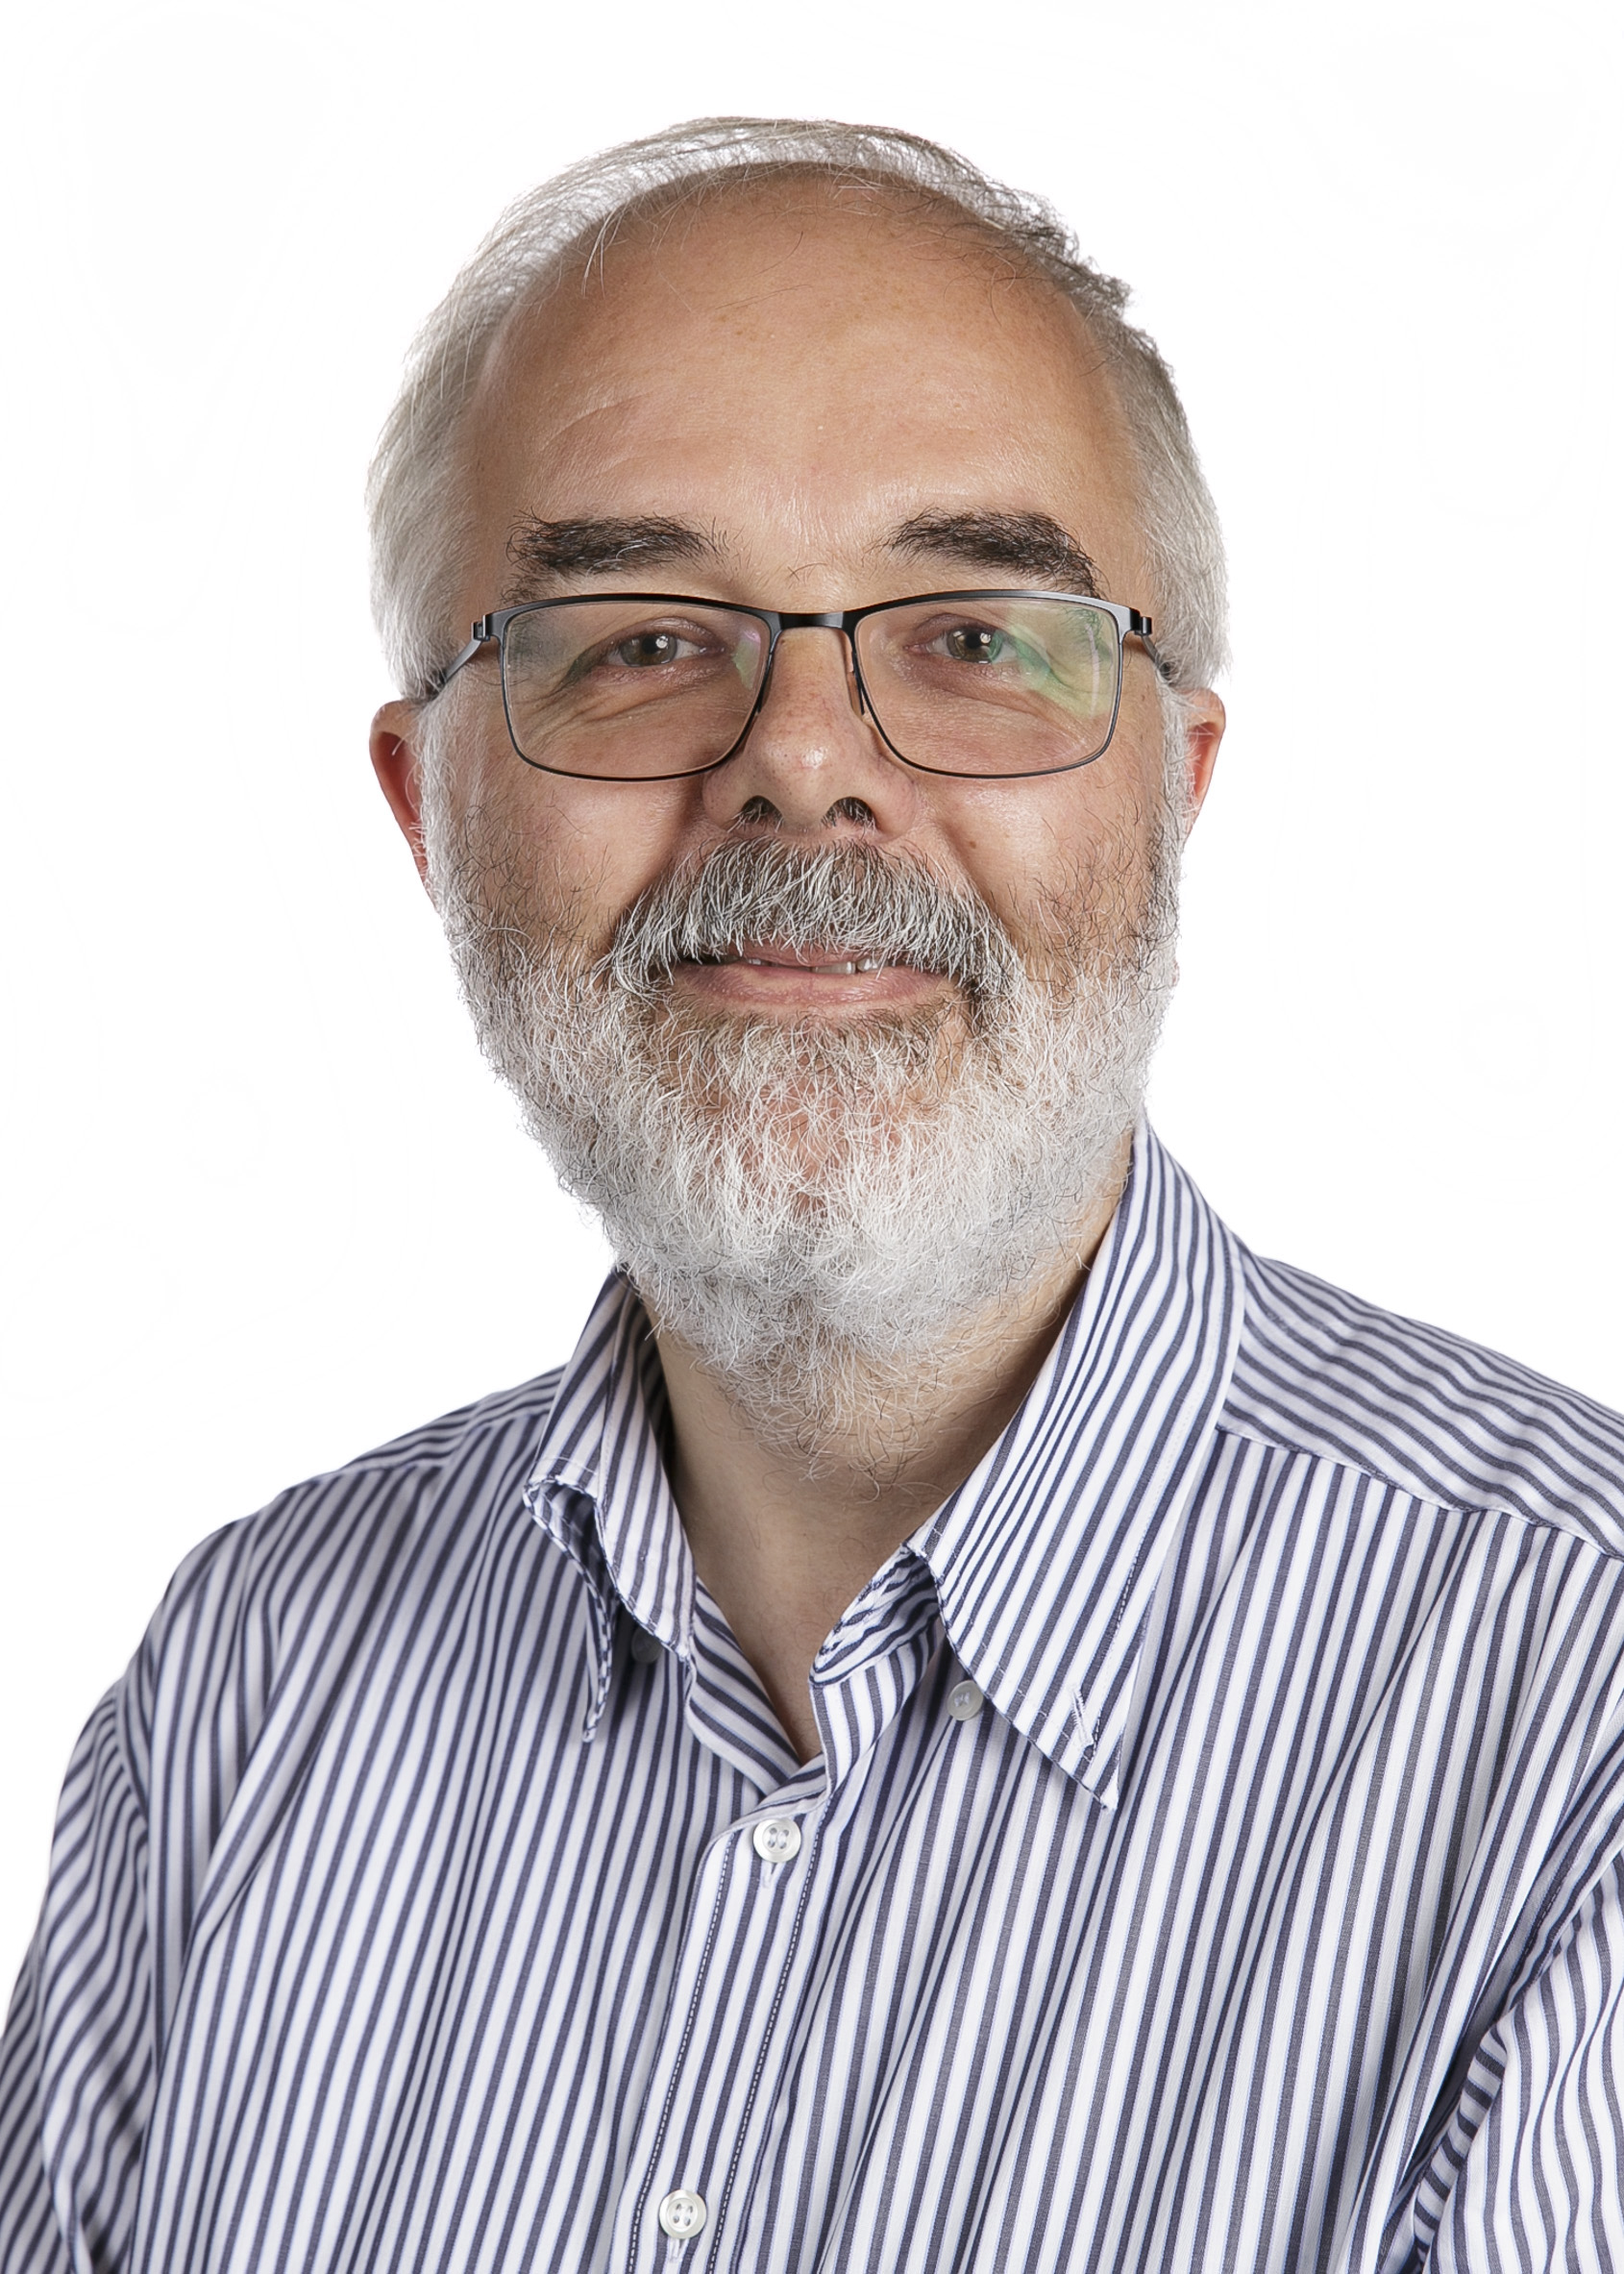
\includegraphics[width=.85\textwidth]{../book/images/helmut}
\end{column}
\end{columns}
\end{frame}

\begin{frame}
\frametitle{Insight is one of the largest data research and innovation centres in Europe...}

\includegraphics[width=\textwidth]{../assistantse/onepage}
\end{frame}

\begin{frame}
\frametitle{European Digital Innovation Hubs Network}
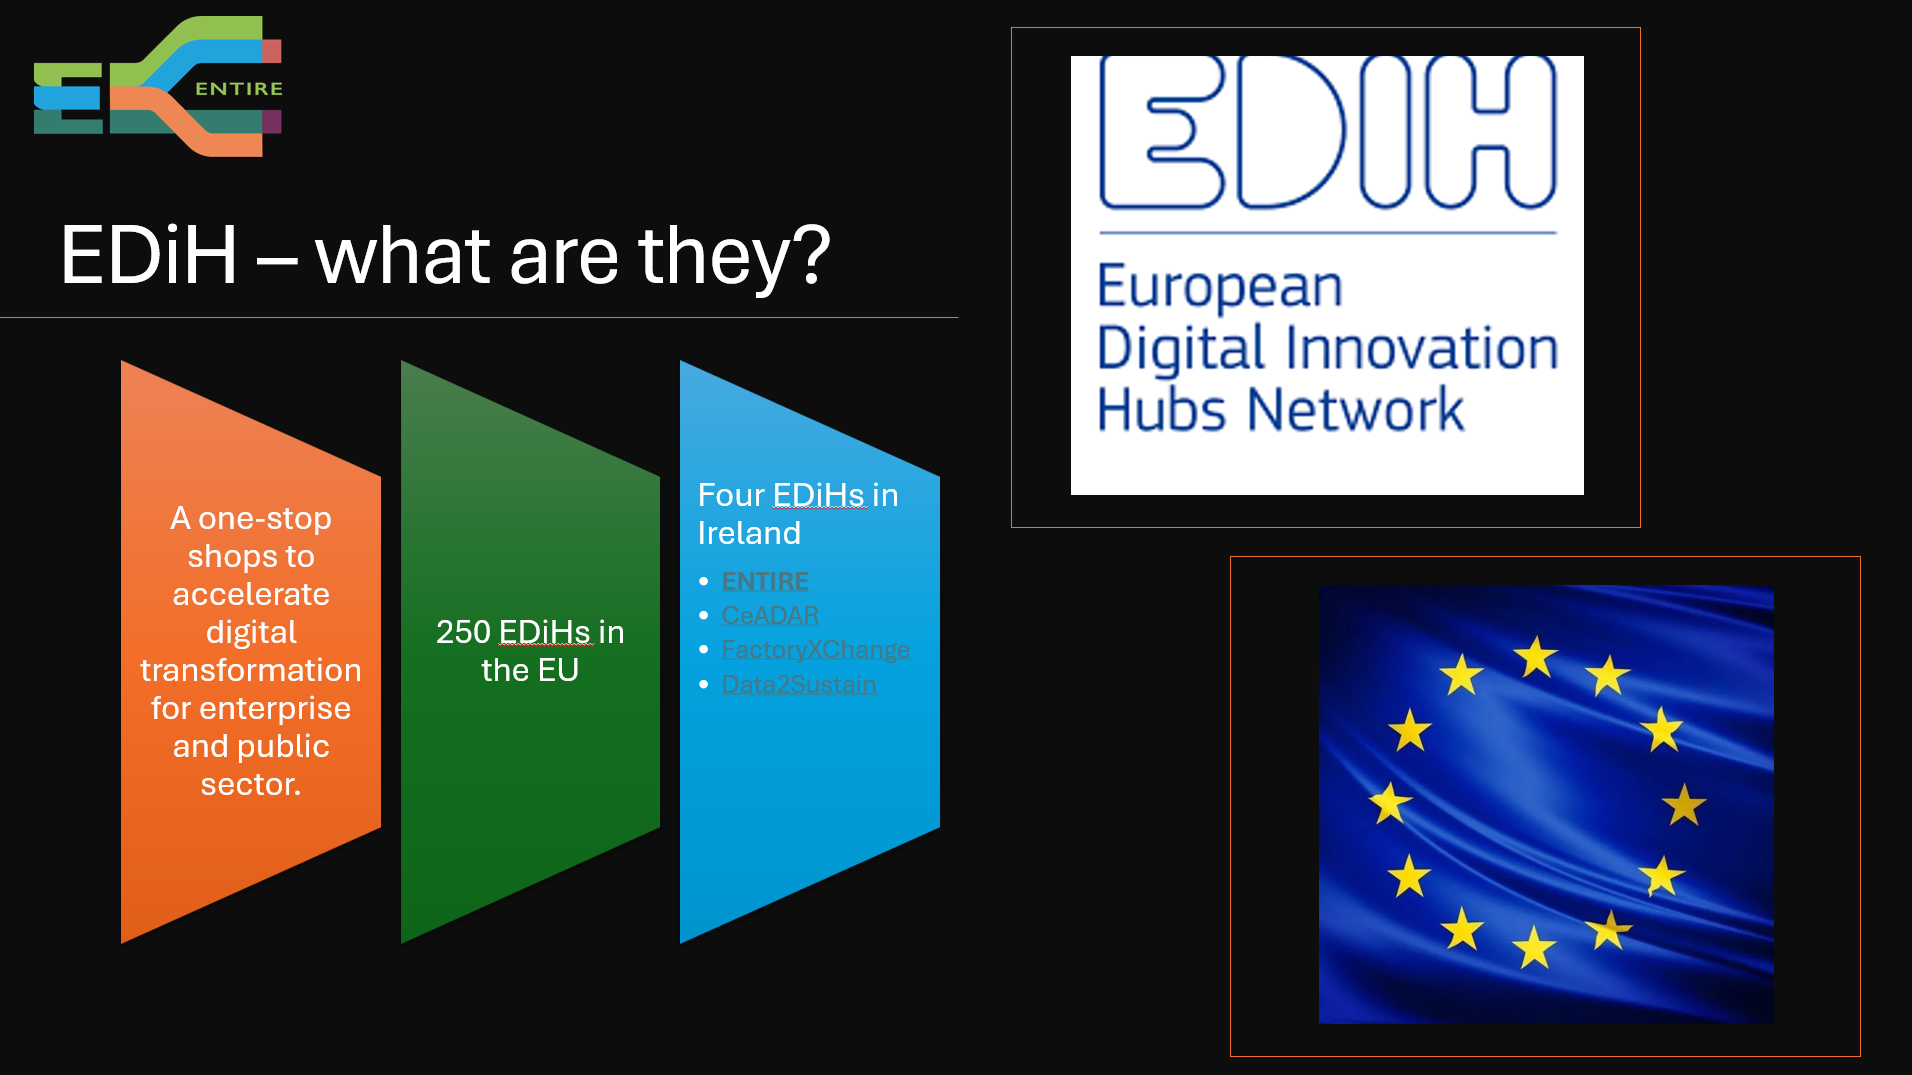
\includegraphics[width=\textwidth]{images/entireoverview}
\url{https://entire-edih.ie/}
\end{frame}

\begin{frame}
\frametitle{ENTIRE at UCC}
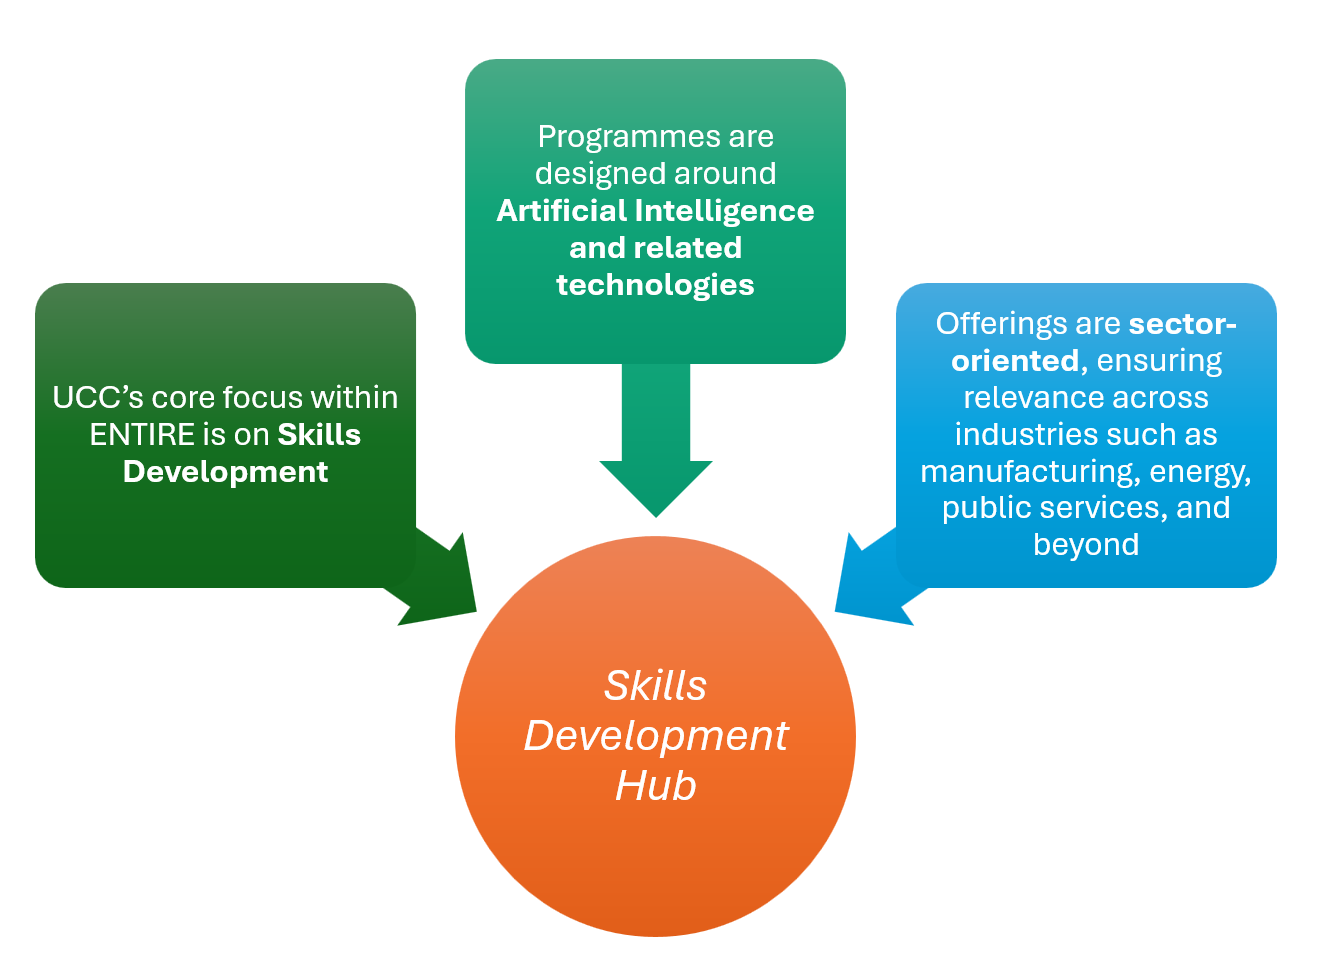
\includegraphics[width=.8\textwidth]{images/skillsdevelopmenthub}
\end{frame}

\begin{frame}
\frametitle{Constraint Programming - in a nutshell}
\begin{itemize}
\item Declarative description of problems with
\begin{itemize}
\item {\em Variables} which range over (finite) sets of values
\item {\em Constraints} over subsets of variables which restrict possible value combinations
\item A {\em solution} is a value assignment which satisfies all constraints
\end{itemize}

\item Constraint propagation/reasoning
\begin{itemize}
\item Removing inconsistent values for variables
\item Detect failure if constraint can not be satisfied
\item Interaction of constraints via shared variables
\item Incomplete
\end{itemize}

\item Search
\begin{itemize}
\item User controlled assignment of values to variables
\item Each step triggers constraint propagation 
\end{itemize}
\item Different domains require/allow different methods
\end{itemize}
\end{frame}

\begin{frame}
  \frametitle{Constraint Programming is Different}
  \begin{itemize}
  \item Declarative Programming
    \begin{itemize}
    \item Concentrate on what you want
      \item Not how to get there
      \item Program != Algorithm
      \item Program = Model
    \end{itemize}
    \item Applied to Combinatorial Problems
      \begin{itemize}
        \item No complete polynomial algorithms known (exist?)
        \item CP less ad-hoc than heuristics
        \item Models can evolve
  \end{itemize}
  \end{itemize}
  \end{frame}
    
\begin{frame}
  \frametitle{A Subtractive Process}
  \begin{textblock}{4}(8,-3)
    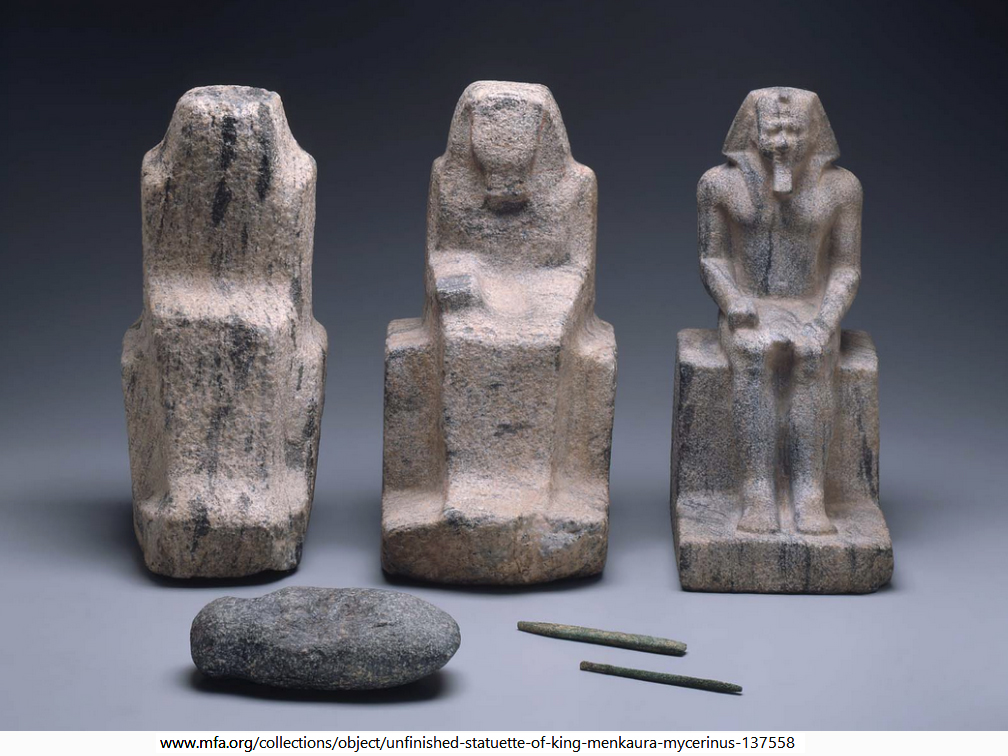
\includegraphics[width=4cm]{../01-introduction/images/stages}
  \end{textblock}
  \vfill
  \begin{quote}
    ``Oh, bosh, as Mr. Ruskin says. Sculpture, per se, is the simplest thing in the world. All you have to do is to take a big chunk of marble and a hammer and chisel, make up your mind what you are about to create and chip off all the marble you don't want.''-Paris Gaulois.
  \end{quote}
  
  {\tiny Source: \url{https://quoteinvestigator.com/2014/06/22/chip-away/}}
\end{frame}




\section{Siemens Energy Case Study (ASSISTANT)}

\begin{frame}
\frametitle{ASSISTANT Project Overview}
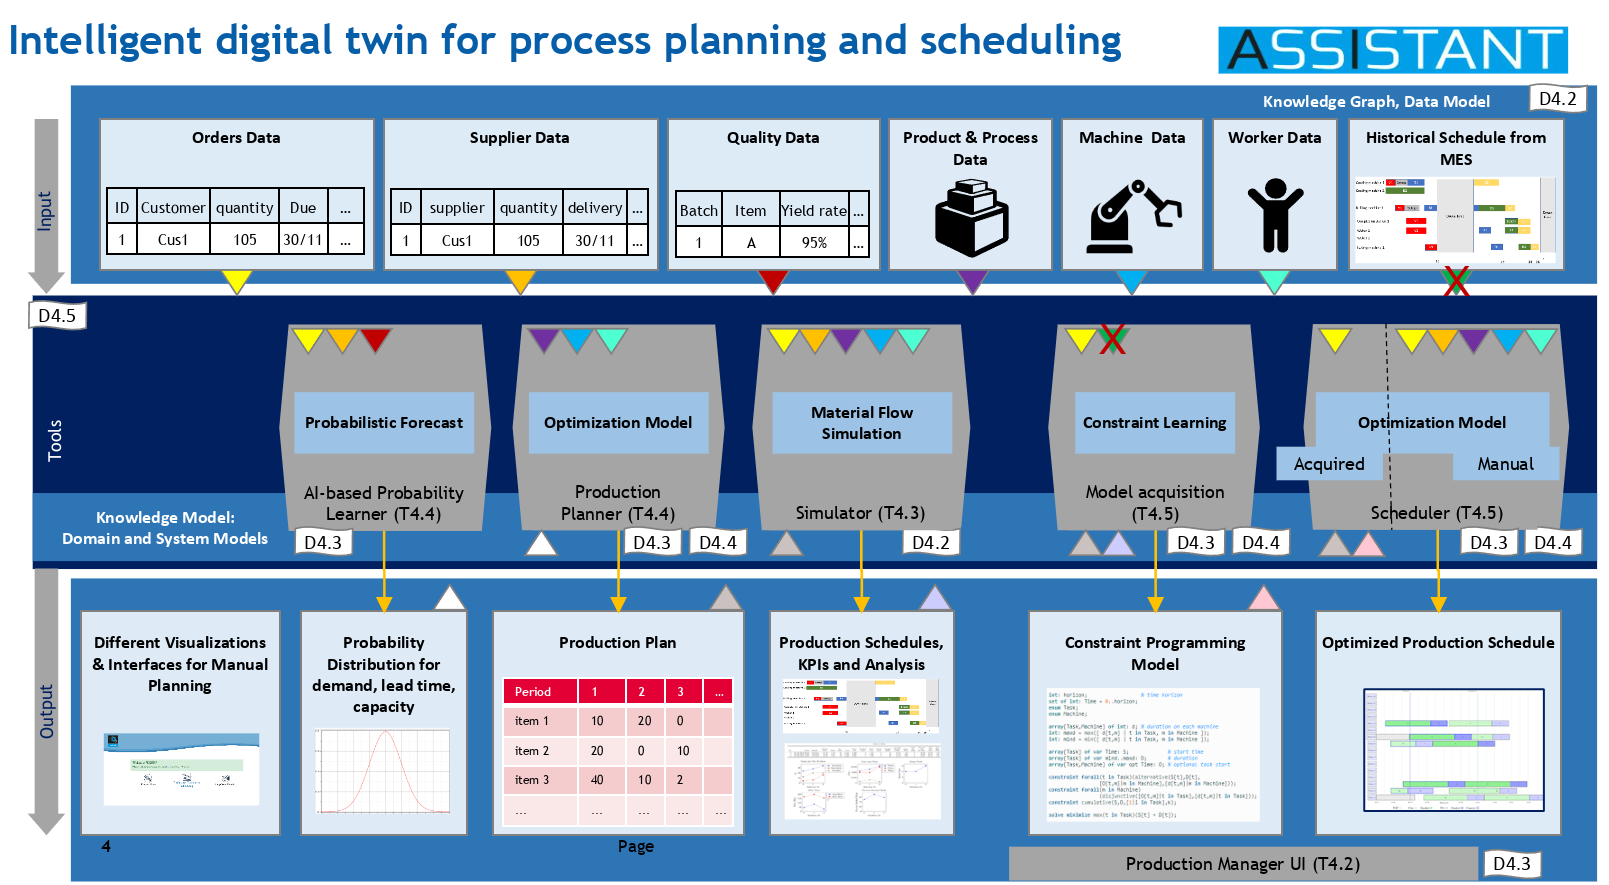
\includegraphics[width=.9\textwidth]{../assistantse/imagesse/assistantdigitaltwin}
\end{frame}

\begin{frame}
\frametitle{Assistant Siemens Energy Use Case}
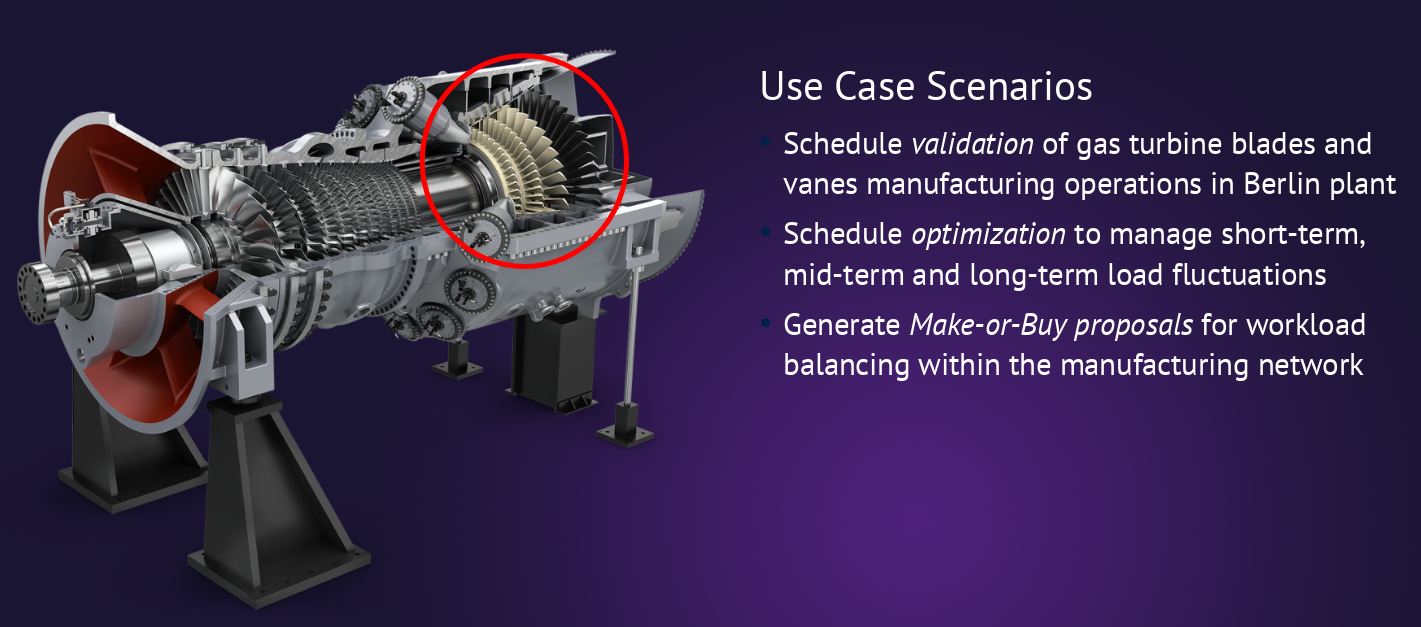
\includegraphics[width=\textwidth]{../assistantse/imagesse/assistantgasturbine}
\end{frame}

\begin{frame}
\frametitle{SE Product Routing}
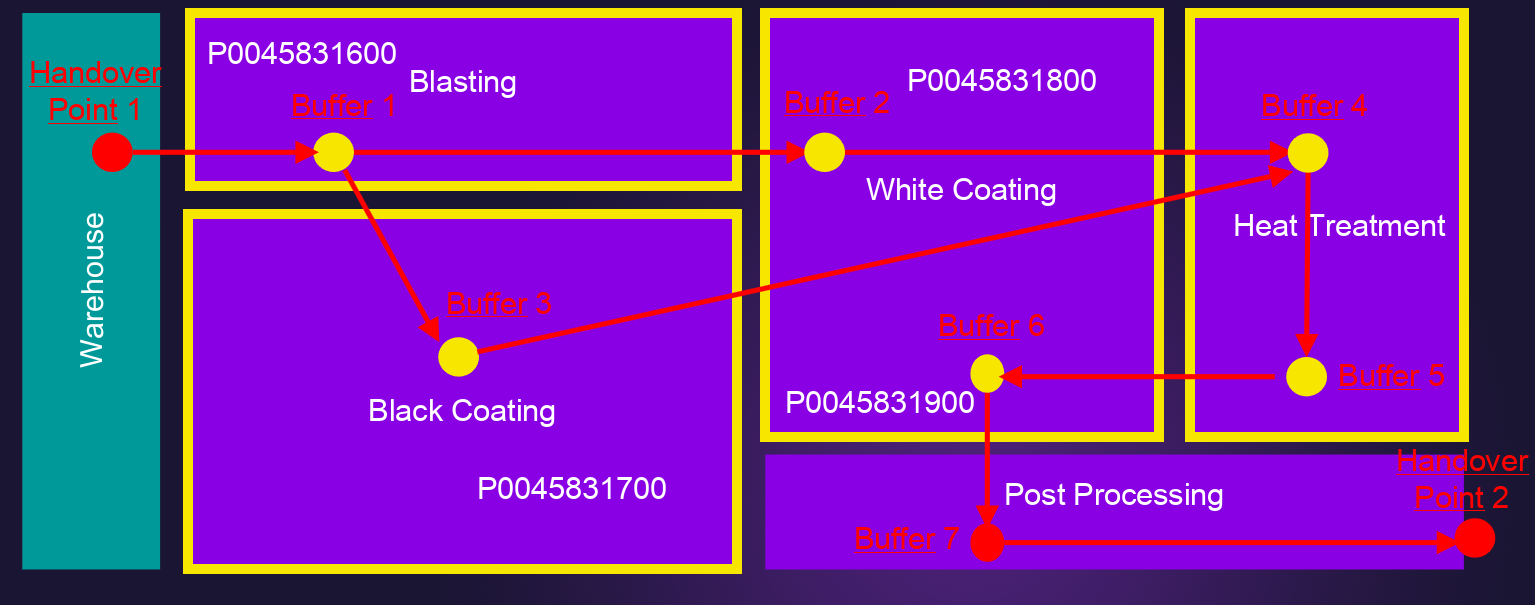
\includegraphics[width=\textwidth]{../assistantse/imagesse/assistantrouting}
\end{frame}

\begin{frame}
\frametitle{Test Datasets}
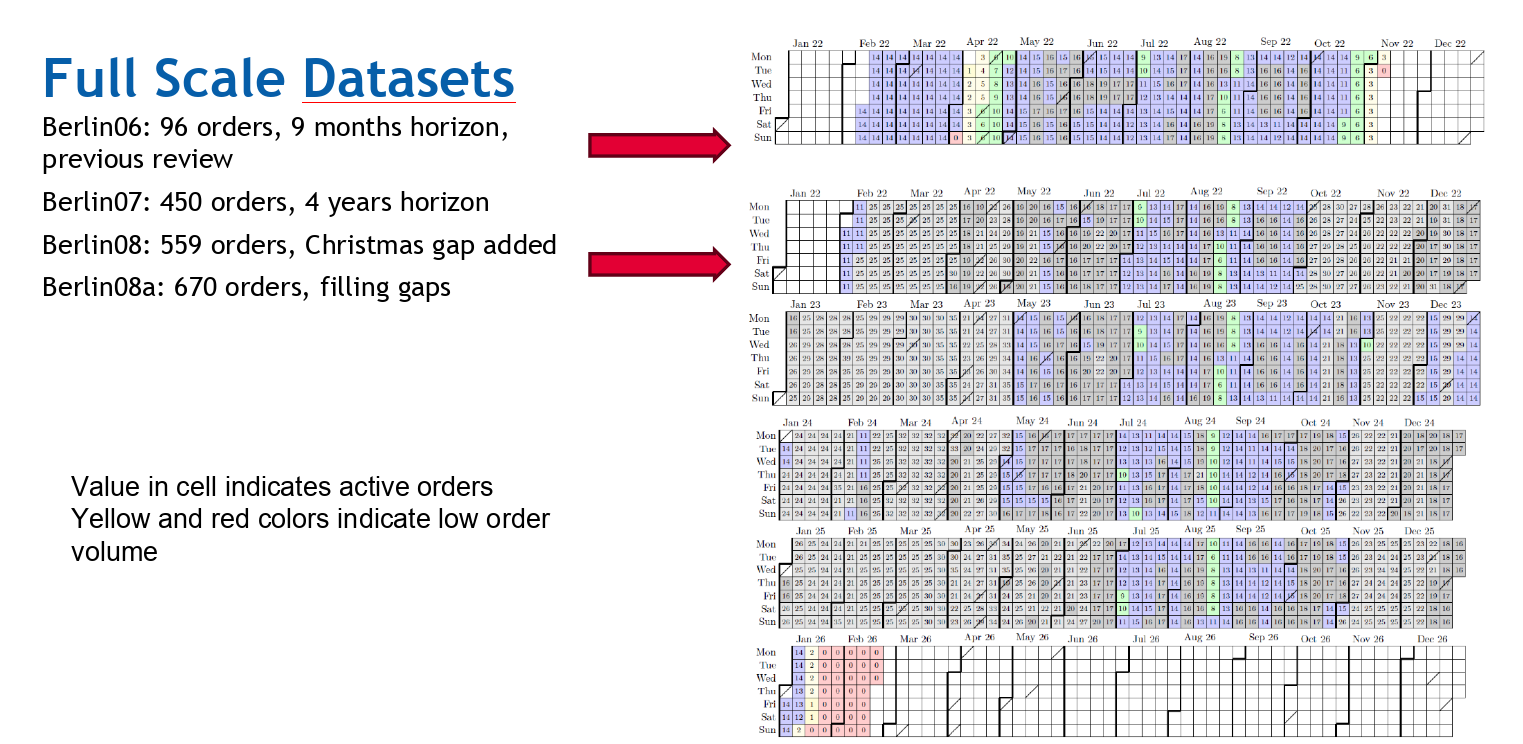
\includegraphics[width=\textwidth]{../assistantse/imagesse/assistantfullscaledatasets}
\end{frame}

\begin{frame}
\frametitle{Optimizer High Level Structure}

\includegraphics[width=.9\textwidth]{../assistantse/imagesse/overview}
\end{frame}

\begin{frame}
\frametitle{Raw Data - Manual Data Entry Causes Problems}
\begin{columns}
\begin{column}{0.65\textwidth}
\begin{itemize}
\item Raw data come from spreadsheet
\begin{itemize}
\item 20 tabs
\end{itemize}
\item Excel is a particularly bad input data format
\item Realistic, not real data
\item Created by hand/automatically from existing test scenarios
\item Series of files Berlin01 - Berlin05 were too inconsistent to run
\item Berlin06 still contains some errors
\item Optimizer explains all issues that it finds
\end{itemize}
\end{column}
\begin{column}{0.35\textwidth}
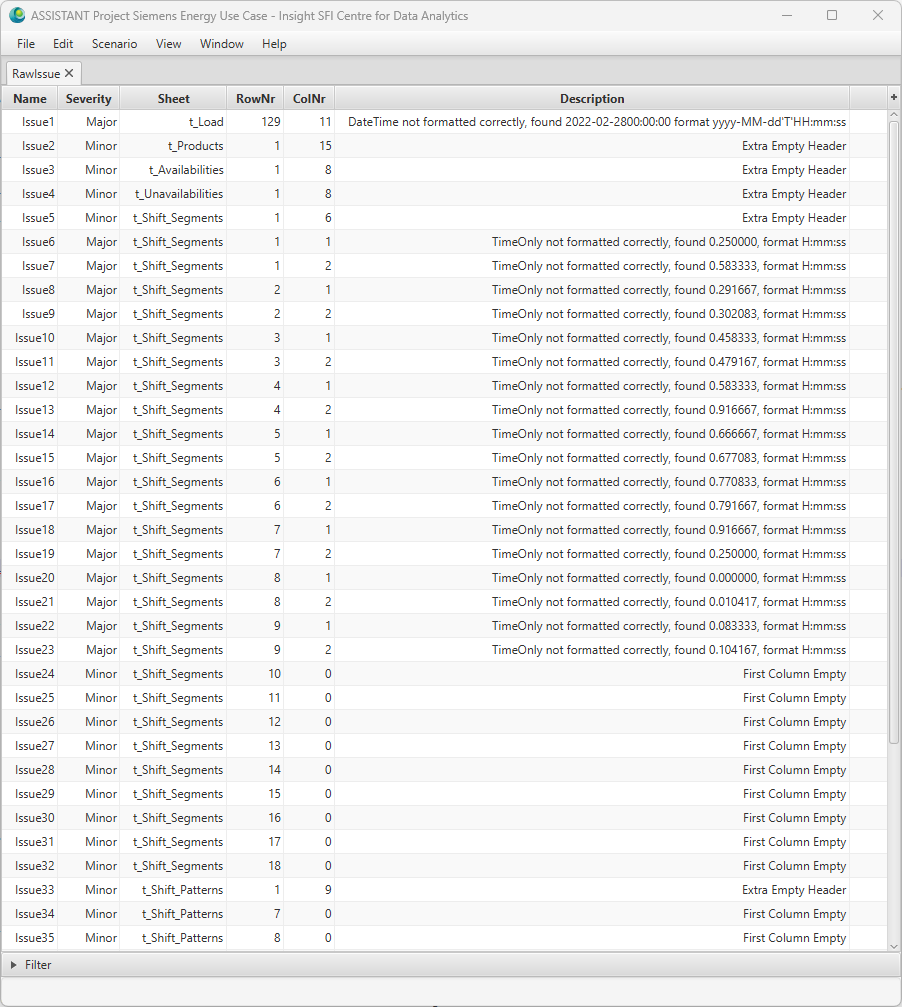
\includegraphics[width=\textwidth]{../assistantse/imagesse/rawerror}
\end{column}
\end{columns}
\end{frame}

\begin{frame}
\frametitle{Domain Model - Knowledge Graph}
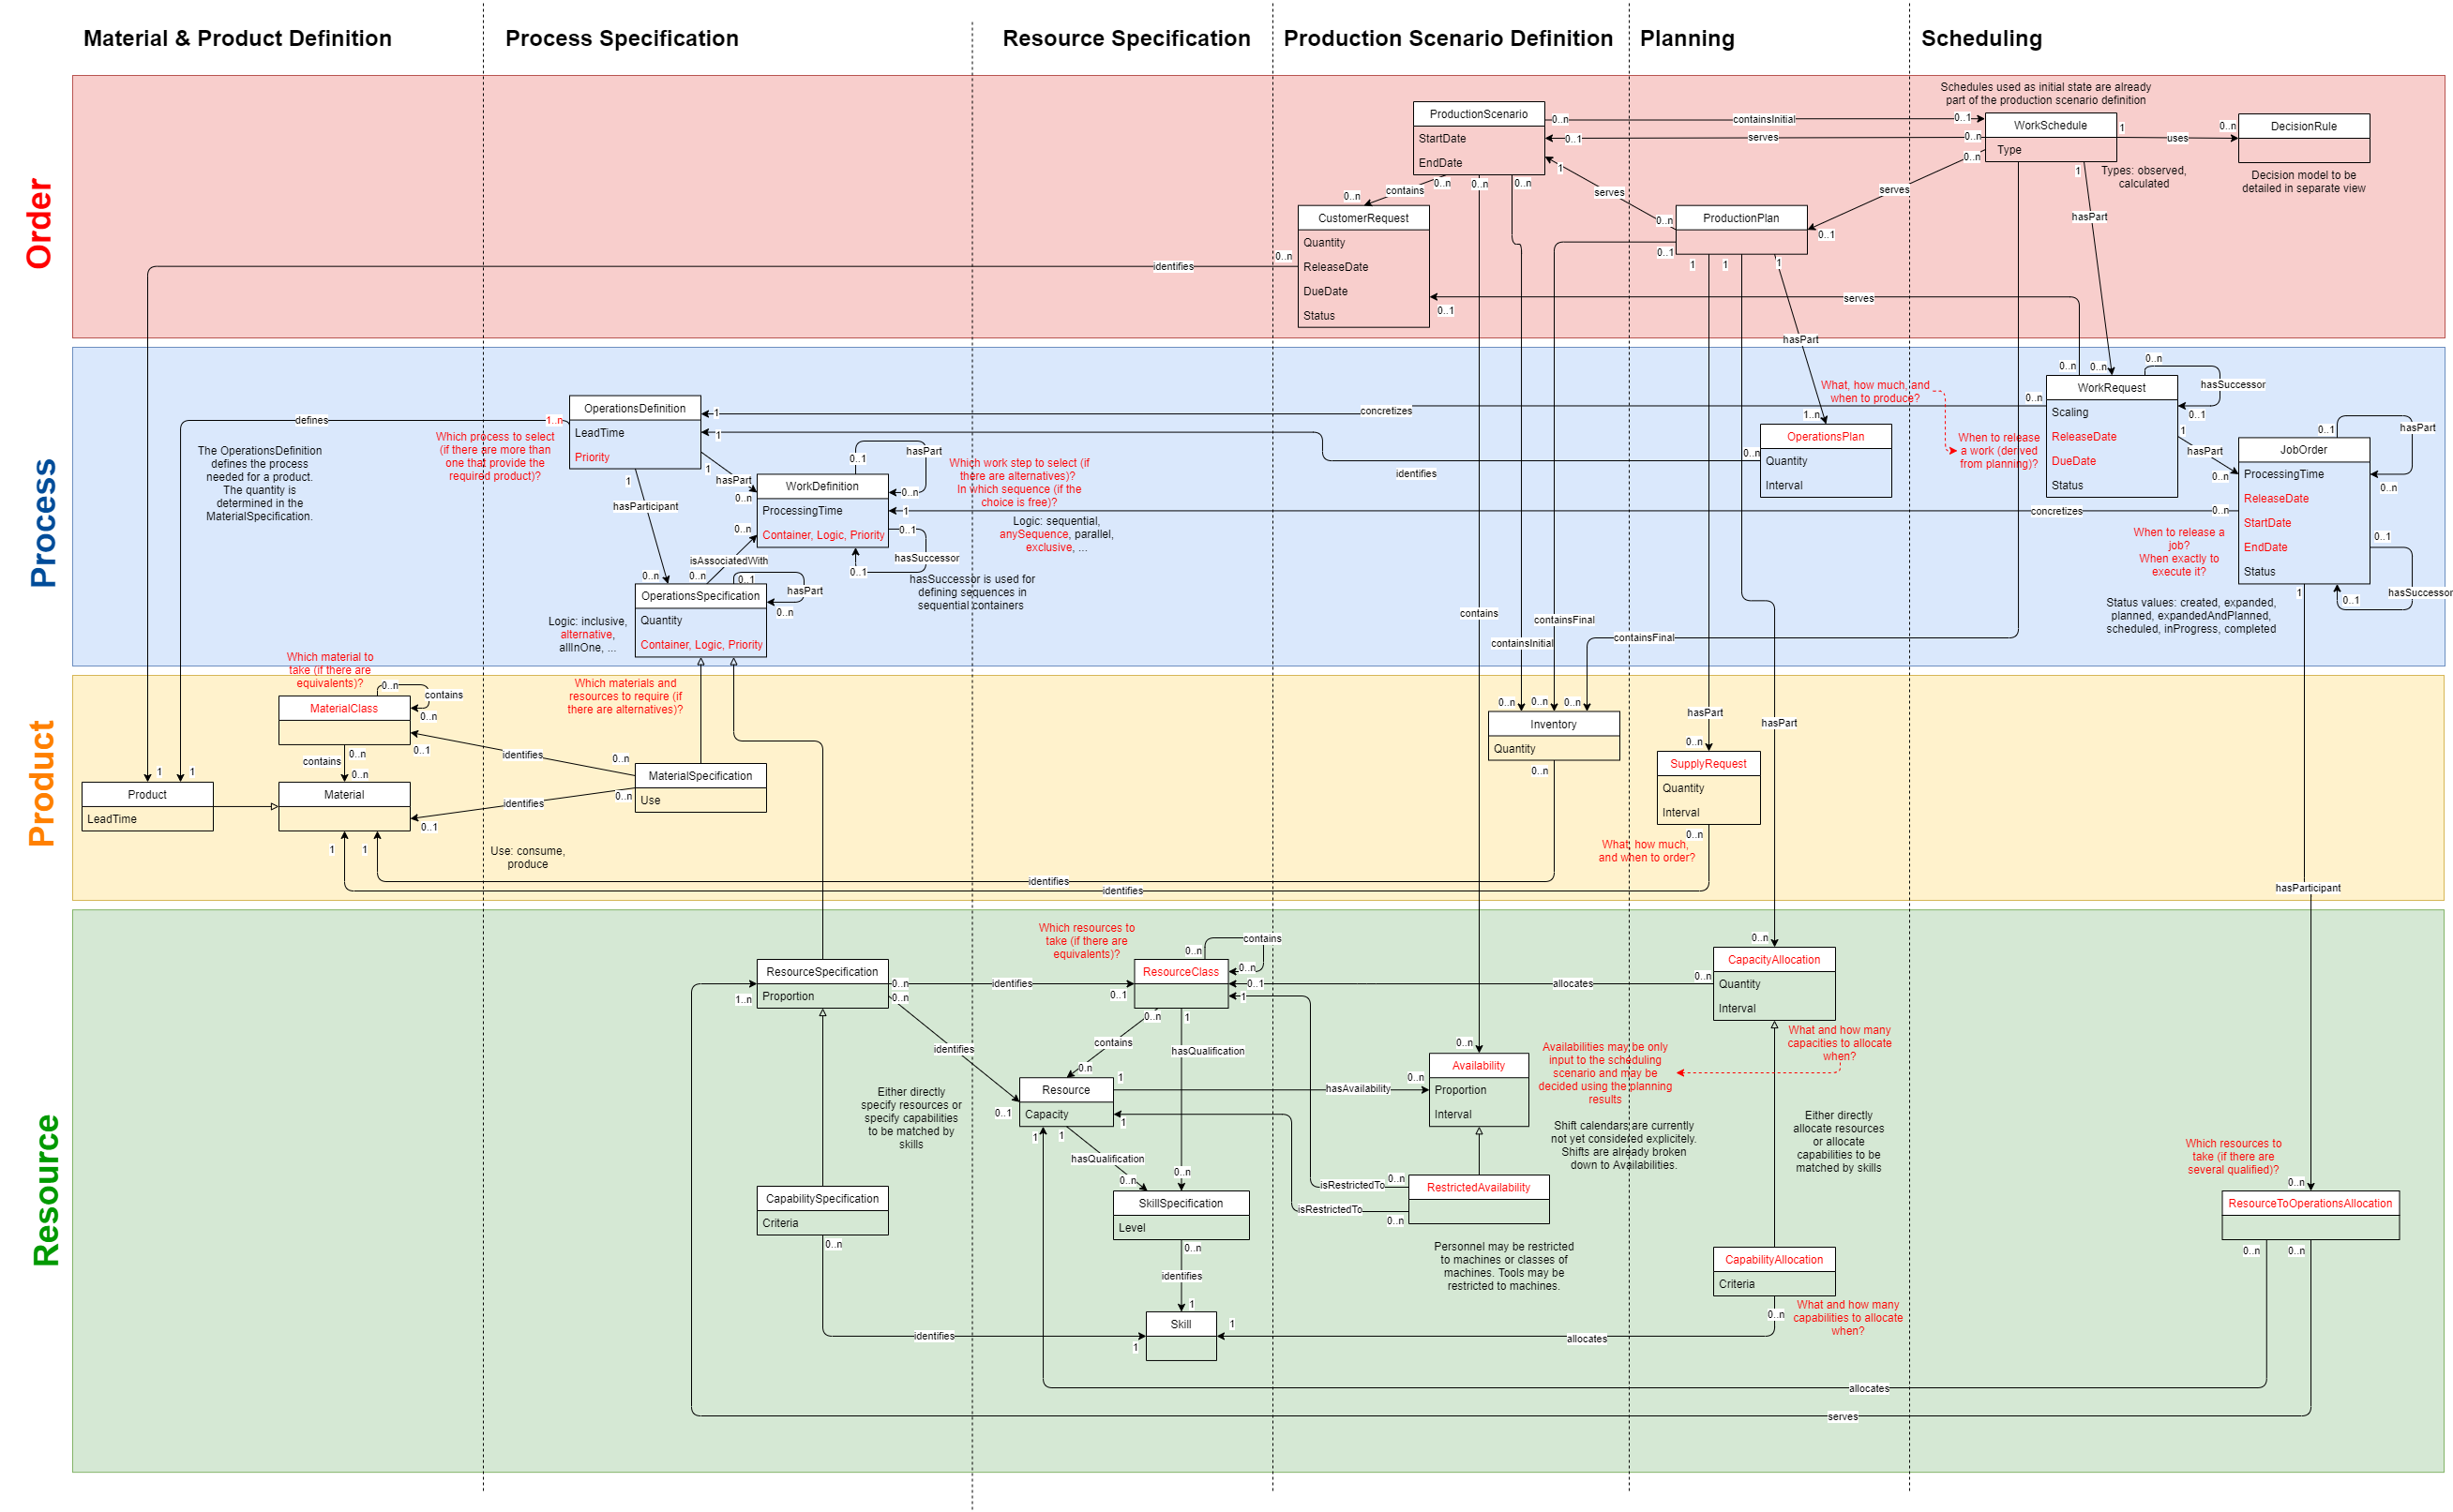
\includegraphics[width=\textwidth]{../assistantse/imagesse/DomainModel}

Developed with Siemens, Siemens Energy
\end{frame}

\begin{frame}
\frametitle{Solution for Berlin 08a - Shows Only\\20\% of Tasks in Model}
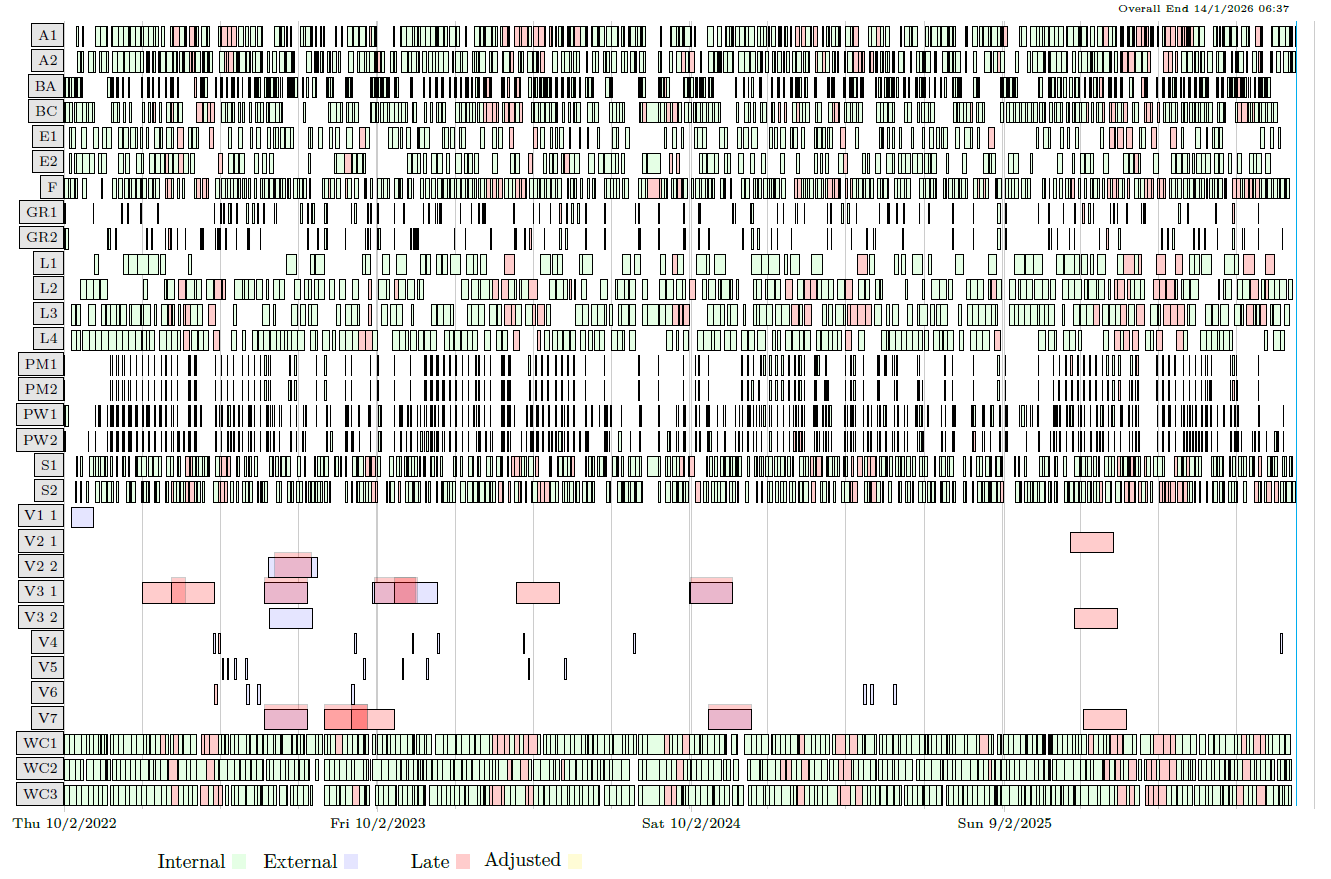
\includegraphics[width=.95\textwidth]{../assistantse/imagesse/solution08apref2}
\end{frame}

\begin{frame}
\frametitle{Implementation}
\begin{itemize}
\item Requirement capture done inside project
\item Data checking/cleaning most time consuming aspect
\item Some specified functionality was rejected by Betriebsrat
\item Built in Java
\item Uses IBM's CPOptimizer back-end
\begin{itemize}
\item Logical choice based on required features
\item Choice created issues later in project
\end{itemize}
\item 120k LoC, 110k generated, 3k solver
\item Outperforms both 
\begin{itemize}
\item Current in-house tool
\item Simulation based tool based on commercial simulator 
\end{itemize}
\item System installed at SE site, but not in daily use
\end{itemize}
\end{frame}

\begin{frame}
\frametitle{Advanced Feature: Explaining Late Delivery}
\begin{itemize}
\item Explain why some orders are delivered late
\item Find root-cause, show schedule in context
\end{itemize}

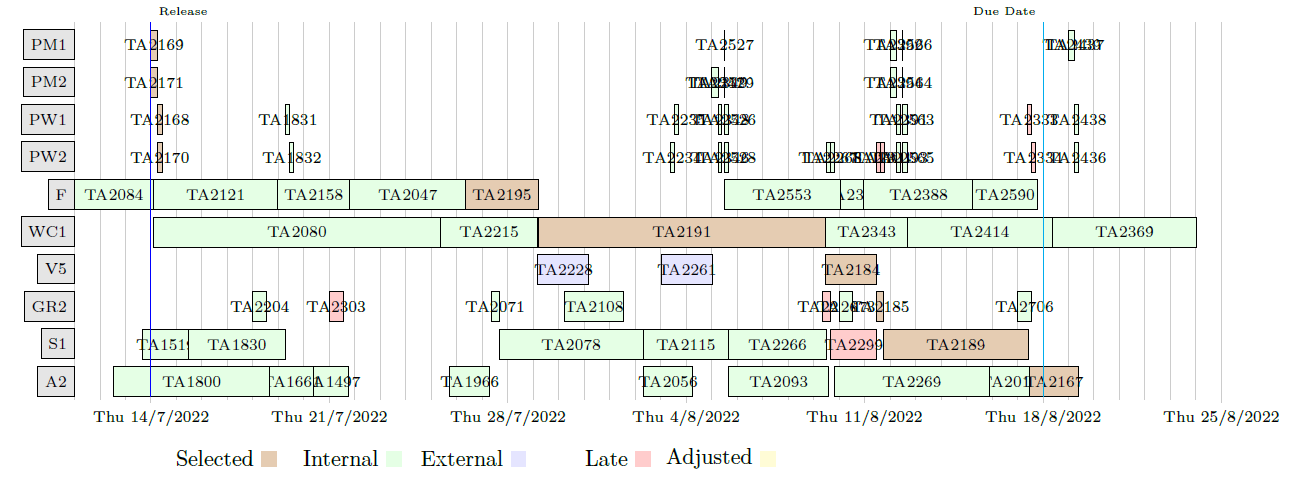
\includegraphics[width=\textwidth]{../assistantse/imagesse/explanation}
\end{frame}

\begin{frame}
\frametitle{Evaluation - KPIs}
\begin{tabular}{p{6cm}rrr}\toprule
KPI & Baseline & Optimizer \\ \midrule
OTD (On-time delivery)& > 80 \%  & 92 \%\\
Bottleneck machine utilization & 99.5 \% & 100 \%\\
Manufacturing defects & 10-15 \% & < 10 \%\\
Scenarios in 8 hours & 15-20 & > 100,000 \\
\bottomrule
\end{tabular}
\end{frame}


\begin{frame}
\frametitle{CPO Keeps on Trucking}
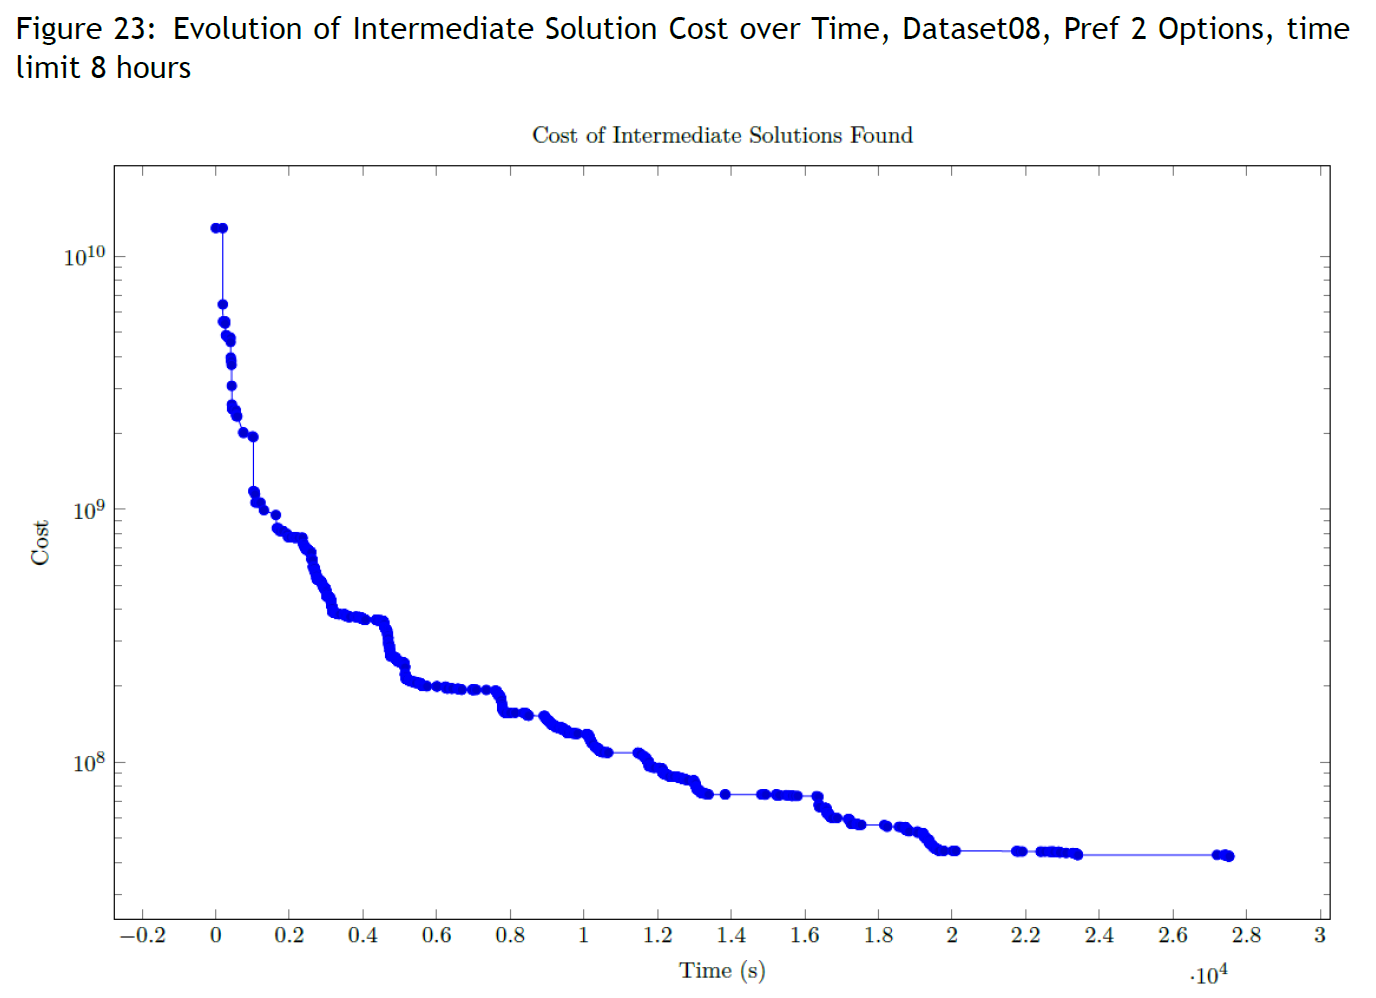
\includegraphics[width=.9\textwidth]{../assistantse/imagesse/improving}
\end{frame}

\begin{frame}
\frametitle{Conclusion by Siemens Energy}

\includegraphics[width=\textwidth]{../assistantse/imagesse/quote}

{\tiny from ASSISTANT final project review: Siemens Energy assessment}
\end{frame}

\section{IHTC 2024}

\begin{frame}
\frametitle{Hospital Capacity Management}
\begin{itemize}
\item Decide which patients to admit in planning period (2-4 weeks)
\item Decide when to admit selected patients
\item Surgery performed on day of admission by preassigned surgeon
\item Respect capacity constraints of surgeons and theatres
\item Assign bed to patient during their stay
\item Respect constraints on room capacity and use
\item Assign nurses to rooms in each shift to provide required care
%\item Nurse roster given
\item Minimise total, weighted cost
\end{itemize}
\end{frame}

\subsection{IHTC 2024 Competition}

\begin{frame}
\frametitle{IHTC 2024}
\begin{itemize}
\item \url{https://ihtc2024.github.io/}
\item Organized by Udine/Italy and KU Leuven/Belgium
\item Under EURO umbrella (replaced Roadef 2024)
\item Ran from September 2024 to March 2025
\item 32 teams participating
\item 70 problem instances
\end{itemize}
\end{frame}

\begin{frame}
\frametitle{IHTC2024 Winners}
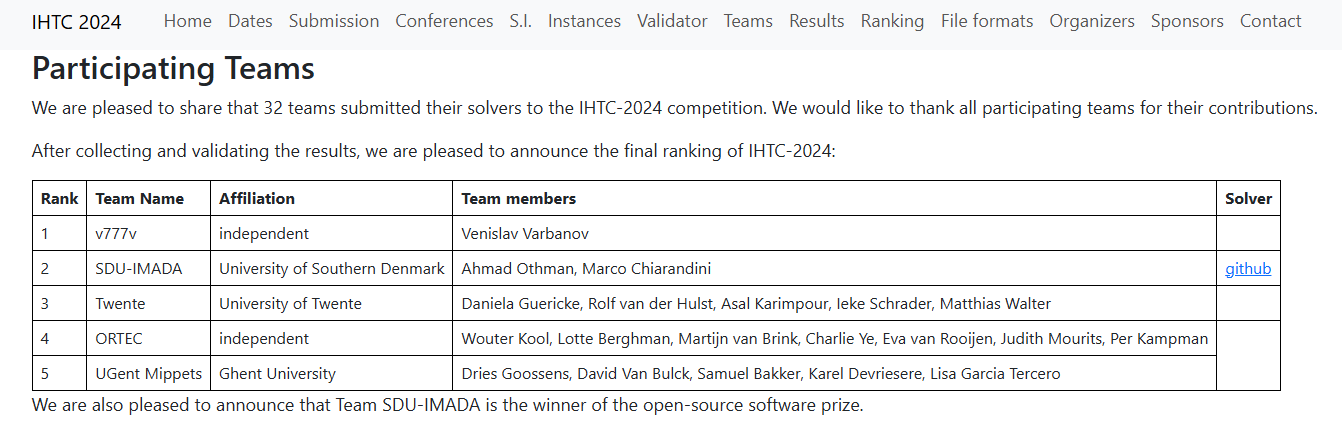
\includegraphics[width=\textwidth]{../schedulingseminar/ihtc2024/ihtc2024winners}
\end{frame}

\begin{frame}
\frametitle{Is this a good problem for CP?}
\begin{itemize}
\item There are good and bad points
\item Good
\begin{itemize}
\item Not too messy
\item Problem size not super large
\item Decomposes into well-known sub problem types
\end{itemize}
\item Bad
\begin{itemize}
\item Some constraints are totally soft
\item Overall cost is weighted sum of many factors
\item Time resolution limited
\end{itemize}
\end{itemize}
\end{frame}


\subsection{Concepts}

\begin{frame}
\frametitle{Concepts}
\begin{itemize}
\item Time
\item Patients/Occupants
\item Surgeons
\item Nurses
\item Operating theatres
\item Rooms/beds
\end{itemize}
\end{frame}

% \begin{frame}
% \frametitle{Data Samples}
% \begin{itemize}
% \item We will use two problem instances to show features of problems
% \item test10, largest of the initial instance set
% \item m29, largest of the final evaluation set
% \item Demonstrate scalability of visualisation as well as of solvers
% \end{itemize}
% \end{frame}

% \begin{frame}[fragile]
% \frametitle{Time Scale (Planning period 2-4 weeks)}
% 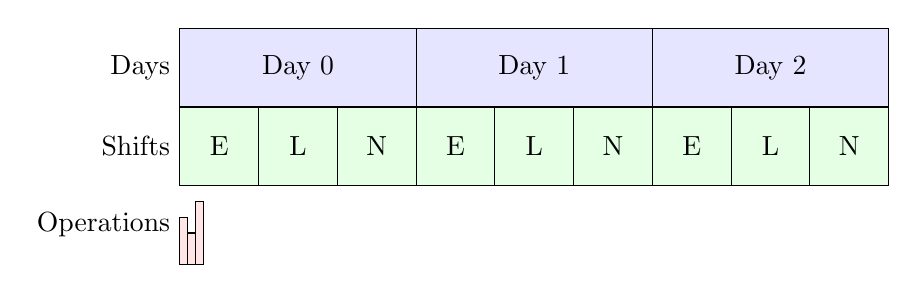
\begin{tikzpicture}
\node[left] at (0,2.5) {Days};
\node[left] at (0,1.5) {Shifts};
\node[left] at (0,0.5) {Operations};
\draw[fill=blue!10,draw=black] (0,2) rectangle node {Day 0} (3,3);
\draw[fill=blue!10,draw=black] (3,2) rectangle node {Day 1} (6,3);
\draw[fill=blue!10,draw=black] (6,2) rectangle node {Day 2} (9,3);
\draw[fill=green!10,draw=black] (0,1) rectangle node {E} (1,2);
\draw[fill=green!10,draw=black] (1,1) rectangle node {L} (2,2);
\draw[fill=green!10,draw=black] (2,1) rectangle node {N} (3,2);
\draw[fill=green!10,draw=black] (3,1) rectangle node {E} (4,2);
\draw[fill=green!10,draw=black] (4,1) rectangle node {L} (5,2);
\draw[fill=green!10,draw=black] (5,1) rectangle node {N} (6,2);
\draw[fill=green!10,draw=black] (6,1) rectangle node {E} (7,2);
\draw[fill=green!10,draw=black] (7,1) rectangle node {L} (8,2);
\draw[fill=green!10,draw=black] (8,1) rectangle node {N} (9,2);
\draw[fill=red!10,draw=black] (0,0) rectangle  (0.1,0.6);
\draw[fill=red!10,draw=black] (0.1,0) rectangle  (0.2,0.4);
\draw[fill=red!10,draw=black] (0.2,0) rectangle  (0.3,0.8);
\end{tikzpicture}

% \begin{itemize}
% \item Three different time scales in problem
% \begin{itemize}
% \item Days: patient admission, bed/room use, aligned with shifts
% \item Shifts: Nurse assignment, workload, skills
% \item Procedures: not scheduled, only total load per day
% \end{itemize}
% \end{itemize}
% \end{frame}

% \begin{frame}
% \frametitle{Patients}
% \begin{itemize}
% \item Potential inpatients for surgery, assigned to a surgeon
% \item Mandatory patients must be scheduled
% \item Optional patients may be scheduled
% \item Each patient has earliest admission day (release day)
% \item Mandatory patients have a latest admission day (due date)
% \item Procedure length and length of stay vary
% \end{itemize}
% \end{frame}

% \begin{frame}[fragile]
% \frametitle{Patient Events and Intervals}
% \scalebox{0.85}{
% 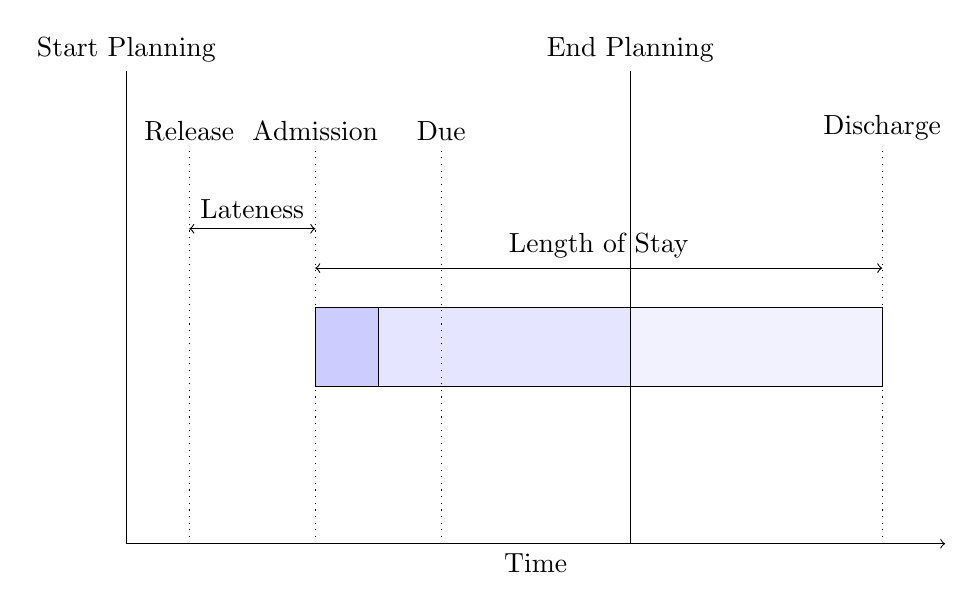
\begin{tikzpicture}[xscale=0.8,yscale=1.0]
\draw[->] (0,0) -- node[below]{Time}(13,0);

\draw[fill=blue!20] (3,2) rectangle (4,3);
\draw[fill=blue!10] (4,2) rectangle (8,3);
\draw[fill=blue!5] (8,2) rectangle (12,3);
\node[above] at (0,6) {Start Planning};
\node[above] at (1,5) {Release};
\node[above] at (3,5) {Admission};
\node[above] at (5,5) {Due};
\node[above] at (8,6) {End Planning};
\node[above] at (12,5) {Discharge};
\draw[] (0,0) -- (0,6);
\draw[dotted] (1,0) -- (1,5);
\draw[dotted] (3,0) -- (3,5);
\draw[dotted] (5,0) -- (5,5);
\draw[] (8,0) -- (8,6);
\draw[dotted] (12,0) -- (12,5);
\draw[<->] (3,3.5) -- node[above] {Length of Stay} (12,3.5);
\draw[<->] (1,4) -- node[above] {Lateness} (3,4);
\end{tikzpicture}

% }
% \end{frame}

\begin{frame}[fragile]
\frametitle{Needed Patient Care on Day of Stay, Top 20 Patients in test10}
\scalebox{0.5}{
{\scriptsize
\begin{tabular}{l*{63}{r}} \toprule
& 0E& 0L& 0N& 1E& 1L& 1N& 2E& 2L& 2N& 3E& 3L& 3N& 4E& 4L& 4N& 5E& 5L& 5N& 6E& 6L& 6N& 7E& 7L& 7N& 8E& 8L& 8N& 9E& 9L& 9N& 10E& 10L& 10N& 11E& 11L& 11N& 12E& 12L& 12N& 13E& 13L& 13N& 14E& 14L& 14N& 15E& 15L& 15N& 16E& 16L& 16N& 17E& 17L& 17N& 18E& 18L& 18N& 19E& 19L& 19N& 20E& 20L& 20N\\ \midrule 
p301& \cellcolor{red!10!}3& \cellcolor{blue!10}3& \cellcolor{black!10}1& \cellcolor{blue!10}2& \cellcolor{white}3& \cellcolor{yellow!10}1& \cellcolor{black!10}2& \cellcolor{black!10}2& \cellcolor{blue!10}1& \cellcolor{yellow!10}2& \cellcolor{black!10}3& \cellcolor{white}2& \cellcolor{red!10!}3& \cellcolor{white}2& \cellcolor{blue!10}2& \cellcolor{white}2& \cellcolor{red!10!}3& \cellcolor{white}1& \cellcolor{black!10}2& \cellcolor{black!10}2& \cellcolor{white}2& \cellcolor{blue!10}3& \cellcolor{yellow!10}3& \cellcolor{black!10}1& \cellcolor{white}3& \cellcolor{red!10!}2& \cellcolor{white}1& \cellcolor{blue!10}3& \cellcolor{black!10}2& \cellcolor{black!10}1& \cellcolor{yellow!10}2& \cellcolor{white}2& \cellcolor{yellow!10}2& \cellcolor{black!10}2& \cellcolor{blue!10}1& \cellcolor{white}2& \cellcolor{red!10!}2& \cellcolor{white}1& \cellcolor{blue!10}2& & & & & & & & & & & & & & & & & & & & & & & & \\ 
p121& \cellcolor{red!10!}2& \cellcolor{blue!10}2& \cellcolor{black!10}2& \cellcolor{black!10}2& \cellcolor{yellow!10}3& \cellcolor{yellow!10}2& \cellcolor{red!10!}2& \cellcolor{black!10}3& \cellcolor{white}1& \cellcolor{white}2& \cellcolor{black!10}3& \cellcolor{white}2& \cellcolor{red!10!}3& \cellcolor{black!10}3& \cellcolor{white}2& \cellcolor{white}3& \cellcolor{black!10}2& \cellcolor{white}1& \cellcolor{white}2& \cellcolor{blue!10}2& \cellcolor{blue!10}2& \cellcolor{white}3& \cellcolor{white}2& \cellcolor{white}1& \cellcolor{blue!10}3& \cellcolor{red!10!}2& \cellcolor{white}1& \cellcolor{yellow!10}2& \cellcolor{blue!10}2& \cellcolor{black!10}2& \cellcolor{blue!10}3& \cellcolor{blue!10}3& \cellcolor{white}1& \cellcolor{blue!10}3& \cellcolor{yellow!10}2& \cellcolor{black!10}2& & & & & & & & & & & & & & & & & & & & & & & & & & & \\ 
p227& \cellcolor{blue!10}2& \cellcolor{red!10!}2& \cellcolor{white}1& \cellcolor{blue!10}2& \cellcolor{blue!10}2& \cellcolor{yellow!10}1& \cellcolor{blue!10}3& \cellcolor{yellow!10}2& \cellcolor{yellow!10}1& \cellcolor{white}2& \cellcolor{red!10!}3& \cellcolor{white}1& \cellcolor{blue!10}3& \cellcolor{yellow!10}2& \cellcolor{blue!10}2& \cellcolor{black!10}3& \cellcolor{white}3& \cellcolor{white}2& \cellcolor{white}2& \cellcolor{blue!10}3& \cellcolor{white}1& \cellcolor{white}3& \cellcolor{yellow!10}2& \cellcolor{black!10}1& \cellcolor{red!10!}2& \cellcolor{white}3& \cellcolor{yellow!10}1& \cellcolor{white}3& \cellcolor{yellow!10}2& \cellcolor{white}1& \cellcolor{black!10}2& \cellcolor{yellow!10}2& \cellcolor{yellow!10}2& \cellcolor{yellow!10}3& \cellcolor{blue!10}1& \cellcolor{white}2& & & & & & & & & & & & & & & & & & & & & & & & & & & \\ 
p421& \cellcolor{black!10}2& \cellcolor{red!10!}2& \cellcolor{white}1& \cellcolor{red!10!}3& \cellcolor{blue!10}3& \cellcolor{white}2& \cellcolor{black!10}2& \cellcolor{blue!10}2& \cellcolor{white}2& \cellcolor{blue!10}2& \cellcolor{blue!10}2& \cellcolor{yellow!10}1& \cellcolor{yellow!10}2& \cellcolor{black!10}2& \cellcolor{blue!10}1& \cellcolor{red!10!}2& \cellcolor{blue!10}2& \cellcolor{yellow!10}1& \cellcolor{black!10}3& \cellcolor{black!10}2& \cellcolor{blue!10}2& \cellcolor{white}3& \cellcolor{yellow!10}2& \cellcolor{yellow!10}2& \cellcolor{yellow!10}3& \cellcolor{yellow!10}3& \cellcolor{yellow!10}1& \cellcolor{white}3& \cellcolor{blue!10}2& \cellcolor{blue!10}1& \cellcolor{white}2& \cellcolor{yellow!10}2& \cellcolor{yellow!10}1& \cellcolor{blue!10}2& \cellcolor{white}2& \cellcolor{white}1& & & & & & & & & & & & & & & & & & & & & & & & & & & \\ 
p042& \cellcolor{blue!10}2& \cellcolor{red!10!}2& \cellcolor{white}2& \cellcolor{blue!10}2& \cellcolor{black!10}2& \cellcolor{black!10}1& \cellcolor{black!10}2& \cellcolor{white}2& \cellcolor{black!10}2& \cellcolor{red!10!}2& \cellcolor{blue!10}3& \cellcolor{blue!10}1& \cellcolor{white}3& \cellcolor{black!10}2& \cellcolor{blue!10}2& \cellcolor{red!10!}3& \cellcolor{black!10}3& \cellcolor{yellow!10}1& \cellcolor{white}2& \cellcolor{yellow!10}2& \cellcolor{yellow!10}2& \cellcolor{white}2& \cellcolor{yellow!10}3& \cellcolor{yellow!10}1& \cellcolor{blue!10}3& \cellcolor{black!10}2& \cellcolor{black!10}2& \cellcolor{yellow!10}3& \cellcolor{blue!10}2& \cellcolor{blue!10}1& \cellcolor{white}1& \cellcolor{white}2& \cellcolor{white}1& & & & & & & & & & & & & & & & & & & & & & & & & & & & & & \\ 
p062& \cellcolor{black!10}2& \cellcolor{red!10!}3& \cellcolor{white}1& \cellcolor{red!10!}2& \cellcolor{black!10}2& \cellcolor{blue!10}1& \cellcolor{black!10}3& \cellcolor{white}2& \cellcolor{black!10}1& \cellcolor{white}2& \cellcolor{blue!10}2& \cellcolor{white}2& \cellcolor{red!10!}2& \cellcolor{red!10!}3& \cellcolor{blue!10}1& \cellcolor{white}3& \cellcolor{black!10}2& \cellcolor{white}1& \cellcolor{yellow!10}2& \cellcolor{yellow!10}2& \cellcolor{yellow!10}2& \cellcolor{black!10}3& \cellcolor{blue!10}2& \cellcolor{white}2& \cellcolor{blue!10}2& \cellcolor{blue!10}3& \cellcolor{white}2& \cellcolor{black!10}3& \cellcolor{black!10}1& \cellcolor{yellow!10}2& \cellcolor{black!10}1& \cellcolor{red!10!}2& \cellcolor{white}1& & & & & & & & & & & & & & & & & & & & & & & & & & & & & & \\ 
p076& \cellcolor{yellow!10}3& \cellcolor{black!10}3& \cellcolor{white}2& \cellcolor{blue!10}2& \cellcolor{white}3& \cellcolor{blue!10}2& \cellcolor{red!10!}3& \cellcolor{white}2& \cellcolor{white}2& \cellcolor{blue!10}2& \cellcolor{blue!10}2& \cellcolor{white}1& \cellcolor{black!10}2& \cellcolor{blue!10}2& \cellcolor{blue!10}1& \cellcolor{red!10!}2& \cellcolor{yellow!10}2& \cellcolor{black!10}1& \cellcolor{white}2& \cellcolor{white}2& \cellcolor{blue!10}2& \cellcolor{black!10}3& \cellcolor{yellow!10}2& \cellcolor{white}1& \cellcolor{white}2& \cellcolor{white}2& \cellcolor{blue!10}2& \cellcolor{white}3& \cellcolor{blue!10}2& \cellcolor{blue!10}1& \cellcolor{blue!10}2& \cellcolor{red!10!}3& \cellcolor{white}1& & & & & & & & & & & & & & & & & & & & & & & & & & & & & & \\ 
p081& \cellcolor{red!10!}2& \cellcolor{black!10}2& \cellcolor{yellow!10}1& \cellcolor{red!10!}2& \cellcolor{yellow!10}2& \cellcolor{yellow!10}2& \cellcolor{yellow!10}2& \cellcolor{red!10!}2& \cellcolor{black!10}1& \cellcolor{black!10}2& \cellcolor{black!10}2& \cellcolor{yellow!10}1& \cellcolor{white}2& \cellcolor{yellow!10}2& \cellcolor{white}2& \cellcolor{white}2& \cellcolor{white}2& \cellcolor{yellow!10}1& \cellcolor{blue!10}1& \cellcolor{white}3& \cellcolor{white}1& \cellcolor{blue!10}1& \cellcolor{black!10}1& \cellcolor{black!10}1& \cellcolor{red!10!}2& \cellcolor{white}2& \cellcolor{black!10}1& \cellcolor{blue!10}1& \cellcolor{black!10}2& \cellcolor{white}2& \cellcolor{blue!10}1& \cellcolor{black!10}1& \cellcolor{white}1& & & & & & & & & & & & & & & & & & & & & & & & & & & & & & \\ 
p181& \cellcolor{yellow!10}3& \cellcolor{red!10!}3& \cellcolor{white}2& \cellcolor{red!10!}2& \cellcolor{red!10!}3& \cellcolor{white}1& \cellcolor{white}2& \cellcolor{red!10!}2& \cellcolor{white}2& \cellcolor{red!10!}2& \cellcolor{black!10}2& \cellcolor{black!10}1& \cellcolor{red!10!}2& \cellcolor{blue!10}2& \cellcolor{white}1& \cellcolor{red!10!}2& \cellcolor{blue!10}2& \cellcolor{yellow!10}2& \cellcolor{yellow!10}2& \cellcolor{yellow!10}2& \cellcolor{blue!10}1& \cellcolor{yellow!10}3& \cellcolor{black!10}3& \cellcolor{white}1& \cellcolor{blue!10}2& \cellcolor{yellow!10}2& \cellcolor{yellow!10}1& \cellcolor{yellow!10}2& \cellcolor{black!10}3& \cellcolor{black!10}2& \cellcolor{blue!10}1& \cellcolor{yellow!10}2& \cellcolor{yellow!10}1& & & & & & & & & & & & & & & & & & & & & & & & & & & & & & \\ 
p317& \cellcolor{red!10!}2& \cellcolor{yellow!10}2& \cellcolor{blue!10}2& \cellcolor{blue!10}3& \cellcolor{blue!10}3& \cellcolor{blue!10}1& \cellcolor{black!10}2& \cellcolor{white}2& \cellcolor{white}2& \cellcolor{white}2& \cellcolor{yellow!10}2& \cellcolor{yellow!10}1& \cellcolor{black!10}3& \cellcolor{yellow!10}2& \cellcolor{blue!10}2& \cellcolor{yellow!10}2& \cellcolor{blue!10}2& \cellcolor{yellow!10}2& \cellcolor{red!10!}3& \cellcolor{yellow!10}2& \cellcolor{white}2& \cellcolor{yellow!10}2& \cellcolor{blue!10}3& \cellcolor{blue!10}1& \cellcolor{blue!10}3& \cellcolor{black!10}2& \cellcolor{white}2& \cellcolor{red!10!}3& \cellcolor{red!10!}3& \cellcolor{white}2& \cellcolor{black!10}1& \cellcolor{yellow!10}3& \cellcolor{white}1& & & & & & & & & & & & & & & & & & & & & & & & & & & & & & \\ 
p415& \cellcolor{black!10}3& \cellcolor{black!10}3& \cellcolor{yellow!10}1& \cellcolor{white}3& \cellcolor{blue!10}2& \cellcolor{yellow!10}2& \cellcolor{white}2& \cellcolor{black!10}3& \cellcolor{blue!10}2& \cellcolor{red!10!}2& \cellcolor{white}2& \cellcolor{black!10}2& \cellcolor{blue!10}3& \cellcolor{blue!10}2& \cellcolor{blue!10}1& \cellcolor{black!10}2& \cellcolor{yellow!10}2& \cellcolor{white}1& \cellcolor{red!10!}2& \cellcolor{yellow!10}2& \cellcolor{blue!10}1& \cellcolor{yellow!10}2& \cellcolor{yellow!10}2& \cellcolor{black!10}1& \cellcolor{black!10}3& \cellcolor{white}1& \cellcolor{white}1& \cellcolor{black!10}2& \cellcolor{blue!10}1& \cellcolor{white}1& \cellcolor{yellow!10}1& \cellcolor{white}3& \cellcolor{yellow!10}1& & & & & & & & & & & & & & & & & & & & & & & & & & & & & & \\ 
p149& \cellcolor{black!10}3& \cellcolor{white}2& \cellcolor{blue!10}2& \cellcolor{red!10!}3& \cellcolor{yellow!10}3& \cellcolor{blue!10}2& \cellcolor{yellow!10}2& \cellcolor{white}2& \cellcolor{white}2& \cellcolor{black!10}3& \cellcolor{white}2& \cellcolor{blue!10}1& \cellcolor{black!10}2& \cellcolor{yellow!10}2& \cellcolor{white}2& \cellcolor{black!10}3& \cellcolor{yellow!10}3& \cellcolor{white}2& \cellcolor{red!10!}2& \cellcolor{blue!10}2& \cellcolor{white}1& \cellcolor{blue!10}3& \cellcolor{red!10!}2& \cellcolor{black!10}2& \cellcolor{blue!10}2& \cellcolor{black!10}2& \cellcolor{black!10}2& \cellcolor{blue!10}2& \cellcolor{red!10!}3& \cellcolor{yellow!10}1& & & & & & & & & & & & & & & & & & & & & & & & & & & & & & & & & \\ 
p229& \cellcolor{yellow!10}3& \cellcolor{black!10}2& \cellcolor{black!10}2& \cellcolor{red!10!}3& \cellcolor{black!10}2& \cellcolor{black!10}2& \cellcolor{black!10}2& \cellcolor{yellow!10}3& \cellcolor{white}2& \cellcolor{red!10!}2& \cellcolor{red!10!}2& \cellcolor{yellow!10}1& \cellcolor{red!10!}2& \cellcolor{yellow!10}3& \cellcolor{white}1& \cellcolor{red!10!}3& \cellcolor{white}3& \cellcolor{black!10}2& \cellcolor{white}2& \cellcolor{blue!10}3& \cellcolor{black!10}2& \cellcolor{blue!10}2& \cellcolor{blue!10}2& \cellcolor{blue!10}1& \cellcolor{blue!10}3& \cellcolor{blue!10}3& \cellcolor{white}2& \cellcolor{blue!10}3& \cellcolor{white}2& \cellcolor{black!10}2& & & & & & & & & & & & & & & & & & & & & & & & & & & & & & & & & \\ 
p097& \cellcolor{red!10!}3& \cellcolor{blue!10}2& \cellcolor{white}2& \cellcolor{yellow!10}3& \cellcolor{red!10!}2& \cellcolor{black!10}2& \cellcolor{blue!10}2& \cellcolor{black!10}2& \cellcolor{white}2& \cellcolor{blue!10}3& \cellcolor{black!10}2& \cellcolor{black!10}1& \cellcolor{red!10!}2& \cellcolor{blue!10}2& \cellcolor{blue!10}2& \cellcolor{blue!10}2& \cellcolor{black!10}2& \cellcolor{white}1& \cellcolor{red!10!}3& \cellcolor{blue!10}2& \cellcolor{white}1& \cellcolor{yellow!10}2& \cellcolor{blue!10}3& \cellcolor{white}2& \cellcolor{yellow!10}2& \cellcolor{white}3& \cellcolor{black!10}2& & & & & & & & & & & & & & & & & & & & & & & & & & & & & & & & & & & & \\ 
p104& \cellcolor{blue!10}2& \cellcolor{white}2& \cellcolor{blue!10}1& \cellcolor{blue!10}2& \cellcolor{white}2& \cellcolor{black!10}1& \cellcolor{yellow!10}2& \cellcolor{red!10!}2& \cellcolor{black!10}2& \cellcolor{yellow!10}2& \cellcolor{red!10!}3& \cellcolor{yellow!10}1& \cellcolor{black!10}2& \cellcolor{blue!10}3& \cellcolor{black!10}1& \cellcolor{blue!10}2& \cellcolor{white}2& \cellcolor{white}2& \cellcolor{yellow!10}2& \cellcolor{yellow!10}3& \cellcolor{blue!10}2& \cellcolor{blue!10}2& \cellcolor{yellow!10}2& \cellcolor{blue!10}2& \cellcolor{black!10}3& \cellcolor{blue!10}1& \cellcolor{black!10}1& & & & & & & & & & & & & & & & & & & & & & & & & & & & & & & & & & & & \\ 
p122& \cellcolor{black!10}2& \cellcolor{blue!10}3& \cellcolor{white}2& \cellcolor{black!10}2& \cellcolor{blue!10}2& \cellcolor{yellow!10}1& \cellcolor{yellow!10}3& \cellcolor{red!10!}2& \cellcolor{blue!10}2& \cellcolor{red!10!}3& \cellcolor{red!10!}2& \cellcolor{yellow!10}1& \cellcolor{white}3& \cellcolor{blue!10}2& \cellcolor{black!10}1& \cellcolor{red!10!}2& \cellcolor{yellow!10}2& \cellcolor{yellow!10}1& \cellcolor{black!10}2& \cellcolor{red!10!}2& \cellcolor{white}1& \cellcolor{blue!10}2& \cellcolor{blue!10}3& \cellcolor{white}1& \cellcolor{blue!10}2& \cellcolor{white}3& \cellcolor{white}2& & & & & & & & & & & & & & & & & & & & & & & & & & & & & & & & & & & & \\ 
p136& \cellcolor{blue!10}3& \cellcolor{red!10!}2& \cellcolor{yellow!10}2& \cellcolor{yellow!10}2& \cellcolor{blue!10}2& \cellcolor{white}2& \cellcolor{black!10}2& \cellcolor{white}3& \cellcolor{black!10}2& \cellcolor{yellow!10}2& \cellcolor{white}3& \cellcolor{white}2& \cellcolor{blue!10}2& \cellcolor{black!10}2& \cellcolor{black!10}2& \cellcolor{blue!10}2& \cellcolor{red!10!}2& \cellcolor{white}2& \cellcolor{red!10!}2& \cellcolor{black!10}2& \cellcolor{white}1& \cellcolor{yellow!10}2& \cellcolor{blue!10}2& \cellcolor{yellow!10}2& \cellcolor{blue!10}1& \cellcolor{white}2& \cellcolor{black!10}2& & & & & & & & & & & & & & & & & & & & & & & & & & & & & & & & & & & & \\ 
p190& \cellcolor{yellow!10}3& \cellcolor{red!10!}2& \cellcolor{yellow!10}2& \cellcolor{yellow!10}2& \cellcolor{blue!10}3& \cellcolor{black!10}2& \cellcolor{white}2& \cellcolor{white}2& \cellcolor{black!10}1& \cellcolor{yellow!10}3& \cellcolor{black!10}2& \cellcolor{yellow!10}1& \cellcolor{red!10!}2& \cellcolor{white}2& \cellcolor{blue!10}1& \cellcolor{blue!10}3& \cellcolor{yellow!10}2& \cellcolor{white}2& \cellcolor{white}2& \cellcolor{red!10!}3& \cellcolor{black!10}1& \cellcolor{white}1& \cellcolor{white}2& \cellcolor{white}1& \cellcolor{yellow!10}1& \cellcolor{white}1& \cellcolor{yellow!10}2& & & & & & & & & & & & & & & & & & & & & & & & & & & & & & & & & & & & \\ 
p206& \cellcolor{white}2& \cellcolor{red!10!}3& \cellcolor{black!10}1& \cellcolor{black!10}3& \cellcolor{red!10!}2& \cellcolor{blue!10}2& \cellcolor{white}2& \cellcolor{red!10!}2& \cellcolor{black!10}2& \cellcolor{white}2& \cellcolor{red!10!}2& \cellcolor{blue!10}2& \cellcolor{black!10}2& \cellcolor{yellow!10}2& \cellcolor{white}1& \cellcolor{black!10}2& \cellcolor{blue!10}2& \cellcolor{blue!10}1& \cellcolor{yellow!10}2& \cellcolor{black!10}3& \cellcolor{blue!10}2& \cellcolor{red!10!}3& \cellcolor{red!10!}3& \cellcolor{white}2& \cellcolor{yellow!10}3& \cellcolor{blue!10}2& \cellcolor{white}1& & & & & & & & & & & & & & & & & & & & & & & & & & & & & & & & & & & & \\ 
p224& \cellcolor{yellow!10}3& \cellcolor{black!10}3& \cellcolor{black!10}2& \cellcolor{yellow!10}2& \cellcolor{white}2& \cellcolor{white}1& \cellcolor{red!10!}2& \cellcolor{red!10!}3& \cellcolor{yellow!10}2& \cellcolor{white}3& \cellcolor{black!10}3& \cellcolor{blue!10}2& \cellcolor{white}3& \cellcolor{yellow!10}2& \cellcolor{white}2& \cellcolor{black!10}3& \cellcolor{yellow!10}2& \cellcolor{yellow!10}2& \cellcolor{yellow!10}3& \cellcolor{black!10}1& \cellcolor{yellow!10}1& \cellcolor{blue!10}3& \cellcolor{black!10}1& \cellcolor{yellow!10}1& \cellcolor{red!10!}1& \cellcolor{white}1& \cellcolor{white}2& & & & & & & & & & & & & & & & & & & & & & & & & & & & & & & & & & & & \\ 
\bottomrule
\end{tabular}
}
}
\end{frame}

% \begin{frame}
% \frametitle{Occupants}
% \begin{itemize}
% \item Patients admitted in previous planning period
% \item Surgery already done
% \item Occupy bed from period start until discharge
% \item Same care needs as patients, create nurse workload
% \item "Work in progress"
% \end{itemize}
% \end{frame}

% \begin{frame}
% \frametitle{Occupants Beds Assigned - test10}
% \scalebox{0.75}{
% \begin{tikzpicture}
\begin{axis}[xlabel=Day,ylabel=Nr,enlarge x limits=0.01,no markers,,legend pos=outer north east,xmin=0,xmax=21,width=12cm,height=8cm]
\addplot+ [const plot] coordinates {
    (0,50)
    (1,34)
    (2,22)
    (3,15)
    (4,12)
    (5,5)
    (6,1)
    (12,0)
    (21,0)
};
\addlegendentry{Total}
\addplot+ [const plot] coordinates {
    (0,28)
    (1,20)
    (2,12)
    (3,10)
    (4,8)
    (5,3)
    (6,1)
    (12,0)
    (21,0)
};
\addlegendentry{Gender A}
\addplot+ [const plot] coordinates {
    (0,22)
    (1,14)
    (2,10)
    (3,5)
    (4,4)
    (5,2)
    (6,0)
    (21,0)
};
\addlegendentry{Gender B}
\end{axis}
\end{tikzpicture}

% }
% \end{frame}

% \begin{frame}[fragile]
% \frametitle{Occupants Room Use - test10}
% \scalebox{0.6}{
% {\scriptsize
\begin{tabular}{l*{21}{r}} \toprule
& 0& 1& 2& 3& 4& 5& 6& 7& 8& 9& 10& 11& 12& 13& 14& 15& 16& 17& 18& 19& 20\\ \midrule 
r00& \cellcolor{magenta!10} 1& & & & & & & & & & & & & & & & & & & & \\ 
r01& \cellcolor{magenta!10} 2& \cellcolor{magenta!10} 2& \cellcolor{magenta!10} 1& \cellcolor{magenta!10} 1& & & & & & & & & & & & & & & & & \\ 
r02& \cellcolor{magenta!10} 1& \cellcolor{magenta!10} 1& & & & & & & & & & & & & & & & & & & \\ 
r03& \cellcolor{magenta!10} 1& \cellcolor{magenta!10} 1& & & & & & & & & & & & & & & & & & & \\ 
r04& \cellcolor{cyan!10} 2& \cellcolor{cyan!10} 1& \cellcolor{cyan!10} 1& \cellcolor{cyan!10} 1& \cellcolor{cyan!10} 1& \cellcolor{cyan!10} 1& & & & & & & & & & & & & & & \\ 
r05& \cellcolor{magenta!10} 2& \cellcolor{magenta!10} 2& \cellcolor{magenta!10} 2& \cellcolor{magenta!10} 2& \cellcolor{magenta!10} 2& \cellcolor{magenta!10} 1& & & & & & & & & & & & & & & \\ 
r06& \cellcolor{cyan!10} 2& \cellcolor{cyan!10} 2& \cellcolor{cyan!10} 1& & & & & & & & & & & & & & & & & & \\ 
r07& \cellcolor{cyan!10} 2& \cellcolor{cyan!10} 1& \cellcolor{cyan!10} 1& & & & & & & & & & & & & & & & & & \\ 
r08& & & & & & & & & & & & & & & & & & & & & \\ 
r09& \cellcolor{magenta!10} 1& & & & & & & & & & & & & & & & & & & & \\ 
r10& \cellcolor{cyan!10} 1& & & & & & & & & & & & & & & & & & & & \\ 
r11& \cellcolor{magenta!10} 1& \cellcolor{magenta!10} 1& \cellcolor{magenta!10} 1& \cellcolor{magenta!10} 1& & & & & & & & & & & & & & & & & \\ 
r12& & & & & & & & & & & & & & & & & & & & & \\ 
r13& \cellcolor{magenta!10} 1& \cellcolor{magenta!10} 1& & & & & & & & & & & & & & & & & & & \\ 
r14& \cellcolor{cyan!10} 2& \cellcolor{cyan!10} 2& \cellcolor{cyan!10} 1& \cellcolor{cyan!10} 1& \cellcolor{cyan!10} 1& & & & & & & & & & & & & & & & \\ 
r15& \cellcolor{cyan!10} 1& \cellcolor{cyan!10} 1& \cellcolor{cyan!10} 1& \cellcolor{cyan!10} 1& \cellcolor{cyan!10} 1& & & & & & & & & & & & & & & & \\ 
r16& \cellcolor{magenta!10} 1& \cellcolor{magenta!10} 1& & & & & & & & & & & & & & & & & & & \\ 
r17& \cellcolor{magenta!10} 2& \cellcolor{magenta!10} 2& \cellcolor{magenta!10} 2& \cellcolor{magenta!10} 2& \cellcolor{magenta!10} 2& & & & & & & & & & & & & & & & \\ 
r18& \cellcolor{cyan!10} 1& \cellcolor{cyan!10} 1& & & & & & & & & & & & & & & & & & & \\ 
r19& \cellcolor{magenta!10} 1& \cellcolor{magenta!10} 1& & & & & & & & & & & & & & & & & & & \\ 
r20& \cellcolor{cyan!10} 1& & & & & & & & & & & & & & & & & & & & \\ 
r21& \cellcolor{magenta!10} 2& \cellcolor{magenta!10} 1& \cellcolor{magenta!10} 1& & & & & & & & & & & & & & & & & & \\ 
r22& & & & & & & & & & & & & & & & & & & & & \\ 
r23& \cellcolor{magenta!10} 2& & & & & & & & & & & & & & & & & & & & \\ 
\bottomrule
\end{tabular}
}

% }
% \end{frame}

% \begin{frame}
% \frametitle{Surgeons}
% \begin{itemize}
% \item Each surgeon has set list of assigned patients
% \item In this problem: Only interact with patients by operating
% \item Surgeon stands for whole team needed to perform procedures
% \item Hard work limits for surgery only on each day
% \item May be unavailable due to other duties 
% \end{itemize}
% \end{frame}

\begin{frame}[fragile]
\frametitle{Surgeon S5 Availability - test10}
\scalebox{0.6}{
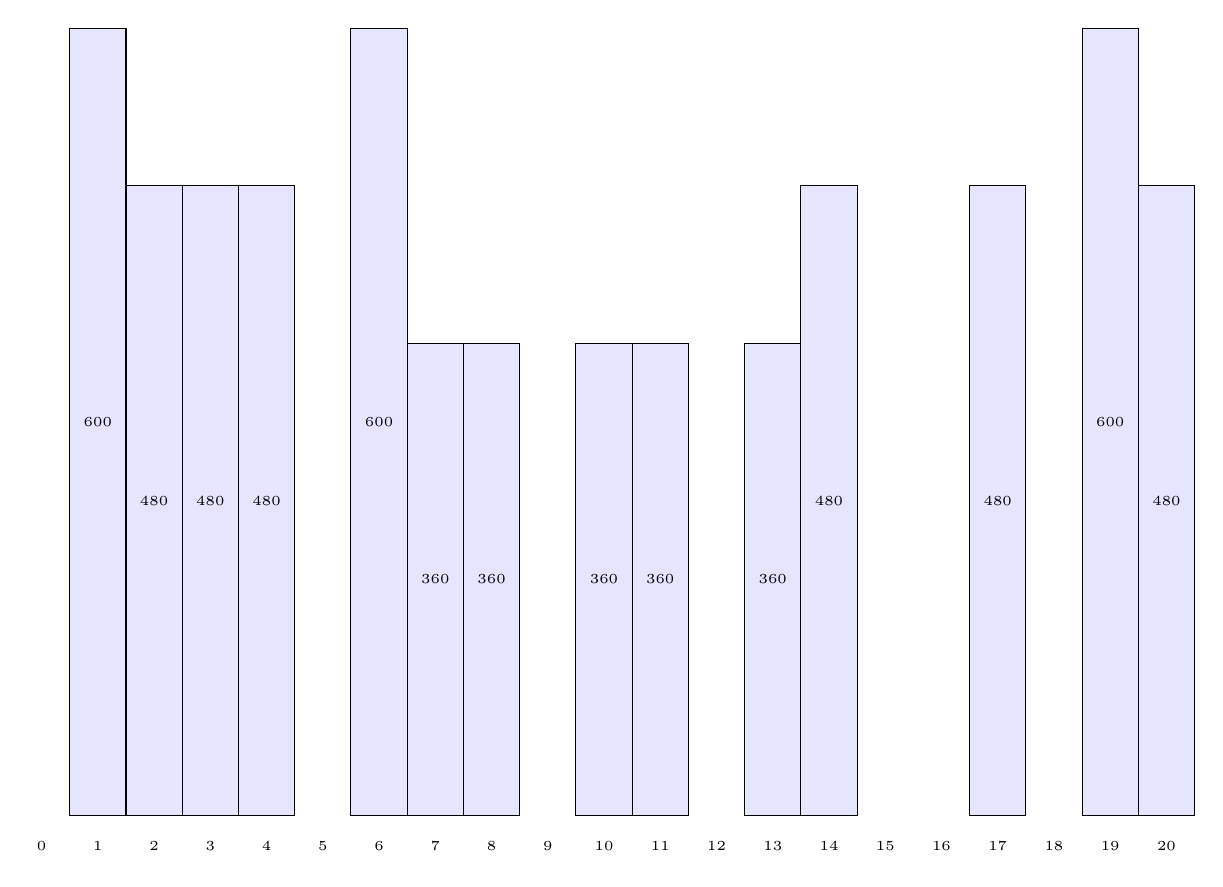
\begin{tikzpicture}[xscale=1.000000,yscale=1.000000]
\node[below] () at (0.357143,-0.2) {\tiny 0};
\node[below] () at (1.071429,-0.2) {\tiny 1};
\node[below] () at (1.785714,-0.2) {\tiny 2};
\node[below] () at (2.500000,-0.2) {\tiny 3};
\node[below] () at (3.214286,-0.2) {\tiny 4};
\node[below] () at (3.928571,-0.2) {\tiny 5};
\node[below] () at (4.642857,-0.2) {\tiny 6};
\node[below] () at (5.357143,-0.2) {\tiny 7};
\node[below] () at (6.071429,-0.2) {\tiny 8};
\node[below] () at (6.785714,-0.2) {\tiny 9};
\node[below] () at (7.500000,-0.2) {\tiny 10};
\node[below] () at (8.214286,-0.2) {\tiny 11};
\node[below] () at (8.928571,-0.2) {\tiny 12};
\node[below] () at (9.642857,-0.2) {\tiny 13};
\node[below] () at (10.357143,-0.2) {\tiny 14};
\node[below] () at (11.071429,-0.2) {\tiny 15};
\node[below] () at (11.785714,-0.2) {\tiny 16};
\node[below] () at (12.500000,-0.2) {\tiny 17};
\node[below] () at (13.214286,-0.2) {\tiny 18};
\node[below] () at (13.928571,-0.2) {\tiny 19};
\node[below] () at (14.642857,-0.2) {\tiny 20};
\draw[draw=black,fill=blue!10] (0.714286,0.000000) rectangle node {\tiny 600} (1.428571,10.000000);
\draw[draw=black,fill=blue!10] (1.428571,0.000000) rectangle node {\tiny 480} (2.142857,8.000000);
\draw[draw=black,fill=blue!10] (2.142857,0.000000) rectangle node {\tiny 480} (2.857143,8.000000);
\draw[draw=black,fill=blue!10] (2.857143,0.000000) rectangle node {\tiny 480} (3.571429,8.000000);
\draw[draw=black,fill=blue!10] (4.285714,0.000000) rectangle node {\tiny 600} (5.000000,10.000000);
\draw[draw=black,fill=blue!10] (5.000000,0.000000) rectangle node {\tiny 360} (5.714286,6.000000);
\draw[draw=black,fill=blue!10] (5.714286,0.000000) rectangle node {\tiny 360} (6.428571,6.000000);
\draw[draw=black,fill=blue!10] (7.142857,0.000000) rectangle node {\tiny 360} (7.857143,6.000000);
\draw[draw=black,fill=blue!10] (7.857143,0.000000) rectangle node {\tiny 360} (8.571429,6.000000);
\draw[draw=black,fill=blue!10] (9.285714,0.000000) rectangle node {\tiny 360} (10.000000,6.000000);
\draw[draw=black,fill=blue!10] (10.000000,0.000000) rectangle node {\tiny 480} (10.714286,8.000000);
\draw[draw=black,fill=blue!10] (12.142857,0.000000) rectangle node {\tiny 480} (12.857143,8.000000);
\draw[draw=black,fill=blue!10] (13.571429,0.000000) rectangle node {\tiny 600} (14.285714,10.000000);
\draw[draw=black,fill=blue!10] (14.285714,0.000000) rectangle node {\tiny 480} (15.000000,8.000000);
\end{tikzpicture}

}
\end{frame}

% \begin{frame}
% \frametitle{Nurses}
% \begin{itemize}
% \item Provide care for patients during their stay
% \item Nurses operate in three non-overlapping shifts
% \item Roster given
% \item Nurses are assigned rooms, responsible for patients in those rooms
% \item Given skill, max workload per shift: soft constraints
% \end{itemize}
% \end{frame}

\begin{frame}[fragile]
\frametitle{Nurse Roster (Part I) - test10}
\scalebox{0.6}{
{\scriptsize
\begin{tabular}{l*{21}{r}} \toprule
& 0& 1& 2& 3& 4& 5& 6& 7& 8& 9& 10& 11& 12& 13& 14& 15& 16& 17& 18& 19& 20\\ \midrule 
n000& L& L& N& & E& L& N& & E& L& N& N& N& N& N& N& N& & E& & E\\ 
n001& L& L& L& L& L& L& & E& L& L& L& L& L& L& L& & E& E& & E& E\\ 
n002& E& & E& L& L& L& L& N& N& N& & E& & E& E& E& L& & E& E& E\\ 
n003& N& N& & E& L& N& N& & E& E& N& & E& E& L& N& & L& L& & E\\ 
n004& L& L& L& N& N& N& N& & L& L& N& N& N& N& & L& L& L& L& L& N\\ 
n005& L& L& L& N& N& & L& N& & N& & L& L& & L& L& L& L& N& N& N\\ 
n006& E& E& L& L& L& N& N& & E& E& L& & E& N& & E& E& E& E& E& E\\ 
n007& L& L& N& & E& E& E& E& E& L& L& & E& E& N& N& N& N& N& & E\\ 
n008& L& L& L& N& & E& L& L& L& & L& L& L& N& N& N& & L& & L& L\\ 
n009& N& N& N& & E& L& L& L& L& & E& L& L& L& N& N& N& & N& & E\\ 
n010& L& N& & E& L& L& L& N& & L& N& N& N& & E& E& & E& E& E& L\\ 
n011& N& N& & E& E& E& L& L& L& L& N& & E& E& E& E& L& L& L& & E\\ 
n012& L& & E& E& E& E& E& E& N& & & E& L& L& & E& E& L& N& N& N\\ 
n013& L& N& & E& L& L& L& & E& L& L& L& L& L& L& & E& N& N& & E\\ 
n014& L& N& N& & L& N& & E& E& L& L& L& N& N& & E& E& N& & E& L\\ 
n015& N& N& N& & L& L& L& L& N& N& & E& L& L& L& L& & E& E& L& L\\ 
n016& N& N& N& & N& & E& E& E& L& L& L& L& N& N& & E& E& E& L& N\\ 
n017& N& N& N& N& & E& N& & E& L& N& N& & N& N& N& N& N& N& N& \\ 
n018& L& & L& L& N& & E& E& N& N& N& & L& L& L& L& L& N& & L& L\\ 
n019& L& L& L& L& L& L& L& L& L& L& & E& L& L& L& N& N& & E& E& L\\ 
n020& L& L& L& N& N& & E& E& E& E& E& E& E& L& L& L& L& L& & L& L\\ 
n021& L& N& N& N& & E& E& L& N& N& N& N& N& N& & L& N& N& N& & E\\ 
n022& L& L& L& L& N& & E& E& L& N& & E& E& E& E& N& N& & E& E& E\\ 
n023& L& L& L& N& N& N& N& & E& N& N& N& & E& E& E& E& E& L& N& N\\ 
n024& N& N& N& N& & E& E& E& E& E& E& E& E& L& L& L& L& L& L& L& L\\ 
\bottomrule
\end{tabular}
}

}
\end{frame}

% \begin{frame}[fragile]
% \frametitle{Nurse Max Workload - test10}
% \scalebox{0.6}{
% {\scriptsize
\begin{tabular}{l*{21}{r}} \toprule
& 0& 1& 2& 3& 4& 5& 6& 7& 8& 9& 10& 11& 12& 13& 14& 15& 16& 17& 18& 19& 20\\ \midrule 
n000& 5& 5& 15& & 15& 15& 15& & 15& 5& 5& 15& 15& 15& 15& 15& 5& & 5& & 15\\ 
n001& 15& 15& 15& 15& 15& 15& & 15& 15& 5& 5& 15& 15& 15& 15& & 15& 15& & 15& 15\\ 
n002& 10& & 10& 10& 10& 10& 10& 10& 10& 10& & 10& & 10& 10& 10& 10& & 10& 10& 10\\ 
n003& 15& 15& & 15& 5& 5& 15& & 15& 15& 15& & 15& 15& 5& 15& & 15& 15& & 15\\ 
n004& 12& 12& 12& 12& 12& 12& 12& & 12& 12& 12& 12& 12& 12& & 12& 12& 12& 12& 12& 12\\ 
n005& 5& 15& 5& 5& 15& & 15& 15& & 5& & 15& 5& & 15& 15& 15& 15& 5& 15& 15\\ 
n006& 15& 15& 5& 15& 15& 15& 15& & 5& 15& 15& & 15& 15& & 15& 15& 15& 15& 15& 15\\ 
n007& 15& 5& 5& & 15& 5& 15& 15& 15& 15& 15& & 15& 15& 5& 15& 15& 15& 15& & 15\\ 
n008& 12& 12& 12& 12& & 12& 12& 12& 12& & 12& 12& 12& 12& 12& 12& & 12& & 12& 12\\ 
n009& 15& 15& 5& & 15& 5& 15& 15& 15& & 15& 15& 15& 15& 5& 5& 15& & 15& & 15\\ 
n010& 5& 15& & 15& 15& 15& 5& 15& & 15& 15& 5& 15& & 15& 15& & 15& 15& 5& 15\\ 
n011& 15& 15& & 15& 15& 15& 15& 15& 15& 5& 15& & 5& 15& 15& 15& 15& 15& 5& & 5\\ 
n012& 15& & 15& 15& 15& 5& 15& 15& 15& & & 15& 15& 15& & 5& 15& 5& 15& 15& 15\\ 
n013& 10& 10& & 10& 10& 10& 10& & 10& 10& 10& 10& 10& 10& 10& & 10& 10& 10& & 10\\ 
n014& 12& 12& 12& & 12& 12& & 12& 12& 12& 12& 12& 12& 12& & 12& 12& 12& & 12& 12\\ 
n015& 5& 15& 15& & 15& 5& 5& 15& 15& 15& & 15& 15& 15& 15& 15& & 15& 5& 15& 5\\ 
n016& 12& 12& 12& & 12& & 12& 12& 12& 12& 12& 12& 12& 12& 12& & 12& 12& 12& 12& 12\\ 
n017& 5& 15& 15& 15& & 5& 15& & 5& 15& 15& 5& & 15& 5& 5& 15& 15& 15& 5& \\ 
n018& 10& & 10& 10& 10& & 10& 10& 10& 10& 10& & 10& 10& 10& 10& 10& 10& & 10& 10\\ 
n019& 15& 15& 15& 15& 5& 15& 5& 15& 15& 15& & 15& 15& 15& 15& 15& 15& & 15& 15& 15\\ 
n020& 10& 10& 10& 10& 10& & 10& 10& 10& 10& 10& 10& 10& 10& 10& 10& 10& 10& & 10& 10\\ 
n021& 12& 12& 12& 12& & 12& 12& 12& 12& 12& 12& 12& 12& 12& & 12& 12& 12& 12& & 12\\ 
n022& 12& 12& 12& 12& 12& & 12& 12& 12& 12& & 12& 12& 12& 12& 12& 12& & 12& 12& 12\\ 
n023& 15& 15& 15& 15& 5& 15& 15& & 15& 15& 5& 5& & 15& 15& 15& 15& 15& 5& 15& 5\\ 
n024& 15& 15& 15& 5& & 5& 15& 15& 5& 15& 5& 15& 15& 5& 15& 15& 5& 15& 15& 15& 5\\ 
\bottomrule
\end{tabular}
}

% }
% \end{frame}
 
 
% \begin{frame}
% \frametitle{Theatres}
% \begin{itemize}
% \item Used for procedures by surgeons
% \item All procedures can be performed in all theatres
% \item Limited total availability per day
% \item Cost, when used, per day
% \item Convenience cost if surgeon assigned to two or more theatres per day
% \end{itemize}
% \end{frame}

% \begin{frame}[fragile]
% \frametitle{Theatre t06 Availability - test10}
% \scalebox{0.6}{
% 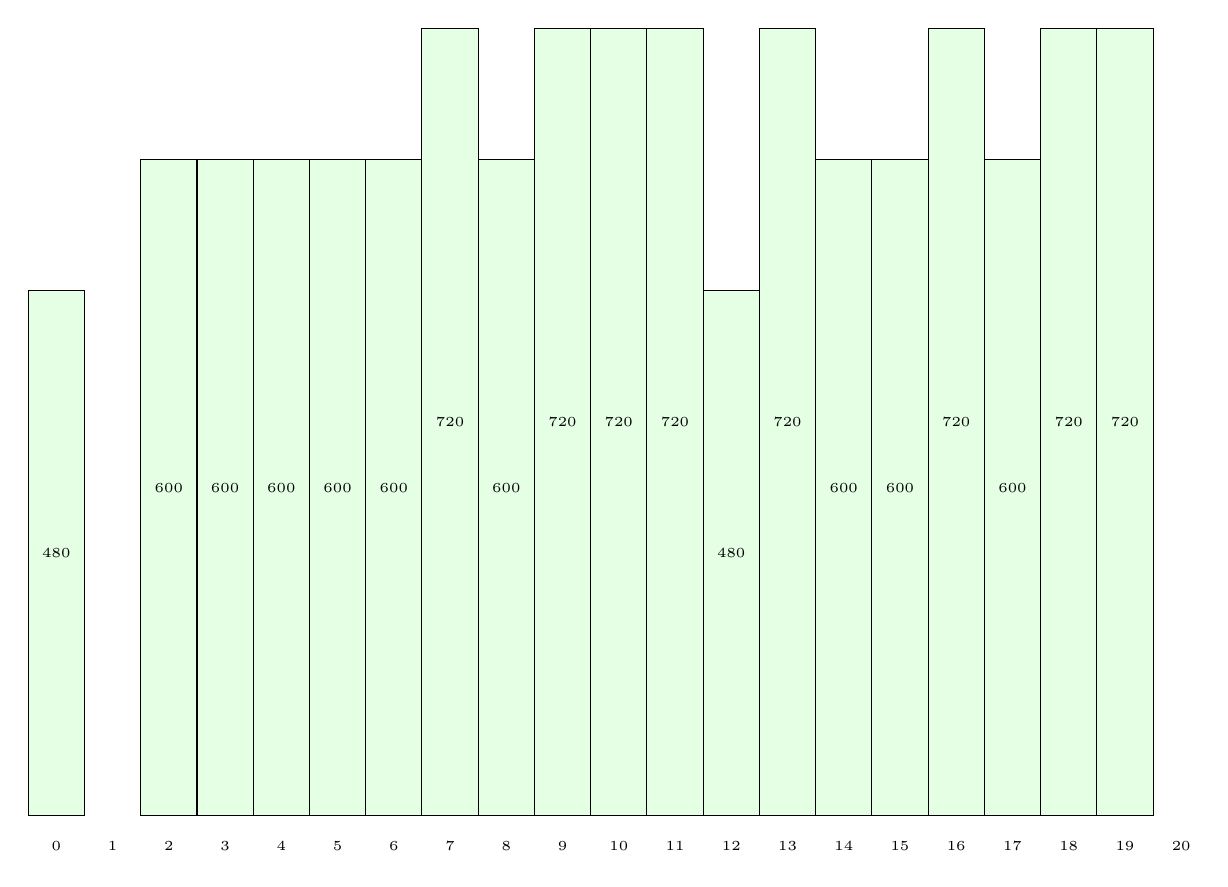
\begin{tikzpicture}[xscale=1.000000,yscale=1.000000]
\node[below] () at (0.357143,-0.2) {\tiny 0};
\node[below] () at (1.071429,-0.2) {\tiny 1};
\node[below] () at (1.785714,-0.2) {\tiny 2};
\node[below] () at (2.500000,-0.2) {\tiny 3};
\node[below] () at (3.214286,-0.2) {\tiny 4};
\node[below] () at (3.928571,-0.2) {\tiny 5};
\node[below] () at (4.642857,-0.2) {\tiny 6};
\node[below] () at (5.357143,-0.2) {\tiny 7};
\node[below] () at (6.071429,-0.2) {\tiny 8};
\node[below] () at (6.785714,-0.2) {\tiny 9};
\node[below] () at (7.500000,-0.2) {\tiny 10};
\node[below] () at (8.214286,-0.2) {\tiny 11};
\node[below] () at (8.928571,-0.2) {\tiny 12};
\node[below] () at (9.642857,-0.2) {\tiny 13};
\node[below] () at (10.357143,-0.2) {\tiny 14};
\node[below] () at (11.071429,-0.2) {\tiny 15};
\node[below] () at (11.785714,-0.2) {\tiny 16};
\node[below] () at (12.500000,-0.2) {\tiny 17};
\node[below] () at (13.214286,-0.2) {\tiny 18};
\node[below] () at (13.928571,-0.2) {\tiny 19};
\node[below] () at (14.642857,-0.2) {\tiny 20};
\draw[draw=black,fill=green!10] (0.000000,0.000000) rectangle node {\tiny 480} (0.714286,6.666667);
\draw[draw=black,fill=green!10] (1.428571,0.000000) rectangle node {\tiny 600} (2.142857,8.333333);
\draw[draw=black,fill=green!10] (2.142857,0.000000) rectangle node {\tiny 600} (2.857143,8.333333);
\draw[draw=black,fill=green!10] (2.857143,0.000000) rectangle node {\tiny 600} (3.571429,8.333333);
\draw[draw=black,fill=green!10] (3.571429,0.000000) rectangle node {\tiny 600} (4.285714,8.333333);
\draw[draw=black,fill=green!10] (4.285714,0.000000) rectangle node {\tiny 600} (5.000000,8.333333);
\draw[draw=black,fill=green!10] (5.000000,0.000000) rectangle node {\tiny 720} (5.714286,10.000000);
\draw[draw=black,fill=green!10] (5.714286,0.000000) rectangle node {\tiny 600} (6.428571,8.333333);
\draw[draw=black,fill=green!10] (6.428571,0.000000) rectangle node {\tiny 720} (7.142857,10.000000);
\draw[draw=black,fill=green!10] (7.142857,0.000000) rectangle node {\tiny 720} (7.857143,10.000000);
\draw[draw=black,fill=green!10] (7.857143,0.000000) rectangle node {\tiny 720} (8.571429,10.000000);
\draw[draw=black,fill=green!10] (8.571429,0.000000) rectangle node {\tiny 480} (9.285714,6.666667);
\draw[draw=black,fill=green!10] (9.285714,0.000000) rectangle node {\tiny 720} (10.000000,10.000000);
\draw[draw=black,fill=green!10] (10.000000,0.000000) rectangle node {\tiny 600} (10.714286,8.333333);
\draw[draw=black,fill=green!10] (10.714286,0.000000) rectangle node {\tiny 600} (11.428571,8.333333);
\draw[draw=black,fill=green!10] (11.428571,0.000000) rectangle node {\tiny 720} (12.142857,10.000000);
\draw[draw=black,fill=green!10] (12.142857,0.000000) rectangle node {\tiny 600} (12.857143,8.333333);
\draw[draw=black,fill=green!10] (12.857143,0.000000) rectangle node {\tiny 720} (13.571429,10.000000);
\draw[draw=black,fill=green!10] (13.571429,0.000000) rectangle node {\tiny 720} (14.285714,10.000000);
\end{tikzpicture}

% }
% \end{frame}

% \begin{frame}
% \frametitle{Rooms/Beds}
% \begin{itemize}
% \item Each patient is assigned a bed in one room during their stay
% \item Each room has a given bed capacity
% \item Rooms/beds are assigned by day
% \item Patients are not moved between rooms
% \item Not all rooms are compatible with all patients
% \item On any day, only patients with same gender can be assigned to the same room, hard constraint
% \item Prefer to have same age-group in the same room, soft constraints
% \end{itemize}
% \end{frame}

\begin{frame}
\frametitle{Weight Factors}
\begin{description}
\item[$w_{u}$] cost of an unscheduled optional patient, i.e. the patient is not admitted in the planning period
\item[$w_{l}$] cost of delay per day for admitting a patient after their release date
\item[$w_{t}$] cost of opening a operating theatre for one day
\item[$w_{s}$] cost of each additional theatre if a surgeon is allocated to more than one theatre per day
\item[$w_{w}$] cost of a workload excess for a nurse in one shift per workload unit
\item[$w_{k}$] cost of skill excess for a nurse in one shift per skill unit
\item[$w_{a}$] cost of a age group conflict between two patients in the same room per day
\item[$w_{c}$] cost of continuity of care excess if multiple nurses are responsible for a patient
\end{description}
\end{frame}




\subsection{Some Data Analysis}

\begin{frame}
\frametitle{Instance Data}
\scalebox{0.7}{
{\scriptsize
\begin{tabular}{lrrrrrrrrrrrr}\toprule
Name &Day &\shortstack{Skill\\Level} &\shortstack{Shift\\Type} &\shortstack{Age\\Group} &Occ &Pat &\shortstack{Mand\\Pat} &Room &Bed &Thea &Surg &Nurse \\ \midrule
test01&21&3&3&3&7&42&11&5&13&2&1&13\\ 
test02&14&3&3&3&5&37&12&6&16&3&2&17\\ 
test03&14&3&3&3&10&45&12&6&20&2&1&14\\ 
test04&14&3&3&3&7&54&32&8&25&3&2&19\\ 
test05&14&3&3&3&9&62&19&6&19&2&1&15\\ 
test06&14&2&3&2&9&111&50&9&22&3&3&20\\ 
test07&21&5&3&5&13&113&55&9&26&3&2&22\\ 
test08&21&2&3&4&15&173&39&9&27&3&2&21\\ 
test09&21&4&3&2&26&146&88&14&44&2&2&29\\ 
\rowcolor{green!10}test10&21&5&3&3&50&525&349&46&130&11&10&83\\ 
m21&14&3&3&3&13&234&32&21&59&11&9&46\\ 
m22&14&2&3&4&36&244&119&30&89&9&7&62\\ 
m23&14&2&3&3&61&254&71&38&117&14&10&77\\ 
m24&21&4&3&3&59&397&264&39&115&11&8&78\\ 
m25&21&2&3&2&32&412&25&26&75&6&7&54\\ 
m26&28&4&3&5&38&570&247&41&125&6&6&81\\ 
m27&14&5&3&5&47&295&87&36&112&16&11&70\\ 
m28&28&2&3&2&36&611&420&42&124&11&10&84\\ 
\rowcolor{green!10}m29&28&4&3&5&44&631&110&49&144&5&8&96\\ 
m30&21&4&3&4&31&489&267&48&140&8&11&90\\ 
\bottomrule
\end{tabular}
}
}
\end{frame}

% \begin{frame}
% \frametitle{Data KPIs (I)}
% \scalebox{0.65}{
% {\scriptsize
\begin{tabular}{lrrrrrrr}\toprule
Name &\shortstack{Mandatory\\Patient\\Percentage} &\shortstack{Gender A\\Patient\\Percentage} &\shortstack{Implied\\Room\\Gender\\Percentage} &\shortstack{Mandatory\\Theatre\\Percentage} &\shortstack{Max Theatre\\Percentage} &\shortstack{Mandatory\\Op\\Percentage} &\shortstack{Max Op\\Percentage} \\ \midrule
test01&26.19&52.38&100.00& 7.89&29.25&36.93&136.93\\ 
test02&32.43&48.65&83.33&10.49&28.89&29.35&\cellcolor{red!10}80.80\\ 
test03&26.67&60.00&100.00&11.22&39.17&79.17&276.39\\ 
test04&59.26&42.59&75.00&16.63&28.45&56.25&96.25\\ 
test05&30.65&45.16&83.33&18.51&71.56&75.78&\cellcolor{red!10}292.97\\ 
test06&45.05&41.44&100.00&22.66&51.64&50.00&113.92\\ 
test07&48.67&46.02&88.89&27.39&55.70&82.78&168.33\\ 
test08&22.54&52.02&100.00&19.91&73.30&61.26&225.55\\ 
test09&60.27&51.37&92.86&60.05&\cellcolor{red!10}108.29&86.33&155.66\\ 
test10&66.48&52.57&80.43&35.25&55.76&72.71&115.04\\ 
m21&13.68&43.59&47.62& \cellcolor{red!10}5.32&43.42&11.30&92.29\\ 
m22&48.77&45.90&76.67&25.69&52.16&53.32&108.24\\ 
m23&27.95&47.64&92.11& 9.62&36.37&23.66&89.48\\ 
m24&66.50&51.64&94.87&32.52&49.76&81.46&124.64\\ 
m25&\cellcolor{red!10} 6.07&51.21&92.31& 4.71&84.50& 8.12&145.72\\ 
m26&43.33&51.75&73.17&31.22&76.73&57.63&141.65\\ 
m27&29.49&45.42&77.78& 9.96&34.71&23.74&82.73\\ 
m28&\cellcolor{red!10}68.74&48.28&73.81&30.71&45.98&64.71&96.88\\ 
m29&17.43&50.87&69.39&17.13&96.48&23.08&130.01\\ 
m30&54.60&52.76&58.33&45.96&84.35&56.31&103.35\\ 
\bottomrule
\end{tabular}
}
% }
% \end{frame}

% \begin{frame}
% \frametitle{Data KPIs (II)}
% \scalebox{0.7}{
% {\scriptsize
\begin{tabular}{lrrrrrr}
\toprule
Name &\shortstack{Worst\\Mandatory\\Surgeon\\Percentage} &\shortstack{Worst\\Max\\Surgeon\\Percentage} &\shortstack{Required\\Bed\\Percentage} &\shortstack{Max\\Bed\\Percentage} &\shortstack{Required\\Nurse\\Load\\Percentage} &\shortstack{Max\\Nurse\\Load\\Percentage} \\ \midrule
test01&36.93&136.93&32.60&92.31&24.65&71.47\\ 
test02&29.69&102.70&41.96&96.43&31.97&74.84\\ 
test03&79.17&276.39&27.14&80.71&26.37&80.99\\ 
test04&58.62&106.90&47.71&79.43&48.98&80.77\\ 
test05&75.78&\cellcolor{red!10}292.97&41.35&122.56&39.69&123.61\\ 
test06&59.46&124.32&\cellcolor{red!10}80.52&\cellcolor{red!10}170.45&\cellcolor{red!10}65.10&140.17\\ 
test07&84.88&169.77&59.71&117.40&54.32&107.78\\ 
test08&63.68&243.42&43.39&153.09&43.78&\cellcolor{red!10}154.31\\ 
test09&81.17&164.17&59.09&92.64&60.32&95.78\\ 
test10&82.74&141.92&64.40&94.40&62.71&92.29\\ 
m21&21.43&152.78&23.37&137.89&21.76&131.94\\ 
m22&64.44&128.91&51.44&96.95&51.06&97.58\\ 
m23&41.48&172.73&28.39&80.71&28.99&85.13\\ 
m24&\cellcolor{red!10}87.26&149.50&58.63&84.51&59.74&86.27\\ 
m25&19.09&230.50&12.44&132.63&11.75&132.31\\ 
m26&66.22&209.50&35.54&77.20&37.71&82.00\\ 
m27&38.24&115.63&34.63&96.94&35.58&103.93\\ 
m28&79.29&119.29&55.79&81.02&57.22&83.34\\ 
m29&27.54&156.64&14.91&73.19&14.82&75.19\\ 
m30&65.35&133.54&46.84&83.61&47.55&85.85\\ 
\bottomrule
\end{tabular}
}
% }
% \end{frame}

% \begin{frame}
% \frametitle{Weight Factors per Instance}
% \scalebox{0.7}{
% {\scriptsize
\begin{tabular}{lrrrrrrrr}\toprule
Name &\shortstack{Room\\Mixed\\Age} &\shortstack{Room\\Nurse\\Skill} &\shortstack{Continuity\\of Care} &\shortstack{Nurse\\Excessive\\Workload} &\shortstack{Open\\Operating\\Theatre} &\shortstack{Surgeon\\Transfer} &\shortstack{Patient\\Delay} &\shortstack{Unscheduled\\Optional} \\ \midrule
test01&5&1&5&1&30&1&5&150\\ 
test02&5&1&1&1&10&10&5&350\\ 
test03&1&1&5&10&10&5&15&350\\ 
test04&1&5&1&5&10&1&10&250\\ 
test05&5&1&5&1&30&10&5&400\\ 
test06&5&1&5&1&30&10&10&500\\ 
test07&5&10&5&1&50&10&5&250\\ 
test08&1&5&1&1&40&1&10&250\\ 
test09&1&5&5&5&20&5&10&350\\ 
\rowcolor{green!10}test10&1&10&5&5&50&10&10&300\\ 
m21&1&5&1&5&40&5&15&500\\ 
m22&5&10&5&5&20&1&10&400\\ 
m23&5&1&5&1&40&10&10&300\\ 
m24&5&10&1&1&20&10&15&350\\ 
m25&1&1&1&1&20&1&10&200\\ 
m26&1&10&1&10&30&10&10&450\\ 
m27&5&5&5&10&40&1&15&150\\ 
m28&1&5&5&5&40&10&10&350\\ 
\rowcolor{green!10}m29&5&10&1&5&50&10&15&150\\ 
m30&5&5&1&1&50&10&10&400\\ 
\bottomrule
\end{tabular}

}
% }
% \end{frame}

\begin{frame}
\frametitle{Total Theatre and Surgeon Capacity - test10}
\scalebox{0.6}{
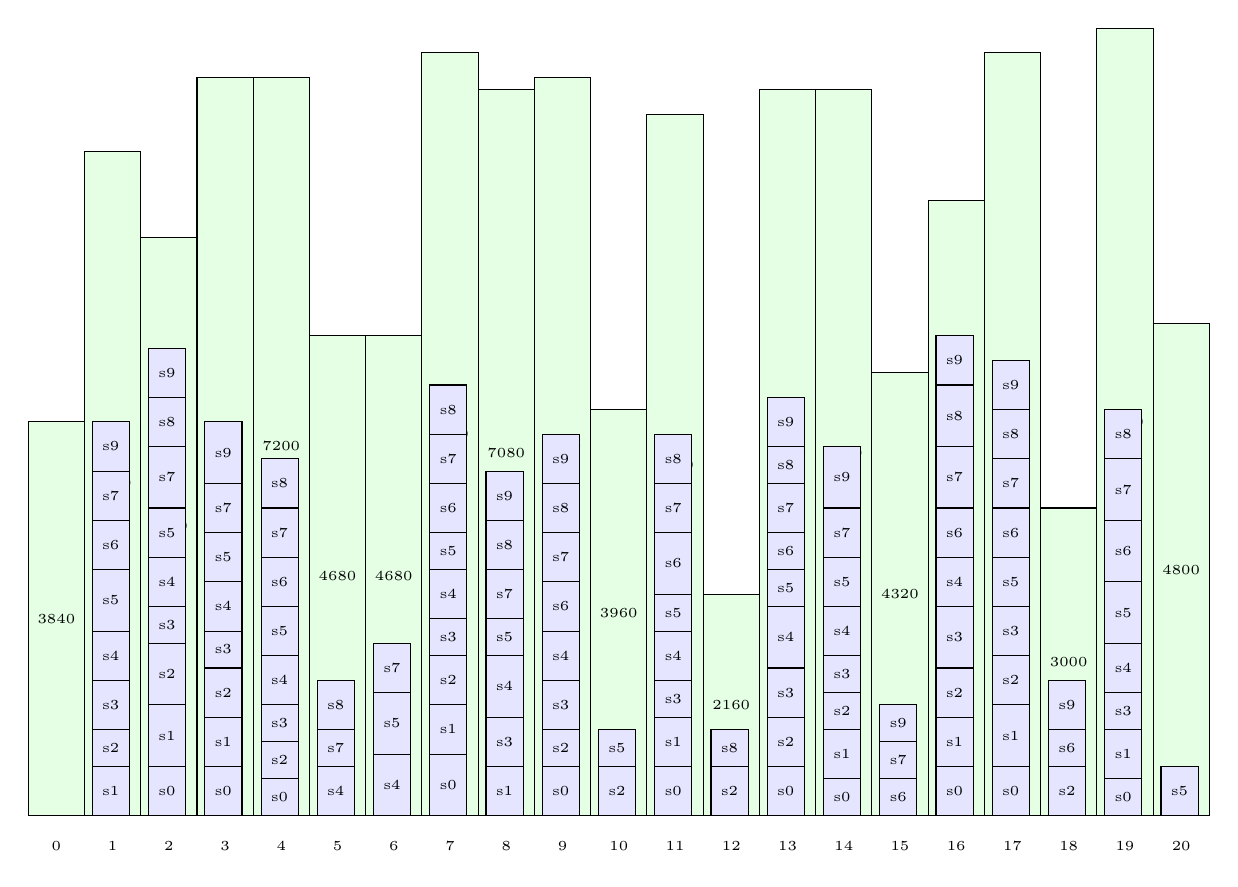
\begin{tikzpicture}[xscale=1.000000,yscale=1.000000]
\node[below] () at (0.357143,-0.2) {\tiny 0};
\node[below] () at (1.071429,-0.2) {\tiny 1};
\node[below] () at (1.785714,-0.2) {\tiny 2};
\node[below] () at (2.500000,-0.2) {\tiny 3};
\node[below] () at (3.214286,-0.2) {\tiny 4};
\node[below] () at (3.928571,-0.2) {\tiny 5};
\node[below] () at (4.642857,-0.2) {\tiny 6};
\node[below] () at (5.357143,-0.2) {\tiny 7};
\node[below] () at (6.071429,-0.2) {\tiny 8};
\node[below] () at (6.785714,-0.2) {\tiny 9};
\node[below] () at (7.500000,-0.2) {\tiny 10};
\node[below] () at (8.214286,-0.2) {\tiny 11};
\node[below] () at (8.928571,-0.2) {\tiny 12};
\node[below] () at (9.642857,-0.2) {\tiny 13};
\node[below] () at (10.357143,-0.2) {\tiny 14};
\node[below] () at (11.071429,-0.2) {\tiny 15};
\node[below] () at (11.785714,-0.2) {\tiny 16};
\node[below] () at (12.500000,-0.2) {\tiny 17};
\node[below] () at (13.214286,-0.2) {\tiny 18};
\node[below] () at (13.928571,-0.2) {\tiny 19};
\node[below] () at (14.642857,-0.2) {\tiny 20};
\draw[draw=black,fill=green!10] (0.000000,0.000000) rectangle node {\tiny 3840} (0.714286,5.000000);
\draw[draw=black,fill=green!10] (0.714286,0.000000) rectangle node {\tiny 6480} (1.428571,8.437500);
\draw[draw=black,fill=blue!10] (0.814286,0.000000) rectangle node {\tiny s1} (1.285714,0.625000);
\draw[draw=black,fill=blue!10] (0.814286,0.625000) rectangle node {\tiny s2} (1.285714,1.093750);
\draw[draw=black,fill=blue!10] (0.814286,1.093750) rectangle node {\tiny s3} (1.285714,1.718750);
\draw[draw=black,fill=blue!10] (0.814286,1.718750) rectangle node {\tiny s4} (1.285714,2.343750);
\draw[draw=black,fill=blue!10] (0.814286,2.343750) rectangle node {\tiny s5} (1.285714,3.125000);
\draw[draw=black,fill=blue!10] (0.814286,3.125000) rectangle node {\tiny s6} (1.285714,3.750000);
\draw[draw=black,fill=blue!10] (0.814286,3.750000) rectangle node {\tiny s7} (1.285714,4.375000);
\draw[draw=black,fill=blue!10] (0.814286,4.375000) rectangle node {\tiny s9} (1.285714,5.000000);
\draw[draw=black,fill=green!10] (1.428571,0.000000) rectangle node {\tiny 5640} (2.142857,7.343750);
\draw[draw=black,fill=blue!10] (1.528571,0.000000) rectangle node {\tiny s0} (2.000000,0.625000);
\draw[draw=black,fill=blue!10] (1.528571,0.625000) rectangle node {\tiny s1} (2.000000,1.406250);
\draw[draw=black,fill=blue!10] (1.528571,1.406250) rectangle node {\tiny s2} (2.000000,2.187500);
\draw[draw=black,fill=blue!10] (1.528571,2.187500) rectangle node {\tiny s3} (2.000000,2.656250);
\draw[draw=black,fill=blue!10] (1.528571,2.656250) rectangle node {\tiny s4} (2.000000,3.281250);
\draw[draw=black,fill=blue!10] (1.528571,3.281250) rectangle node {\tiny s5} (2.000000,3.906250);
\draw[draw=black,fill=blue!10] (1.528571,3.906250) rectangle node {\tiny s7} (2.000000,4.687500);
\draw[draw=black,fill=blue!10] (1.528571,4.687500) rectangle node {\tiny s8} (2.000000,5.312500);
\draw[draw=black,fill=blue!10] (1.528571,5.312500) rectangle node {\tiny s9} (2.000000,5.937500);
\draw[draw=black,fill=green!10] (2.142857,0.000000) rectangle node {\tiny 7200} (2.857143,9.375000);
\draw[draw=black,fill=blue!10] (2.242857,0.000000) rectangle node {\tiny s0} (2.714286,0.625000);
\draw[draw=black,fill=blue!10] (2.242857,0.625000) rectangle node {\tiny s1} (2.714286,1.250000);
\draw[draw=black,fill=blue!10] (2.242857,1.250000) rectangle node {\tiny s2} (2.714286,1.875000);
\draw[draw=black,fill=blue!10] (2.242857,1.875000) rectangle node {\tiny s3} (2.714286,2.343750);
\draw[draw=black,fill=blue!10] (2.242857,2.343750) rectangle node {\tiny s4} (2.714286,2.968750);
\draw[draw=black,fill=blue!10] (2.242857,2.968750) rectangle node {\tiny s5} (2.714286,3.593750);
\draw[draw=black,fill=blue!10] (2.242857,3.593750) rectangle node {\tiny s7} (2.714286,4.218750);
\draw[draw=black,fill=blue!10] (2.242857,4.218750) rectangle node {\tiny s9} (2.714286,5.000000);
\draw[draw=black,fill=green!10] (2.857143,0.000000) rectangle node {\tiny 7200} (3.571429,9.375000);
\draw[draw=black,fill=blue!10] (2.957143,0.000000) rectangle node {\tiny s0} (3.428571,0.468750);
\draw[draw=black,fill=blue!10] (2.957143,0.468750) rectangle node {\tiny s2} (3.428571,0.937500);
\draw[draw=black,fill=blue!10] (2.957143,0.937500) rectangle node {\tiny s3} (3.428571,1.406250);
\draw[draw=black,fill=blue!10] (2.957143,1.406250) rectangle node {\tiny s4} (3.428571,2.031250);
\draw[draw=black,fill=blue!10] (2.957143,2.031250) rectangle node {\tiny s5} (3.428571,2.656250);
\draw[draw=black,fill=blue!10] (2.957143,2.656250) rectangle node {\tiny s6} (3.428571,3.281250);
\draw[draw=black,fill=blue!10] (2.957143,3.281250) rectangle node {\tiny s7} (3.428571,3.906250);
\draw[draw=black,fill=blue!10] (2.957143,3.906250) rectangle node {\tiny s8} (3.428571,4.531250);
\draw[draw=black,fill=green!10] (3.571429,0.000000) rectangle node {\tiny 4680} (4.285714,6.093750);
\draw[draw=black,fill=blue!10] (3.671429,0.000000) rectangle node {\tiny s4} (4.142857,0.625000);
\draw[draw=black,fill=blue!10] (3.671429,0.625000) rectangle node {\tiny s7} (4.142857,1.093750);
\draw[draw=black,fill=blue!10] (3.671429,1.093750) rectangle node {\tiny s8} (4.142857,1.718750);
\draw[draw=black,fill=green!10] (4.285714,0.000000) rectangle node {\tiny 4680} (5.000000,6.093750);
\draw[draw=black,fill=blue!10] (4.385714,0.000000) rectangle node {\tiny s4} (4.857143,0.781250);
\draw[draw=black,fill=blue!10] (4.385714,0.781250) rectangle node {\tiny s5} (4.857143,1.562500);
\draw[draw=black,fill=blue!10] (4.385714,1.562500) rectangle node {\tiny s7} (4.857143,2.187500);
\draw[draw=black,fill=green!10] (5.000000,0.000000) rectangle node {\tiny 7440} (5.714286,9.687500);
\draw[draw=black,fill=blue!10] (5.100000,0.000000) rectangle node {\tiny s0} (5.571429,0.781250);
\draw[draw=black,fill=blue!10] (5.100000,0.781250) rectangle node {\tiny s1} (5.571429,1.406250);
\draw[draw=black,fill=blue!10] (5.100000,1.406250) rectangle node {\tiny s2} (5.571429,2.031250);
\draw[draw=black,fill=blue!10] (5.100000,2.031250) rectangle node {\tiny s3} (5.571429,2.500000);
\draw[draw=black,fill=blue!10] (5.100000,2.500000) rectangle node {\tiny s4} (5.571429,3.125000);
\draw[draw=black,fill=blue!10] (5.100000,3.125000) rectangle node {\tiny s5} (5.571429,3.593750);
\draw[draw=black,fill=blue!10] (5.100000,3.593750) rectangle node {\tiny s6} (5.571429,4.218750);
\draw[draw=black,fill=blue!10] (5.100000,4.218750) rectangle node {\tiny s7} (5.571429,4.843750);
\draw[draw=black,fill=blue!10] (5.100000,4.843750) rectangle node {\tiny s8} (5.571429,5.468750);
\draw[draw=black,fill=green!10] (5.714286,0.000000) rectangle node {\tiny 7080} (6.428571,9.218750);
\draw[draw=black,fill=blue!10] (5.814286,0.000000) rectangle node {\tiny s1} (6.285714,0.625000);
\draw[draw=black,fill=blue!10] (5.814286,0.625000) rectangle node {\tiny s3} (6.285714,1.250000);
\draw[draw=black,fill=blue!10] (5.814286,1.250000) rectangle node {\tiny s4} (6.285714,2.031250);
\draw[draw=black,fill=blue!10] (5.814286,2.031250) rectangle node {\tiny s5} (6.285714,2.500000);
\draw[draw=black,fill=blue!10] (5.814286,2.500000) rectangle node {\tiny s7} (6.285714,3.125000);
\draw[draw=black,fill=blue!10] (5.814286,3.125000) rectangle node {\tiny s8} (6.285714,3.750000);
\draw[draw=black,fill=blue!10] (5.814286,3.750000) rectangle node {\tiny s9} (6.285714,4.375000);
\draw[draw=black,fill=green!10] (6.428571,0.000000) rectangle node {\tiny 7200} (7.142857,9.375000);
\draw[draw=black,fill=blue!10] (6.528571,0.000000) rectangle node {\tiny s0} (7.000000,0.625000);
\draw[draw=black,fill=blue!10] (6.528571,0.625000) rectangle node {\tiny s2} (7.000000,1.093750);
\draw[draw=black,fill=blue!10] (6.528571,1.093750) rectangle node {\tiny s3} (7.000000,1.718750);
\draw[draw=black,fill=blue!10] (6.528571,1.718750) rectangle node {\tiny s4} (7.000000,2.343750);
\draw[draw=black,fill=blue!10] (6.528571,2.343750) rectangle node {\tiny s6} (7.000000,2.968750);
\draw[draw=black,fill=blue!10] (6.528571,2.968750) rectangle node {\tiny s7} (7.000000,3.593750);
\draw[draw=black,fill=blue!10] (6.528571,3.593750) rectangle node {\tiny s8} (7.000000,4.218750);
\draw[draw=black,fill=blue!10] (6.528571,4.218750) rectangle node {\tiny s9} (7.000000,4.843750);
\draw[draw=black,fill=green!10] (7.142857,0.000000) rectangle node {\tiny 3960} (7.857143,5.156250);
\draw[draw=black,fill=blue!10] (7.242857,0.000000) rectangle node {\tiny s2} (7.714286,0.625000);
\draw[draw=black,fill=blue!10] (7.242857,0.625000) rectangle node {\tiny s5} (7.714286,1.093750);
\draw[draw=black,fill=green!10] (7.857143,0.000000) rectangle node {\tiny 6840} (8.571429,8.906250);
\draw[draw=black,fill=blue!10] (7.957143,0.000000) rectangle node {\tiny s0} (8.428571,0.625000);
\draw[draw=black,fill=blue!10] (7.957143,0.625000) rectangle node {\tiny s1} (8.428571,1.250000);
\draw[draw=black,fill=blue!10] (7.957143,1.250000) rectangle node {\tiny s3} (8.428571,1.718750);
\draw[draw=black,fill=blue!10] (7.957143,1.718750) rectangle node {\tiny s4} (8.428571,2.343750);
\draw[draw=black,fill=blue!10] (7.957143,2.343750) rectangle node {\tiny s5} (8.428571,2.812500);
\draw[draw=black,fill=blue!10] (7.957143,2.812500) rectangle node {\tiny s6} (8.428571,3.593750);
\draw[draw=black,fill=blue!10] (7.957143,3.593750) rectangle node {\tiny s7} (8.428571,4.218750);
\draw[draw=black,fill=blue!10] (7.957143,4.218750) rectangle node {\tiny s8} (8.428571,4.843750);
\draw[draw=black,fill=green!10] (8.571429,0.000000) rectangle node {\tiny 2160} (9.285714,2.812500);
\draw[draw=black,fill=blue!10] (8.671429,0.000000) rectangle node {\tiny s2} (9.142857,0.625000);
\draw[draw=black,fill=blue!10] (8.671429,0.625000) rectangle node {\tiny s8} (9.142857,1.093750);
\draw[draw=black,fill=green!10] (9.285714,0.000000) rectangle node {\tiny 7080} (10.000000,9.218750);
\draw[draw=black,fill=blue!10] (9.385714,0.000000) rectangle node {\tiny s0} (9.857143,0.625000);
\draw[draw=black,fill=blue!10] (9.385714,0.625000) rectangle node {\tiny s2} (9.857143,1.250000);
\draw[draw=black,fill=blue!10] (9.385714,1.250000) rectangle node {\tiny s3} (9.857143,1.875000);
\draw[draw=black,fill=blue!10] (9.385714,1.875000) rectangle node {\tiny s4} (9.857143,2.656250);
\draw[draw=black,fill=blue!10] (9.385714,2.656250) rectangle node {\tiny s5} (9.857143,3.125000);
\draw[draw=black,fill=blue!10] (9.385714,3.125000) rectangle node {\tiny s6} (9.857143,3.593750);
\draw[draw=black,fill=blue!10] (9.385714,3.593750) rectangle node {\tiny s7} (9.857143,4.218750);
\draw[draw=black,fill=blue!10] (9.385714,4.218750) rectangle node {\tiny s8} (9.857143,4.687500);
\draw[draw=black,fill=blue!10] (9.385714,4.687500) rectangle node {\tiny s9} (9.857143,5.312500);
\draw[draw=black,fill=green!10] (10.000000,0.000000) rectangle node {\tiny 7080} (10.714286,9.218750);
\draw[draw=black,fill=blue!10] (10.100000,0.000000) rectangle node {\tiny s0} (10.571429,0.468750);
\draw[draw=black,fill=blue!10] (10.100000,0.468750) rectangle node {\tiny s1} (10.571429,1.093750);
\draw[draw=black,fill=blue!10] (10.100000,1.093750) rectangle node {\tiny s2} (10.571429,1.562500);
\draw[draw=black,fill=blue!10] (10.100000,1.562500) rectangle node {\tiny s3} (10.571429,2.031250);
\draw[draw=black,fill=blue!10] (10.100000,2.031250) rectangle node {\tiny s4} (10.571429,2.656250);
\draw[draw=black,fill=blue!10] (10.100000,2.656250) rectangle node {\tiny s5} (10.571429,3.281250);
\draw[draw=black,fill=blue!10] (10.100000,3.281250) rectangle node {\tiny s7} (10.571429,3.906250);
\draw[draw=black,fill=blue!10] (10.100000,3.906250) rectangle node {\tiny s9} (10.571429,4.687500);
\draw[draw=black,fill=green!10] (10.714286,0.000000) rectangle node {\tiny 4320} (11.428571,5.625000);
\draw[draw=black,fill=blue!10] (10.814286,0.000000) rectangle node {\tiny s6} (11.285714,0.468750);
\draw[draw=black,fill=blue!10] (10.814286,0.468750) rectangle node {\tiny s7} (11.285714,0.937500);
\draw[draw=black,fill=blue!10] (10.814286,0.937500) rectangle node {\tiny s9} (11.285714,1.406250);
\draw[draw=black,fill=green!10] (11.428571,0.000000) rectangle node {\tiny 6000} (12.142857,7.812500);
\draw[draw=black,fill=blue!10] (11.528571,0.000000) rectangle node {\tiny s0} (12.000000,0.625000);
\draw[draw=black,fill=blue!10] (11.528571,0.625000) rectangle node {\tiny s1} (12.000000,1.250000);
\draw[draw=black,fill=blue!10] (11.528571,1.250000) rectangle node {\tiny s2} (12.000000,1.875000);
\draw[draw=black,fill=blue!10] (11.528571,1.875000) rectangle node {\tiny s3} (12.000000,2.656250);
\draw[draw=black,fill=blue!10] (11.528571,2.656250) rectangle node {\tiny s4} (12.000000,3.281250);
\draw[draw=black,fill=blue!10] (11.528571,3.281250) rectangle node {\tiny s6} (12.000000,3.906250);
\draw[draw=black,fill=blue!10] (11.528571,3.906250) rectangle node {\tiny s7} (12.000000,4.687500);
\draw[draw=black,fill=blue!10] (11.528571,4.687500) rectangle node {\tiny s8} (12.000000,5.468750);
\draw[draw=black,fill=blue!10] (11.528571,5.468750) rectangle node {\tiny s9} (12.000000,6.093750);
\draw[draw=black,fill=green!10] (12.142857,0.000000) rectangle node {\tiny 7440} (12.857143,9.687500);
\draw[draw=black,fill=blue!10] (12.242857,0.000000) rectangle node {\tiny s0} (12.714286,0.625000);
\draw[draw=black,fill=blue!10] (12.242857,0.625000) rectangle node {\tiny s1} (12.714286,1.406250);
\draw[draw=black,fill=blue!10] (12.242857,1.406250) rectangle node {\tiny s2} (12.714286,2.031250);
\draw[draw=black,fill=blue!10] (12.242857,2.031250) rectangle node {\tiny s3} (12.714286,2.656250);
\draw[draw=black,fill=blue!10] (12.242857,2.656250) rectangle node {\tiny s5} (12.714286,3.281250);
\draw[draw=black,fill=blue!10] (12.242857,3.281250) rectangle node {\tiny s6} (12.714286,3.906250);
\draw[draw=black,fill=blue!10] (12.242857,3.906250) rectangle node {\tiny s7} (12.714286,4.531250);
\draw[draw=black,fill=blue!10] (12.242857,4.531250) rectangle node {\tiny s8} (12.714286,5.156250);
\draw[draw=black,fill=blue!10] (12.242857,5.156250) rectangle node {\tiny s9} (12.714286,5.781250);
\draw[draw=black,fill=green!10] (12.857143,0.000000) rectangle node {\tiny 3000} (13.571429,3.906250);
\draw[draw=black,fill=blue!10] (12.957143,0.000000) rectangle node {\tiny s2} (13.428571,0.625000);
\draw[draw=black,fill=blue!10] (12.957143,0.625000) rectangle node {\tiny s6} (13.428571,1.093750);
\draw[draw=black,fill=blue!10] (12.957143,1.093750) rectangle node {\tiny s9} (13.428571,1.718750);
\draw[draw=black,fill=green!10] (13.571429,0.000000) rectangle node {\tiny 7680} (14.285714,10.000000);
\draw[draw=black,fill=blue!10] (13.671429,0.000000) rectangle node {\tiny s0} (14.142857,0.468750);
\draw[draw=black,fill=blue!10] (13.671429,0.468750) rectangle node {\tiny s1} (14.142857,1.093750);
\draw[draw=black,fill=blue!10] (13.671429,1.093750) rectangle node {\tiny s3} (14.142857,1.562500);
\draw[draw=black,fill=blue!10] (13.671429,1.562500) rectangle node {\tiny s4} (14.142857,2.187500);
\draw[draw=black,fill=blue!10] (13.671429,2.187500) rectangle node {\tiny s5} (14.142857,2.968750);
\draw[draw=black,fill=blue!10] (13.671429,2.968750) rectangle node {\tiny s6} (14.142857,3.750000);
\draw[draw=black,fill=blue!10] (13.671429,3.750000) rectangle node {\tiny s7} (14.142857,4.531250);
\draw[draw=black,fill=blue!10] (13.671429,4.531250) rectangle node {\tiny s8} (14.142857,5.156250);
\draw[draw=black,fill=green!10] (14.285714,0.000000) rectangle node {\tiny 4800} (15.000000,6.250000);
\draw[draw=black,fill=blue!10] (14.385714,0.000000) rectangle node {\tiny s5} (14.857143,0.625000);
\end{tikzpicture}

}
 \begin{textblock}{4}(11,5)
  Theatre capacity not limiting
 \end{textblock}
\end{frame}

\begin{frame}
\frametitle{Total Theatre and Surgeon Capacity - m29}
\scalebox{0.6}{
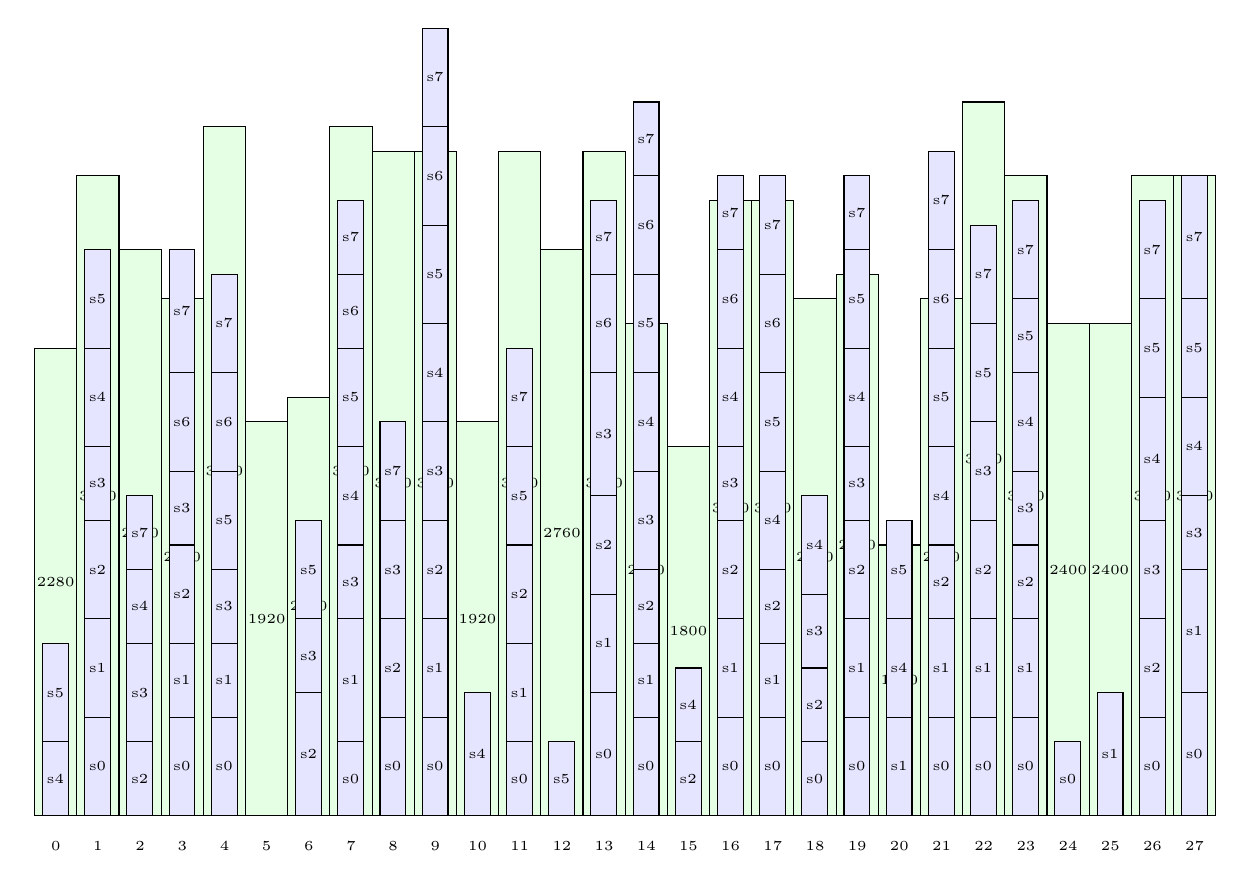
\begin{tikzpicture}[xscale=1.000000,yscale=1.000000]
\node[below] () at (0.267857,-0.2) {\tiny 0};
\node[below] () at (0.803571,-0.2) {\tiny 1};
\node[below] () at (1.339286,-0.2) {\tiny 2};
\node[below] () at (1.875000,-0.2) {\tiny 3};
\node[below] () at (2.410714,-0.2) {\tiny 4};
\node[below] () at (2.946429,-0.2) {\tiny 5};
\node[below] () at (3.482143,-0.2) {\tiny 6};
\node[below] () at (4.017857,-0.2) {\tiny 7};
\node[below] () at (4.553571,-0.2) {\tiny 8};
\node[below] () at (5.089286,-0.2) {\tiny 9};
\node[below] () at (5.625000,-0.2) {\tiny 10};
\node[below] () at (6.160714,-0.2) {\tiny 11};
\node[below] () at (6.696429,-0.2) {\tiny 12};
\node[below] () at (7.232143,-0.2) {\tiny 13};
\node[below] () at (7.767857,-0.2) {\tiny 14};
\node[below] () at (8.303571,-0.2) {\tiny 15};
\node[below] () at (8.839286,-0.2) {\tiny 16};
\node[below] () at (9.375000,-0.2) {\tiny 17};
\node[below] () at (9.910714,-0.2) {\tiny 18};
\node[below] () at (10.446429,-0.2) {\tiny 19};
\node[below] () at (10.982143,-0.2) {\tiny 20};
\node[below] () at (11.517857,-0.2) {\tiny 21};
\node[below] () at (12.053571,-0.2) {\tiny 22};
\node[below] () at (12.589286,-0.2) {\tiny 23};
\node[below] () at (13.125000,-0.2) {\tiny 24};
\node[below] () at (13.660714,-0.2) {\tiny 25};
\node[below] () at (14.196429,-0.2) {\tiny 26};
\node[below] () at (14.732143,-0.2) {\tiny 27};
\draw[draw=black,fill=green!10] (0.000000,0.000000) rectangle node {\tiny 2280} (0.535714,5.937500);
\draw[draw=black,fill=blue!10] (0.100000,0.000000) rectangle node {\tiny s4} (0.428571,0.937500);
\draw[draw=black,fill=blue!10] (0.100000,0.937500) rectangle node {\tiny s5} (0.428571,2.187500);
\draw[draw=black,fill=green!10] (0.535714,0.000000) rectangle node {\tiny 3120} (1.071429,8.125000);
\draw[draw=black,fill=blue!10] (0.635714,0.000000) rectangle node {\tiny s0} (0.964286,1.250000);
\draw[draw=black,fill=blue!10] (0.635714,1.250000) rectangle node {\tiny s1} (0.964286,2.500000);
\draw[draw=black,fill=blue!10] (0.635714,2.500000) rectangle node {\tiny s2} (0.964286,3.750000);
\draw[draw=black,fill=blue!10] (0.635714,3.750000) rectangle node {\tiny s3} (0.964286,4.687500);
\draw[draw=black,fill=blue!10] (0.635714,4.687500) rectangle node {\tiny s4} (0.964286,5.937500);
\draw[draw=black,fill=blue!10] (0.635714,5.937500) rectangle node {\tiny s5} (0.964286,7.187500);
\draw[draw=black,fill=green!10] (1.071429,0.000000) rectangle node {\tiny 2760} (1.607143,7.187500);
\draw[draw=black,fill=blue!10] (1.171429,0.000000) rectangle node {\tiny s2} (1.500000,0.937500);
\draw[draw=black,fill=blue!10] (1.171429,0.937500) rectangle node {\tiny s3} (1.500000,2.187500);
\draw[draw=black,fill=blue!10] (1.171429,2.187500) rectangle node {\tiny s4} (1.500000,3.125000);
\draw[draw=black,fill=blue!10] (1.171429,3.125000) rectangle node {\tiny s7} (1.500000,4.062500);
\draw[draw=black,fill=green!10] (1.607143,0.000000) rectangle node {\tiny 2520} (2.142857,6.562500);
\draw[draw=black,fill=blue!10] (1.707143,0.000000) rectangle node {\tiny s0} (2.035714,1.250000);
\draw[draw=black,fill=blue!10] (1.707143,1.250000) rectangle node {\tiny s1} (2.035714,2.187500);
\draw[draw=black,fill=blue!10] (1.707143,2.187500) rectangle node {\tiny s2} (2.035714,3.437500);
\draw[draw=black,fill=blue!10] (1.707143,3.437500) rectangle node {\tiny s3} (2.035714,4.375000);
\draw[draw=black,fill=blue!10] (1.707143,4.375000) rectangle node {\tiny s6} (2.035714,5.625000);
\draw[draw=black,fill=blue!10] (1.707143,5.625000) rectangle node {\tiny s7} (2.035714,7.187500);
\draw[draw=black,fill=green!10] (2.142857,0.000000) rectangle node {\tiny 3360} (2.678571,8.750000);
\draw[draw=black,fill=blue!10] (2.242857,0.000000) rectangle node {\tiny s0} (2.571429,1.250000);
\draw[draw=black,fill=blue!10] (2.242857,1.250000) rectangle node {\tiny s1} (2.571429,2.187500);
\draw[draw=black,fill=blue!10] (2.242857,2.187500) rectangle node {\tiny s3} (2.571429,3.125000);
\draw[draw=black,fill=blue!10] (2.242857,3.125000) rectangle node {\tiny s5} (2.571429,4.375000);
\draw[draw=black,fill=blue!10] (2.242857,4.375000) rectangle node {\tiny s6} (2.571429,5.625000);
\draw[draw=black,fill=blue!10] (2.242857,5.625000) rectangle node {\tiny s7} (2.571429,6.875000);
\draw[draw=black,fill=green!10] (2.678571,0.000000) rectangle node {\tiny 1920} (3.214286,5.000000);
\draw[draw=black,fill=green!10] (3.214286,0.000000) rectangle node {\tiny 2040} (3.750000,5.312500);
\draw[draw=black,fill=blue!10] (3.314286,0.000000) rectangle node {\tiny s2} (3.642857,1.562500);
\draw[draw=black,fill=blue!10] (3.314286,1.562500) rectangle node {\tiny s3} (3.642857,2.500000);
\draw[draw=black,fill=blue!10] (3.314286,2.500000) rectangle node {\tiny s5} (3.642857,3.750000);
\draw[draw=black,fill=green!10] (3.750000,0.000000) rectangle node {\tiny 3360} (4.285714,8.750000);
\draw[draw=black,fill=blue!10] (3.850000,0.000000) rectangle node {\tiny s0} (4.178571,0.937500);
\draw[draw=black,fill=blue!10] (3.850000,0.937500) rectangle node {\tiny s1} (4.178571,2.500000);
\draw[draw=black,fill=blue!10] (3.850000,2.500000) rectangle node {\tiny s3} (4.178571,3.437500);
\draw[draw=black,fill=blue!10] (3.850000,3.437500) rectangle node {\tiny s4} (4.178571,4.687500);
\draw[draw=black,fill=blue!10] (3.850000,4.687500) rectangle node {\tiny s5} (4.178571,5.937500);
\draw[draw=black,fill=blue!10] (3.850000,5.937500) rectangle node {\tiny s6} (4.178571,6.875000);
\draw[draw=black,fill=blue!10] (3.850000,6.875000) rectangle node {\tiny s7} (4.178571,7.812500);
\draw[draw=black,fill=green!10] (4.285714,0.000000) rectangle node {\tiny 3240} (4.821429,8.437500);
\draw[draw=black,fill=blue!10] (4.385714,0.000000) rectangle node {\tiny s0} (4.714286,1.250000);
\draw[draw=black,fill=blue!10] (4.385714,1.250000) rectangle node {\tiny s2} (4.714286,2.500000);
\draw[draw=black,fill=blue!10] (4.385714,2.500000) rectangle node {\tiny s3} (4.714286,3.750000);
\draw[draw=black,fill=blue!10] (4.385714,3.750000) rectangle node {\tiny s7} (4.714286,5.000000);
\draw[draw=black,fill=green!10] (4.821429,0.000000) rectangle node {\tiny 3240} (5.357143,8.437500);
\draw[draw=black,fill=blue!10] (4.921429,0.000000) rectangle node {\tiny s0} (5.250000,1.250000);
\draw[draw=black,fill=blue!10] (4.921429,1.250000) rectangle node {\tiny s1} (5.250000,2.500000);
\draw[draw=black,fill=blue!10] (4.921429,2.500000) rectangle node {\tiny s2} (5.250000,3.750000);
\draw[draw=black,fill=blue!10] (4.921429,3.750000) rectangle node {\tiny s3} (5.250000,5.000000);
\draw[draw=black,fill=blue!10] (4.921429,5.000000) rectangle node {\tiny s4} (5.250000,6.250000);
\draw[draw=black,fill=blue!10] (4.921429,6.250000) rectangle node {\tiny s5} (5.250000,7.500000);
\draw[draw=black,fill=blue!10] (4.921429,7.500000) rectangle node {\tiny s6} (5.250000,8.750000);
\draw[draw=black,fill=blue!10] (4.921429,8.750000) rectangle node {\tiny s7} (5.250000,10.000000);
\draw[draw=black,fill=green!10] (5.357143,0.000000) rectangle node {\tiny 1920} (5.892857,5.000000);
\draw[draw=black,fill=blue!10] (5.457143,0.000000) rectangle node {\tiny s4} (5.785714,1.562500);
\draw[draw=black,fill=green!10] (5.892857,0.000000) rectangle node {\tiny 3240} (6.428571,8.437500);
\draw[draw=black,fill=blue!10] (5.992857,0.000000) rectangle node {\tiny s0} (6.321429,0.937500);
\draw[draw=black,fill=blue!10] (5.992857,0.937500) rectangle node {\tiny s1} (6.321429,2.187500);
\draw[draw=black,fill=blue!10] (5.992857,2.187500) rectangle node {\tiny s2} (6.321429,3.437500);
\draw[draw=black,fill=blue!10] (5.992857,3.437500) rectangle node {\tiny s5} (6.321429,4.687500);
\draw[draw=black,fill=blue!10] (5.992857,4.687500) rectangle node {\tiny s7} (6.321429,5.937500);
\draw[draw=black,fill=green!10] (6.428571,0.000000) rectangle node {\tiny 2760} (6.964286,7.187500);
\draw[draw=black,fill=blue!10] (6.528571,0.000000) rectangle node {\tiny s5} (6.857143,0.937500);
\draw[draw=black,fill=green!10] (6.964286,0.000000) rectangle node {\tiny 3240} (7.500000,8.437500);
\draw[draw=black,fill=blue!10] (7.064286,0.000000) rectangle node {\tiny s0} (7.392857,1.562500);
\draw[draw=black,fill=blue!10] (7.064286,1.562500) rectangle node {\tiny s1} (7.392857,2.812500);
\draw[draw=black,fill=blue!10] (7.064286,2.812500) rectangle node {\tiny s2} (7.392857,4.062500);
\draw[draw=black,fill=blue!10] (7.064286,4.062500) rectangle node {\tiny s3} (7.392857,5.625000);
\draw[draw=black,fill=blue!10] (7.064286,5.625000) rectangle node {\tiny s6} (7.392857,6.875000);
\draw[draw=black,fill=blue!10] (7.064286,6.875000) rectangle node {\tiny s7} (7.392857,7.812500);
\draw[draw=black,fill=green!10] (7.500000,0.000000) rectangle node {\tiny 2400} (8.035714,6.250000);
\draw[draw=black,fill=blue!10] (7.600000,0.000000) rectangle node {\tiny s0} (7.928571,1.250000);
\draw[draw=black,fill=blue!10] (7.600000,1.250000) rectangle node {\tiny s1} (7.928571,2.187500);
\draw[draw=black,fill=blue!10] (7.600000,2.187500) rectangle node {\tiny s2} (7.928571,3.125000);
\draw[draw=black,fill=blue!10] (7.600000,3.125000) rectangle node {\tiny s3} (7.928571,4.375000);
\draw[draw=black,fill=blue!10] (7.600000,4.375000) rectangle node {\tiny s4} (7.928571,5.625000);
\draw[draw=black,fill=blue!10] (7.600000,5.625000) rectangle node {\tiny s5} (7.928571,6.875000);
\draw[draw=black,fill=blue!10] (7.600000,6.875000) rectangle node {\tiny s6} (7.928571,8.125000);
\draw[draw=black,fill=blue!10] (7.600000,8.125000) rectangle node {\tiny s7} (7.928571,9.062500);
\draw[draw=black,fill=green!10] (8.035714,0.000000) rectangle node {\tiny 1800} (8.571429,4.687500);
\draw[draw=black,fill=blue!10] (8.135714,0.000000) rectangle node {\tiny s2} (8.464286,0.937500);
\draw[draw=black,fill=blue!10] (8.135714,0.937500) rectangle node {\tiny s4} (8.464286,1.875000);
\draw[draw=black,fill=green!10] (8.571429,0.000000) rectangle node {\tiny 3000} (9.107143,7.812500);
\draw[draw=black,fill=blue!10] (8.671429,0.000000) rectangle node {\tiny s0} (9.000000,1.250000);
\draw[draw=black,fill=blue!10] (8.671429,1.250000) rectangle node {\tiny s1} (9.000000,2.500000);
\draw[draw=black,fill=blue!10] (8.671429,2.500000) rectangle node {\tiny s2} (9.000000,3.750000);
\draw[draw=black,fill=blue!10] (8.671429,3.750000) rectangle node {\tiny s3} (9.000000,4.687500);
\draw[draw=black,fill=blue!10] (8.671429,4.687500) rectangle node {\tiny s4} (9.000000,5.937500);
\draw[draw=black,fill=blue!10] (8.671429,5.937500) rectangle node {\tiny s6} (9.000000,7.187500);
\draw[draw=black,fill=blue!10] (8.671429,7.187500) rectangle node {\tiny s7} (9.000000,8.125000);
\draw[draw=black,fill=green!10] (9.107143,0.000000) rectangle node {\tiny 3000} (9.642857,7.812500);
\draw[draw=black,fill=blue!10] (9.207143,0.000000) rectangle node {\tiny s0} (9.535714,1.250000);
\draw[draw=black,fill=blue!10] (9.207143,1.250000) rectangle node {\tiny s1} (9.535714,2.187500);
\draw[draw=black,fill=blue!10] (9.207143,2.187500) rectangle node {\tiny s2} (9.535714,3.125000);
\draw[draw=black,fill=blue!10] (9.207143,3.125000) rectangle node {\tiny s4} (9.535714,4.375000);
\draw[draw=black,fill=blue!10] (9.207143,4.375000) rectangle node {\tiny s5} (9.535714,5.625000);
\draw[draw=black,fill=blue!10] (9.207143,5.625000) rectangle node {\tiny s6} (9.535714,6.875000);
\draw[draw=black,fill=blue!10] (9.207143,6.875000) rectangle node {\tiny s7} (9.535714,8.125000);
\draw[draw=black,fill=green!10] (9.642857,0.000000) rectangle node {\tiny 2520} (10.178571,6.562500);
\draw[draw=black,fill=blue!10] (9.742857,0.000000) rectangle node {\tiny s0} (10.071429,0.937500);
\draw[draw=black,fill=blue!10] (9.742857,0.937500) rectangle node {\tiny s2} (10.071429,1.875000);
\draw[draw=black,fill=blue!10] (9.742857,1.875000) rectangle node {\tiny s3} (10.071429,2.812500);
\draw[draw=black,fill=blue!10] (9.742857,2.812500) rectangle node {\tiny s4} (10.071429,4.062500);
\draw[draw=black,fill=green!10] (10.178571,0.000000) rectangle node {\tiny 2640} (10.714286,6.875000);
\draw[draw=black,fill=blue!10] (10.278571,0.000000) rectangle node {\tiny s0} (10.607143,1.250000);
\draw[draw=black,fill=blue!10] (10.278571,1.250000) rectangle node {\tiny s1} (10.607143,2.500000);
\draw[draw=black,fill=blue!10] (10.278571,2.500000) rectangle node {\tiny s2} (10.607143,3.750000);
\draw[draw=black,fill=blue!10] (10.278571,3.750000) rectangle node {\tiny s3} (10.607143,4.687500);
\draw[draw=black,fill=blue!10] (10.278571,4.687500) rectangle node {\tiny s4} (10.607143,5.937500);
\draw[draw=black,fill=blue!10] (10.278571,5.937500) rectangle node {\tiny s5} (10.607143,7.187500);
\draw[draw=black,fill=blue!10] (10.278571,7.187500) rectangle node {\tiny s7} (10.607143,8.125000);
\draw[draw=black,fill=green!10] (10.714286,0.000000) rectangle node {\tiny 1320} (11.250000,3.437500);
\draw[draw=black,fill=blue!10] (10.814286,0.000000) rectangle node {\tiny s1} (11.142857,1.250000);
\draw[draw=black,fill=blue!10] (10.814286,1.250000) rectangle node {\tiny s4} (11.142857,2.500000);
\draw[draw=black,fill=blue!10] (10.814286,2.500000) rectangle node {\tiny s5} (11.142857,3.750000);
\draw[draw=black,fill=green!10] (11.250000,0.000000) rectangle node {\tiny 2520} (11.785714,6.562500);
\draw[draw=black,fill=blue!10] (11.350000,0.000000) rectangle node {\tiny s0} (11.678571,1.250000);
\draw[draw=black,fill=blue!10] (11.350000,1.250000) rectangle node {\tiny s1} (11.678571,2.500000);
\draw[draw=black,fill=blue!10] (11.350000,2.500000) rectangle node {\tiny s2} (11.678571,3.437500);
\draw[draw=black,fill=blue!10] (11.350000,3.437500) rectangle node {\tiny s4} (11.678571,4.687500);
\draw[draw=black,fill=blue!10] (11.350000,4.687500) rectangle node {\tiny s5} (11.678571,5.937500);
\draw[draw=black,fill=blue!10] (11.350000,5.937500) rectangle node {\tiny s6} (11.678571,7.187500);
\draw[draw=black,fill=blue!10] (11.350000,7.187500) rectangle node {\tiny s7} (11.678571,8.437500);
\draw[draw=black,fill=green!10] (11.785714,0.000000) rectangle node {\tiny 3480} (12.321429,9.062500);
\draw[draw=black,fill=blue!10] (11.885714,0.000000) rectangle node {\tiny s0} (12.214286,1.250000);
\draw[draw=black,fill=blue!10] (11.885714,1.250000) rectangle node {\tiny s1} (12.214286,2.500000);
\draw[draw=black,fill=blue!10] (11.885714,2.500000) rectangle node {\tiny s2} (12.214286,3.750000);
\draw[draw=black,fill=blue!10] (11.885714,3.750000) rectangle node {\tiny s3} (12.214286,5.000000);
\draw[draw=black,fill=blue!10] (11.885714,5.000000) rectangle node {\tiny s5} (12.214286,6.250000);
\draw[draw=black,fill=blue!10] (11.885714,6.250000) rectangle node {\tiny s7} (12.214286,7.500000);
\draw[draw=black,fill=green!10] (12.321429,0.000000) rectangle node {\tiny 3120} (12.857143,8.125000);
\draw[draw=black,fill=blue!10] (12.421429,0.000000) rectangle node {\tiny s0} (12.750000,1.250000);
\draw[draw=black,fill=blue!10] (12.421429,1.250000) rectangle node {\tiny s1} (12.750000,2.500000);
\draw[draw=black,fill=blue!10] (12.421429,2.500000) rectangle node {\tiny s2} (12.750000,3.437500);
\draw[draw=black,fill=blue!10] (12.421429,3.437500) rectangle node {\tiny s3} (12.750000,4.375000);
\draw[draw=black,fill=blue!10] (12.421429,4.375000) rectangle node {\tiny s4} (12.750000,5.625000);
\draw[draw=black,fill=blue!10] (12.421429,5.625000) rectangle node {\tiny s5} (12.750000,6.562500);
\draw[draw=black,fill=blue!10] (12.421429,6.562500) rectangle node {\tiny s7} (12.750000,7.812500);
\draw[draw=black,fill=green!10] (12.857143,0.000000) rectangle node {\tiny 2400} (13.392857,6.250000);
\draw[draw=black,fill=blue!10] (12.957143,0.000000) rectangle node {\tiny s0} (13.285714,0.937500);
\draw[draw=black,fill=green!10] (13.392857,0.000000) rectangle node {\tiny 2400} (13.928571,6.250000);
\draw[draw=black,fill=blue!10] (13.492857,0.000000) rectangle node {\tiny s1} (13.821429,1.562500);
\draw[draw=black,fill=green!10] (13.928571,0.000000) rectangle node {\tiny 3120} (14.464286,8.125000);
\draw[draw=black,fill=blue!10] (14.028571,0.000000) rectangle node {\tiny s0} (14.357143,1.250000);
\draw[draw=black,fill=blue!10] (14.028571,1.250000) rectangle node {\tiny s2} (14.357143,2.500000);
\draw[draw=black,fill=blue!10] (14.028571,2.500000) rectangle node {\tiny s3} (14.357143,3.750000);
\draw[draw=black,fill=blue!10] (14.028571,3.750000) rectangle node {\tiny s4} (14.357143,5.312500);
\draw[draw=black,fill=blue!10] (14.028571,5.312500) rectangle node {\tiny s5} (14.357143,6.562500);
\draw[draw=black,fill=blue!10] (14.028571,6.562500) rectangle node {\tiny s7} (14.357143,7.812500);
\draw[draw=black,fill=green!10] (14.464286,0.000000) rectangle node {\tiny 3120} (15.000000,8.125000);
\draw[draw=black,fill=blue!10] (14.564286,0.000000) rectangle node {\tiny s0} (14.892857,1.562500);
\draw[draw=black,fill=blue!10] (14.564286,1.562500) rectangle node {\tiny s1} (14.892857,3.125000);
\draw[draw=black,fill=blue!10] (14.564286,3.125000) rectangle node {\tiny s3} (14.892857,4.062500);
\draw[draw=black,fill=blue!10] (14.564286,4.062500) rectangle node {\tiny s4} (14.892857,5.312500);
\draw[draw=black,fill=blue!10] (14.564286,5.312500) rectangle node {\tiny s5} (14.892857,6.562500);
\draw[draw=black,fill=blue!10] (14.564286,6.562500) rectangle node {\tiny s7} (14.892857,8.125000);
\end{tikzpicture}

}
 \begin{textblock}{4}(11,5)
  Theatre capacity must be considered
 \end{textblock}
\end{frame}

\begin{frame}
\frametitle{Capacity and Demand for Surgeon s7 - test10}
\scalebox{0.6}{
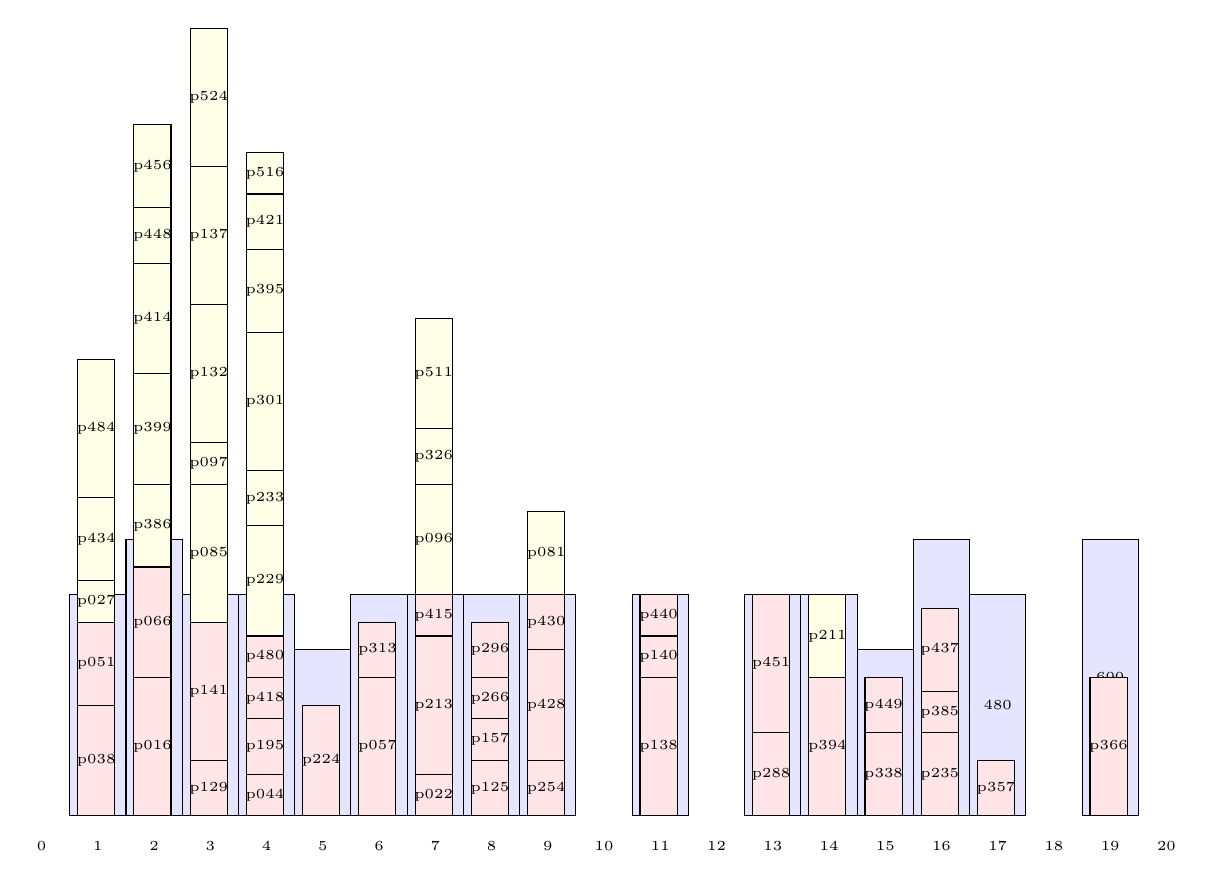
\begin{tikzpicture}[xscale=1.000000,yscale=1.000000]
\node[below] () at (0.357143,-0.2) {\tiny 0};
\node[below] () at (1.071429,-0.2) {\tiny 1};
\node[below] () at (1.785714,-0.2) {\tiny 2};
\node[below] () at (2.500000,-0.2) {\tiny 3};
\node[below] () at (3.214286,-0.2) {\tiny 4};
\node[below] () at (3.928571,-0.2) {\tiny 5};
\node[below] () at (4.642857,-0.2) {\tiny 6};
\node[below] () at (5.357143,-0.2) {\tiny 7};
\node[below] () at (6.071429,-0.2) {\tiny 8};
\node[below] () at (6.785714,-0.2) {\tiny 9};
\node[below] () at (7.500000,-0.2) {\tiny 10};
\node[below] () at (8.214286,-0.2) {\tiny 11};
\node[below] () at (8.928571,-0.2) {\tiny 12};
\node[below] () at (9.642857,-0.2) {\tiny 13};
\node[below] () at (10.357143,-0.2) {\tiny 14};
\node[below] () at (11.071429,-0.2) {\tiny 15};
\node[below] () at (11.785714,-0.2) {\tiny 16};
\node[below] () at (12.500000,-0.2) {\tiny 17};
\node[below] () at (13.214286,-0.2) {\tiny 18};
\node[below] () at (13.928571,-0.2) {\tiny 19};
\node[below] () at (14.642857,-0.2) {\tiny 20};
\draw[draw=black,fill=blue!10] (0.714286,0.000000) rectangle node {\tiny 480} (1.428571,2.807018);
\draw[fill=red!10] (0.814286,0.000000) rectangle node {\tiny p038} (1.285714,1.403509);
\draw[fill=red!10] (0.814286,1.403509) rectangle node {\tiny p051} (1.285714,2.456140);
\draw[fill=yellow!10] (0.814286,2.456140) rectangle node {\tiny p027} (1.285714,2.982456);
\draw[fill=yellow!10] (0.814286,2.982456) rectangle node {\tiny p434} (1.285714,4.035088);
\draw[fill=yellow!10] (0.814286,4.035088) rectangle node {\tiny p484} (1.285714,5.789474);
\draw[draw=black,fill=blue!10] (1.428571,0.000000) rectangle node {\tiny 600} (2.142857,3.508772);
\draw[fill=red!10] (1.528571,0.000000) rectangle node {\tiny p016} (2.000000,1.754386);
\draw[fill=red!10] (1.528571,1.754386) rectangle node {\tiny p066} (2.000000,3.157895);
\draw[fill=yellow!10] (1.528571,3.157895) rectangle node {\tiny p386} (2.000000,4.210526);
\draw[fill=yellow!10] (1.528571,4.210526) rectangle node {\tiny p399} (2.000000,5.614035);
\draw[fill=yellow!10] (1.528571,5.614035) rectangle node {\tiny p414} (2.000000,7.017544);
\draw[fill=yellow!10] (1.528571,7.017544) rectangle node {\tiny p448} (2.000000,7.719298);
\draw[fill=yellow!10] (1.528571,7.719298) rectangle node {\tiny p456} (2.000000,8.771930);
\draw[draw=black,fill=blue!10] (2.142857,0.000000) rectangle node {\tiny 480} (2.857143,2.807018);
\draw[fill=red!10] (2.242857,0.000000) rectangle node {\tiny p129} (2.714286,0.701754);
\draw[fill=red!10] (2.242857,0.701754) rectangle node {\tiny p141} (2.714286,2.456140);
\draw[fill=yellow!10] (2.242857,2.456140) rectangle node {\tiny p085} (2.714286,4.210526);
\draw[fill=yellow!10] (2.242857,4.210526) rectangle node {\tiny p097} (2.714286,4.736842);
\draw[fill=yellow!10] (2.242857,4.736842) rectangle node {\tiny p132} (2.714286,6.491228);
\draw[fill=yellow!10] (2.242857,6.491228) rectangle node {\tiny p137} (2.714286,8.245614);
\draw[fill=yellow!10] (2.242857,8.245614) rectangle node {\tiny p524} (2.714286,10.000000);
\draw[draw=black,fill=blue!10] (2.857143,0.000000) rectangle node {\tiny 480} (3.571429,2.807018);
\draw[fill=red!10] (2.957143,0.000000) rectangle node {\tiny p044} (3.428571,0.526316);
\draw[fill=red!10] (2.957143,0.526316) rectangle node {\tiny p195} (3.428571,1.228070);
\draw[fill=red!10] (2.957143,1.228070) rectangle node {\tiny p418} (3.428571,1.754386);
\draw[fill=red!10] (2.957143,1.754386) rectangle node {\tiny p480} (3.428571,2.280702);
\draw[fill=yellow!10] (2.957143,2.280702) rectangle node {\tiny p229} (3.428571,3.684211);
\draw[fill=yellow!10] (2.957143,3.684211) rectangle node {\tiny p233} (3.428571,4.385965);
\draw[fill=yellow!10] (2.957143,4.385965) rectangle node {\tiny p301} (3.428571,6.140351);
\draw[fill=yellow!10] (2.957143,6.140351) rectangle node {\tiny p395} (3.428571,7.192982);
\draw[fill=yellow!10] (2.957143,7.192982) rectangle node {\tiny p421} (3.428571,7.894737);
\draw[fill=yellow!10] (2.957143,7.894737) rectangle node {\tiny p516} (3.428571,8.421053);
\draw[draw=black,fill=blue!10] (3.571429,0.000000) rectangle node {\tiny 360} (4.285714,2.105263);
\draw[fill=red!10] (3.671429,0.000000) rectangle node {\tiny p224} (4.142857,1.403509);
\draw[draw=black,fill=blue!10] (4.285714,0.000000) rectangle node {\tiny 480} (5.000000,2.807018);
\draw[fill=red!10] (4.385714,0.000000) rectangle node {\tiny p057} (4.857143,1.754386);
\draw[fill=red!10] (4.385714,1.754386) rectangle node {\tiny p313} (4.857143,2.456140);
\draw[draw=black,fill=blue!10] (5.000000,0.000000) rectangle node {\tiny 480} (5.714286,2.807018);
\draw[fill=red!10] (5.100000,0.000000) rectangle node {\tiny p022} (5.571429,0.526316);
\draw[fill=red!10] (5.100000,0.526316) rectangle node {\tiny p213} (5.571429,2.280702);
\draw[fill=red!10] (5.100000,2.280702) rectangle node {\tiny p415} (5.571429,2.807018);
\draw[fill=yellow!10] (5.100000,2.807018) rectangle node {\tiny p096} (5.571429,4.210526);
\draw[fill=yellow!10] (5.100000,4.210526) rectangle node {\tiny p326} (5.571429,4.912281);
\draw[fill=yellow!10] (5.100000,4.912281) rectangle node {\tiny p511} (5.571429,6.315789);
\draw[draw=black,fill=blue!10] (5.714286,0.000000) rectangle node {\tiny 480} (6.428571,2.807018);
\draw[fill=red!10] (5.814286,0.000000) rectangle node {\tiny p125} (6.285714,0.701754);
\draw[fill=red!10] (5.814286,0.701754) rectangle node {\tiny p157} (6.285714,1.228070);
\draw[fill=red!10] (5.814286,1.228070) rectangle node {\tiny p266} (6.285714,1.754386);
\draw[fill=red!10] (5.814286,1.754386) rectangle node {\tiny p296} (6.285714,2.456140);
\draw[draw=black,fill=blue!10] (6.428571,0.000000) rectangle node {\tiny 480} (7.142857,2.807018);
\draw[fill=red!10] (6.528571,0.000000) rectangle node {\tiny p254} (7.000000,0.701754);
\draw[fill=red!10] (6.528571,0.701754) rectangle node {\tiny p428} (7.000000,2.105263);
\draw[fill=red!10] (6.528571,2.105263) rectangle node {\tiny p430} (7.000000,2.807018);
\draw[fill=yellow!10] (6.528571,2.807018) rectangle node {\tiny p081} (7.000000,3.859649);
\draw[draw=black,fill=blue!10] (7.857143,0.000000) rectangle node {\tiny 480} (8.571429,2.807018);
\draw[fill=red!10] (7.957143,0.000000) rectangle node {\tiny p138} (8.428571,1.754386);
\draw[fill=red!10] (7.957143,1.754386) rectangle node {\tiny p140} (8.428571,2.280702);
\draw[fill=red!10] (7.957143,2.280702) rectangle node {\tiny p440} (8.428571,2.807018);
\draw[draw=black,fill=blue!10] (9.285714,0.000000) rectangle node {\tiny 480} (10.000000,2.807018);
\draw[fill=red!10] (9.385714,0.000000) rectangle node {\tiny p288} (9.857143,1.052632);
\draw[fill=red!10] (9.385714,1.052632) rectangle node {\tiny p451} (9.857143,2.807018);
\draw[draw=black,fill=blue!10] (10.000000,0.000000) rectangle node {\tiny 480} (10.714286,2.807018);
\draw[fill=red!10] (10.100000,0.000000) rectangle node {\tiny p394} (10.571429,1.754386);
\draw[fill=yellow!10] (10.100000,1.754386) rectangle node {\tiny p211} (10.571429,2.807018);
\draw[draw=black,fill=blue!10] (10.714286,0.000000) rectangle node {\tiny 360} (11.428571,2.105263);
\draw[fill=red!10] (10.814286,0.000000) rectangle node {\tiny p338} (11.285714,1.052632);
\draw[fill=red!10] (10.814286,1.052632) rectangle node {\tiny p449} (11.285714,1.754386);
\draw[draw=black,fill=blue!10] (11.428571,0.000000) rectangle node {\tiny 600} (12.142857,3.508772);
\draw[fill=red!10] (11.528571,0.000000) rectangle node {\tiny p235} (12.000000,1.052632);
\draw[fill=red!10] (11.528571,1.052632) rectangle node {\tiny p385} (12.000000,1.578947);
\draw[fill=red!10] (11.528571,1.578947) rectangle node {\tiny p437} (12.000000,2.631579);
\draw[draw=black,fill=blue!10] (12.142857,0.000000) rectangle node {\tiny 480} (12.857143,2.807018);
\draw[fill=red!10] (12.242857,0.000000) rectangle node {\tiny p357} (12.714286,0.701754);
\draw[draw=black,fill=blue!10] (13.571429,0.000000) rectangle node {\tiny 600} (14.285714,3.508772);
\draw[fill=red!10] (13.671429,0.000000) rectangle node {\tiny p366} (14.142857,1.754386);
\end{tikzpicture}

}
 \begin{textblock}{4}(11,5)
  Patients shown on release day
 \end{textblock}
 \begin{textblock}{4}(11,8)
  Not much capacity left for optional patients
 \end{textblock}
\end{frame}

\begin{frame}
\frametitle{Results of Analysis}
\begin{itemize}
\item Finding which patients to admit will be the most important choice. 
\item To utilise the full surgeon capacity, we will have to delay admission of some patients to use the available time  slots.
\item We do  not have to consider the detailed theatre assignment when making the initial admission selection.
\item When admitting a patient, we must have a bed for their full stay available. Estimating full capacity is tough.
\item We can initially ignore the nurse workload/skill limits, and age mix constraints as well.
\end{itemize}
\end{frame}

\subsection{Decomposition}

\begin{frame}[fragile]
\frametitle{The Resulting Decomposition}
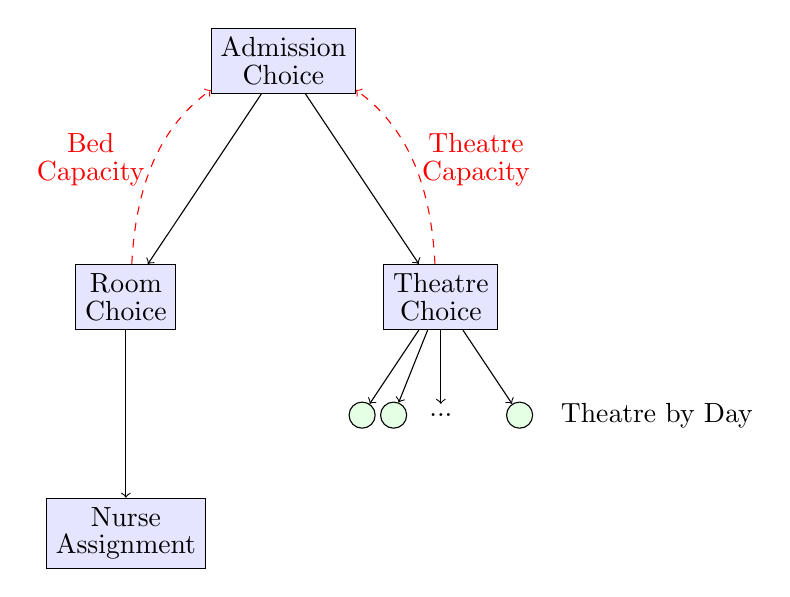
\begin{tikzpicture}[xscale=2,yscale=3]
\node[fill=blue!10,draw=black] (admission) at (2,3) {\shortstack{Admission\\Choice}};
\node[fill=blue!10,draw=black] (theatre) at (3,2) {\shortstack{Theatre\\Choice}};
\node[circle,fill=green!10,draw=black] (d1) at (2.5,1.5) {};
\node[circle,fill=green!10,draw=black] (d2) at (2.7,1.5) {};
\node[draw=none] (dj) at (3,1.5) {...};
\node[circle,fill=green!10,draw=black] (dn) at (3.5,1.5) {};
\node[right,draw=none] () at (3.7,1.5) {Theatre by Day};
\node[fill=blue!10,draw=black] (room) at (1,2) {\shortstack{Room\\Choice}};
\node[fill=blue!10,draw=black] (nurse) at (1,1) {\shortstack{Nurse\\Assignment}};
\draw[->] (admission) -- (theatre);
\draw[->] (admission) -- (room);
\draw[->] (room) -- (nurse);
\draw[->] (theatre) -- (d1);
\draw[->] (theatre) -- (d2);
\draw[->] (theatre) -- (dj);
\draw[->] (theatre) -- (dn);

\draw[red,dashed,->] (theatre) to[bend right] node[right]{\shortstack{Theatre\\Capacity}} (admission);
\draw[red,dashed,->] (room) to[bend left] node[left] {\shortstack{Bed\\Capacity}} (admission);

\end{tikzpicture}

\end{frame}

\begin{frame}
\frametitle{Stages}
\begin{description}
\item[Admission] decide which patients to admit when
\item[Room] assign a room/bed to each selected
\item[Theatre] assign a theatre to each patient
\item[Nurse Assignment] assign a nurse to each (non-empty) room
\end{description}
\end{frame}



\subsection{Results}

\begin{frame}
\frametitle{Sample solution test10, total surgeon utilisation}
\scalebox{0.7}{
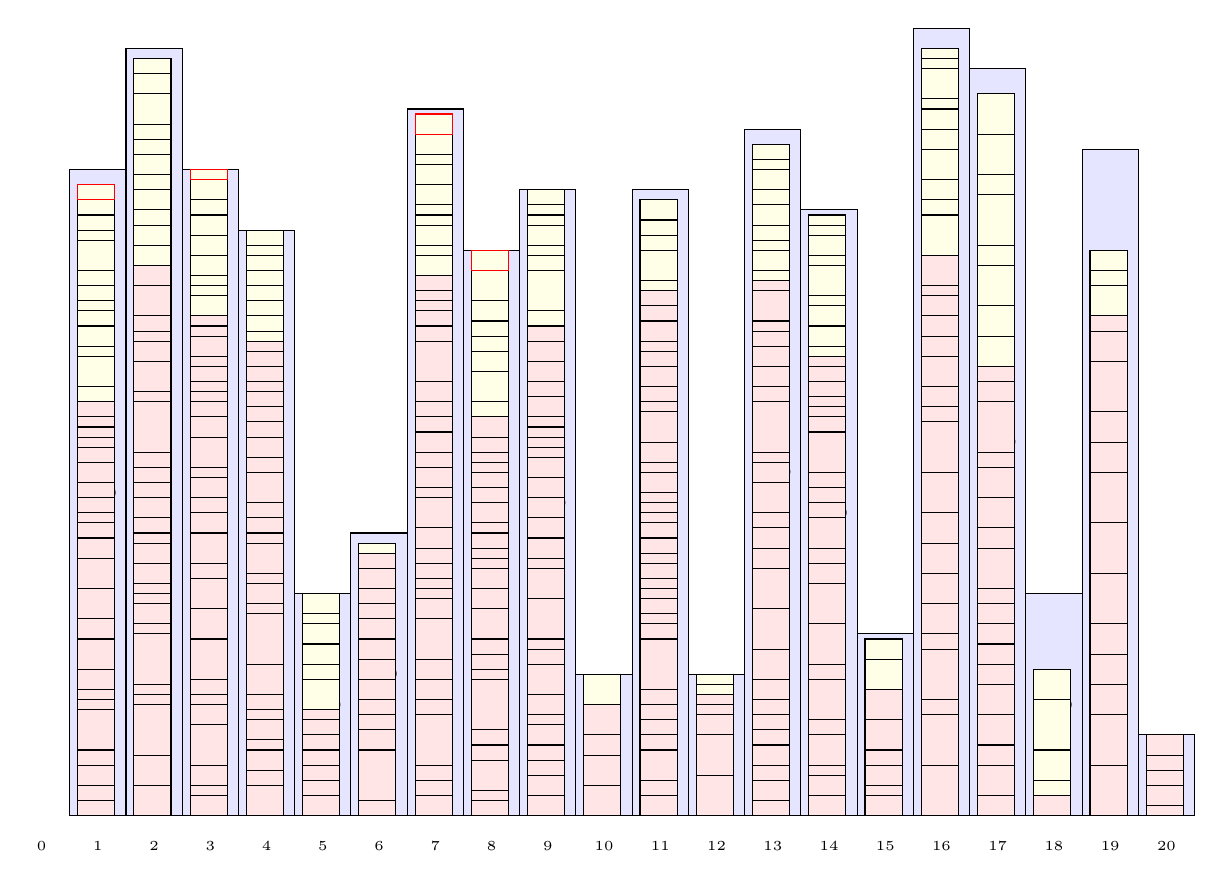
\begin{tikzpicture}[xscale=1.000000,yscale=1.000000]
\node[below] () at (0.357143,-0.2) {\tiny 0};
\node[below] () at (1.071429,-0.2) {\tiny 1};
\node[below] () at (1.785714,-0.2) {\tiny 2};
\node[below] () at (2.500000,-0.2) {\tiny 3};
\node[below] () at (3.214286,-0.2) {\tiny 4};
\node[below] () at (3.928571,-0.2) {\tiny 5};
\node[below] () at (4.642857,-0.2) {\tiny 6};
\node[below] () at (5.357143,-0.2) {\tiny 7};
\node[below] () at (6.071429,-0.2) {\tiny 8};
\node[below] () at (6.785714,-0.2) {\tiny 9};
\node[below] () at (7.500000,-0.2) {\tiny 10};
\node[below] () at (8.214286,-0.2) {\tiny 11};
\node[below] () at (8.928571,-0.2) {\tiny 12};
\node[below] () at (9.642857,-0.2) {\tiny 13};
\node[below] () at (10.357143,-0.2) {\tiny 14};
\node[below] () at (11.071429,-0.2) {\tiny 15};
\node[below] () at (11.785714,-0.2) {\tiny 16};
\node[below] () at (12.500000,-0.2) {\tiny 17};
\node[below] () at (13.214286,-0.2) {\tiny 18};
\node[below] () at (13.928571,-0.2) {\tiny 19};
\node[below] () at (14.642857,-0.2) {\tiny 20};
\draw[draw=black,fill=blue!10] (0.714286,0.000000) rectangle node {\tiny 3840} (1.428571,8.205128);
\draw[fill=red!10] (0.814286,0.000000) rectangle node {\tiny } (1.285714,0.192308);
\draw[fill=red!10] (0.814286,0.192308) rectangle node {\tiny } (1.285714,0.384615);
\draw[fill=red!10] (0.814286,0.384615) rectangle node {\tiny } (1.285714,0.641026);
\draw[fill=red!10] (0.814286,0.641026) rectangle node {\tiny } (1.285714,0.833333);
\draw[fill=red!10] (0.814286,0.833333) rectangle node {\tiny } (1.285714,1.346154);
\draw[fill=red!10] (0.814286,1.346154) rectangle node {\tiny } (1.285714,1.474359);
\draw[fill=red!10] (0.814286,1.474359) rectangle node {\tiny } (1.285714,1.602564);
\draw[fill=red!10] (0.814286,1.602564) rectangle node {\tiny } (1.285714,1.858974);
\draw[fill=red!10] (0.814286,1.858974) rectangle node {\tiny } (1.285714,2.243590);
\draw[fill=red!10] (0.814286,2.243590) rectangle node {\tiny } (1.285714,2.500000);
\draw[fill=red!10] (0.814286,2.500000) rectangle node {\tiny } (1.285714,2.884615);
\draw[fill=red!10] (0.814286,2.884615) rectangle node {\tiny } (1.285714,3.269231);
\draw[fill=red!10] (0.814286,3.269231) rectangle node {\tiny } (1.285714,3.525641);
\draw[fill=red!10] (0.814286,3.525641) rectangle node {\tiny } (1.285714,3.717949);
\draw[fill=red!10] (0.814286,3.717949) rectangle node {\tiny } (1.285714,3.846154);
\draw[fill=red!10] (0.814286,3.846154) rectangle node {\tiny } (1.285714,4.038462);
\draw[fill=red!10] (0.814286,4.038462) rectangle node {\tiny } (1.285714,4.230769);
\draw[fill=red!10] (0.814286,4.230769) rectangle node {\tiny } (1.285714,4.487179);
\draw[fill=red!10] (0.814286,4.487179) rectangle node {\tiny } (1.285714,4.679487);
\draw[fill=red!10] (0.814286,4.679487) rectangle node {\tiny } (1.285714,4.807692);
\draw[fill=red!10] (0.814286,4.807692) rectangle node {\tiny } (1.285714,4.935897);
\draw[fill=red!10] (0.814286,4.935897) rectangle node {\tiny } (1.285714,5.064103);
\draw[fill=red!10] (0.814286,5.064103) rectangle node {\tiny } (1.285714,5.256410);
\draw[fill=yellow!10] (0.814286,5.256410) rectangle node {\tiny } (1.285714,5.448718);
\draw[fill=yellow!10] (0.814286,5.448718) rectangle node {\tiny } (1.285714,5.833333);
\draw[fill=yellow!10] (0.814286,5.833333) rectangle node {\tiny } (1.285714,5.961538);
\draw[fill=yellow!10] (0.814286,5.961538) rectangle node {\tiny } (1.285714,6.217949);
\draw[fill=yellow!10] (0.814286,6.217949) rectangle node {\tiny } (1.285714,6.410256);
\draw[fill=yellow!10] (0.814286,6.410256) rectangle node {\tiny } (1.285714,6.538462);
\draw[fill=yellow!10] (0.814286,6.538462) rectangle node {\tiny } (1.285714,6.730769);
\draw[fill=yellow!10] (0.814286,6.730769) rectangle node {\tiny } (1.285714,6.923077);
\draw[fill=yellow!10] (0.814286,6.923077) rectangle node {\tiny } (1.285714,7.307692);
\draw[fill=yellow!10] (0.814286,7.307692) rectangle node {\tiny } (1.285714,7.435897);
\draw[fill=yellow!10] (0.814286,7.435897) rectangle node {\tiny } (1.285714,7.628205);
\draw[fill=yellow!10] (0.814286,7.628205) rectangle node {\tiny } (1.285714,7.820513);
\draw[draw=red,fill=yellow!10] (0.814286,7.820513) rectangle node {\tiny } (1.285714,8.012821);
\draw[draw=black,fill=blue!10] (1.428571,0.000000) rectangle node {\tiny 4560} (2.142857,9.743590);
\draw[fill=red!10] (1.528571,0.000000) rectangle node {\tiny } (2.000000,0.384615);
\draw[fill=red!10] (1.528571,0.384615) rectangle node {\tiny } (2.000000,0.769231);
\draw[fill=red!10] (1.528571,0.769231) rectangle node {\tiny } (2.000000,1.410256);
\draw[fill=red!10] (1.528571,1.410256) rectangle node {\tiny } (2.000000,1.538462);
\draw[fill=red!10] (1.528571,1.538462) rectangle node {\tiny } (2.000000,1.666667);
\draw[fill=red!10] (1.528571,1.666667) rectangle node {\tiny } (2.000000,2.307692);
\draw[fill=red!10] (1.528571,2.307692) rectangle node {\tiny } (2.000000,2.435897);
\draw[fill=red!10] (1.528571,2.435897) rectangle node {\tiny } (2.000000,2.692308);
\draw[fill=red!10] (1.528571,2.692308) rectangle node {\tiny } (2.000000,2.820513);
\draw[fill=red!10] (1.528571,2.820513) rectangle node {\tiny } (2.000000,2.948718);
\draw[fill=red!10] (1.528571,2.948718) rectangle node {\tiny } (2.000000,3.205128);
\draw[fill=red!10] (1.528571,3.205128) rectangle node {\tiny } (2.000000,3.461538);
\draw[fill=red!10] (1.528571,3.461538) rectangle node {\tiny } (2.000000,3.589744);
\draw[fill=red!10] (1.528571,3.589744) rectangle node {\tiny } (2.000000,3.782051);
\draw[fill=red!10] (1.528571,3.782051) rectangle node {\tiny } (2.000000,4.038462);
\draw[fill=red!10] (1.528571,4.038462) rectangle node {\tiny } (2.000000,4.230769);
\draw[fill=red!10] (1.528571,4.230769) rectangle node {\tiny } (2.000000,4.423077);
\draw[fill=red!10] (1.528571,4.423077) rectangle node {\tiny } (2.000000,4.615385);
\draw[fill=red!10] (1.528571,4.615385) rectangle node {\tiny } (2.000000,5.256410);
\draw[fill=red!10] (1.528571,5.256410) rectangle node {\tiny } (2.000000,5.384615);
\draw[fill=red!10] (1.528571,5.384615) rectangle node {\tiny } (2.000000,5.769231);
\draw[fill=red!10] (1.528571,5.769231) rectangle node {\tiny } (2.000000,6.025641);
\draw[fill=red!10] (1.528571,6.025641) rectangle node {\tiny } (2.000000,6.153846);
\draw[fill=red!10] (1.528571,6.153846) rectangle node {\tiny } (2.000000,6.346154);
\draw[fill=red!10] (1.528571,6.346154) rectangle node {\tiny } (2.000000,6.730769);
\draw[fill=red!10] (1.528571,6.730769) rectangle node {\tiny } (2.000000,6.987179);
\draw[fill=yellow!10] (1.528571,6.987179) rectangle node {\tiny } (2.000000,7.243590);
\draw[fill=yellow!10] (1.528571,7.243590) rectangle node {\tiny } (2.000000,7.500000);
\draw[fill=yellow!10] (1.528571,7.500000) rectangle node {\tiny } (2.000000,7.692308);
\draw[fill=yellow!10] (1.528571,7.692308) rectangle node {\tiny } (2.000000,7.948718);
\draw[fill=yellow!10] (1.528571,7.948718) rectangle node {\tiny } (2.000000,8.141026);
\draw[fill=yellow!10] (1.528571,8.141026) rectangle node {\tiny } (2.000000,8.397436);
\draw[fill=yellow!10] (1.528571,8.397436) rectangle node {\tiny } (2.000000,8.589744);
\draw[fill=yellow!10] (1.528571,8.589744) rectangle node {\tiny } (2.000000,8.782051);
\draw[fill=yellow!10] (1.528571,8.782051) rectangle node {\tiny } (2.000000,9.166667);
\draw[fill=yellow!10] (1.528571,9.166667) rectangle node {\tiny } (2.000000,9.423077);
\draw[fill=yellow!10] (1.528571,9.423077) rectangle node {\tiny } (2.000000,9.615385);
\draw[draw=black,fill=blue!10] (2.142857,0.000000) rectangle node {\tiny 3840} (2.857143,8.205128);
\draw[fill=red!10] (2.242857,0.000000) rectangle node {\tiny } (2.714286,0.256410);
\draw[fill=red!10] (2.242857,0.256410) rectangle node {\tiny } (2.714286,0.384615);
\draw[fill=red!10] (2.242857,0.384615) rectangle node {\tiny } (2.714286,0.641026);
\draw[fill=red!10] (2.242857,0.641026) rectangle node {\tiny } (2.714286,1.153846);
\draw[fill=red!10] (2.242857,1.153846) rectangle node {\tiny } (2.714286,1.410256);
\draw[fill=red!10] (2.242857,1.410256) rectangle node {\tiny } (2.714286,1.538462);
\draw[fill=red!10] (2.242857,1.538462) rectangle node {\tiny } (2.714286,1.730769);
\draw[fill=red!10] (2.242857,1.730769) rectangle node {\tiny } (2.714286,2.243590);
\draw[fill=red!10] (2.242857,2.243590) rectangle node {\tiny } (2.714286,2.628205);
\draw[fill=red!10] (2.242857,2.628205) rectangle node {\tiny } (2.714286,3.012821);
\draw[fill=red!10] (2.242857,3.012821) rectangle node {\tiny } (2.714286,3.205128);
\draw[fill=red!10] (2.242857,3.205128) rectangle node {\tiny } (2.714286,3.589744);
\draw[fill=red!10] (2.242857,3.589744) rectangle node {\tiny } (2.714286,3.846154);
\draw[fill=red!10] (2.242857,3.846154) rectangle node {\tiny } (2.714286,4.038462);
\draw[fill=red!10] (2.242857,4.038462) rectangle node {\tiny } (2.714286,4.294872);
\draw[fill=red!10] (2.242857,4.294872) rectangle node {\tiny } (2.714286,4.423077);
\draw[fill=red!10] (2.242857,4.423077) rectangle node {\tiny } (2.714286,4.807692);
\draw[fill=red!10] (2.242857,4.807692) rectangle node {\tiny } (2.714286,5.064103);
\draw[fill=red!10] (2.242857,5.064103) rectangle node {\tiny } (2.714286,5.256410);
\draw[fill=red!10] (2.242857,5.256410) rectangle node {\tiny } (2.714286,5.384615);
\draw[fill=red!10] (2.242857,5.384615) rectangle node {\tiny } (2.714286,5.512821);
\draw[fill=red!10] (2.242857,5.512821) rectangle node {\tiny } (2.714286,5.705128);
\draw[fill=red!10] (2.242857,5.705128) rectangle node {\tiny } (2.714286,5.833333);
\draw[fill=red!10] (2.242857,5.833333) rectangle node {\tiny } (2.714286,6.089744);
\draw[fill=red!10] (2.242857,6.089744) rectangle node {\tiny } (2.714286,6.217949);
\draw[fill=red!10] (2.242857,6.217949) rectangle node {\tiny } (2.714286,6.346154);
\draw[fill=yellow!10] (2.242857,6.346154) rectangle node {\tiny } (2.714286,6.602564);
\draw[fill=yellow!10] (2.242857,6.602564) rectangle node {\tiny } (2.714286,6.730769);
\draw[fill=yellow!10] (2.242857,6.730769) rectangle node {\tiny } (2.714286,6.858974);
\draw[fill=yellow!10] (2.242857,6.858974) rectangle node {\tiny } (2.714286,7.115385);
\draw[fill=yellow!10] (2.242857,7.115385) rectangle node {\tiny } (2.714286,7.371795);
\draw[fill=yellow!10] (2.242857,7.371795) rectangle node {\tiny } (2.714286,7.628205);
\draw[fill=yellow!10] (2.242857,7.628205) rectangle node {\tiny } (2.714286,7.820513);
\draw[fill=yellow!10] (2.242857,7.820513) rectangle node {\tiny } (2.714286,8.076923);
\draw[draw=red,fill=yellow!10] (2.242857,8.076923) rectangle node {\tiny } (2.714286,8.205128);
\draw[draw=black,fill=blue!10] (2.857143,0.000000) rectangle node {\tiny 3480} (3.571429,7.435897);
\draw[fill=red!10] (2.957143,0.000000) rectangle node {\tiny } (3.428571,0.384615);
\draw[fill=red!10] (2.957143,0.384615) rectangle node {\tiny } (3.428571,0.576923);
\draw[fill=red!10] (2.957143,0.576923) rectangle node {\tiny } (3.428571,0.833333);
\draw[fill=red!10] (2.957143,0.833333) rectangle node {\tiny } (3.428571,0.961538);
\draw[fill=red!10] (2.957143,0.961538) rectangle node {\tiny } (3.428571,1.217949);
\draw[fill=red!10] (2.957143,1.217949) rectangle node {\tiny } (3.428571,1.346154);
\draw[fill=red!10] (2.957143,1.346154) rectangle node {\tiny } (3.428571,1.538462);
\draw[fill=red!10] (2.957143,1.538462) rectangle node {\tiny } (3.428571,1.923077);
\draw[fill=red!10] (2.957143,1.923077) rectangle node {\tiny } (3.428571,2.564103);
\draw[fill=red!10] (2.957143,2.564103) rectangle node {\tiny } (3.428571,2.692308);
\draw[fill=red!10] (2.957143,2.692308) rectangle node {\tiny } (3.428571,2.948718);
\draw[fill=red!10] (2.957143,2.948718) rectangle node {\tiny } (3.428571,3.076923);
\draw[fill=red!10] (2.957143,3.076923) rectangle node {\tiny } (3.428571,3.461538);
\draw[fill=red!10] (2.957143,3.461538) rectangle node {\tiny } (3.428571,3.589744);
\draw[fill=red!10] (2.957143,3.589744) rectangle node {\tiny } (3.428571,3.782051);
\draw[fill=red!10] (2.957143,3.782051) rectangle node {\tiny } (3.428571,3.974359);
\draw[fill=red!10] (2.957143,3.974359) rectangle node {\tiny } (3.428571,4.358974);
\draw[fill=red!10] (2.957143,4.358974) rectangle node {\tiny } (3.428571,4.551282);
\draw[fill=red!10] (2.957143,4.551282) rectangle node {\tiny } (3.428571,4.807692);
\draw[fill=red!10] (2.957143,4.807692) rectangle node {\tiny } (3.428571,5.000000);
\draw[fill=red!10] (2.957143,5.000000) rectangle node {\tiny } (3.428571,5.192308);
\draw[fill=red!10] (2.957143,5.192308) rectangle node {\tiny } (3.428571,5.384615);
\draw[fill=red!10] (2.957143,5.384615) rectangle node {\tiny } (3.428571,5.512821);
\draw[fill=red!10] (2.957143,5.512821) rectangle node {\tiny } (3.428571,5.705128);
\draw[fill=red!10] (2.957143,5.705128) rectangle node {\tiny } (3.428571,5.897436);
\draw[fill=red!10] (2.957143,5.897436) rectangle node {\tiny } (3.428571,6.025641);
\draw[fill=yellow!10] (2.957143,6.025641) rectangle node {\tiny } (3.428571,6.153846);
\draw[fill=yellow!10] (2.957143,6.153846) rectangle node {\tiny } (3.428571,6.346154);
\draw[fill=yellow!10] (2.957143,6.346154) rectangle node {\tiny } (3.428571,6.538462);
\draw[fill=yellow!10] (2.957143,6.538462) rectangle node {\tiny } (3.428571,6.730769);
\draw[fill=yellow!10] (2.957143,6.730769) rectangle node {\tiny } (3.428571,6.923077);
\draw[fill=yellow!10] (2.957143,6.923077) rectangle node {\tiny } (3.428571,7.115385);
\draw[fill=yellow!10] (2.957143,7.115385) rectangle node {\tiny } (3.428571,7.243590);
\draw[fill=yellow!10] (2.957143,7.243590) rectangle node {\tiny } (3.428571,7.435897);
\draw[draw=black,fill=blue!10] (3.571429,0.000000) rectangle node {\tiny 1320} (4.285714,2.820513);
\draw[fill=red!10] (3.671429,0.000000) rectangle node {\tiny } (4.142857,0.256410);
\draw[fill=red!10] (3.671429,0.256410) rectangle node {\tiny } (4.142857,0.448718);
\draw[fill=red!10] (3.671429,0.448718) rectangle node {\tiny } (4.142857,0.641026);
\draw[fill=red!10] (3.671429,0.641026) rectangle node {\tiny } (4.142857,0.833333);
\draw[fill=red!10] (3.671429,0.833333) rectangle node {\tiny } (4.142857,1.025641);
\draw[fill=red!10] (3.671429,1.025641) rectangle node {\tiny } (4.142857,1.217949);
\draw[fill=red!10] (3.671429,1.217949) rectangle node {\tiny } (4.142857,1.346154);
\draw[fill=yellow!10] (3.671429,1.346154) rectangle node {\tiny } (4.142857,1.730769);
\draw[fill=yellow!10] (3.671429,1.730769) rectangle node {\tiny } (4.142857,1.923077);
\draw[fill=yellow!10] (3.671429,1.923077) rectangle node {\tiny } (4.142857,2.179487);
\draw[fill=yellow!10] (3.671429,2.179487) rectangle node {\tiny } (4.142857,2.435897);
\draw[fill=yellow!10] (3.671429,2.435897) rectangle node {\tiny } (4.142857,2.564103);
\draw[fill=yellow!10] (3.671429,2.564103) rectangle node {\tiny } (4.142857,2.820513);
\draw[draw=black,fill=blue!10] (4.285714,0.000000) rectangle node {\tiny 1680} (5.000000,3.589744);
\draw[fill=red!10] (4.385714,0.000000) rectangle node {\tiny } (4.857143,0.192308);
\draw[fill=red!10] (4.385714,0.192308) rectangle node {\tiny } (4.857143,0.833333);
\draw[fill=red!10] (4.385714,0.833333) rectangle node {\tiny } (4.857143,1.089744);
\draw[fill=red!10] (4.385714,1.089744) rectangle node {\tiny } (4.857143,1.282051);
\draw[fill=red!10] (4.385714,1.282051) rectangle node {\tiny } (4.857143,1.474359);
\draw[fill=red!10] (4.385714,1.474359) rectangle node {\tiny } (4.857143,1.730769);
\draw[fill=red!10] (4.385714,1.730769) rectangle node {\tiny } (4.857143,1.987179);
\draw[fill=red!10] (4.385714,1.987179) rectangle node {\tiny } (4.857143,2.243590);
\draw[fill=red!10] (4.385714,2.243590) rectangle node {\tiny } (4.857143,2.500000);
\draw[fill=red!10] (4.385714,2.500000) rectangle node {\tiny } (4.857143,2.692308);
\draw[fill=red!10] (4.385714,2.692308) rectangle node {\tiny } (4.857143,2.884615);
\draw[fill=red!10] (4.385714,2.884615) rectangle node {\tiny } (4.857143,3.141026);
\draw[fill=red!10] (4.385714,3.141026) rectangle node {\tiny } (4.857143,3.333333);
\draw[fill=yellow!10] (4.385714,3.333333) rectangle node {\tiny } (4.857143,3.461538);
\draw[draw=black,fill=blue!10] (5.000000,0.000000) rectangle node {\tiny 4200} (5.714286,8.974359);
\draw[fill=red!10] (5.100000,0.000000) rectangle node {\tiny } (5.571429,0.256410);
\draw[fill=red!10] (5.100000,0.256410) rectangle node {\tiny } (5.571429,0.448718);
\draw[fill=red!10] (5.100000,0.448718) rectangle node {\tiny } (5.571429,0.641026);
\draw[fill=red!10] (5.100000,0.641026) rectangle node {\tiny } (5.571429,1.282051);
\draw[fill=red!10] (5.100000,1.282051) rectangle node {\tiny } (5.571429,1.474359);
\draw[fill=red!10] (5.100000,1.474359) rectangle node {\tiny } (5.571429,1.730769);
\draw[fill=red!10] (5.100000,1.730769) rectangle node {\tiny } (5.571429,1.987179);
\draw[fill=red!10] (5.100000,1.987179) rectangle node {\tiny } (5.571429,2.500000);
\draw[fill=red!10] (5.100000,2.500000) rectangle node {\tiny } (5.571429,2.756410);
\draw[fill=red!10] (5.100000,2.756410) rectangle node {\tiny } (5.571429,2.884615);
\draw[fill=red!10] (5.100000,2.884615) rectangle node {\tiny } (5.571429,3.012821);
\draw[fill=red!10] (5.100000,3.012821) rectangle node {\tiny } (5.571429,3.205128);
\draw[fill=red!10] (5.100000,3.205128) rectangle node {\tiny } (5.571429,3.397436);
\draw[fill=red!10] (5.100000,3.397436) rectangle node {\tiny } (5.571429,3.653846);
\draw[fill=red!10] (5.100000,3.653846) rectangle node {\tiny } (5.571429,4.038462);
\draw[fill=red!10] (5.100000,4.038462) rectangle node {\tiny } (5.571429,4.166667);
\draw[fill=red!10] (5.100000,4.166667) rectangle node {\tiny } (5.571429,4.423077);
\draw[fill=red!10] (5.100000,4.423077) rectangle node {\tiny } (5.571429,4.615385);
\draw[fill=red!10] (5.100000,4.615385) rectangle node {\tiny } (5.571429,4.871795);
\draw[fill=red!10] (5.100000,4.871795) rectangle node {\tiny } (5.571429,5.064103);
\draw[fill=red!10] (5.100000,5.064103) rectangle node {\tiny } (5.571429,5.256410);
\draw[fill=red!10] (5.100000,5.256410) rectangle node {\tiny } (5.571429,5.512821);
\draw[fill=red!10] (5.100000,5.512821) rectangle node {\tiny } (5.571429,6.025641);
\draw[fill=red!10] (5.100000,6.025641) rectangle node {\tiny } (5.571429,6.217949);
\draw[fill=red!10] (5.100000,6.217949) rectangle node {\tiny } (5.571429,6.410256);
\draw[fill=red!10] (5.100000,6.410256) rectangle node {\tiny } (5.571429,6.538462);
\draw[fill=red!10] (5.100000,6.538462) rectangle node {\tiny } (5.571429,6.666667);
\draw[fill=red!10] (5.100000,6.666667) rectangle node {\tiny } (5.571429,6.858974);
\draw[fill=yellow!10] (5.100000,6.858974) rectangle node {\tiny } (5.571429,7.115385);
\draw[fill=yellow!10] (5.100000,7.115385) rectangle node {\tiny } (5.571429,7.243590);
\draw[fill=yellow!10] (5.100000,7.243590) rectangle node {\tiny } (5.571429,7.500000);
\draw[fill=yellow!10] (5.100000,7.500000) rectangle node {\tiny } (5.571429,7.628205);
\draw[fill=yellow!10] (5.100000,7.628205) rectangle node {\tiny } (5.571429,7.756410);
\draw[fill=yellow!10] (5.100000,7.756410) rectangle node {\tiny } (5.571429,8.012821);
\draw[fill=yellow!10] (5.100000,8.012821) rectangle node {\tiny } (5.571429,8.269231);
\draw[fill=yellow!10] (5.100000,8.269231) rectangle node {\tiny } (5.571429,8.397436);
\draw[fill=yellow!10] (5.100000,8.397436) rectangle node {\tiny } (5.571429,8.653846);
\draw[draw=red,fill=yellow!10] (5.100000,8.653846) rectangle node {\tiny } (5.571429,8.910256);
\draw[draw=black,fill=blue!10] (5.714286,0.000000) rectangle node {\tiny 3360} (6.428571,7.179487);
\draw[fill=red!10] (5.814286,0.000000) rectangle node {\tiny } (6.285714,0.192308);
\draw[fill=red!10] (5.814286,0.192308) rectangle node {\tiny } (6.285714,0.320513);
\draw[fill=red!10] (5.814286,0.320513) rectangle node {\tiny } (6.285714,0.705128);
\draw[fill=red!10] (5.814286,0.705128) rectangle node {\tiny } (6.285714,0.897436);
\draw[fill=red!10] (5.814286,0.897436) rectangle node {\tiny } (6.285714,1.089744);
\draw[fill=red!10] (5.814286,1.089744) rectangle node {\tiny } (6.285714,1.730769);
\draw[fill=red!10] (5.814286,1.730769) rectangle node {\tiny } (6.285714,1.858974);
\draw[fill=red!10] (5.814286,1.858974) rectangle node {\tiny } (6.285714,2.051282);
\draw[fill=red!10] (5.814286,2.051282) rectangle node {\tiny } (6.285714,2.243590);
\draw[fill=red!10] (5.814286,2.243590) rectangle node {\tiny } (6.285714,2.628205);
\draw[fill=red!10] (5.814286,2.628205) rectangle node {\tiny } (6.285714,2.884615);
\draw[fill=red!10] (5.814286,2.884615) rectangle node {\tiny } (6.285714,3.141026);
\draw[fill=red!10] (5.814286,3.141026) rectangle node {\tiny } (6.285714,3.269231);
\draw[fill=red!10] (5.814286,3.269231) rectangle node {\tiny } (6.285714,3.397436);
\draw[fill=red!10] (5.814286,3.397436) rectangle node {\tiny } (6.285714,3.589744);
\draw[fill=red!10] (5.814286,3.589744) rectangle node {\tiny } (6.285714,3.717949);
\draw[fill=red!10] (5.814286,3.717949) rectangle node {\tiny } (6.285714,3.974359);
\draw[fill=red!10] (5.814286,3.974359) rectangle node {\tiny } (6.285714,4.166667);
\draw[fill=red!10] (5.814286,4.166667) rectangle node {\tiny } (6.285714,4.358974);
\draw[fill=red!10] (5.814286,4.358974) rectangle node {\tiny } (6.285714,4.487179);
\draw[fill=red!10] (5.814286,4.487179) rectangle node {\tiny } (6.285714,4.615385);
\draw[fill=red!10] (5.814286,4.615385) rectangle node {\tiny } (6.285714,4.807692);
\draw[fill=red!10] (5.814286,4.807692) rectangle node {\tiny } (6.285714,5.064103);
\draw[fill=yellow!10] (5.814286,5.064103) rectangle node {\tiny } (6.285714,5.256410);
\draw[fill=yellow!10] (5.814286,5.256410) rectangle node {\tiny } (6.285714,5.641026);
\draw[fill=yellow!10] (5.814286,5.641026) rectangle node {\tiny } (6.285714,5.897436);
\draw[fill=yellow!10] (5.814286,5.897436) rectangle node {\tiny } (6.285714,6.089744);
\draw[fill=yellow!10] (5.814286,6.089744) rectangle node {\tiny } (6.285714,6.282051);
\draw[fill=yellow!10] (5.814286,6.282051) rectangle node {\tiny } (6.285714,6.538462);
\draw[fill=yellow!10] (5.814286,6.538462) rectangle node {\tiny } (6.285714,6.923077);
\draw[draw=red,fill=yellow!10] (5.814286,6.923077) rectangle node {\tiny } (6.285714,7.179487);
\draw[draw=black,fill=blue!10] (6.428571,0.000000) rectangle node {\tiny 3720} (7.142857,7.948718);
\draw[fill=red!10] (6.528571,0.000000) rectangle node {\tiny } (7.000000,0.256410);
\draw[fill=red!10] (6.528571,0.256410) rectangle node {\tiny } (7.000000,0.512821);
\draw[fill=red!10] (6.528571,0.512821) rectangle node {\tiny } (7.000000,0.705128);
\draw[fill=red!10] (6.528571,0.705128) rectangle node {\tiny } (7.000000,0.897436);
\draw[fill=red!10] (6.528571,0.897436) rectangle node {\tiny } (7.000000,1.153846);
\draw[fill=red!10] (6.528571,1.153846) rectangle node {\tiny } (7.000000,1.282051);
\draw[fill=red!10] (6.528571,1.282051) rectangle node {\tiny } (7.000000,1.538462);
\draw[fill=red!10] (6.528571,1.538462) rectangle node {\tiny } (7.000000,1.923077);
\draw[fill=red!10] (6.528571,1.923077) rectangle node {\tiny } (7.000000,2.115385);
\draw[fill=red!10] (6.528571,2.115385) rectangle node {\tiny } (7.000000,2.243590);
\draw[fill=red!10] (6.528571,2.243590) rectangle node {\tiny } (7.000000,2.756410);
\draw[fill=red!10] (6.528571,2.756410) rectangle node {\tiny } (7.000000,3.141026);
\draw[fill=red!10] (6.528571,3.141026) rectangle node {\tiny } (7.000000,3.269231);
\draw[fill=red!10] (6.528571,3.269231) rectangle node {\tiny } (7.000000,3.525641);
\draw[fill=red!10] (6.528571,3.525641) rectangle node {\tiny } (7.000000,3.782051);
\draw[fill=red!10] (6.528571,3.782051) rectangle node {\tiny } (7.000000,4.038462);
\draw[fill=red!10] (6.528571,4.038462) rectangle node {\tiny } (7.000000,4.294872);
\draw[fill=red!10] (6.528571,4.294872) rectangle node {\tiny } (7.000000,4.551282);
\draw[fill=red!10] (6.528571,4.551282) rectangle node {\tiny } (7.000000,4.679487);
\draw[fill=red!10] (6.528571,4.679487) rectangle node {\tiny } (7.000000,4.807692);
\draw[fill=red!10] (6.528571,4.807692) rectangle node {\tiny } (7.000000,4.935897);
\draw[fill=red!10] (6.528571,4.935897) rectangle node {\tiny } (7.000000,5.064103);
\draw[fill=red!10] (6.528571,5.064103) rectangle node {\tiny } (7.000000,5.320513);
\draw[fill=red!10] (6.528571,5.320513) rectangle node {\tiny } (7.000000,5.512821);
\draw[fill=red!10] (6.528571,5.512821) rectangle node {\tiny } (7.000000,5.769231);
\draw[fill=red!10] (6.528571,5.769231) rectangle node {\tiny } (7.000000,6.025641);
\draw[fill=red!10] (6.528571,6.025641) rectangle node {\tiny } (7.000000,6.217949);
\draw[fill=yellow!10] (6.528571,6.217949) rectangle node {\tiny } (7.000000,6.410256);
\draw[fill=yellow!10] (6.528571,6.410256) rectangle node {\tiny } (7.000000,6.923077);
\draw[fill=yellow!10] (6.528571,6.923077) rectangle node {\tiny } (7.000000,7.115385);
\draw[fill=yellow!10] (6.528571,7.115385) rectangle node {\tiny } (7.000000,7.243590);
\draw[fill=yellow!10] (6.528571,7.243590) rectangle node {\tiny } (7.000000,7.500000);
\draw[fill=yellow!10] (6.528571,7.500000) rectangle node {\tiny } (7.000000,7.628205);
\draw[fill=yellow!10] (6.528571,7.628205) rectangle node {\tiny } (7.000000,7.756410);
\draw[fill=yellow!10] (6.528571,7.756410) rectangle node {\tiny } (7.000000,7.948718);
\draw[draw=black,fill=blue!10] (7.142857,0.000000) rectangle node {\tiny 840} (7.857143,1.794872);
\draw[fill=red!10] (7.242857,0.000000) rectangle node {\tiny } (7.714286,0.384615);
\draw[fill=red!10] (7.242857,0.384615) rectangle node {\tiny } (7.714286,0.769231);
\draw[fill=red!10] (7.242857,0.769231) rectangle node {\tiny } (7.714286,1.025641);
\draw[fill=red!10] (7.242857,1.025641) rectangle node {\tiny } (7.714286,1.410256);
\draw[fill=yellow!10] (7.242857,1.410256) rectangle node {\tiny } (7.714286,1.794872);
\draw[draw=black,fill=blue!10] (7.857143,0.000000) rectangle node {\tiny 3720} (8.571429,7.948718);
\draw[fill=red!10] (7.957143,0.000000) rectangle node {\tiny } (8.428571,0.256410);
\draw[fill=red!10] (7.957143,0.256410) rectangle node {\tiny } (8.428571,0.448718);
\draw[fill=red!10] (7.957143,0.448718) rectangle node {\tiny } (8.428571,0.833333);
\draw[fill=red!10] (7.957143,0.833333) rectangle node {\tiny } (8.428571,1.025641);
\draw[fill=red!10] (7.957143,1.025641) rectangle node {\tiny } (8.428571,1.217949);
\draw[fill=red!10] (7.957143,1.217949) rectangle node {\tiny } (8.428571,1.410256);
\draw[fill=red!10] (7.957143,1.410256) rectangle node {\tiny } (8.428571,1.602564);
\draw[fill=red!10] (7.957143,1.602564) rectangle node {\tiny } (8.428571,2.243590);
\draw[fill=red!10] (7.957143,2.243590) rectangle node {\tiny } (8.428571,2.435897);
\draw[fill=red!10] (7.957143,2.435897) rectangle node {\tiny } (8.428571,2.564103);
\draw[fill=red!10] (7.957143,2.564103) rectangle node {\tiny } (8.428571,2.756410);
\draw[fill=red!10] (7.957143,2.756410) rectangle node {\tiny } (8.428571,2.884615);
\draw[fill=red!10] (7.957143,2.884615) rectangle node {\tiny } (8.428571,3.012821);
\draw[fill=red!10] (7.957143,3.012821) rectangle node {\tiny } (8.428571,3.205128);
\draw[fill=red!10] (7.957143,3.205128) rectangle node {\tiny } (8.428571,3.333333);
\draw[fill=red!10] (7.957143,3.333333) rectangle node {\tiny } (8.428571,3.525641);
\draw[fill=red!10] (7.957143,3.525641) rectangle node {\tiny } (8.428571,3.717949);
\draw[fill=red!10] (7.957143,3.717949) rectangle node {\tiny } (8.428571,3.846154);
\draw[fill=red!10] (7.957143,3.846154) rectangle node {\tiny } (8.428571,3.974359);
\draw[fill=red!10] (7.957143,3.974359) rectangle node {\tiny } (8.428571,4.102564);
\draw[fill=red!10] (7.957143,4.102564) rectangle node {\tiny } (8.428571,4.358974);
\draw[fill=red!10] (7.957143,4.358974) rectangle node {\tiny } (8.428571,4.487179);
\draw[fill=red!10] (7.957143,4.487179) rectangle node {\tiny } (8.428571,4.743590);
\draw[fill=red!10] (7.957143,4.743590) rectangle node {\tiny } (8.428571,5.128205);
\draw[fill=red!10] (7.957143,5.128205) rectangle node {\tiny } (8.428571,5.256410);
\draw[fill=red!10] (7.957143,5.256410) rectangle node {\tiny } (8.428571,5.448718);
\draw[fill=red!10] (7.957143,5.448718) rectangle node {\tiny } (8.428571,5.705128);
\draw[fill=red!10] (7.957143,5.705128) rectangle node {\tiny } (8.428571,5.897436);
\draw[fill=red!10] (7.957143,5.897436) rectangle node {\tiny } (8.428571,6.025641);
\draw[fill=red!10] (7.957143,6.025641) rectangle node {\tiny } (8.428571,6.282051);
\draw[fill=red!10] (7.957143,6.282051) rectangle node {\tiny } (8.428571,6.474359);
\draw[fill=red!10] (7.957143,6.474359) rectangle node {\tiny } (8.428571,6.666667);
\draw[fill=yellow!10] (7.957143,6.666667) rectangle node {\tiny } (8.428571,6.794872);
\draw[fill=yellow!10] (7.957143,6.794872) rectangle node {\tiny } (8.428571,7.179487);
\draw[fill=yellow!10] (7.957143,7.179487) rectangle node {\tiny } (8.428571,7.371795);
\draw[fill=yellow!10] (7.957143,7.371795) rectangle node {\tiny } (8.428571,7.564103);
\draw[fill=yellow!10] (7.957143,7.564103) rectangle node {\tiny } (8.428571,7.820513);
\draw[draw=black,fill=blue!10] (8.571429,0.000000) rectangle node {\tiny 840} (9.285714,1.794872);
\draw[fill=red!10] (8.671429,0.000000) rectangle node {\tiny } (9.142857,0.512821);
\draw[fill=red!10] (8.671429,0.512821) rectangle node {\tiny } (9.142857,1.025641);
\draw[fill=red!10] (8.671429,1.025641) rectangle node {\tiny } (9.142857,1.282051);
\draw[fill=red!10] (8.671429,1.282051) rectangle node {\tiny } (9.142857,1.410256);
\draw[fill=red!10] (8.671429,1.410256) rectangle node {\tiny } (9.142857,1.538462);
\draw[fill=yellow!10] (8.671429,1.538462) rectangle node {\tiny } (9.142857,1.666667);
\draw[fill=yellow!10] (8.671429,1.666667) rectangle node {\tiny } (9.142857,1.794872);
\draw[draw=black,fill=blue!10] (9.285714,0.000000) rectangle node {\tiny 4080} (10.000000,8.717949);
\draw[fill=red!10] (9.385714,0.000000) rectangle node {\tiny } (9.857143,0.192308);
\draw[fill=red!10] (9.385714,0.192308) rectangle node {\tiny } (9.857143,0.448718);
\draw[fill=red!10] (9.385714,0.448718) rectangle node {\tiny } (9.857143,0.641026);
\draw[fill=red!10] (9.385714,0.641026) rectangle node {\tiny } (9.857143,0.897436);
\draw[fill=red!10] (9.385714,0.897436) rectangle node {\tiny } (9.857143,1.089744);
\draw[fill=red!10] (9.385714,1.089744) rectangle node {\tiny } (9.857143,1.282051);
\draw[fill=red!10] (9.385714,1.282051) rectangle node {\tiny } (9.857143,1.474359);
\draw[fill=red!10] (9.385714,1.474359) rectangle node {\tiny } (9.857143,1.730769);
\draw[fill=red!10] (9.385714,1.730769) rectangle node {\tiny } (9.857143,2.115385);
\draw[fill=red!10] (9.385714,2.115385) rectangle node {\tiny } (9.857143,2.628205);
\draw[fill=red!10] (9.385714,2.628205) rectangle node {\tiny } (9.857143,3.141026);
\draw[fill=red!10] (9.385714,3.141026) rectangle node {\tiny } (9.857143,3.397436);
\draw[fill=red!10] (9.385714,3.397436) rectangle node {\tiny } (9.857143,3.653846);
\draw[fill=red!10] (9.385714,3.653846) rectangle node {\tiny } (9.857143,3.846154);
\draw[fill=red!10] (9.385714,3.846154) rectangle node {\tiny } (9.857143,4.230769);
\draw[fill=red!10] (9.385714,4.230769) rectangle node {\tiny } (9.857143,4.487179);
\draw[fill=red!10] (9.385714,4.487179) rectangle node {\tiny } (9.857143,4.615385);
\draw[fill=red!10] (9.385714,4.615385) rectangle node {\tiny } (9.857143,5.256410);
\draw[fill=red!10] (9.385714,5.256410) rectangle node {\tiny } (9.857143,5.448718);
\draw[fill=red!10] (9.385714,5.448718) rectangle node {\tiny } (9.857143,5.705128);
\draw[fill=red!10] (9.385714,5.705128) rectangle node {\tiny } (9.857143,5.961538);
\draw[fill=red!10] (9.385714,5.961538) rectangle node {\tiny } (9.857143,6.153846);
\draw[fill=red!10] (9.385714,6.153846) rectangle node {\tiny } (9.857143,6.282051);
\draw[fill=red!10] (9.385714,6.282051) rectangle node {\tiny } (9.857143,6.666667);
\draw[fill=red!10] (9.385714,6.666667) rectangle node {\tiny } (9.857143,6.794872);
\draw[fill=yellow!10] (9.385714,6.794872) rectangle node {\tiny } (9.857143,6.923077);
\draw[fill=yellow!10] (9.385714,6.923077) rectangle node {\tiny } (9.857143,7.179487);
\draw[fill=yellow!10] (9.385714,7.179487) rectangle node {\tiny } (9.857143,7.307692);
\draw[fill=yellow!10] (9.385714,7.307692) rectangle node {\tiny } (9.857143,7.500000);
\draw[fill=yellow!10] (9.385714,7.500000) rectangle node {\tiny } (9.857143,7.756410);
\draw[fill=yellow!10] (9.385714,7.756410) rectangle node {\tiny } (9.857143,7.948718);
\draw[fill=yellow!10] (9.385714,7.948718) rectangle node {\tiny } (9.857143,8.205128);
\draw[fill=yellow!10] (9.385714,8.205128) rectangle node {\tiny } (9.857143,8.333333);
\draw[fill=yellow!10] (9.385714,8.333333) rectangle node {\tiny } (9.857143,8.525641);
\draw[draw=black,fill=blue!10] (10.000000,0.000000) rectangle node {\tiny 3600} (10.714286,7.692308);
\draw[fill=red!10] (10.100000,0.000000) rectangle node {\tiny } (10.571429,0.256410);
\draw[fill=red!10] (10.100000,0.256410) rectangle node {\tiny } (10.571429,0.512821);
\draw[fill=red!10] (10.100000,0.512821) rectangle node {\tiny } (10.571429,0.641026);
\draw[fill=red!10] (10.100000,0.641026) rectangle node {\tiny } (10.571429,1.025641);
\draw[fill=red!10] (10.100000,1.025641) rectangle node {\tiny } (10.571429,1.217949);
\draw[fill=red!10] (10.100000,1.217949) rectangle node {\tiny } (10.571429,1.730769);
\draw[fill=red!10] (10.100000,1.730769) rectangle node {\tiny } (10.571429,1.923077);
\draw[fill=red!10] (10.100000,1.923077) rectangle node {\tiny } (10.571429,2.435897);
\draw[fill=red!10] (10.100000,2.435897) rectangle node {\tiny } (10.571429,2.948718);
\draw[fill=red!10] (10.100000,2.948718) rectangle node {\tiny } (10.571429,3.205128);
\draw[fill=red!10] (10.100000,3.205128) rectangle node {\tiny } (10.571429,3.397436);
\draw[fill=red!10] (10.100000,3.397436) rectangle node {\tiny } (10.571429,3.782051);
\draw[fill=red!10] (10.100000,3.782051) rectangle node {\tiny } (10.571429,3.974359);
\draw[fill=red!10] (10.100000,3.974359) rectangle node {\tiny } (10.571429,4.166667);
\draw[fill=red!10] (10.100000,4.166667) rectangle node {\tiny } (10.571429,4.358974);
\draw[fill=red!10] (10.100000,4.358974) rectangle node {\tiny } (10.571429,4.871795);
\draw[fill=red!10] (10.100000,4.871795) rectangle node {\tiny } (10.571429,5.064103);
\draw[fill=red!10] (10.100000,5.064103) rectangle node {\tiny } (10.571429,5.192308);
\draw[fill=red!10] (10.100000,5.192308) rectangle node {\tiny } (10.571429,5.320513);
\draw[fill=red!10] (10.100000,5.320513) rectangle node {\tiny } (10.571429,5.512821);
\draw[fill=red!10] (10.100000,5.512821) rectangle node {\tiny } (10.571429,5.705128);
\draw[fill=red!10] (10.100000,5.705128) rectangle node {\tiny } (10.571429,5.833333);
\draw[fill=yellow!10] (10.100000,5.833333) rectangle node {\tiny } (10.571429,5.961538);
\draw[fill=yellow!10] (10.100000,5.961538) rectangle node {\tiny } (10.571429,6.217949);
\draw[fill=yellow!10] (10.100000,6.217949) rectangle node {\tiny } (10.571429,6.474359);
\draw[fill=yellow!10] (10.100000,6.474359) rectangle node {\tiny } (10.571429,6.602564);
\draw[fill=yellow!10] (10.100000,6.602564) rectangle node {\tiny } (10.571429,6.987179);
\draw[fill=yellow!10] (10.100000,6.987179) rectangle node {\tiny } (10.571429,7.115385);
\draw[fill=yellow!10] (10.100000,7.115385) rectangle node {\tiny } (10.571429,7.371795);
\draw[fill=yellow!10] (10.100000,7.371795) rectangle node {\tiny } (10.571429,7.500000);
\draw[fill=yellow!10] (10.100000,7.500000) rectangle node {\tiny } (10.571429,7.628205);
\draw[draw=black,fill=blue!10] (10.714286,0.000000) rectangle node {\tiny 1080} (11.428571,2.307692);
\draw[fill=red!10] (10.814286,0.000000) rectangle node {\tiny } (11.285714,0.256410);
\draw[fill=red!10] (10.814286,0.256410) rectangle node {\tiny } (11.285714,0.384615);
\draw[fill=red!10] (10.814286,0.384615) rectangle node {\tiny } (11.285714,0.641026);
\draw[fill=red!10] (10.814286,0.641026) rectangle node {\tiny } (11.285714,0.833333);
\draw[fill=red!10] (10.814286,0.833333) rectangle node {\tiny } (11.285714,1.217949);
\draw[fill=red!10] (10.814286,1.217949) rectangle node {\tiny } (11.285714,1.602564);
\draw[fill=yellow!10] (10.814286,1.602564) rectangle node {\tiny } (11.285714,1.987179);
\draw[fill=yellow!10] (10.814286,1.987179) rectangle node {\tiny } (11.285714,2.243590);
\draw[draw=black,fill=blue!10] (11.428571,0.000000) rectangle node {\tiny 4680} (12.142857,10.000000);
\draw[fill=red!10] (11.528571,0.000000) rectangle node {\tiny } (12.000000,0.641026);
\draw[fill=red!10] (11.528571,0.641026) rectangle node {\tiny } (12.000000,1.282051);
\draw[fill=red!10] (11.528571,1.282051) rectangle node {\tiny } (12.000000,1.474359);
\draw[fill=red!10] (11.528571,1.474359) rectangle node {\tiny } (12.000000,2.115385);
\draw[fill=red!10] (11.528571,2.115385) rectangle node {\tiny } (12.000000,2.307692);
\draw[fill=red!10] (11.528571,2.307692) rectangle node {\tiny } (12.000000,2.692308);
\draw[fill=red!10] (11.528571,2.692308) rectangle node {\tiny } (12.000000,3.076923);
\draw[fill=red!10] (11.528571,3.076923) rectangle node {\tiny } (12.000000,3.461538);
\draw[fill=red!10] (11.528571,3.461538) rectangle node {\tiny } (12.000000,3.846154);
\draw[fill=red!10] (11.528571,3.846154) rectangle node {\tiny } (12.000000,4.358974);
\draw[fill=red!10] (11.528571,4.358974) rectangle node {\tiny } (12.000000,5.000000);
\draw[fill=red!10] (11.528571,5.000000) rectangle node {\tiny } (12.000000,5.192308);
\draw[fill=red!10] (11.528571,5.192308) rectangle node {\tiny } (12.000000,5.448718);
\draw[fill=red!10] (11.528571,5.448718) rectangle node {\tiny } (12.000000,5.833333);
\draw[fill=red!10] (11.528571,5.833333) rectangle node {\tiny } (12.000000,6.089744);
\draw[fill=red!10] (11.528571,6.089744) rectangle node {\tiny } (12.000000,6.346154);
\draw[fill=red!10] (11.528571,6.346154) rectangle node {\tiny } (12.000000,6.602564);
\draw[fill=red!10] (11.528571,6.602564) rectangle node {\tiny } (12.000000,6.730769);
\draw[fill=red!10] (11.528571,6.730769) rectangle node {\tiny } (12.000000,7.115385);
\draw[fill=yellow!10] (11.528571,7.115385) rectangle node {\tiny } (12.000000,7.628205);
\draw[fill=yellow!10] (11.528571,7.628205) rectangle node {\tiny } (12.000000,7.820513);
\draw[fill=yellow!10] (11.528571,7.820513) rectangle node {\tiny } (12.000000,8.076923);
\draw[fill=yellow!10] (11.528571,8.076923) rectangle node {\tiny } (12.000000,8.461538);
\draw[fill=yellow!10] (11.528571,8.461538) rectangle node {\tiny } (12.000000,8.717949);
\draw[fill=yellow!10] (11.528571,8.717949) rectangle node {\tiny } (12.000000,8.974359);
\draw[fill=yellow!10] (11.528571,8.974359) rectangle node {\tiny } (12.000000,9.102564);
\draw[fill=yellow!10] (11.528571,9.102564) rectangle node {\tiny } (12.000000,9.487179);
\draw[fill=yellow!10] (11.528571,9.487179) rectangle node {\tiny } (12.000000,9.615385);
\draw[fill=yellow!10] (11.528571,9.615385) rectangle node {\tiny } (12.000000,9.743590);
\draw[draw=black,fill=blue!10] (12.142857,0.000000) rectangle node {\tiny 4440} (12.857143,9.487179);
\draw[fill=red!10] (12.242857,0.000000) rectangle node {\tiny } (12.714286,0.256410);
\draw[fill=red!10] (12.242857,0.256410) rectangle node {\tiny } (12.714286,0.641026);
\draw[fill=red!10] (12.242857,0.641026) rectangle node {\tiny } (12.714286,0.897436);
\draw[fill=red!10] (12.242857,0.897436) rectangle node {\tiny } (12.714286,1.282051);
\draw[fill=red!10] (12.242857,1.282051) rectangle node {\tiny } (12.714286,1.666667);
\draw[fill=red!10] (12.242857,1.666667) rectangle node {\tiny } (12.714286,1.923077);
\draw[fill=red!10] (12.242857,1.923077) rectangle node {\tiny } (12.714286,2.179487);
\draw[fill=red!10] (12.242857,2.179487) rectangle node {\tiny } (12.714286,2.435897);
\draw[fill=red!10] (12.242857,2.435897) rectangle node {\tiny } (12.714286,2.692308);
\draw[fill=red!10] (12.242857,2.692308) rectangle node {\tiny } (12.714286,2.884615);
\draw[fill=red!10] (12.242857,2.884615) rectangle node {\tiny } (12.714286,3.397436);
\draw[fill=red!10] (12.242857,3.397436) rectangle node {\tiny } (12.714286,3.653846);
\draw[fill=red!10] (12.242857,3.653846) rectangle node {\tiny } (12.714286,4.038462);
\draw[fill=red!10] (12.242857,4.038462) rectangle node {\tiny } (12.714286,4.423077);
\draw[fill=red!10] (12.242857,4.423077) rectangle node {\tiny } (12.714286,4.615385);
\draw[fill=red!10] (12.242857,4.615385) rectangle node {\tiny } (12.714286,5.256410);
\draw[fill=red!10] (12.242857,5.256410) rectangle node {\tiny } (12.714286,5.512821);
\draw[fill=red!10] (12.242857,5.512821) rectangle node {\tiny } (12.714286,5.705128);
\draw[fill=yellow!10] (12.242857,5.705128) rectangle node {\tiny } (12.714286,6.089744);
\draw[fill=yellow!10] (12.242857,6.089744) rectangle node {\tiny } (12.714286,6.474359);
\draw[fill=yellow!10] (12.242857,6.474359) rectangle node {\tiny } (12.714286,6.987179);
\draw[fill=yellow!10] (12.242857,6.987179) rectangle node {\tiny } (12.714286,7.243590);
\draw[fill=yellow!10] (12.242857,7.243590) rectangle node {\tiny } (12.714286,7.884615);
\draw[fill=yellow!10] (12.242857,7.884615) rectangle node {\tiny } (12.714286,8.141026);
\draw[fill=yellow!10] (12.242857,8.141026) rectangle node {\tiny } (12.714286,8.653846);
\draw[fill=yellow!10] (12.242857,8.653846) rectangle node {\tiny } (12.714286,9.166667);
\draw[draw=black,fill=blue!10] (12.857143,0.000000) rectangle node {\tiny 1320} (13.571429,2.820513);
\draw[fill=red!10] (12.957143,0.000000) rectangle node {\tiny } (13.428571,0.256410);
\draw[fill=yellow!10] (12.957143,0.256410) rectangle node {\tiny } (13.428571,0.448718);
\draw[fill=yellow!10] (12.957143,0.448718) rectangle node {\tiny } (13.428571,0.833333);
\draw[fill=yellow!10] (12.957143,0.833333) rectangle node {\tiny } (13.428571,1.474359);
\draw[fill=yellow!10] (12.957143,1.474359) rectangle node {\tiny } (13.428571,1.858974);
\draw[draw=black,fill=blue!10] (13.571429,0.000000) rectangle node {\tiny 3960} (14.285714,8.461538);
\draw[fill=red!10] (13.671429,0.000000) rectangle node {\tiny } (14.142857,0.641026);
\draw[fill=red!10] (13.671429,0.641026) rectangle node {\tiny } (14.142857,1.282051);
\draw[fill=red!10] (13.671429,1.282051) rectangle node {\tiny } (14.142857,1.666667);
\draw[fill=red!10] (13.671429,1.666667) rectangle node {\tiny } (14.142857,2.051282);
\draw[fill=red!10] (13.671429,2.051282) rectangle node {\tiny } (14.142857,2.435897);
\draw[fill=red!10] (13.671429,2.435897) rectangle node {\tiny } (14.142857,3.076923);
\draw[fill=red!10] (13.671429,3.076923) rectangle node {\tiny } (14.142857,3.717949);
\draw[fill=red!10] (13.671429,3.717949) rectangle node {\tiny } (14.142857,4.358974);
\draw[fill=red!10] (13.671429,4.358974) rectangle node {\tiny } (14.142857,4.743590);
\draw[fill=red!10] (13.671429,4.743590) rectangle node {\tiny } (14.142857,5.128205);
\draw[fill=red!10] (13.671429,5.128205) rectangle node {\tiny } (14.142857,5.769231);
\draw[fill=red!10] (13.671429,5.769231) rectangle node {\tiny } (14.142857,6.153846);
\draw[fill=red!10] (13.671429,6.153846) rectangle node {\tiny } (14.142857,6.346154);
\draw[fill=yellow!10] (13.671429,6.346154) rectangle node {\tiny } (14.142857,6.730769);
\draw[fill=yellow!10] (13.671429,6.730769) rectangle node {\tiny } (14.142857,6.923077);
\draw[fill=yellow!10] (13.671429,6.923077) rectangle node {\tiny } (14.142857,7.179487);
\draw[draw=black,fill=blue!10] (14.285714,0.000000) rectangle node {\tiny 480} (15.000000,1.025641);
\draw[fill=red!10] (14.385714,0.000000) rectangle node {\tiny } (14.857143,0.128205);
\draw[fill=red!10] (14.385714,0.128205) rectangle node {\tiny } (14.857143,0.384615);
\draw[fill=red!10] (14.385714,0.384615) rectangle node {\tiny } (14.857143,0.576923);
\draw[fill=red!10] (14.385714,0.576923) rectangle node {\tiny } (14.857143,0.769231);
\draw[fill=red!10] (14.385714,0.769231) rectangle node {\tiny } (14.857143,1.025641);
\end{tikzpicture}

}
\end{frame}

\begin{frame}
\frametitle{Sample solution test10, total theatre utilisation}
\scalebox{0.6}{
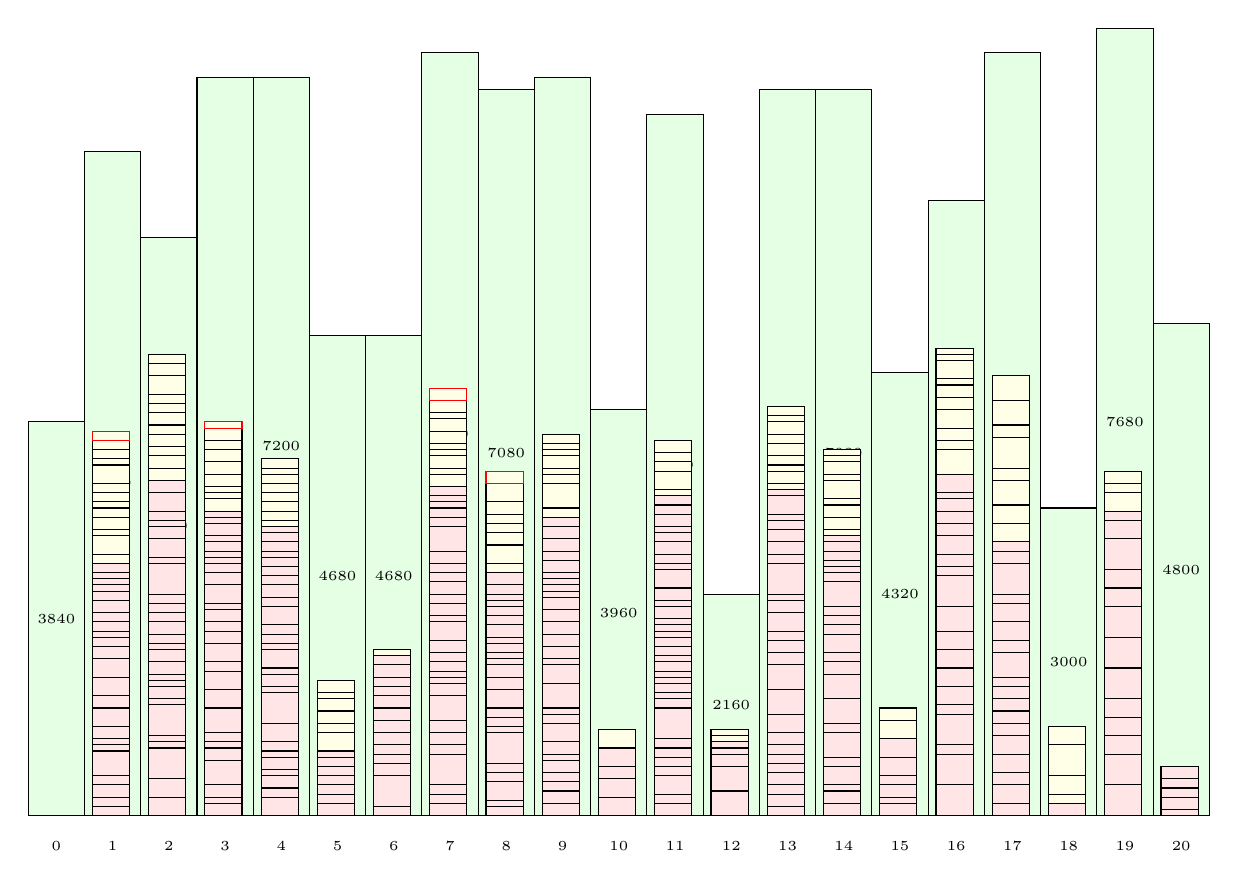
\begin{tikzpicture}[xscale=1.000000,yscale=1.000000]
\node[below] () at (0.357143,-0.2) {\tiny 0};
\node[below] () at (1.071429,-0.2) {\tiny 1};
\node[below] () at (1.785714,-0.2) {\tiny 2};
\node[below] () at (2.500000,-0.2) {\tiny 3};
\node[below] () at (3.214286,-0.2) {\tiny 4};
\node[below] () at (3.928571,-0.2) {\tiny 5};
\node[below] () at (4.642857,-0.2) {\tiny 6};
\node[below] () at (5.357143,-0.2) {\tiny 7};
\node[below] () at (6.071429,-0.2) {\tiny 8};
\node[below] () at (6.785714,-0.2) {\tiny 9};
\node[below] () at (7.500000,-0.2) {\tiny 10};
\node[below] () at (8.214286,-0.2) {\tiny 11};
\node[below] () at (8.928571,-0.2) {\tiny 12};
\node[below] () at (9.642857,-0.2) {\tiny 13};
\node[below] () at (10.357143,-0.2) {\tiny 14};
\node[below] () at (11.071429,-0.2) {\tiny 15};
\node[below] () at (11.785714,-0.2) {\tiny 16};
\node[below] () at (12.500000,-0.2) {\tiny 17};
\node[below] () at (13.214286,-0.2) {\tiny 18};
\node[below] () at (13.928571,-0.2) {\tiny 19};
\node[below] () at (14.642857,-0.2) {\tiny 20};
\draw[draw=black,fill=green!10] (0.000000,0.000000) rectangle node {\tiny 3840} (0.714286,5.000000);
\draw[draw=black,fill=green!10] (0.714286,0.000000) rectangle node {\tiny 6480} (1.428571,8.437500);
\draw[fill=red!10] (0.814286,0.000000) rectangle node {\tiny } (1.285714,0.117188);
\draw[fill=red!10] (0.814286,0.117188) rectangle node {\tiny } (1.285714,0.234375);
\draw[fill=red!10] (0.814286,0.234375) rectangle node {\tiny } (1.285714,0.390625);
\draw[fill=red!10] (0.814286,0.390625) rectangle node {\tiny } (1.285714,0.507813);
\draw[fill=red!10] (0.814286,0.507813) rectangle node {\tiny } (1.285714,0.820313);
\draw[fill=red!10] (0.814286,0.820313) rectangle node {\tiny } (1.285714,0.898438);
\draw[fill=red!10] (0.814286,0.898438) rectangle node {\tiny } (1.285714,0.976563);
\draw[fill=red!10] (0.814286,0.976563) rectangle node {\tiny } (1.285714,1.132813);
\draw[fill=red!10] (0.814286,1.132813) rectangle node {\tiny } (1.285714,1.367188);
\draw[fill=red!10] (0.814286,1.367188) rectangle node {\tiny } (1.285714,1.523438);
\draw[fill=red!10] (0.814286,1.523438) rectangle node {\tiny } (1.285714,1.757813);
\draw[fill=red!10] (0.814286,1.757813) rectangle node {\tiny } (1.285714,1.992188);
\draw[fill=red!10] (0.814286,1.992188) rectangle node {\tiny } (1.285714,2.148438);
\draw[fill=red!10] (0.814286,2.148438) rectangle node {\tiny } (1.285714,2.265625);
\draw[fill=red!10] (0.814286,2.265625) rectangle node {\tiny } (1.285714,2.343750);
\draw[fill=red!10] (0.814286,2.343750) rectangle node {\tiny } (1.285714,2.460938);
\draw[fill=red!10] (0.814286,2.460938) rectangle node {\tiny } (1.285714,2.578125);
\draw[fill=red!10] (0.814286,2.578125) rectangle node {\tiny } (1.285714,2.734375);
\draw[fill=red!10] (0.814286,2.734375) rectangle node {\tiny } (1.285714,2.851563);
\draw[fill=red!10] (0.814286,2.851563) rectangle node {\tiny } (1.285714,2.929688);
\draw[fill=red!10] (0.814286,2.929688) rectangle node {\tiny } (1.285714,3.007813);
\draw[fill=red!10] (0.814286,3.007813) rectangle node {\tiny } (1.285714,3.085938);
\draw[fill=red!10] (0.814286,3.085938) rectangle node {\tiny } (1.285714,3.203125);
\draw[fill=yellow!10] (0.814286,3.203125) rectangle node {\tiny } (1.285714,3.320313);
\draw[fill=yellow!10] (0.814286,3.320313) rectangle node {\tiny } (1.285714,3.554688);
\draw[fill=yellow!10] (0.814286,3.554688) rectangle node {\tiny } (1.285714,3.632813);
\draw[fill=yellow!10] (0.814286,3.632813) rectangle node {\tiny } (1.285714,3.789063);
\draw[fill=yellow!10] (0.814286,3.789063) rectangle node {\tiny } (1.285714,3.906250);
\draw[fill=yellow!10] (0.814286,3.906250) rectangle node {\tiny } (1.285714,3.984375);
\draw[fill=yellow!10] (0.814286,3.984375) rectangle node {\tiny } (1.285714,4.101563);
\draw[fill=yellow!10] (0.814286,4.101563) rectangle node {\tiny } (1.285714,4.218750);
\draw[fill=yellow!10] (0.814286,4.218750) rectangle node {\tiny } (1.285714,4.453125);
\draw[fill=yellow!10] (0.814286,4.453125) rectangle node {\tiny } (1.285714,4.531250);
\draw[fill=yellow!10] (0.814286,4.531250) rectangle node {\tiny } (1.285714,4.648438);
\draw[fill=yellow!10] (0.814286,4.648438) rectangle node {\tiny } (1.285714,4.765625);
\draw[draw=red,fill=yellow!10] (0.814286,4.765625) rectangle node {\tiny } (1.285714,4.882813);
\draw[draw=black,fill=green!10] (1.428571,0.000000) rectangle node {\tiny 5640} (2.142857,7.343750);
\draw[fill=red!10] (1.528571,0.000000) rectangle node {\tiny } (2.000000,0.234375);
\draw[fill=red!10] (1.528571,0.234375) rectangle node {\tiny } (2.000000,0.468750);
\draw[fill=red!10] (1.528571,0.468750) rectangle node {\tiny } (2.000000,0.859375);
\draw[fill=red!10] (1.528571,0.859375) rectangle node {\tiny } (2.000000,0.937500);
\draw[fill=red!10] (1.528571,0.937500) rectangle node {\tiny } (2.000000,1.015625);
\draw[fill=red!10] (1.528571,1.015625) rectangle node {\tiny } (2.000000,1.406250);
\draw[fill=red!10] (1.528571,1.406250) rectangle node {\tiny } (2.000000,1.484375);
\draw[fill=red!10] (1.528571,1.484375) rectangle node {\tiny } (2.000000,1.640625);
\draw[fill=red!10] (1.528571,1.640625) rectangle node {\tiny } (2.000000,1.718750);
\draw[fill=red!10] (1.528571,1.718750) rectangle node {\tiny } (2.000000,1.796875);
\draw[fill=red!10] (1.528571,1.796875) rectangle node {\tiny } (2.000000,1.953125);
\draw[fill=red!10] (1.528571,1.953125) rectangle node {\tiny } (2.000000,2.109375);
\draw[fill=red!10] (1.528571,2.109375) rectangle node {\tiny } (2.000000,2.187500);
\draw[fill=red!10] (1.528571,2.187500) rectangle node {\tiny } (2.000000,2.304688);
\draw[fill=red!10] (1.528571,2.304688) rectangle node {\tiny } (2.000000,2.460938);
\draw[fill=red!10] (1.528571,2.460938) rectangle node {\tiny } (2.000000,2.578125);
\draw[fill=red!10] (1.528571,2.578125) rectangle node {\tiny } (2.000000,2.695313);
\draw[fill=red!10] (1.528571,2.695313) rectangle node {\tiny } (2.000000,2.812500);
\draw[fill=red!10] (1.528571,2.812500) rectangle node {\tiny } (2.000000,3.203125);
\draw[fill=red!10] (1.528571,3.203125) rectangle node {\tiny } (2.000000,3.281250);
\draw[fill=red!10] (1.528571,3.281250) rectangle node {\tiny } (2.000000,3.515625);
\draw[fill=red!10] (1.528571,3.515625) rectangle node {\tiny } (2.000000,3.671875);
\draw[fill=red!10] (1.528571,3.671875) rectangle node {\tiny } (2.000000,3.750000);
\draw[fill=red!10] (1.528571,3.750000) rectangle node {\tiny } (2.000000,3.867188);
\draw[fill=red!10] (1.528571,3.867188) rectangle node {\tiny } (2.000000,4.101563);
\draw[fill=red!10] (1.528571,4.101563) rectangle node {\tiny } (2.000000,4.257813);
\draw[fill=yellow!10] (1.528571,4.257813) rectangle node {\tiny } (2.000000,4.414063);
\draw[fill=yellow!10] (1.528571,4.414063) rectangle node {\tiny } (2.000000,4.570313);
\draw[fill=yellow!10] (1.528571,4.570313) rectangle node {\tiny } (2.000000,4.687500);
\draw[fill=yellow!10] (1.528571,4.687500) rectangle node {\tiny } (2.000000,4.843750);
\draw[fill=yellow!10] (1.528571,4.843750) rectangle node {\tiny } (2.000000,4.960938);
\draw[fill=yellow!10] (1.528571,4.960938) rectangle node {\tiny } (2.000000,5.117188);
\draw[fill=yellow!10] (1.528571,5.117188) rectangle node {\tiny } (2.000000,5.234375);
\draw[fill=yellow!10] (1.528571,5.234375) rectangle node {\tiny } (2.000000,5.351563);
\draw[fill=yellow!10] (1.528571,5.351563) rectangle node {\tiny } (2.000000,5.585938);
\draw[fill=yellow!10] (1.528571,5.585938) rectangle node {\tiny } (2.000000,5.742188);
\draw[fill=yellow!10] (1.528571,5.742188) rectangle node {\tiny } (2.000000,5.859375);
\draw[draw=black,fill=green!10] (2.142857,0.000000) rectangle node {\tiny 7200} (2.857143,9.375000);
\draw[fill=red!10] (2.242857,0.000000) rectangle node {\tiny } (2.714286,0.156250);
\draw[fill=red!10] (2.242857,0.156250) rectangle node {\tiny } (2.714286,0.234375);
\draw[fill=red!10] (2.242857,0.234375) rectangle node {\tiny } (2.714286,0.390625);
\draw[fill=red!10] (2.242857,0.390625) rectangle node {\tiny } (2.714286,0.703125);
\draw[fill=red!10] (2.242857,0.703125) rectangle node {\tiny } (2.714286,0.859375);
\draw[fill=red!10] (2.242857,0.859375) rectangle node {\tiny } (2.714286,0.937500);
\draw[fill=red!10] (2.242857,0.937500) rectangle node {\tiny } (2.714286,1.054688);
\draw[fill=red!10] (2.242857,1.054688) rectangle node {\tiny } (2.714286,1.367188);
\draw[fill=red!10] (2.242857,1.367188) rectangle node {\tiny } (2.714286,1.601563);
\draw[fill=red!10] (2.242857,1.601563) rectangle node {\tiny } (2.714286,1.835938);
\draw[fill=red!10] (2.242857,1.835938) rectangle node {\tiny } (2.714286,1.953125);
\draw[fill=red!10] (2.242857,1.953125) rectangle node {\tiny } (2.714286,2.187500);
\draw[fill=red!10] (2.242857,2.187500) rectangle node {\tiny } (2.714286,2.343750);
\draw[fill=red!10] (2.242857,2.343750) rectangle node {\tiny } (2.714286,2.460938);
\draw[fill=red!10] (2.242857,2.460938) rectangle node {\tiny } (2.714286,2.617188);
\draw[fill=red!10] (2.242857,2.617188) rectangle node {\tiny } (2.714286,2.695313);
\draw[fill=red!10] (2.242857,2.695313) rectangle node {\tiny } (2.714286,2.929688);
\draw[fill=red!10] (2.242857,2.929688) rectangle node {\tiny } (2.714286,3.085938);
\draw[fill=red!10] (2.242857,3.085938) rectangle node {\tiny } (2.714286,3.203125);
\draw[fill=red!10] (2.242857,3.203125) rectangle node {\tiny } (2.714286,3.281250);
\draw[fill=red!10] (2.242857,3.281250) rectangle node {\tiny } (2.714286,3.359375);
\draw[fill=red!10] (2.242857,3.359375) rectangle node {\tiny } (2.714286,3.476563);
\draw[fill=red!10] (2.242857,3.476563) rectangle node {\tiny } (2.714286,3.554688);
\draw[fill=red!10] (2.242857,3.554688) rectangle node {\tiny } (2.714286,3.710938);
\draw[fill=red!10] (2.242857,3.710938) rectangle node {\tiny } (2.714286,3.789063);
\draw[fill=red!10] (2.242857,3.789063) rectangle node {\tiny } (2.714286,3.867188);
\draw[fill=yellow!10] (2.242857,3.867188) rectangle node {\tiny } (2.714286,4.023438);
\draw[fill=yellow!10] (2.242857,4.023438) rectangle node {\tiny } (2.714286,4.101563);
\draw[fill=yellow!10] (2.242857,4.101563) rectangle node {\tiny } (2.714286,4.179688);
\draw[fill=yellow!10] (2.242857,4.179688) rectangle node {\tiny } (2.714286,4.335938);
\draw[fill=yellow!10] (2.242857,4.335938) rectangle node {\tiny } (2.714286,4.492188);
\draw[fill=yellow!10] (2.242857,4.492188) rectangle node {\tiny } (2.714286,4.648438);
\draw[fill=yellow!10] (2.242857,4.648438) rectangle node {\tiny } (2.714286,4.765625);
\draw[fill=yellow!10] (2.242857,4.765625) rectangle node {\tiny } (2.714286,4.921875);
\draw[draw=red,fill=yellow!10] (2.242857,4.921875) rectangle node {\tiny } (2.714286,5.000000);
\draw[draw=black,fill=green!10] (2.857143,0.000000) rectangle node {\tiny 7200} (3.571429,9.375000);
\draw[fill=red!10] (2.957143,0.000000) rectangle node {\tiny } (3.428571,0.234375);
\draw[fill=red!10] (2.957143,0.234375) rectangle node {\tiny } (3.428571,0.351563);
\draw[fill=red!10] (2.957143,0.351563) rectangle node {\tiny } (3.428571,0.507813);
\draw[fill=red!10] (2.957143,0.507813) rectangle node {\tiny } (3.428571,0.585938);
\draw[fill=red!10] (2.957143,0.585938) rectangle node {\tiny } (3.428571,0.742188);
\draw[fill=red!10] (2.957143,0.742188) rectangle node {\tiny } (3.428571,0.820313);
\draw[fill=red!10] (2.957143,0.820313) rectangle node {\tiny } (3.428571,0.937500);
\draw[fill=red!10] (2.957143,0.937500) rectangle node {\tiny } (3.428571,1.171875);
\draw[fill=red!10] (2.957143,1.171875) rectangle node {\tiny } (3.428571,1.562500);
\draw[fill=red!10] (2.957143,1.562500) rectangle node {\tiny } (3.428571,1.640625);
\draw[fill=red!10] (2.957143,1.640625) rectangle node {\tiny } (3.428571,1.796875);
\draw[fill=red!10] (2.957143,1.796875) rectangle node {\tiny } (3.428571,1.875000);
\draw[fill=red!10] (2.957143,1.875000) rectangle node {\tiny } (3.428571,2.109375);
\draw[fill=red!10] (2.957143,2.109375) rectangle node {\tiny } (3.428571,2.187500);
\draw[fill=red!10] (2.957143,2.187500) rectangle node {\tiny } (3.428571,2.304688);
\draw[fill=red!10] (2.957143,2.304688) rectangle node {\tiny } (3.428571,2.421875);
\draw[fill=red!10] (2.957143,2.421875) rectangle node {\tiny } (3.428571,2.656250);
\draw[fill=red!10] (2.957143,2.656250) rectangle node {\tiny } (3.428571,2.773438);
\draw[fill=red!10] (2.957143,2.773438) rectangle node {\tiny } (3.428571,2.929688);
\draw[fill=red!10] (2.957143,2.929688) rectangle node {\tiny } (3.428571,3.046875);
\draw[fill=red!10] (2.957143,3.046875) rectangle node {\tiny } (3.428571,3.164063);
\draw[fill=red!10] (2.957143,3.164063) rectangle node {\tiny } (3.428571,3.281250);
\draw[fill=red!10] (2.957143,3.281250) rectangle node {\tiny } (3.428571,3.359375);
\draw[fill=red!10] (2.957143,3.359375) rectangle node {\tiny } (3.428571,3.476563);
\draw[fill=red!10] (2.957143,3.476563) rectangle node {\tiny } (3.428571,3.593750);
\draw[fill=red!10] (2.957143,3.593750) rectangle node {\tiny } (3.428571,3.671875);
\draw[fill=yellow!10] (2.957143,3.671875) rectangle node {\tiny } (3.428571,3.750000);
\draw[fill=yellow!10] (2.957143,3.750000) rectangle node {\tiny } (3.428571,3.867188);
\draw[fill=yellow!10] (2.957143,3.867188) rectangle node {\tiny } (3.428571,3.984375);
\draw[fill=yellow!10] (2.957143,3.984375) rectangle node {\tiny } (3.428571,4.101563);
\draw[fill=yellow!10] (2.957143,4.101563) rectangle node {\tiny } (3.428571,4.218750);
\draw[fill=yellow!10] (2.957143,4.218750) rectangle node {\tiny } (3.428571,4.335938);
\draw[fill=yellow!10] (2.957143,4.335938) rectangle node {\tiny } (3.428571,4.414063);
\draw[fill=yellow!10] (2.957143,4.414063) rectangle node {\tiny } (3.428571,4.531250);
\draw[draw=black,fill=green!10] (3.571429,0.000000) rectangle node {\tiny 4680} (4.285714,6.093750);
\draw[fill=red!10] (3.671429,0.000000) rectangle node {\tiny } (4.142857,0.156250);
\draw[fill=red!10] (3.671429,0.156250) rectangle node {\tiny } (4.142857,0.273438);
\draw[fill=red!10] (3.671429,0.273438) rectangle node {\tiny } (4.142857,0.390625);
\draw[fill=red!10] (3.671429,0.390625) rectangle node {\tiny } (4.142857,0.507813);
\draw[fill=red!10] (3.671429,0.507813) rectangle node {\tiny } (4.142857,0.625000);
\draw[fill=red!10] (3.671429,0.625000) rectangle node {\tiny } (4.142857,0.742188);
\draw[fill=red!10] (3.671429,0.742188) rectangle node {\tiny } (4.142857,0.820313);
\draw[fill=yellow!10] (3.671429,0.820313) rectangle node {\tiny } (4.142857,1.054688);
\draw[fill=yellow!10] (3.671429,1.054688) rectangle node {\tiny } (4.142857,1.171875);
\draw[fill=yellow!10] (3.671429,1.171875) rectangle node {\tiny } (4.142857,1.328125);
\draw[fill=yellow!10] (3.671429,1.328125) rectangle node {\tiny } (4.142857,1.484375);
\draw[fill=yellow!10] (3.671429,1.484375) rectangle node {\tiny } (4.142857,1.562500);
\draw[fill=yellow!10] (3.671429,1.562500) rectangle node {\tiny } (4.142857,1.718750);
\draw[draw=black,fill=green!10] (4.285714,0.000000) rectangle node {\tiny 4680} (5.000000,6.093750);
\draw[fill=red!10] (4.385714,0.000000) rectangle node {\tiny } (4.857143,0.117188);
\draw[fill=red!10] (4.385714,0.117188) rectangle node {\tiny } (4.857143,0.507813);
\draw[fill=red!10] (4.385714,0.507813) rectangle node {\tiny } (4.857143,0.664063);
\draw[fill=red!10] (4.385714,0.664063) rectangle node {\tiny } (4.857143,0.781250);
\draw[fill=red!10] (4.385714,0.781250) rectangle node {\tiny } (4.857143,0.898438);
\draw[fill=red!10] (4.385714,0.898438) rectangle node {\tiny } (4.857143,1.054688);
\draw[fill=red!10] (4.385714,1.054688) rectangle node {\tiny } (4.857143,1.210938);
\draw[fill=red!10] (4.385714,1.210938) rectangle node {\tiny } (4.857143,1.367188);
\draw[fill=red!10] (4.385714,1.367188) rectangle node {\tiny } (4.857143,1.523438);
\draw[fill=red!10] (4.385714,1.523438) rectangle node {\tiny } (4.857143,1.640625);
\draw[fill=red!10] (4.385714,1.640625) rectangle node {\tiny } (4.857143,1.757813);
\draw[fill=red!10] (4.385714,1.757813) rectangle node {\tiny } (4.857143,1.914063);
\draw[fill=red!10] (4.385714,1.914063) rectangle node {\tiny } (4.857143,2.031250);
\draw[fill=yellow!10] (4.385714,2.031250) rectangle node {\tiny } (4.857143,2.109375);
\draw[draw=black,fill=green!10] (5.000000,0.000000) rectangle node {\tiny 7440} (5.714286,9.687500);
\draw[fill=red!10] (5.100000,0.000000) rectangle node {\tiny } (5.571429,0.156250);
\draw[fill=red!10] (5.100000,0.156250) rectangle node {\tiny } (5.571429,0.273438);
\draw[fill=red!10] (5.100000,0.273438) rectangle node {\tiny } (5.571429,0.390625);
\draw[fill=red!10] (5.100000,0.390625) rectangle node {\tiny } (5.571429,0.781250);
\draw[fill=red!10] (5.100000,0.781250) rectangle node {\tiny } (5.571429,0.898438);
\draw[fill=red!10] (5.100000,0.898438) rectangle node {\tiny } (5.571429,1.054688);
\draw[fill=red!10] (5.100000,1.054688) rectangle node {\tiny } (5.571429,1.210938);
\draw[fill=red!10] (5.100000,1.210938) rectangle node {\tiny } (5.571429,1.523438);
\draw[fill=red!10] (5.100000,1.523438) rectangle node {\tiny } (5.571429,1.679688);
\draw[fill=red!10] (5.100000,1.679688) rectangle node {\tiny } (5.571429,1.757813);
\draw[fill=red!10] (5.100000,1.757813) rectangle node {\tiny } (5.571429,1.835938);
\draw[fill=red!10] (5.100000,1.835938) rectangle node {\tiny } (5.571429,1.953125);
\draw[fill=red!10] (5.100000,1.953125) rectangle node {\tiny } (5.571429,2.070313);
\draw[fill=red!10] (5.100000,2.070313) rectangle node {\tiny } (5.571429,2.226563);
\draw[fill=red!10] (5.100000,2.226563) rectangle node {\tiny } (5.571429,2.460938);
\draw[fill=red!10] (5.100000,2.460938) rectangle node {\tiny } (5.571429,2.539063);
\draw[fill=red!10] (5.100000,2.539063) rectangle node {\tiny } (5.571429,2.695313);
\draw[fill=red!10] (5.100000,2.695313) rectangle node {\tiny } (5.571429,2.812500);
\draw[fill=red!10] (5.100000,2.812500) rectangle node {\tiny } (5.571429,2.968750);
\draw[fill=red!10] (5.100000,2.968750) rectangle node {\tiny } (5.571429,3.085938);
\draw[fill=red!10] (5.100000,3.085938) rectangle node {\tiny } (5.571429,3.203125);
\draw[fill=red!10] (5.100000,3.203125) rectangle node {\tiny } (5.571429,3.359375);
\draw[fill=red!10] (5.100000,3.359375) rectangle node {\tiny } (5.571429,3.671875);
\draw[fill=red!10] (5.100000,3.671875) rectangle node {\tiny } (5.571429,3.789063);
\draw[fill=red!10] (5.100000,3.789063) rectangle node {\tiny } (5.571429,3.906250);
\draw[fill=red!10] (5.100000,3.906250) rectangle node {\tiny } (5.571429,3.984375);
\draw[fill=red!10] (5.100000,3.984375) rectangle node {\tiny } (5.571429,4.062500);
\draw[fill=red!10] (5.100000,4.062500) rectangle node {\tiny } (5.571429,4.179688);
\draw[fill=yellow!10] (5.100000,4.179688) rectangle node {\tiny } (5.571429,4.335938);
\draw[fill=yellow!10] (5.100000,4.335938) rectangle node {\tiny } (5.571429,4.414063);
\draw[fill=yellow!10] (5.100000,4.414063) rectangle node {\tiny } (5.571429,4.570313);
\draw[fill=yellow!10] (5.100000,4.570313) rectangle node {\tiny } (5.571429,4.648438);
\draw[fill=yellow!10] (5.100000,4.648438) rectangle node {\tiny } (5.571429,4.726563);
\draw[fill=yellow!10] (5.100000,4.726563) rectangle node {\tiny } (5.571429,4.882813);
\draw[fill=yellow!10] (5.100000,4.882813) rectangle node {\tiny } (5.571429,5.039063);
\draw[fill=yellow!10] (5.100000,5.039063) rectangle node {\tiny } (5.571429,5.117188);
\draw[fill=yellow!10] (5.100000,5.117188) rectangle node {\tiny } (5.571429,5.273438);
\draw[draw=red,fill=yellow!10] (5.100000,5.273438) rectangle node {\tiny } (5.571429,5.429688);
\draw[draw=black,fill=green!10] (5.714286,0.000000) rectangle node {\tiny 7080} (6.428571,9.218750);
\draw[fill=red!10] (5.814286,0.000000) rectangle node {\tiny } (6.285714,0.117188);
\draw[fill=red!10] (5.814286,0.117188) rectangle node {\tiny } (6.285714,0.195313);
\draw[fill=red!10] (5.814286,0.195313) rectangle node {\tiny } (6.285714,0.429688);
\draw[fill=red!10] (5.814286,0.429688) rectangle node {\tiny } (6.285714,0.546875);
\draw[fill=red!10] (5.814286,0.546875) rectangle node {\tiny } (6.285714,0.664063);
\draw[fill=red!10] (5.814286,0.664063) rectangle node {\tiny } (6.285714,1.054688);
\draw[fill=red!10] (5.814286,1.054688) rectangle node {\tiny } (6.285714,1.132813);
\draw[fill=red!10] (5.814286,1.132813) rectangle node {\tiny } (6.285714,1.250000);
\draw[fill=red!10] (5.814286,1.250000) rectangle node {\tiny } (6.285714,1.367188);
\draw[fill=red!10] (5.814286,1.367188) rectangle node {\tiny } (6.285714,1.601563);
\draw[fill=red!10] (5.814286,1.601563) rectangle node {\tiny } (6.285714,1.757813);
\draw[fill=red!10] (5.814286,1.757813) rectangle node {\tiny } (6.285714,1.914063);
\draw[fill=red!10] (5.814286,1.914063) rectangle node {\tiny } (6.285714,1.992188);
\draw[fill=red!10] (5.814286,1.992188) rectangle node {\tiny } (6.285714,2.070313);
\draw[fill=red!10] (5.814286,2.070313) rectangle node {\tiny } (6.285714,2.187500);
\draw[fill=red!10] (5.814286,2.187500) rectangle node {\tiny } (6.285714,2.265625);
\draw[fill=red!10] (5.814286,2.265625) rectangle node {\tiny } (6.285714,2.421875);
\draw[fill=red!10] (5.814286,2.421875) rectangle node {\tiny } (6.285714,2.539063);
\draw[fill=red!10] (5.814286,2.539063) rectangle node {\tiny } (6.285714,2.656250);
\draw[fill=red!10] (5.814286,2.656250) rectangle node {\tiny } (6.285714,2.734375);
\draw[fill=red!10] (5.814286,2.734375) rectangle node {\tiny } (6.285714,2.812500);
\draw[fill=red!10] (5.814286,2.812500) rectangle node {\tiny } (6.285714,2.929688);
\draw[fill=red!10] (5.814286,2.929688) rectangle node {\tiny } (6.285714,3.085938);
\draw[fill=yellow!10] (5.814286,3.085938) rectangle node {\tiny } (6.285714,3.203125);
\draw[fill=yellow!10] (5.814286,3.203125) rectangle node {\tiny } (6.285714,3.437500);
\draw[fill=yellow!10] (5.814286,3.437500) rectangle node {\tiny } (6.285714,3.593750);
\draw[fill=yellow!10] (5.814286,3.593750) rectangle node {\tiny } (6.285714,3.710938);
\draw[fill=yellow!10] (5.814286,3.710938) rectangle node {\tiny } (6.285714,3.828125);
\draw[fill=yellow!10] (5.814286,3.828125) rectangle node {\tiny } (6.285714,3.984375);
\draw[fill=yellow!10] (5.814286,3.984375) rectangle node {\tiny } (6.285714,4.218750);
\draw[draw=red,fill=yellow!10] (5.814286,4.218750) rectangle node {\tiny } (6.285714,4.375000);
\draw[draw=black,fill=green!10] (6.428571,0.000000) rectangle node {\tiny 7200} (7.142857,9.375000);
\draw[fill=red!10] (6.528571,0.000000) rectangle node {\tiny } (7.000000,0.156250);
\draw[fill=red!10] (6.528571,0.156250) rectangle node {\tiny } (7.000000,0.312500);
\draw[fill=red!10] (6.528571,0.312500) rectangle node {\tiny } (7.000000,0.429688);
\draw[fill=red!10] (6.528571,0.429688) rectangle node {\tiny } (7.000000,0.546875);
\draw[fill=red!10] (6.528571,0.546875) rectangle node {\tiny } (7.000000,0.703125);
\draw[fill=red!10] (6.528571,0.703125) rectangle node {\tiny } (7.000000,0.781250);
\draw[fill=red!10] (6.528571,0.781250) rectangle node {\tiny } (7.000000,0.937500);
\draw[fill=red!10] (6.528571,0.937500) rectangle node {\tiny } (7.000000,1.171875);
\draw[fill=red!10] (6.528571,1.171875) rectangle node {\tiny } (7.000000,1.289063);
\draw[fill=red!10] (6.528571,1.289063) rectangle node {\tiny } (7.000000,1.367188);
\draw[fill=red!10] (6.528571,1.367188) rectangle node {\tiny } (7.000000,1.679688);
\draw[fill=red!10] (6.528571,1.679688) rectangle node {\tiny } (7.000000,1.914063);
\draw[fill=red!10] (6.528571,1.914063) rectangle node {\tiny } (7.000000,1.992188);
\draw[fill=red!10] (6.528571,1.992188) rectangle node {\tiny } (7.000000,2.148438);
\draw[fill=red!10] (6.528571,2.148438) rectangle node {\tiny } (7.000000,2.304688);
\draw[fill=red!10] (6.528571,2.304688) rectangle node {\tiny } (7.000000,2.460938);
\draw[fill=red!10] (6.528571,2.460938) rectangle node {\tiny } (7.000000,2.617188);
\draw[fill=red!10] (6.528571,2.617188) rectangle node {\tiny } (7.000000,2.773438);
\draw[fill=red!10] (6.528571,2.773438) rectangle node {\tiny } (7.000000,2.851563);
\draw[fill=red!10] (6.528571,2.851563) rectangle node {\tiny } (7.000000,2.929688);
\draw[fill=red!10] (6.528571,2.929688) rectangle node {\tiny } (7.000000,3.007813);
\draw[fill=red!10] (6.528571,3.007813) rectangle node {\tiny } (7.000000,3.085938);
\draw[fill=red!10] (6.528571,3.085938) rectangle node {\tiny } (7.000000,3.242188);
\draw[fill=red!10] (6.528571,3.242188) rectangle node {\tiny } (7.000000,3.359375);
\draw[fill=red!10] (6.528571,3.359375) rectangle node {\tiny } (7.000000,3.515625);
\draw[fill=red!10] (6.528571,3.515625) rectangle node {\tiny } (7.000000,3.671875);
\draw[fill=red!10] (6.528571,3.671875) rectangle node {\tiny } (7.000000,3.789063);
\draw[fill=yellow!10] (6.528571,3.789063) rectangle node {\tiny } (7.000000,3.906250);
\draw[fill=yellow!10] (6.528571,3.906250) rectangle node {\tiny } (7.000000,4.218750);
\draw[fill=yellow!10] (6.528571,4.218750) rectangle node {\tiny } (7.000000,4.335938);
\draw[fill=yellow!10] (6.528571,4.335938) rectangle node {\tiny } (7.000000,4.414063);
\draw[fill=yellow!10] (6.528571,4.414063) rectangle node {\tiny } (7.000000,4.570313);
\draw[fill=yellow!10] (6.528571,4.570313) rectangle node {\tiny } (7.000000,4.648438);
\draw[fill=yellow!10] (6.528571,4.648438) rectangle node {\tiny } (7.000000,4.726563);
\draw[fill=yellow!10] (6.528571,4.726563) rectangle node {\tiny } (7.000000,4.843750);
\draw[draw=black,fill=green!10] (7.142857,0.000000) rectangle node {\tiny 3960} (7.857143,5.156250);
\draw[fill=red!10] (7.242857,0.000000) rectangle node {\tiny } (7.714286,0.234375);
\draw[fill=red!10] (7.242857,0.234375) rectangle node {\tiny } (7.714286,0.468750);
\draw[fill=red!10] (7.242857,0.468750) rectangle node {\tiny } (7.714286,0.625000);
\draw[fill=red!10] (7.242857,0.625000) rectangle node {\tiny } (7.714286,0.859375);
\draw[fill=yellow!10] (7.242857,0.859375) rectangle node {\tiny } (7.714286,1.093750);
\draw[draw=black,fill=green!10] (7.857143,0.000000) rectangle node {\tiny 6840} (8.571429,8.906250);
\draw[fill=red!10] (7.957143,0.000000) rectangle node {\tiny } (8.428571,0.156250);
\draw[fill=red!10] (7.957143,0.156250) rectangle node {\tiny } (8.428571,0.273438);
\draw[fill=red!10] (7.957143,0.273438) rectangle node {\tiny } (8.428571,0.507813);
\draw[fill=red!10] (7.957143,0.507813) rectangle node {\tiny } (8.428571,0.625000);
\draw[fill=red!10] (7.957143,0.625000) rectangle node {\tiny } (8.428571,0.742188);
\draw[fill=red!10] (7.957143,0.742188) rectangle node {\tiny } (8.428571,0.859375);
\draw[fill=red!10] (7.957143,0.859375) rectangle node {\tiny } (8.428571,0.976563);
\draw[fill=red!10] (7.957143,0.976563) rectangle node {\tiny } (8.428571,1.367188);
\draw[fill=red!10] (7.957143,1.367188) rectangle node {\tiny } (8.428571,1.484375);
\draw[fill=red!10] (7.957143,1.484375) rectangle node {\tiny } (8.428571,1.562500);
\draw[fill=red!10] (7.957143,1.562500) rectangle node {\tiny } (8.428571,1.679688);
\draw[fill=red!10] (7.957143,1.679688) rectangle node {\tiny } (8.428571,1.757813);
\draw[fill=red!10] (7.957143,1.757813) rectangle node {\tiny } (8.428571,1.835938);
\draw[fill=red!10] (7.957143,1.835938) rectangle node {\tiny } (8.428571,1.953125);
\draw[fill=red!10] (7.957143,1.953125) rectangle node {\tiny } (8.428571,2.031250);
\draw[fill=red!10] (7.957143,2.031250) rectangle node {\tiny } (8.428571,2.148438);
\draw[fill=red!10] (7.957143,2.148438) rectangle node {\tiny } (8.428571,2.265625);
\draw[fill=red!10] (7.957143,2.265625) rectangle node {\tiny } (8.428571,2.343750);
\draw[fill=red!10] (7.957143,2.343750) rectangle node {\tiny } (8.428571,2.421875);
\draw[fill=red!10] (7.957143,2.421875) rectangle node {\tiny } (8.428571,2.500000);
\draw[fill=red!10] (7.957143,2.500000) rectangle node {\tiny } (8.428571,2.656250);
\draw[fill=red!10] (7.957143,2.656250) rectangle node {\tiny } (8.428571,2.734375);
\draw[fill=red!10] (7.957143,2.734375) rectangle node {\tiny } (8.428571,2.890625);
\draw[fill=red!10] (7.957143,2.890625) rectangle node {\tiny } (8.428571,3.125000);
\draw[fill=red!10] (7.957143,3.125000) rectangle node {\tiny } (8.428571,3.203125);
\draw[fill=red!10] (7.957143,3.203125) rectangle node {\tiny } (8.428571,3.320313);
\draw[fill=red!10] (7.957143,3.320313) rectangle node {\tiny } (8.428571,3.476563);
\draw[fill=red!10] (7.957143,3.476563) rectangle node {\tiny } (8.428571,3.593750);
\draw[fill=red!10] (7.957143,3.593750) rectangle node {\tiny } (8.428571,3.671875);
\draw[fill=red!10] (7.957143,3.671875) rectangle node {\tiny } (8.428571,3.828125);
\draw[fill=red!10] (7.957143,3.828125) rectangle node {\tiny } (8.428571,3.945313);
\draw[fill=red!10] (7.957143,3.945313) rectangle node {\tiny } (8.428571,4.062500);
\draw[fill=yellow!10] (7.957143,4.062500) rectangle node {\tiny } (8.428571,4.140625);
\draw[fill=yellow!10] (7.957143,4.140625) rectangle node {\tiny } (8.428571,4.375000);
\draw[fill=yellow!10] (7.957143,4.375000) rectangle node {\tiny } (8.428571,4.492188);
\draw[fill=yellow!10] (7.957143,4.492188) rectangle node {\tiny } (8.428571,4.609375);
\draw[fill=yellow!10] (7.957143,4.609375) rectangle node {\tiny } (8.428571,4.765625);
\draw[draw=black,fill=green!10] (8.571429,0.000000) rectangle node {\tiny 2160} (9.285714,2.812500);
\draw[fill=red!10] (8.671429,0.000000) rectangle node {\tiny } (9.142857,0.312500);
\draw[fill=red!10] (8.671429,0.312500) rectangle node {\tiny } (9.142857,0.625000);
\draw[fill=red!10] (8.671429,0.625000) rectangle node {\tiny } (9.142857,0.781250);
\draw[fill=red!10] (8.671429,0.781250) rectangle node {\tiny } (9.142857,0.859375);
\draw[fill=red!10] (8.671429,0.859375) rectangle node {\tiny } (9.142857,0.937500);
\draw[fill=yellow!10] (8.671429,0.937500) rectangle node {\tiny } (9.142857,1.015625);
\draw[fill=yellow!10] (8.671429,1.015625) rectangle node {\tiny } (9.142857,1.093750);
\draw[draw=black,fill=green!10] (9.285714,0.000000) rectangle node {\tiny 7080} (10.000000,9.218750);
\draw[fill=red!10] (9.385714,0.000000) rectangle node {\tiny } (9.857143,0.117188);
\draw[fill=red!10] (9.385714,0.117188) rectangle node {\tiny } (9.857143,0.273438);
\draw[fill=red!10] (9.385714,0.273438) rectangle node {\tiny } (9.857143,0.390625);
\draw[fill=red!10] (9.385714,0.390625) rectangle node {\tiny } (9.857143,0.546875);
\draw[fill=red!10] (9.385714,0.546875) rectangle node {\tiny } (9.857143,0.664063);
\draw[fill=red!10] (9.385714,0.664063) rectangle node {\tiny } (9.857143,0.781250);
\draw[fill=red!10] (9.385714,0.781250) rectangle node {\tiny } (9.857143,0.898438);
\draw[fill=red!10] (9.385714,0.898438) rectangle node {\tiny } (9.857143,1.054688);
\draw[fill=red!10] (9.385714,1.054688) rectangle node {\tiny } (9.857143,1.289063);
\draw[fill=red!10] (9.385714,1.289063) rectangle node {\tiny } (9.857143,1.601563);
\draw[fill=red!10] (9.385714,1.601563) rectangle node {\tiny } (9.857143,1.914063);
\draw[fill=red!10] (9.385714,1.914063) rectangle node {\tiny } (9.857143,2.070313);
\draw[fill=red!10] (9.385714,2.070313) rectangle node {\tiny } (9.857143,2.226563);
\draw[fill=red!10] (9.385714,2.226563) rectangle node {\tiny } (9.857143,2.343750);
\draw[fill=red!10] (9.385714,2.343750) rectangle node {\tiny } (9.857143,2.578125);
\draw[fill=red!10] (9.385714,2.578125) rectangle node {\tiny } (9.857143,2.734375);
\draw[fill=red!10] (9.385714,2.734375) rectangle node {\tiny } (9.857143,2.812500);
\draw[fill=red!10] (9.385714,2.812500) rectangle node {\tiny } (9.857143,3.203125);
\draw[fill=red!10] (9.385714,3.203125) rectangle node {\tiny } (9.857143,3.320313);
\draw[fill=red!10] (9.385714,3.320313) rectangle node {\tiny } (9.857143,3.476563);
\draw[fill=red!10] (9.385714,3.476563) rectangle node {\tiny } (9.857143,3.632813);
\draw[fill=red!10] (9.385714,3.632813) rectangle node {\tiny } (9.857143,3.750000);
\draw[fill=red!10] (9.385714,3.750000) rectangle node {\tiny } (9.857143,3.828125);
\draw[fill=red!10] (9.385714,3.828125) rectangle node {\tiny } (9.857143,4.062500);
\draw[fill=red!10] (9.385714,4.062500) rectangle node {\tiny } (9.857143,4.140625);
\draw[fill=yellow!10] (9.385714,4.140625) rectangle node {\tiny } (9.857143,4.218750);
\draw[fill=yellow!10] (9.385714,4.218750) rectangle node {\tiny } (9.857143,4.375000);
\draw[fill=yellow!10] (9.385714,4.375000) rectangle node {\tiny } (9.857143,4.453125);
\draw[fill=yellow!10] (9.385714,4.453125) rectangle node {\tiny } (9.857143,4.570313);
\draw[fill=yellow!10] (9.385714,4.570313) rectangle node {\tiny } (9.857143,4.726563);
\draw[fill=yellow!10] (9.385714,4.726563) rectangle node {\tiny } (9.857143,4.843750);
\draw[fill=yellow!10] (9.385714,4.843750) rectangle node {\tiny } (9.857143,5.000000);
\draw[fill=yellow!10] (9.385714,5.000000) rectangle node {\tiny } (9.857143,5.078125);
\draw[fill=yellow!10] (9.385714,5.078125) rectangle node {\tiny } (9.857143,5.195313);
\draw[draw=black,fill=green!10] (10.000000,0.000000) rectangle node {\tiny 7080} (10.714286,9.218750);
\draw[fill=red!10] (10.100000,0.000000) rectangle node {\tiny } (10.571429,0.156250);
\draw[fill=red!10] (10.100000,0.156250) rectangle node {\tiny } (10.571429,0.312500);
\draw[fill=red!10] (10.100000,0.312500) rectangle node {\tiny } (10.571429,0.390625);
\draw[fill=red!10] (10.100000,0.390625) rectangle node {\tiny } (10.571429,0.625000);
\draw[fill=red!10] (10.100000,0.625000) rectangle node {\tiny } (10.571429,0.742188);
\draw[fill=red!10] (10.100000,0.742188) rectangle node {\tiny } (10.571429,1.054688);
\draw[fill=red!10] (10.100000,1.054688) rectangle node {\tiny } (10.571429,1.171875);
\draw[fill=red!10] (10.100000,1.171875) rectangle node {\tiny } (10.571429,1.484375);
\draw[fill=red!10] (10.100000,1.484375) rectangle node {\tiny } (10.571429,1.796875);
\draw[fill=red!10] (10.100000,1.796875) rectangle node {\tiny } (10.571429,1.953125);
\draw[fill=red!10] (10.100000,1.953125) rectangle node {\tiny } (10.571429,2.070313);
\draw[fill=red!10] (10.100000,2.070313) rectangle node {\tiny } (10.571429,2.304688);
\draw[fill=red!10] (10.100000,2.304688) rectangle node {\tiny } (10.571429,2.421875);
\draw[fill=red!10] (10.100000,2.421875) rectangle node {\tiny } (10.571429,2.539063);
\draw[fill=red!10] (10.100000,2.539063) rectangle node {\tiny } (10.571429,2.656250);
\draw[fill=red!10] (10.100000,2.656250) rectangle node {\tiny } (10.571429,2.968750);
\draw[fill=red!10] (10.100000,2.968750) rectangle node {\tiny } (10.571429,3.085938);
\draw[fill=red!10] (10.100000,3.085938) rectangle node {\tiny } (10.571429,3.164063);
\draw[fill=red!10] (10.100000,3.164063) rectangle node {\tiny } (10.571429,3.242188);
\draw[fill=red!10] (10.100000,3.242188) rectangle node {\tiny } (10.571429,3.359375);
\draw[fill=red!10] (10.100000,3.359375) rectangle node {\tiny } (10.571429,3.476563);
\draw[fill=red!10] (10.100000,3.476563) rectangle node {\tiny } (10.571429,3.554688);
\draw[fill=yellow!10] (10.100000,3.554688) rectangle node {\tiny } (10.571429,3.632813);
\draw[fill=yellow!10] (10.100000,3.632813) rectangle node {\tiny } (10.571429,3.789063);
\draw[fill=yellow!10] (10.100000,3.789063) rectangle node {\tiny } (10.571429,3.945313);
\draw[fill=yellow!10] (10.100000,3.945313) rectangle node {\tiny } (10.571429,4.023438);
\draw[fill=yellow!10] (10.100000,4.023438) rectangle node {\tiny } (10.571429,4.257813);
\draw[fill=yellow!10] (10.100000,4.257813) rectangle node {\tiny } (10.571429,4.335938);
\draw[fill=yellow!10] (10.100000,4.335938) rectangle node {\tiny } (10.571429,4.492188);
\draw[fill=yellow!10] (10.100000,4.492188) rectangle node {\tiny } (10.571429,4.570313);
\draw[fill=yellow!10] (10.100000,4.570313) rectangle node {\tiny } (10.571429,4.648438);
\draw[draw=black,fill=green!10] (10.714286,0.000000) rectangle node {\tiny 4320} (11.428571,5.625000);
\draw[fill=red!10] (10.814286,0.000000) rectangle node {\tiny } (11.285714,0.156250);
\draw[fill=red!10] (10.814286,0.156250) rectangle node {\tiny } (11.285714,0.234375);
\draw[fill=red!10] (10.814286,0.234375) rectangle node {\tiny } (11.285714,0.390625);
\draw[fill=red!10] (10.814286,0.390625) rectangle node {\tiny } (11.285714,0.507813);
\draw[fill=red!10] (10.814286,0.507813) rectangle node {\tiny } (11.285714,0.742188);
\draw[fill=red!10] (10.814286,0.742188) rectangle node {\tiny } (11.285714,0.976563);
\draw[fill=yellow!10] (10.814286,0.976563) rectangle node {\tiny } (11.285714,1.210938);
\draw[fill=yellow!10] (10.814286,1.210938) rectangle node {\tiny } (11.285714,1.367188);
\draw[draw=black,fill=green!10] (11.428571,0.000000) rectangle node {\tiny 6000} (12.142857,7.812500);
\draw[fill=red!10] (11.528571,0.000000) rectangle node {\tiny } (12.000000,0.390625);
\draw[fill=red!10] (11.528571,0.390625) rectangle node {\tiny } (12.000000,0.781250);
\draw[fill=red!10] (11.528571,0.781250) rectangle node {\tiny } (12.000000,0.898438);
\draw[fill=red!10] (11.528571,0.898438) rectangle node {\tiny } (12.000000,1.289063);
\draw[fill=red!10] (11.528571,1.289063) rectangle node {\tiny } (12.000000,1.406250);
\draw[fill=red!10] (11.528571,1.406250) rectangle node {\tiny } (12.000000,1.640625);
\draw[fill=red!10] (11.528571,1.640625) rectangle node {\tiny } (12.000000,1.875000);
\draw[fill=red!10] (11.528571,1.875000) rectangle node {\tiny } (12.000000,2.109375);
\draw[fill=red!10] (11.528571,2.109375) rectangle node {\tiny } (12.000000,2.343750);
\draw[fill=red!10] (11.528571,2.343750) rectangle node {\tiny } (12.000000,2.656250);
\draw[fill=red!10] (11.528571,2.656250) rectangle node {\tiny } (12.000000,3.046875);
\draw[fill=red!10] (11.528571,3.046875) rectangle node {\tiny } (12.000000,3.164063);
\draw[fill=red!10] (11.528571,3.164063) rectangle node {\tiny } (12.000000,3.320313);
\draw[fill=red!10] (11.528571,3.320313) rectangle node {\tiny } (12.000000,3.554688);
\draw[fill=red!10] (11.528571,3.554688) rectangle node {\tiny } (12.000000,3.710938);
\draw[fill=red!10] (11.528571,3.710938) rectangle node {\tiny } (12.000000,3.867188);
\draw[fill=red!10] (11.528571,3.867188) rectangle node {\tiny } (12.000000,4.023438);
\draw[fill=red!10] (11.528571,4.023438) rectangle node {\tiny } (12.000000,4.101563);
\draw[fill=red!10] (11.528571,4.101563) rectangle node {\tiny } (12.000000,4.335938);
\draw[fill=yellow!10] (11.528571,4.335938) rectangle node {\tiny } (12.000000,4.648438);
\draw[fill=yellow!10] (11.528571,4.648438) rectangle node {\tiny } (12.000000,4.765625);
\draw[fill=yellow!10] (11.528571,4.765625) rectangle node {\tiny } (12.000000,4.921875);
\draw[fill=yellow!10] (11.528571,4.921875) rectangle node {\tiny } (12.000000,5.156250);
\draw[fill=yellow!10] (11.528571,5.156250) rectangle node {\tiny } (12.000000,5.312500);
\draw[fill=yellow!10] (11.528571,5.312500) rectangle node {\tiny } (12.000000,5.468750);
\draw[fill=yellow!10] (11.528571,5.468750) rectangle node {\tiny } (12.000000,5.546875);
\draw[fill=yellow!10] (11.528571,5.546875) rectangle node {\tiny } (12.000000,5.781250);
\draw[fill=yellow!10] (11.528571,5.781250) rectangle node {\tiny } (12.000000,5.859375);
\draw[fill=yellow!10] (11.528571,5.859375) rectangle node {\tiny } (12.000000,5.937500);
\draw[draw=black,fill=green!10] (12.142857,0.000000) rectangle node {\tiny 7440} (12.857143,9.687500);
\draw[fill=red!10] (12.242857,0.000000) rectangle node {\tiny } (12.714286,0.156250);
\draw[fill=red!10] (12.242857,0.156250) rectangle node {\tiny } (12.714286,0.390625);
\draw[fill=red!10] (12.242857,0.390625) rectangle node {\tiny } (12.714286,0.546875);
\draw[fill=red!10] (12.242857,0.546875) rectangle node {\tiny } (12.714286,0.781250);
\draw[fill=red!10] (12.242857,0.781250) rectangle node {\tiny } (12.714286,1.015625);
\draw[fill=red!10] (12.242857,1.015625) rectangle node {\tiny } (12.714286,1.171875);
\draw[fill=red!10] (12.242857,1.171875) rectangle node {\tiny } (12.714286,1.328125);
\draw[fill=red!10] (12.242857,1.328125) rectangle node {\tiny } (12.714286,1.484375);
\draw[fill=red!10] (12.242857,1.484375) rectangle node {\tiny } (12.714286,1.640625);
\draw[fill=red!10] (12.242857,1.640625) rectangle node {\tiny } (12.714286,1.757813);
\draw[fill=red!10] (12.242857,1.757813) rectangle node {\tiny } (12.714286,2.070313);
\draw[fill=red!10] (12.242857,2.070313) rectangle node {\tiny } (12.714286,2.226563);
\draw[fill=red!10] (12.242857,2.226563) rectangle node {\tiny } (12.714286,2.460938);
\draw[fill=red!10] (12.242857,2.460938) rectangle node {\tiny } (12.714286,2.695313);
\draw[fill=red!10] (12.242857,2.695313) rectangle node {\tiny } (12.714286,2.812500);
\draw[fill=red!10] (12.242857,2.812500) rectangle node {\tiny } (12.714286,3.203125);
\draw[fill=red!10] (12.242857,3.203125) rectangle node {\tiny } (12.714286,3.359375);
\draw[fill=red!10] (12.242857,3.359375) rectangle node {\tiny } (12.714286,3.476563);
\draw[fill=yellow!10] (12.242857,3.476563) rectangle node {\tiny } (12.714286,3.710938);
\draw[fill=yellow!10] (12.242857,3.710938) rectangle node {\tiny } (12.714286,3.945313);
\draw[fill=yellow!10] (12.242857,3.945313) rectangle node {\tiny } (12.714286,4.257813);
\draw[fill=yellow!10] (12.242857,4.257813) rectangle node {\tiny } (12.714286,4.414063);
\draw[fill=yellow!10] (12.242857,4.414063) rectangle node {\tiny } (12.714286,4.804688);
\draw[fill=yellow!10] (12.242857,4.804688) rectangle node {\tiny } (12.714286,4.960938);
\draw[fill=yellow!10] (12.242857,4.960938) rectangle node {\tiny } (12.714286,5.273438);
\draw[fill=yellow!10] (12.242857,5.273438) rectangle node {\tiny } (12.714286,5.585938);
\draw[draw=black,fill=green!10] (12.857143,0.000000) rectangle node {\tiny 3000} (13.571429,3.906250);
\draw[fill=red!10] (12.957143,0.000000) rectangle node {\tiny } (13.428571,0.156250);
\draw[fill=yellow!10] (12.957143,0.156250) rectangle node {\tiny } (13.428571,0.273438);
\draw[fill=yellow!10] (12.957143,0.273438) rectangle node {\tiny } (13.428571,0.507813);
\draw[fill=yellow!10] (12.957143,0.507813) rectangle node {\tiny } (13.428571,0.898438);
\draw[fill=yellow!10] (12.957143,0.898438) rectangle node {\tiny } (13.428571,1.132813);
\draw[draw=black,fill=green!10] (13.571429,0.000000) rectangle node {\tiny 7680} (14.285714,10.000000);
\draw[fill=red!10] (13.671429,0.000000) rectangle node {\tiny } (14.142857,0.390625);
\draw[fill=red!10] (13.671429,0.390625) rectangle node {\tiny } (14.142857,0.781250);
\draw[fill=red!10] (13.671429,0.781250) rectangle node {\tiny } (14.142857,1.015625);
\draw[fill=red!10] (13.671429,1.015625) rectangle node {\tiny } (14.142857,1.250000);
\draw[fill=red!10] (13.671429,1.250000) rectangle node {\tiny } (14.142857,1.484375);
\draw[fill=red!10] (13.671429,1.484375) rectangle node {\tiny } (14.142857,1.875000);
\draw[fill=red!10] (13.671429,1.875000) rectangle node {\tiny } (14.142857,2.265625);
\draw[fill=red!10] (13.671429,2.265625) rectangle node {\tiny } (14.142857,2.656250);
\draw[fill=red!10] (13.671429,2.656250) rectangle node {\tiny } (14.142857,2.890625);
\draw[fill=red!10] (13.671429,2.890625) rectangle node {\tiny } (14.142857,3.125000);
\draw[fill=red!10] (13.671429,3.125000) rectangle node {\tiny } (14.142857,3.515625);
\draw[fill=red!10] (13.671429,3.515625) rectangle node {\tiny } (14.142857,3.750000);
\draw[fill=red!10] (13.671429,3.750000) rectangle node {\tiny } (14.142857,3.867188);
\draw[fill=yellow!10] (13.671429,3.867188) rectangle node {\tiny } (14.142857,4.101563);
\draw[fill=yellow!10] (13.671429,4.101563) rectangle node {\tiny } (14.142857,4.218750);
\draw[fill=yellow!10] (13.671429,4.218750) rectangle node {\tiny } (14.142857,4.375000);
\draw[draw=black,fill=green!10] (14.285714,0.000000) rectangle node {\tiny 4800} (15.000000,6.250000);
\draw[fill=red!10] (14.385714,0.000000) rectangle node {\tiny } (14.857143,0.078125);
\draw[fill=red!10] (14.385714,0.078125) rectangle node {\tiny } (14.857143,0.234375);
\draw[fill=red!10] (14.385714,0.234375) rectangle node {\tiny } (14.857143,0.351563);
\draw[fill=red!10] (14.385714,0.351563) rectangle node {\tiny } (14.857143,0.468750);
\draw[fill=red!10] (14.385714,0.468750) rectangle node {\tiny } (14.857143,0.625000);
\end{tikzpicture}

}
\end{frame}


\begin{frame}
\frametitle{Process}
\begin{itemize}
\item We used this problem in a tutorial on modelling at CP 2025 in Glasgow 
\item Show different modelling and solution approaches
\item Developed in two weeks
\item Since then, further improved models for admission
\item Split cost into A (admission) and B (nursing)
\item Quite good results for cost A, not so good (yet) for cost B
\end{itemize}
\end{frame}

\begin{frame}
\frametitle{Cost Comparison A/B}
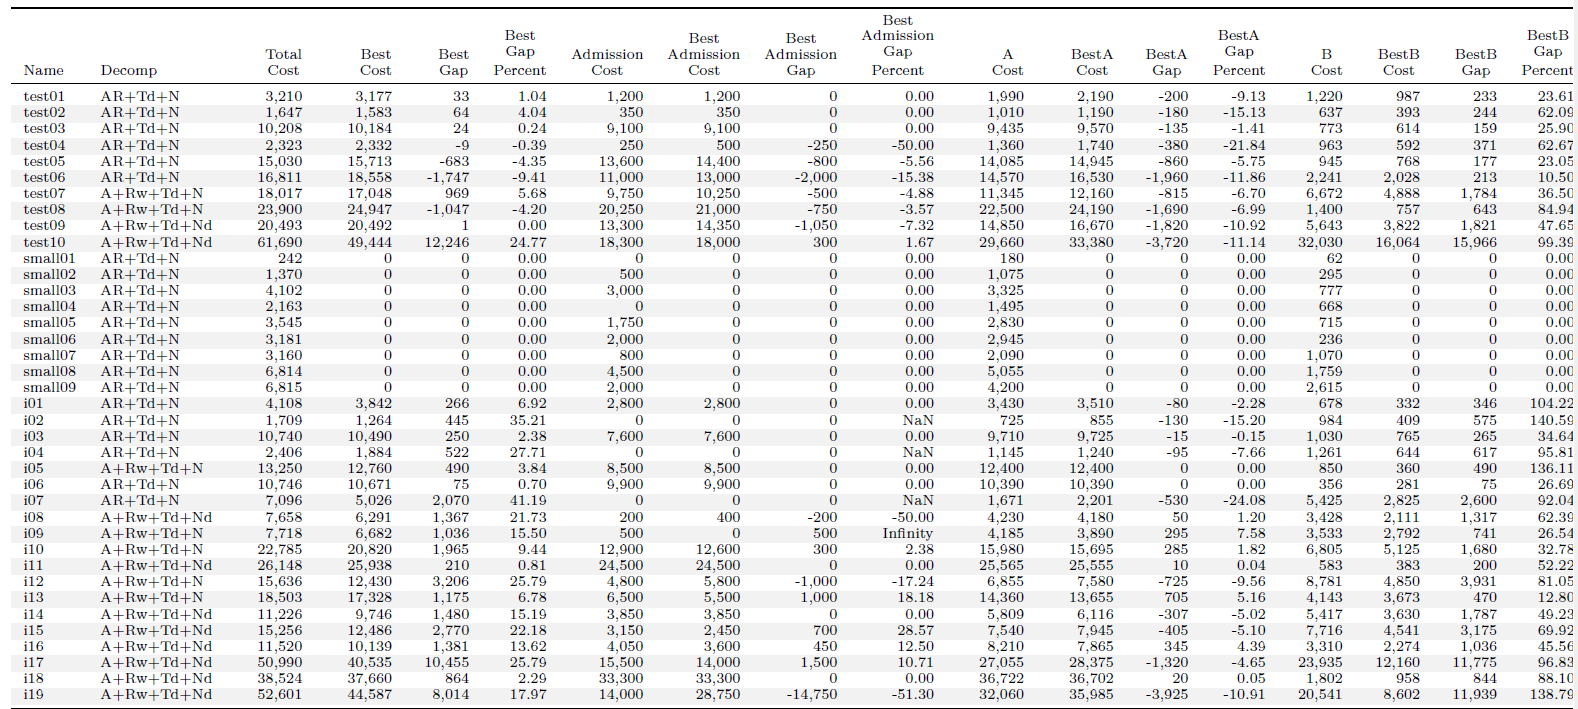
\includegraphics[width=\textwidth]{../schedulingseminar/ihtc2024/resultsab}
\end{frame}

% \begin{frame}
% \frametitle{Cost Comparison for Different Cost Terms}
% 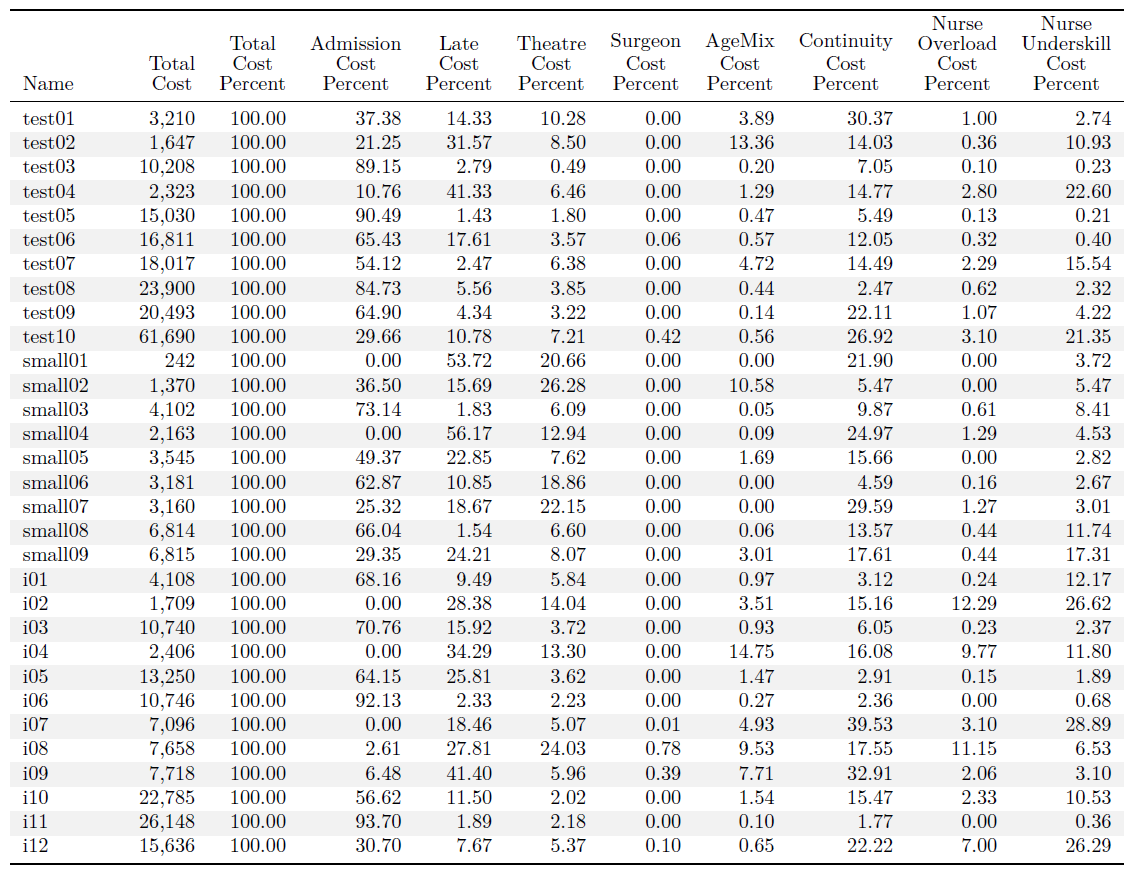
\includegraphics[width=.9\textwidth]{../schedulingseminar/ihtc2024/resultscostpercent}
% \end{frame}

\subsection{New Use Cases}

\begin{frame}
\frametitle{Which problem do we need to solve?}
\begin{itemize}
\item Competition is only concerned with generating initial solution
\item But there are many more use cases to study
\begin{itemize}
\item What happens if a rejected patient needs the operation now
\item What happens if a surgeon cancels a session
\item What happens if the hospital closes for a disaster event
\item What resources do we need to handle $k$ additional patients
\end{itemize}
\item This is linked to ongoing work on explanations in our lab
\end{itemize}
\end{frame}



\section{A Generic Scheduling Tool}

\begin{frame}
\frametitle{A Generic Scheduling Tool}
\begin{itemize}
\item Intended for ENTIRE customers, SME and PSO
\begin{itemize}
\item Smaller problem scope, very limited tech resources
\end{itemize}
\item No programming, configured by JSON input data
\item Compositional use of different constraint types
\item Different commercial or open-source back-end solvers
\item Developed in Java
\item Interactive JavaFX front-end
\item Can by used as back-end scheduling tool/server (REST)
\item Instance generator included
\item Readers for multiple benchmark types included
\end{itemize}
\end{frame}

\begin{frame}
\frametitle{Scheduling Tool GUI Examples}
\begin{tabular}{cc}
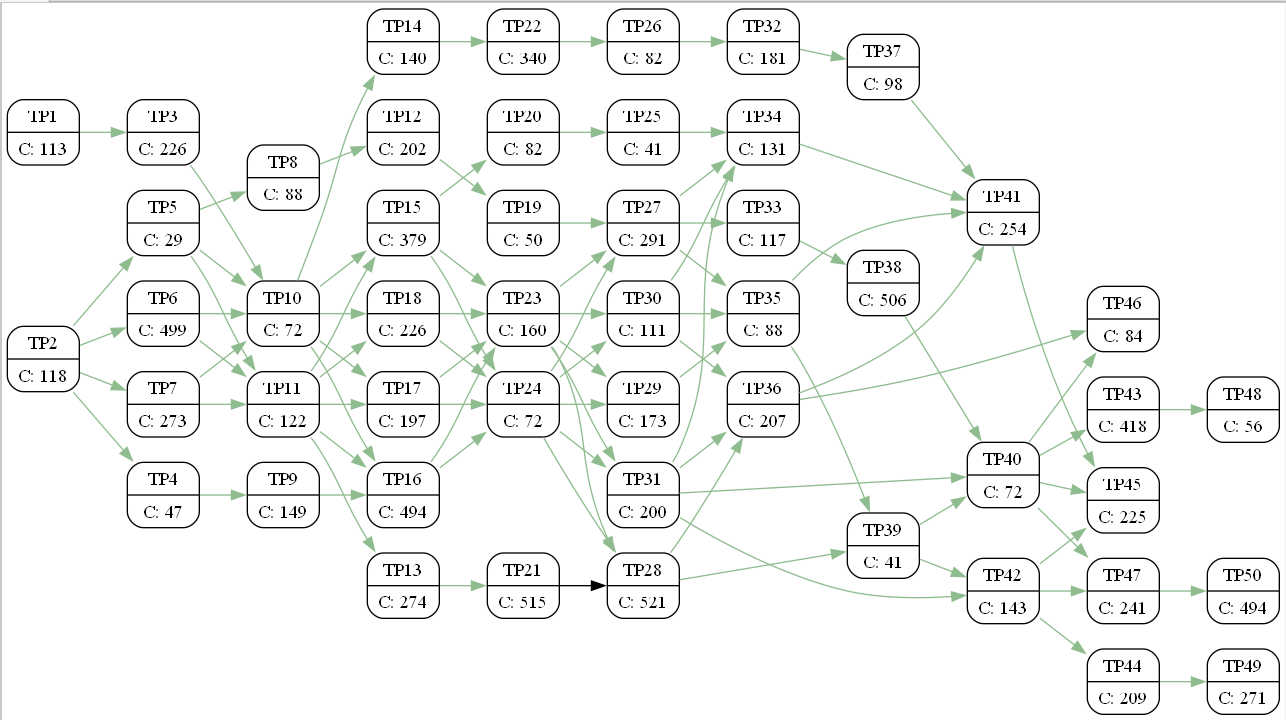
\includegraphics[width=.5\textwidth]{images/processchart}
&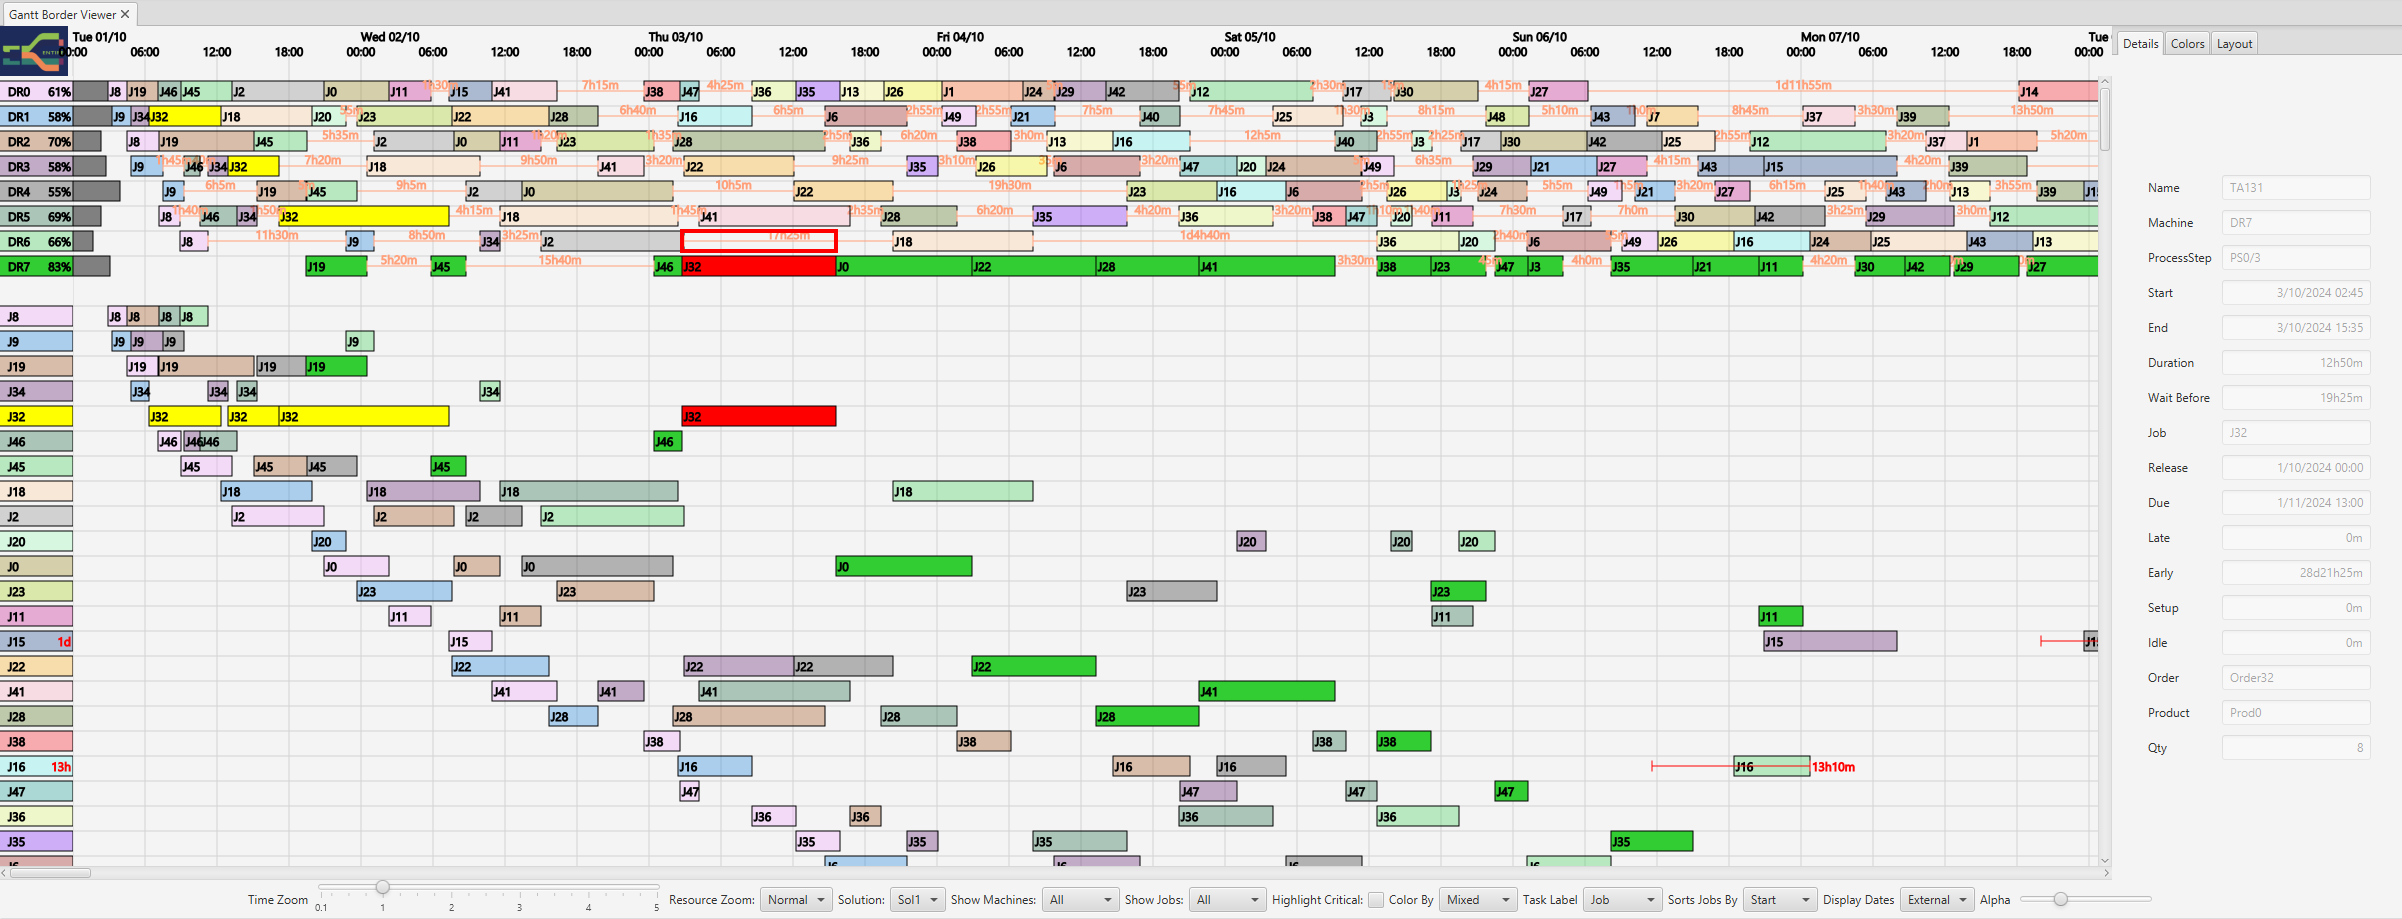
\includegraphics[width=.5\textwidth]{images/gantt}
\\

\includegraphics[width=.5\textwidth]{images/pert}
&
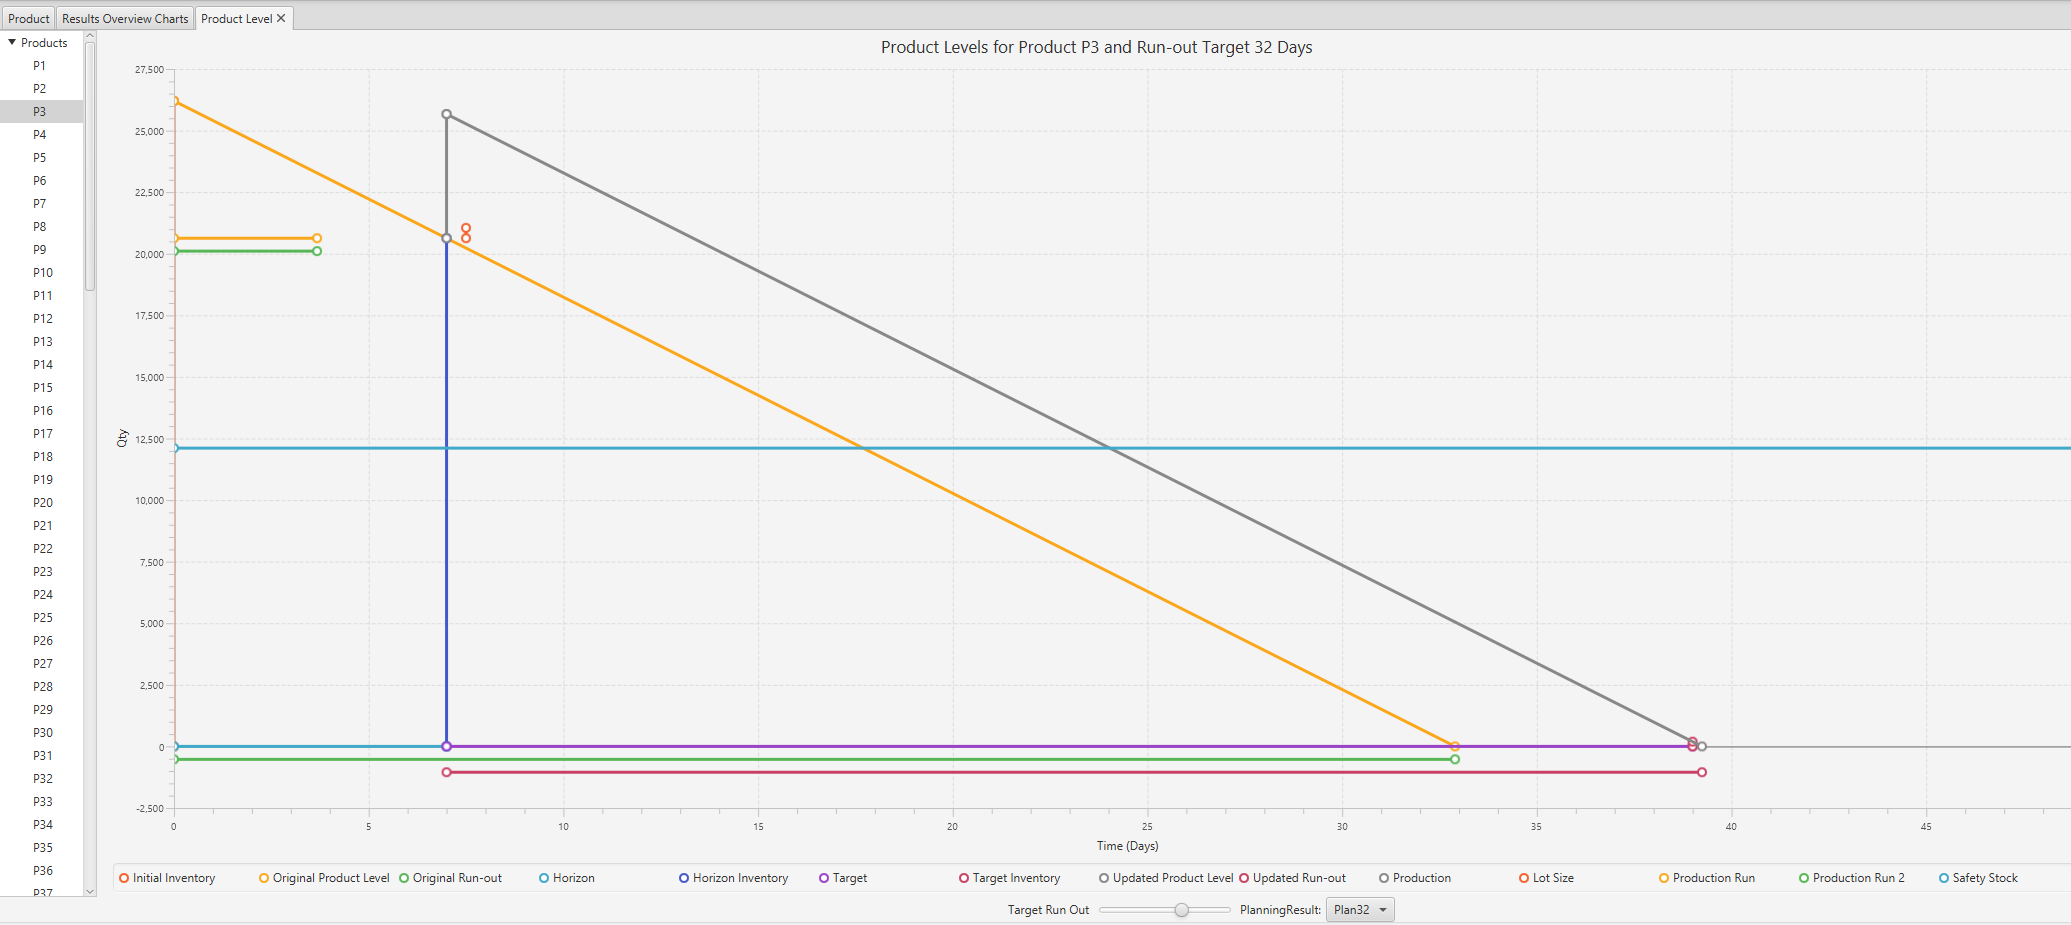
\includegraphics[width=.5\textwidth]{images/productionplanning}
\end{tabular}

\end{frame}

% \begin{frame}
% \frametitle{Key Points}
% \begin{itemize}
% \item This section describes the scheduling tool
% \begin{itemize}
% \item This is a \emph{preview} of the current state, not released yet!
% \end{itemize}
% \item How to load/create data
% \begin{itemize}
% \item From files
% \item By instance generator
% \item From benchmark problems
% \end{itemize}
% \item How to run the solvers
% \begin{itemize}
% \item Which solvers are supported
% \item What to expect in terms of performance
% \end{itemize}
% \item Experiments to try
% \begin{itemize}
% \item Limited time
% \item Possible "test before invest" continuation
% \end{itemize}

% \end{itemize}
% \end{frame}



\subsection{Under the hood}

\begin{frame}
\frametitle{Back-end solvers}
\begin{itemize}
\item Provide both open-source and commercial solver interfaces
\item Allow experimentation without having to buy commercial tools straightaway
\item Gives a level playing field to compare solvers and models
\item Provides out-of-the-box, generic performance
\end{itemize}
\end{frame}


\begin{frame}
\frametitle{Google OR-Tools CPSat Solver}
\begin{columns}
\begin{column}{0.5\textwidth}
\begin{itemize}
\item Open-Source tool provided by Google
\item Available at \url{https://developers.google.com/optimization/cp/cp_solver}
\item Probably best open-source CP solver for scheduling
\item This solver is packaged with scheduling tool
\end{itemize}
\end{column}
\begin{column}{0.5\textwidth}
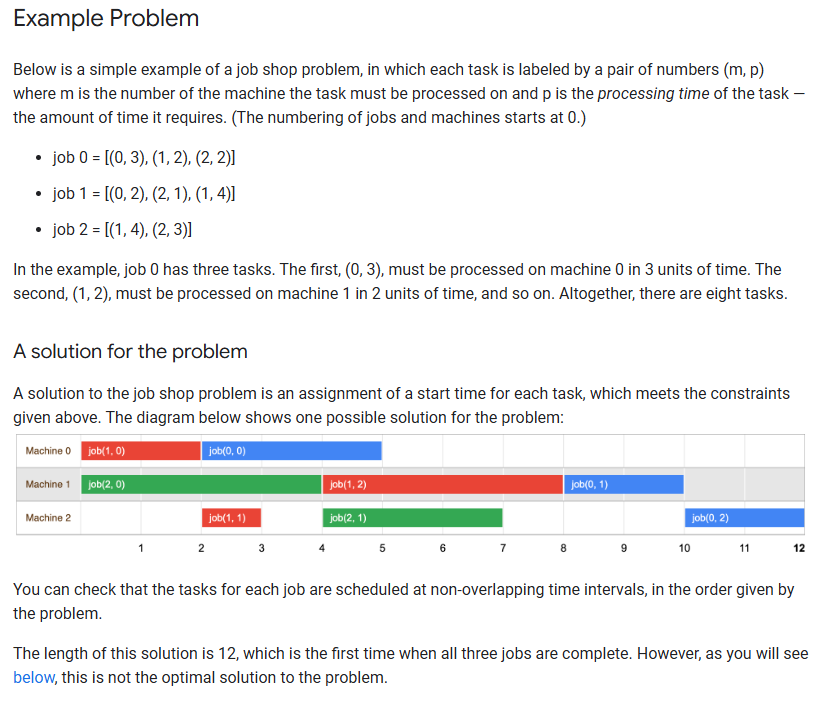
\includegraphics[width=\textwidth]{../04-experiments/images/cpsat-example}

{\tiny (from OR-Tools website)}
\end{column}
\end{columns}
\end{frame}

\begin{frame}
\frametitle{CP Optimizer from IBM}
\begin{columns}
\begin{column}{0.5\textwidth}
\begin{itemize}
\item Commercial tool of IBM
\item \url{https://www.ibm.com/products/ilog-cplex-optimization-studio/cplex-cp-optimizer}
\item Part of optimization suite with Cplex, OPL
\item We allow to interface with it
\item Academic licenses available
\item Well-known for capabilities for scheduling

\end{itemize}
\end{column}
\begin{column}{0.5\textwidth}
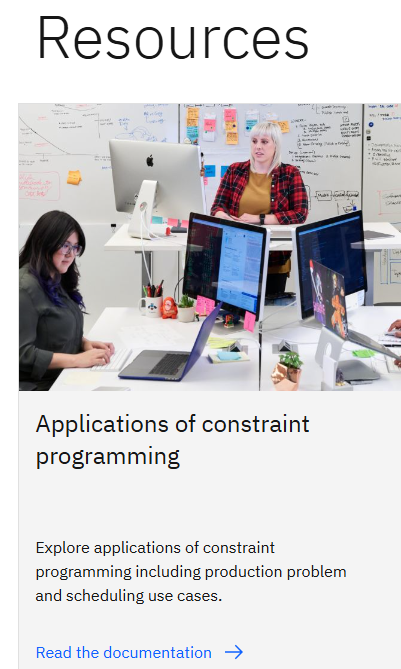
\includegraphics[width=.7\textwidth]{../04-experiments/images/cpoptimizer-example}

{\tiny (from CPOptimizer website)}
\end{column}
\end{columns}
\end{frame}


\begin{frame}
\frametitle{MiniZinc from Monash University}
\begin{columns}
\begin{column}{0.5\textwidth}
\begin{itemize}
\item Modelling language and backend tools from Monash University in Melbourne, Australia
\item Available from \url{https://www.minizinc.org/}
\item Widely used for teaching
\item Allows different backend solver to run from same model
\item Generic CP tool, not optimized for scheduling
\item Requires separate installation, open-source
\end{itemize}
\end{column}
\begin{column}{0.5\textwidth}
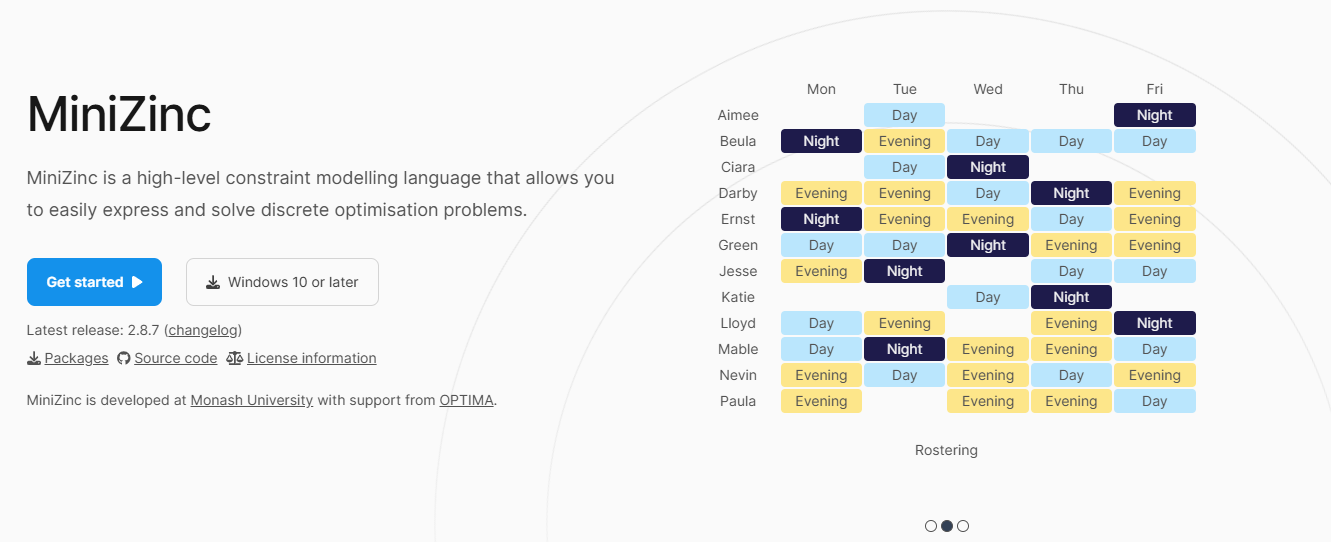
\includegraphics[width=\textwidth]{../04-experiments/images/minizinc-example}

{\tiny (from MiniZinc Website)}
\end{column}
\end{columns}
\end{frame}


\begin{frame}
\frametitle{Which Solver is Better?}
\begin{itemize}
\item We present results on a few benchmark types
\item Fair comparison between solvers
\begin{itemize}
\item Same hardware, Windows 11 laptop
\item CPU i7-10875H @ 2.3GHz, 64GB, four cores
\item Same timeout (600 s)
\end{itemize}
\item Not a fair comparison to state-of-the-art
\begin{itemize}
\item Uses out-of-the-box model
\item Significant improvements possible
\item More specific models
\item Parameter tuning
\item Unlimited runtime
\end{itemize}

\end{itemize}
\end{frame}

\begin{frame}
\frametitle{Taillard Job-Shop Benchmarks}
\scalebox{0.6}{
\begin{tabular}{lr*{10}{r}} \toprule
& &\multicolumn{4}{c}{All Instances} & \multicolumn{2}{c}{Optimal Only} & \multicolumn{4}{c}{Non Optimal Only}\\ 
& &\multicolumn{4}{c}{Optimal (\% of All Instances)} & \multicolumn{2}{c}{Time (\% of VB)} & \multicolumn{2}{c}{Cost (\% of VB)} & \multicolumn{2}{c}{Bound (\% of VB)}\\ 
Group & Nr & Both & CPO & CPSat & None & CPO & CPSat & CPO & CPSat & CPO & CPSat\\ \midrule
15/15 & 10 & 90.00 &  0.00 &  0.00 & 10.00 & 105.19 & 141.18 & 100.00 & 100.00 & 97.17 & 100.00 \\ 
20/15 & 10 & 20.00 &  0.00 &  0.00 & 80.00 & 267.27 & 263.20 & 100.99 & 100.05 & 98.50 & 99.93 \\ 
20/20 & 10 &  0.00 &  0.00 &  0.00 & 100.00 & n/a & n/a & 100.74 & 100.06 & 97.96 & 100.00 \\ 
30/15 & 10 & 10.00 &  0.00 & 10.00 & 80.00 & 174.32 & 100.00 & 100.18 & 100.49 & 99.87 & 100.00 \\ 
30/20 & 10 &  0.00 &  0.00 &  0.00 & 100.00 & n/a & n/a & 100.30 & 101.30 & 99.40 & 100.00 \\ 
50/15 & 10 & 100.00 &  0.00 &  0.00 &  0.00 & 100.00 & 685.09 & n/a & n/a & n/a & n/a \\ 
50/20 & 10 & 10.00 & 60.00 &  0.00 & 30.00 & 100.00 & 381.38 & 100.00 & 101.60 & 100.00 & 100.00 \\ 
100/20 & 10 & 10.00 & 90.00 &  0.00 &  0.00 & 100.00 & 416.13 & 100.00 & 101.73 & 100.00 & 66.81 \\ 
\bottomrule
\end{tabular}
}

\begin{itemize}
\item Significant number of problems solved to optimality in 600s
\item In terms of quality, solvers are quite similar
\item CPO wins in terms of solution times for larger instances
\end{itemize}

\end{frame}

\begin{frame}
\frametitle{Results for Hybrid Flexible Flow-Shop}
\scalebox{0.6}{
\begin{tabular}{lr*{10}{r}} \toprule
& &\multicolumn{4}{c}{All Instances} & \multicolumn{2}{c}{Optimal Only} & \multicolumn{4}{c}{Non Optimal Only}\\ 
& &\multicolumn{4}{c}{Optimal (\% of All Instances)} & \multicolumn{2}{c}{Time (\% of VB)} & \multicolumn{2}{c}{Cost (\% of VB)} & \multicolumn{2}{c}{Bound (\% of VB)}\\ 
Group & Nr & Both & CPO & CPSat & None & CPO & CPSat & CPO & CPSat & CPO & CPSat\\ \midrule
20 & 25 & 76.00 &  0.00 & 20.00 &  4.00 & 100.00 & 580.71 & 100.00 & 100.00 & 96.52 & 100.00 \\ 
25 & 25 & 80.00 &  0.00 &  8.00 & 12.00 & 101.65 & 238.02 & 100.00 & 100.37 & 97.67 & 100.00 \\ 
30 & 25 & 60.00 &  0.00 &  4.00 & 36.00 & 100.35 & 264.69 & 100.18 & 101.05 & 100.00 & 100.00 \\ 
40 & 25 &  4.00 & 16.00 &  0.00 & 80.00 & 100.00 & 2554.03 & 100.00 & 104.68 & 100.00 & 100.00 \\ 
50 & 25 &  0.00 &  4.00 &  0.00 & 96.00 & n/a & n/a & 100.00 & 107.87 & 100.00 & 100.00 \\ 
100 & 25 &  0.00 &  0.00 &  0.00 & 100.00 & n/a & n/a & 100.00 & 120.43 & 100.00 & 100.00 \\ 
200 & 25 &  0.00 &  0.00 &  0.00 & 100.00 & n/a & n/a & 100.00 & 188.60 & 100.00 & 100.00 \\ 
300 & 24 &  0.00 &  0.00 &  0.00 & 100.00 & n/a & n/a & 100.00 & 263.22 & 100.00 & 100.00 \\ 
400 & 25 &  0.00 &  0.00 &  0.00 & 100.00 & n/a & n/a & 100.00 & 246.34 & 100.00 & 100.00 \\ 
\bottomrule
\end{tabular}
}
\begin{itemize}
\item Only smaller/medium instances solved to optimality
\item For those problems, both solvers perform well
\item CPO significantly better on large instances
\item But: Best CP only result with SICStus Prolog (Armstrong et al, CP 2021)
\item Best overall result with NEH/CP hybrid (Garraffa et al, Comput. Oper. Res., 2025)
\end{itemize}
\end{frame}

\begin{frame}
\frametitle{General Recommendations}
\begin{itemize}
\item If you already have access to CPO, use it!
\item For new problem types, do an evaluation with CPSat first
\item Out of the box, CPO performs more consistently
\item May be easier to extend CPSat with your own research
\item Use multiple cores and memory to your advantage
\item OptalCP (see last talk) gave superb results on Siemens Energy test case
\end{itemize}
\end{frame}



\subsection{Input Data/ Result Output}

\begin{frame}
\frametitle{I/O: JSON Base Data}
\begin{columns}
\begin{column}{0.5\textwidth}
\begin{itemize}
\item Description of 
\begin{itemize}
\item Product
\item Process
\item DisjunctiveResource
\item CumulativeNeed
\item ProcessStep
\item ResourceNeed
\item CumulativeProfile
\item Problem
\item CumulativeResource
\item ProcessSequence
\end{itemize}
\end{itemize}
\end{column}
\begin{column}{0.4\textwidth}

\includegraphics[width=\textwidth]{../04-experiments/images/basedata}
\end{column}
\end{columns}
\end{frame}

\begin{frame}
\frametitle{Schedule Input Data}
\begin{columns}
\begin{column}{0.5\textwidth}
\begin{itemize}
\item Description of
\begin{itemize}
\item Downtime
\item Task (x2)
\item Job
\item Order
\item WiP
\end{itemize}
\end{itemize}
\end{column}
\begin{column}{0.5\textwidth}
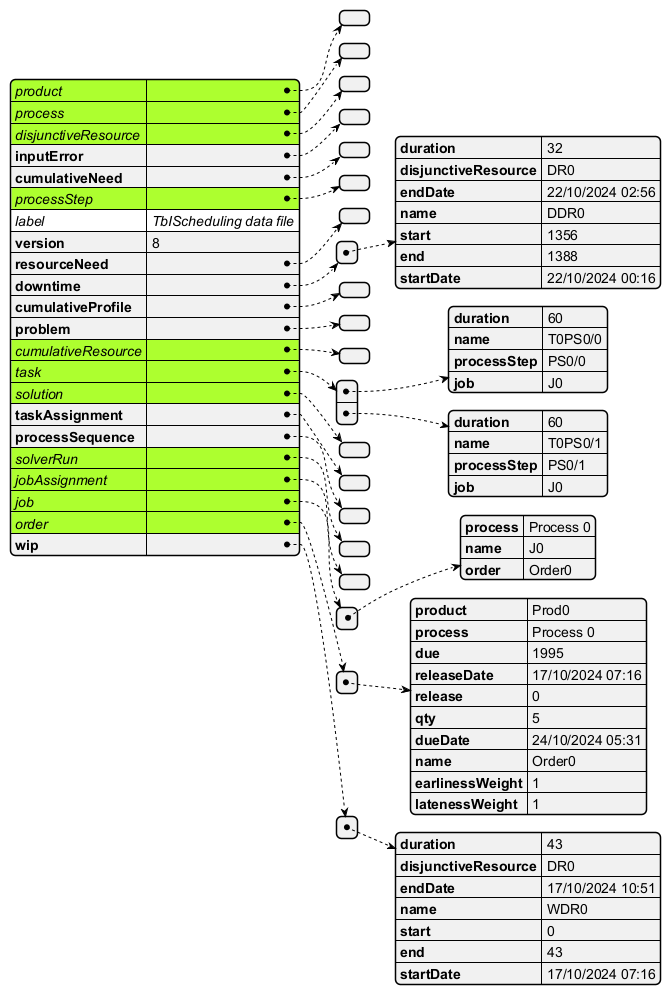
\includegraphics[width=\textwidth]{../04-experiments/images/schedule}
\end{column}
\end{columns}
\end{frame}



% \subsection{Result Output}

% \begin{frame}
% \frametitle{Result Data}
% \begin{itemize}
% \item We use the same JSON format to describe the results of the schedule
% \item Added field types for SolverRun, Solution, assigned Jobs and Tasks
% \end{itemize}
% \end{frame}

% \begin{frame}
% \frametitle{JSON Format Results}
% \begin{columns}
% \begin{column}{0.6\textwidth}
% \begin{itemize}
% \item Description of
% \begin{itemize}
% \item Solution
% \item SolverRun
% \item Job Assignment
% \item Task Assignment
% \end{itemize}

% \end{itemize}
% \end{column}
% \begin{column}{0.4\textwidth}
% 
\includegraphics[width=.7\textwidth]{../04-experiments/images/samplerresult}
% \end{column}
% \end{columns}
% \end{frame}



\subsection{Instance Generator}

\begin{frame}
\frametitle{Instance Generator}
\begin{itemize}
\item Application allows to generate different types of test problems
\item Different types of resource models
\item Different numbers of orders, resources, WiP, downtime
\item Useful to generate more life-like examples combining different constraint types
\end{itemize}
\end{frame}


\begin{frame}
\frametitle{Instance Generator Dialog}
\begin{columns}
\begin{column}{0.5\textwidth}
\begin{itemize}
\item Resource Model
\begin{itemize}
\item Select a resource model defining the overall structure of problem
\end{itemize}
\item Nr Disjunctive Resources
\begin{itemize}
\item Describe how many disjunctive resources are generated
\end{itemize}
\item Resource Probability
\begin{itemize}
\item The probability that a resource is compatible with a task
\item Only for some resource models
\end{itemize}
\end{itemize}
\end{column}
\begin{column}{0.5\textwidth}
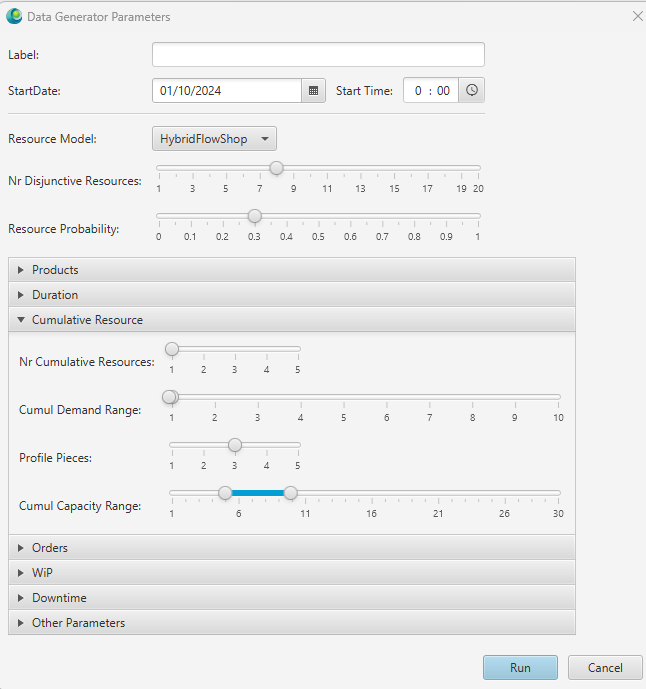
\includegraphics[width=\textwidth]{../04-experiments/images/instance-generator}
\end{column}
\end{columns}
\end{frame}

% \begin{frame}
% \frametitle{Resource Models}
% \begin{itemize}
% \item Flow-Shop
% \begin{itemize}
% \item Multiple stages, all jobs use machines in same order
% \end{itemize}

% \item Job-Shop
% \begin{itemize}
% \item Multiple stages, jobs use machines in different order
% \end{itemize}

% \item Open-Shop
% \begin{itemize}
% \item Multiple stages, no predefined order of machines
% \end{itemize}

% \item Hybrid Flow-Shop (default)
% \item Hybrid Job-Shop
% \item Hybrid Open-Shop
% \begin{itemize}
% \item Like x-shop, but with multiple machines per stage
% \end{itemize}

% \item Random
% \begin{itemize}
% \item Multiple stages, each stage using a random subset of machines
% \end{itemize}

% \item All
% \begin{itemize}
% \item Multiple stages, each stage allowing all machines
% \end{itemize}

% \end{itemize}
% \end{frame}



\begin{frame}
\frametitle{GUI: Example Job-Shop Solution}
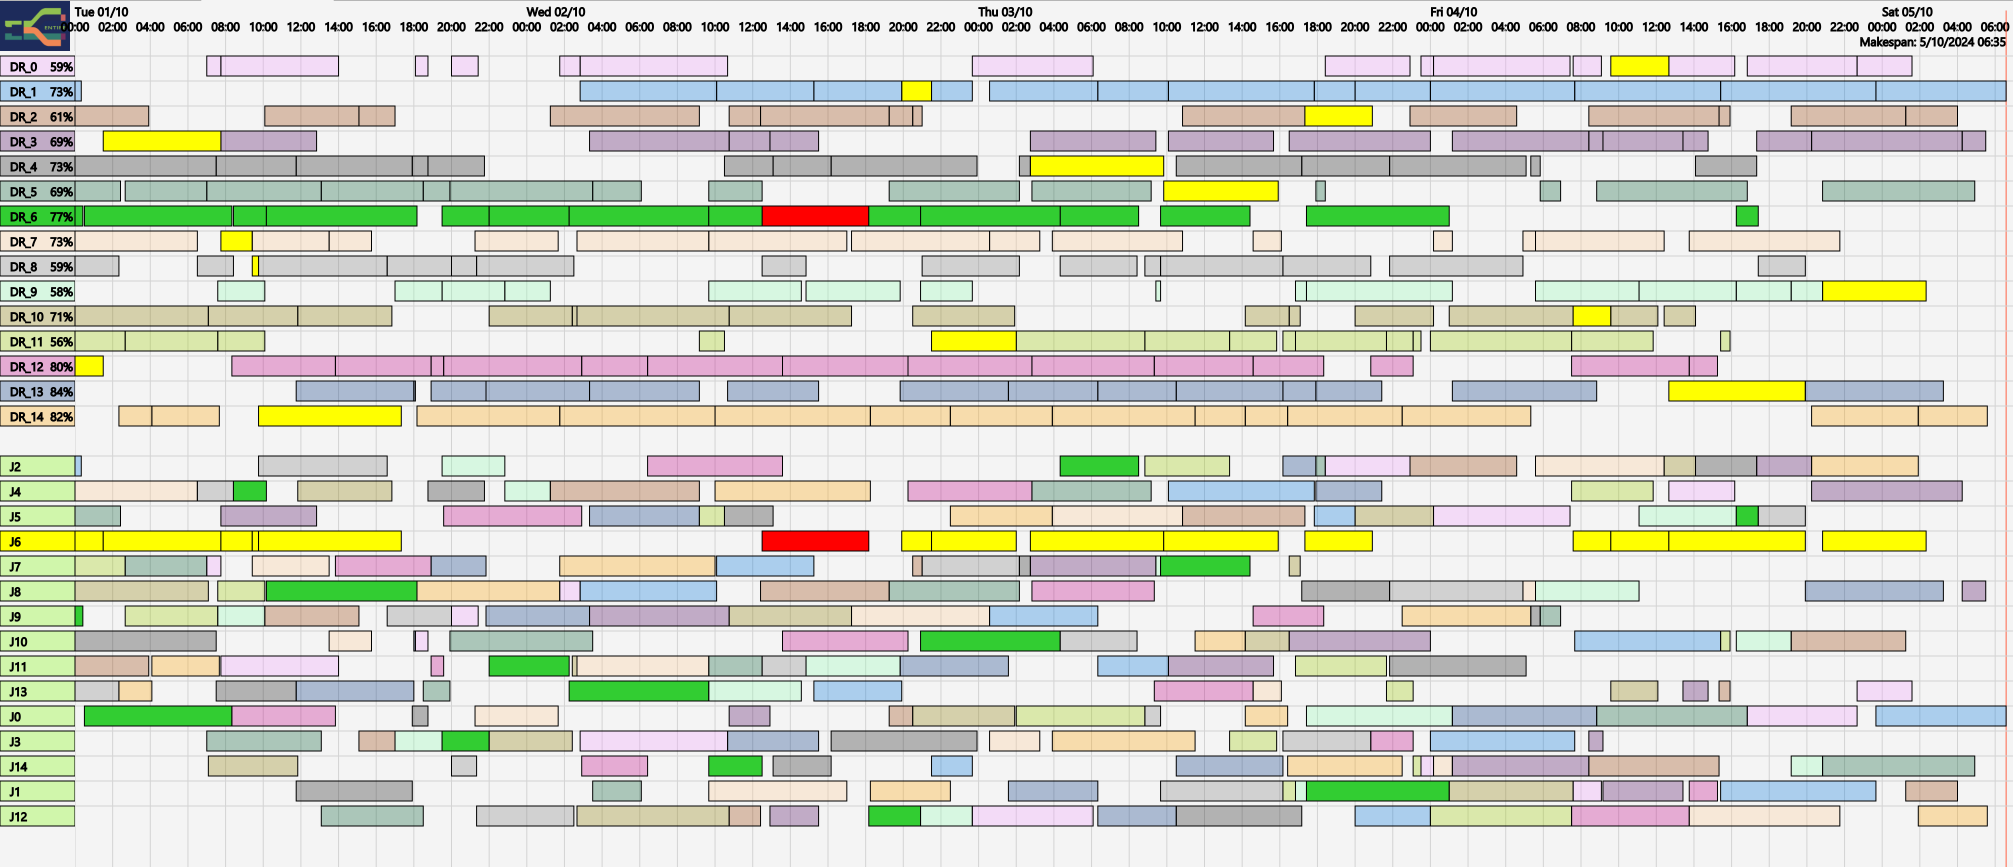
\includegraphics[width=\textwidth]{../02-concepts/images/job-shop-solution}

\begin{itemize}
\item One task is selected (in red), in both Machine and Job Gantt Chart
\item Tasks are colored by machine, note coloring in jobs is different for each job
\end{itemize}
\end{frame}


\begin{frame}
\frametitle{GUI: RCPSP Process Diagram}
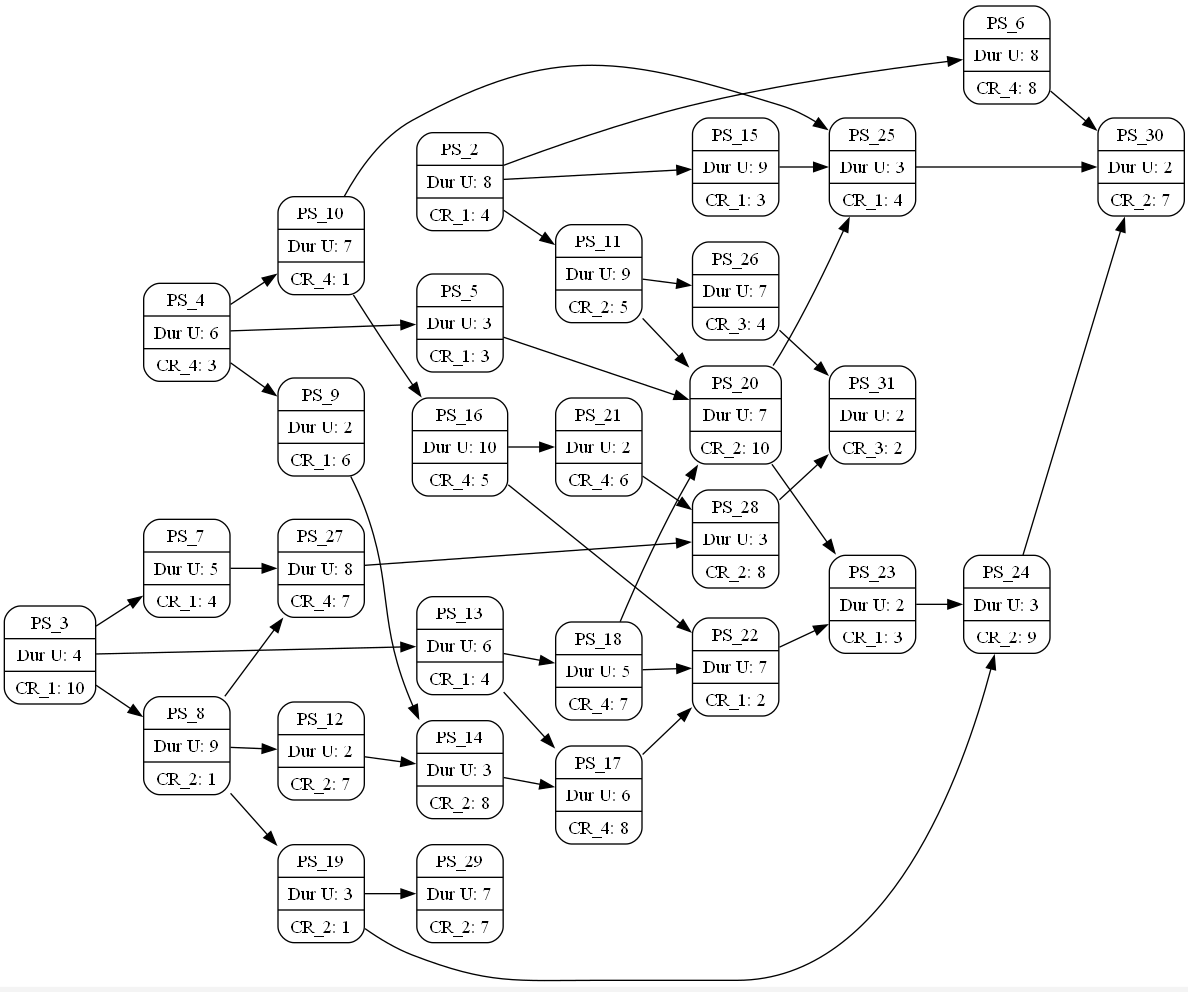
\includegraphics[width=.7\textwidth]{../02-concepts/images/rcpsp-process-diagram}
\begin{itemize}
\item Multiple sources, sinks
\item Multiple cumulative resources
\end{itemize}

\end{frame}

% \begin{frame}
% \frametitle{RCPSP PERT Diagram}
% 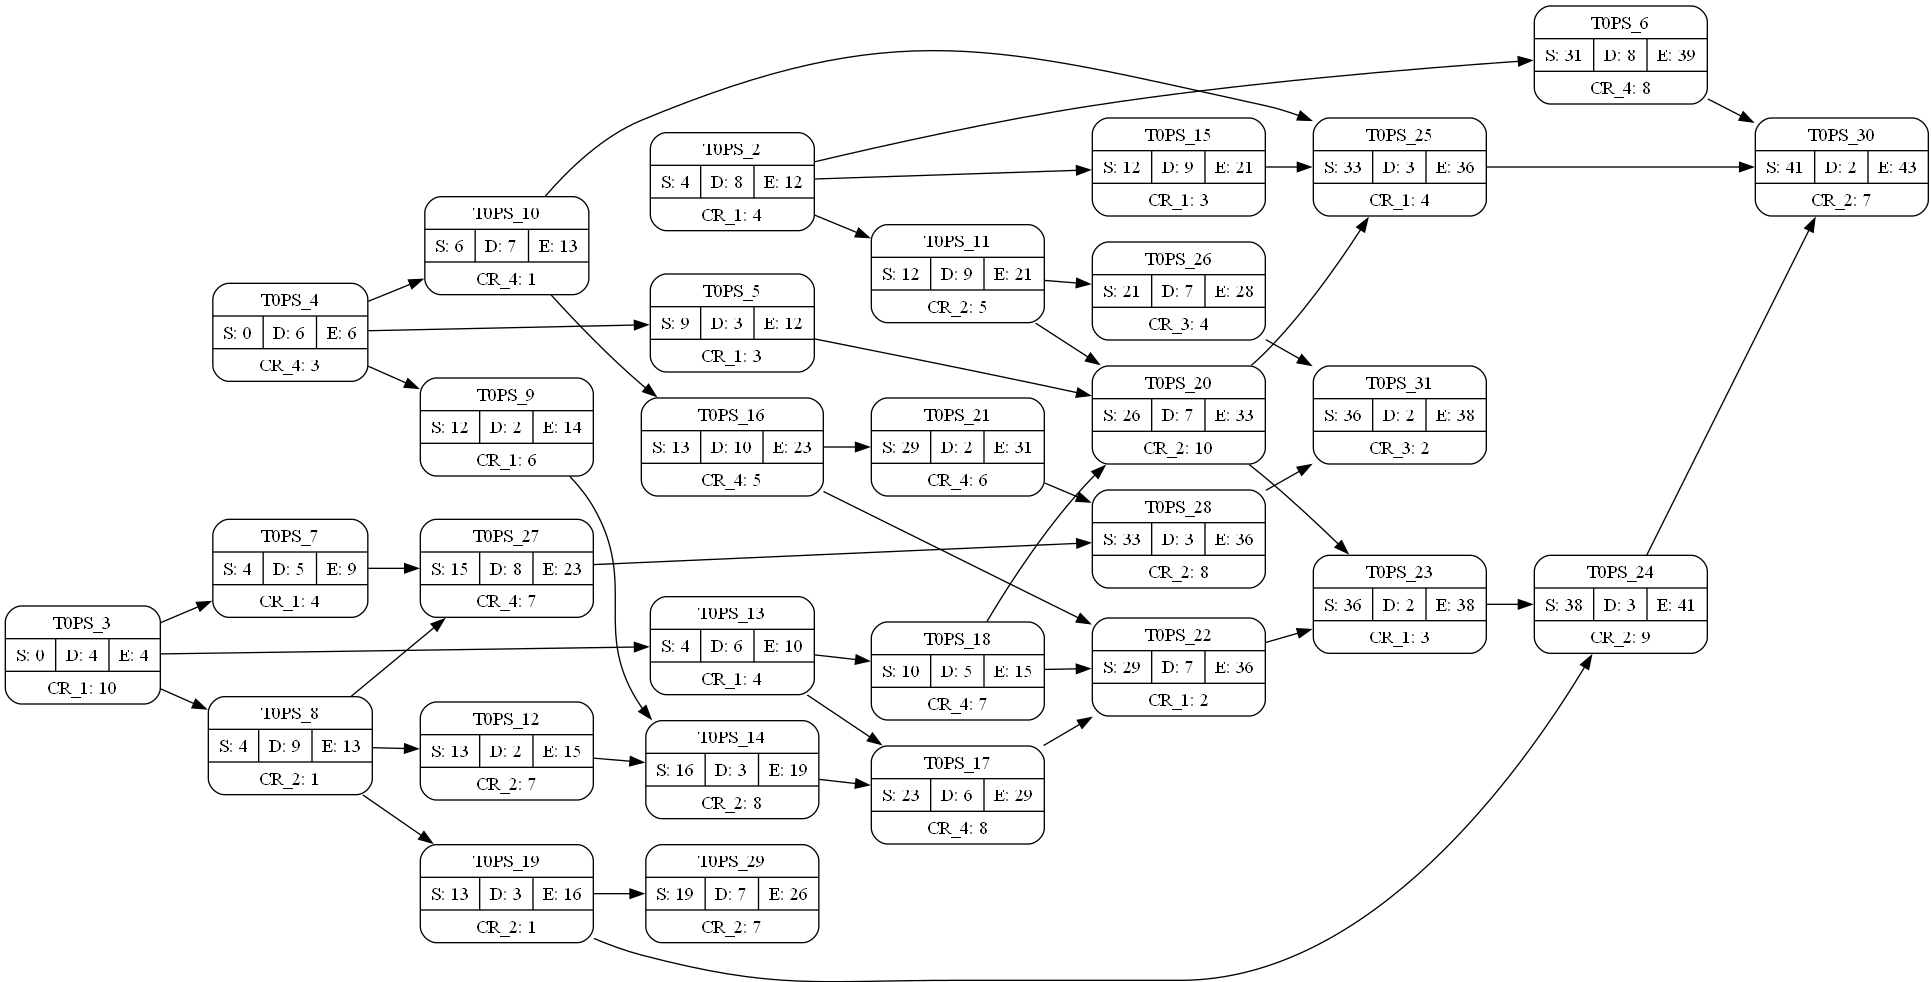
\includegraphics[width=\textwidth]{../02-concepts/images/rcpsp-pert}
% \begin{itemize}
% \item Resource constraints influence schedule, no single critical path
% \end{itemize}

% \end{frame}

% \begin{frame}
% \frametitle{RCPSP Cumulative Chart}
% 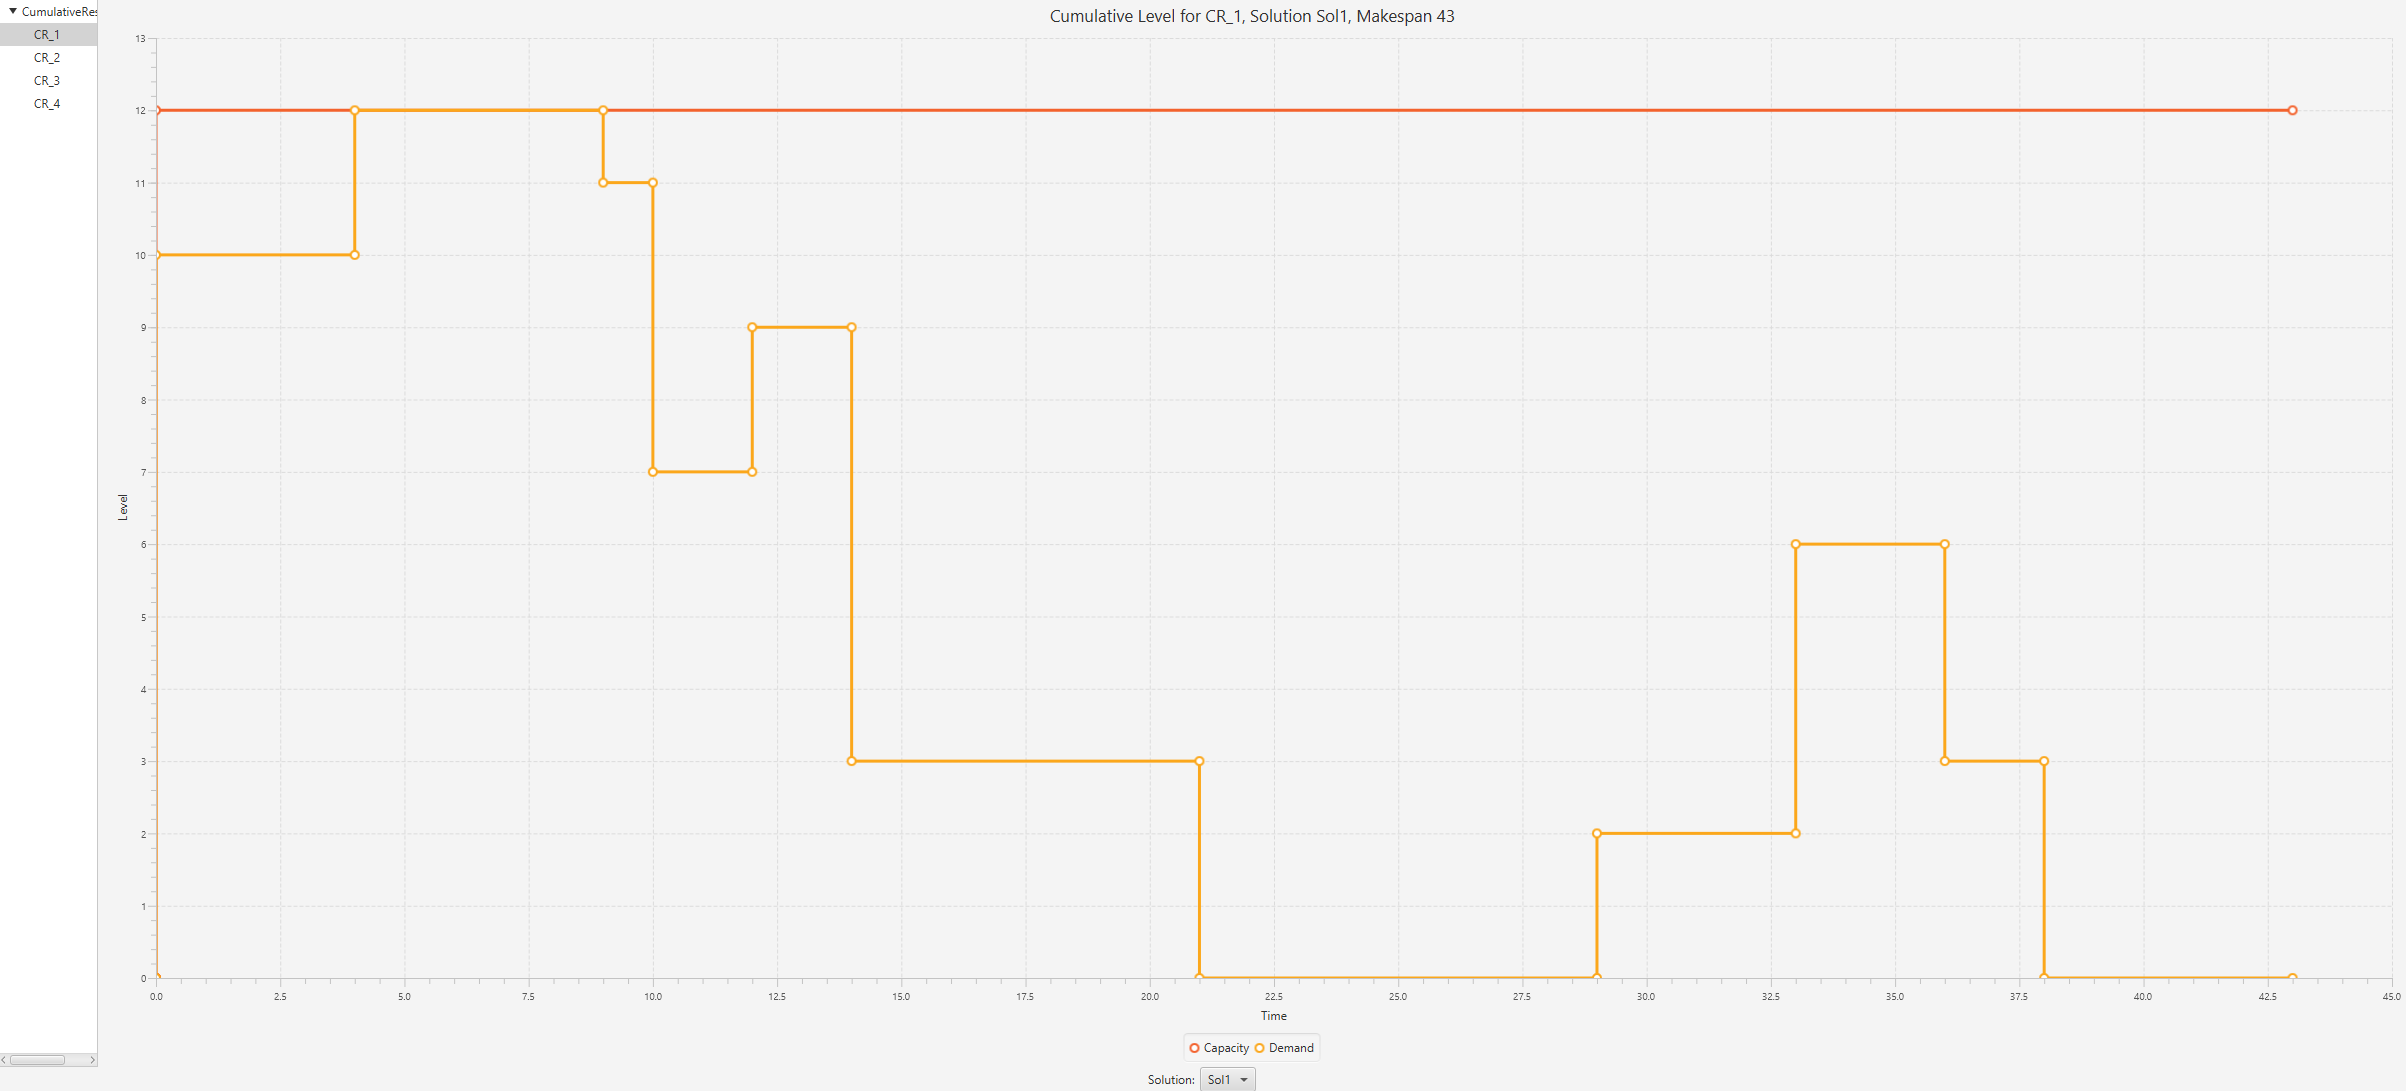
\includegraphics[width=\textwidth]{../02-concepts/images/rcpsp-cumulative-chart}
% \begin{itemize}
% \item Multiple cumulative resource, not busy all the time
% \item Not all instances are very hard to solve
% \end{itemize}

% \end{frame}

\begin{frame}
\frametitle{More on Visualization}
\begin{itemize}
\item Tutorial at CP 2021 (\url{https://cp2021.a4cp.org/tutorials.html})
\item By Helmut Simonis, Insight/UCC and Guido Tack, Monash University
\item Video at \url{https://www.youtube.com/watch?v=AI-ZfQtMLAU}
\end{itemize}
\end{frame}


\begin{frame}
\frametitle{Take-Away Message}
\begin{itemize}
\item Visualization can help at different stages of \\the development process
\item Discover problems early
\item Understand what is happening without drowning in details
\item Easily communicate with stakeholders without CP experience 
\item Decide how much integration with solver you need
\item Complex use cases require visualization to be practical
\item Generic vs. application specific visualization 
\end{itemize}
\end{frame}



\section{Literature Survey}

\begin{frame}
\frametitle{Constraint Programming and Scheduling - A Survey}
\begin{itemize}
\item Joint work with Cemalettin Ozturk, MTU
\item What is out there
\item Where to start
\item Where to publish
\item I'm interested in some specific topic, what is relevant
\item Results available at \url{https://hsimonis.github.io/pthg24/}
\end{itemize}
\end{frame}

\begin{frame}
\frametitle{Overall Analysis (Based on 1278 Works)}
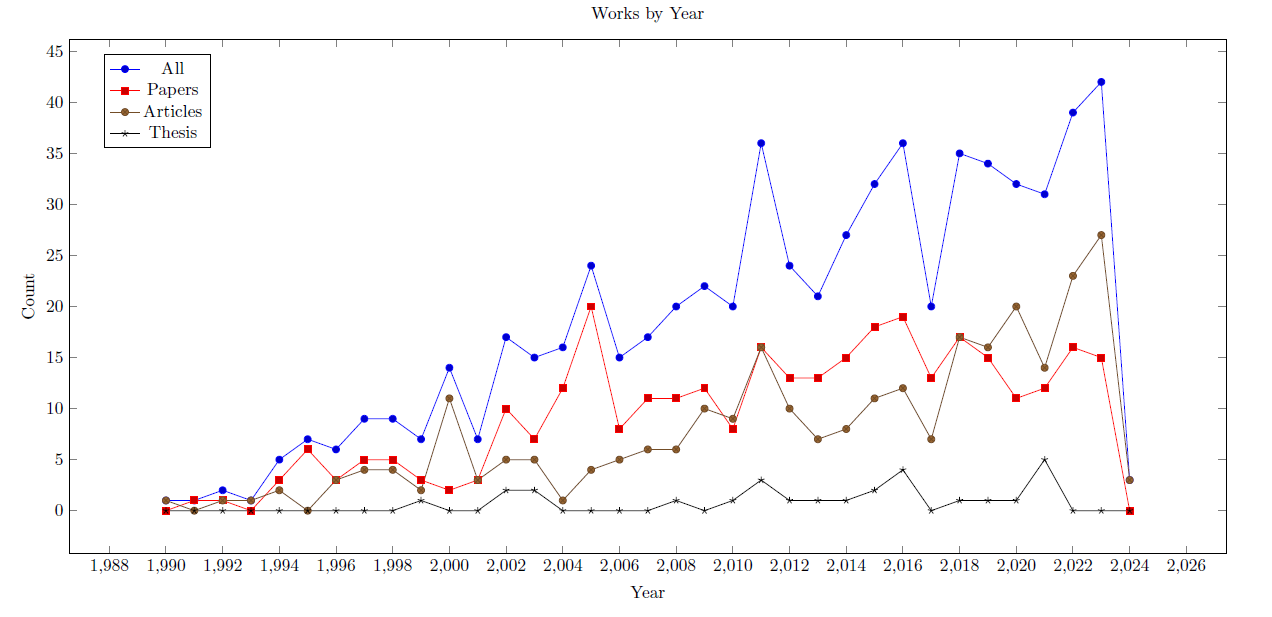
\includegraphics[width=\textwidth]{../literaturesurvey/images/worksbyyear}
\end{frame}

\begin{frame}
\frametitle{Origin of Papers}
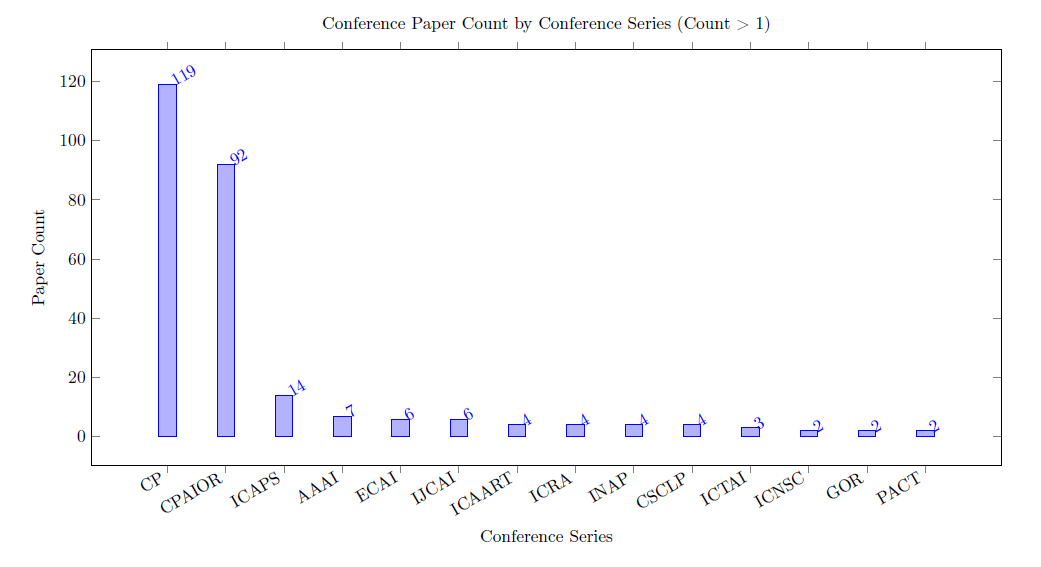
\includegraphics[width=\textwidth]{../literaturesurvey/images/conferences}
\end{frame}


\begin{frame}
\frametitle{Origin of Articles}
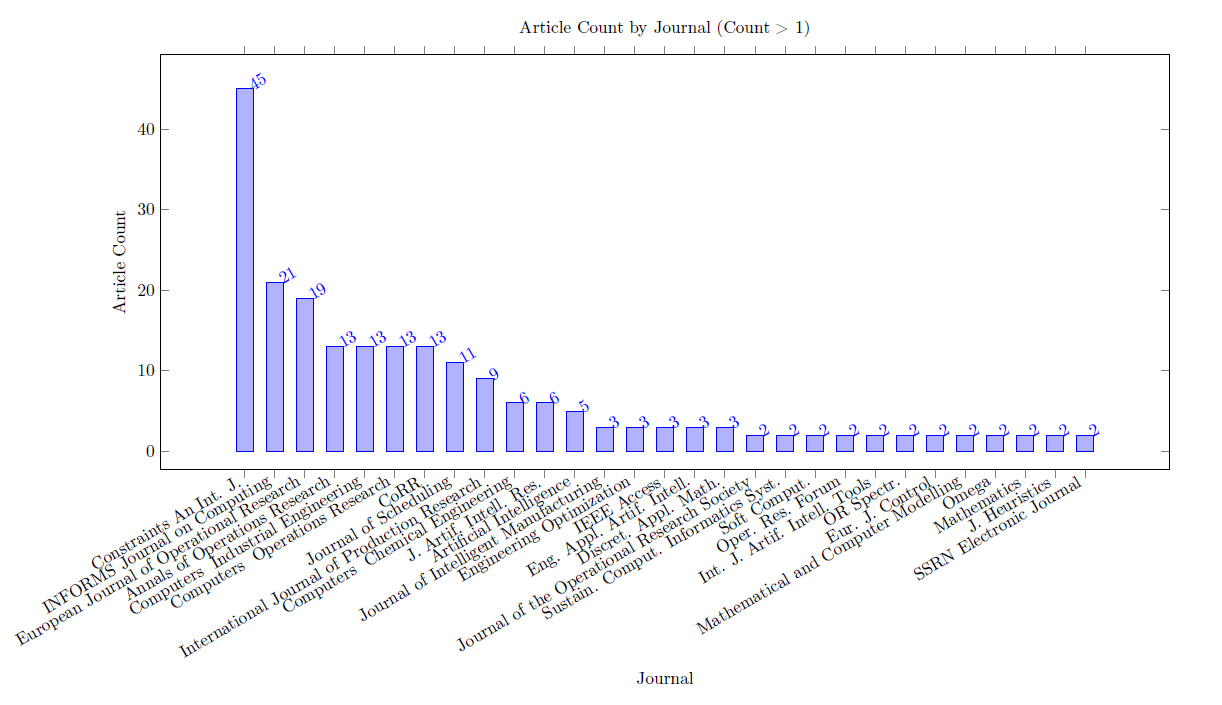
\includegraphics[width=\textwidth]{../literaturesurvey/images/journals}
\end{frame}


\begin{frame}
\frametitle{Automatically Extracted Article Features}
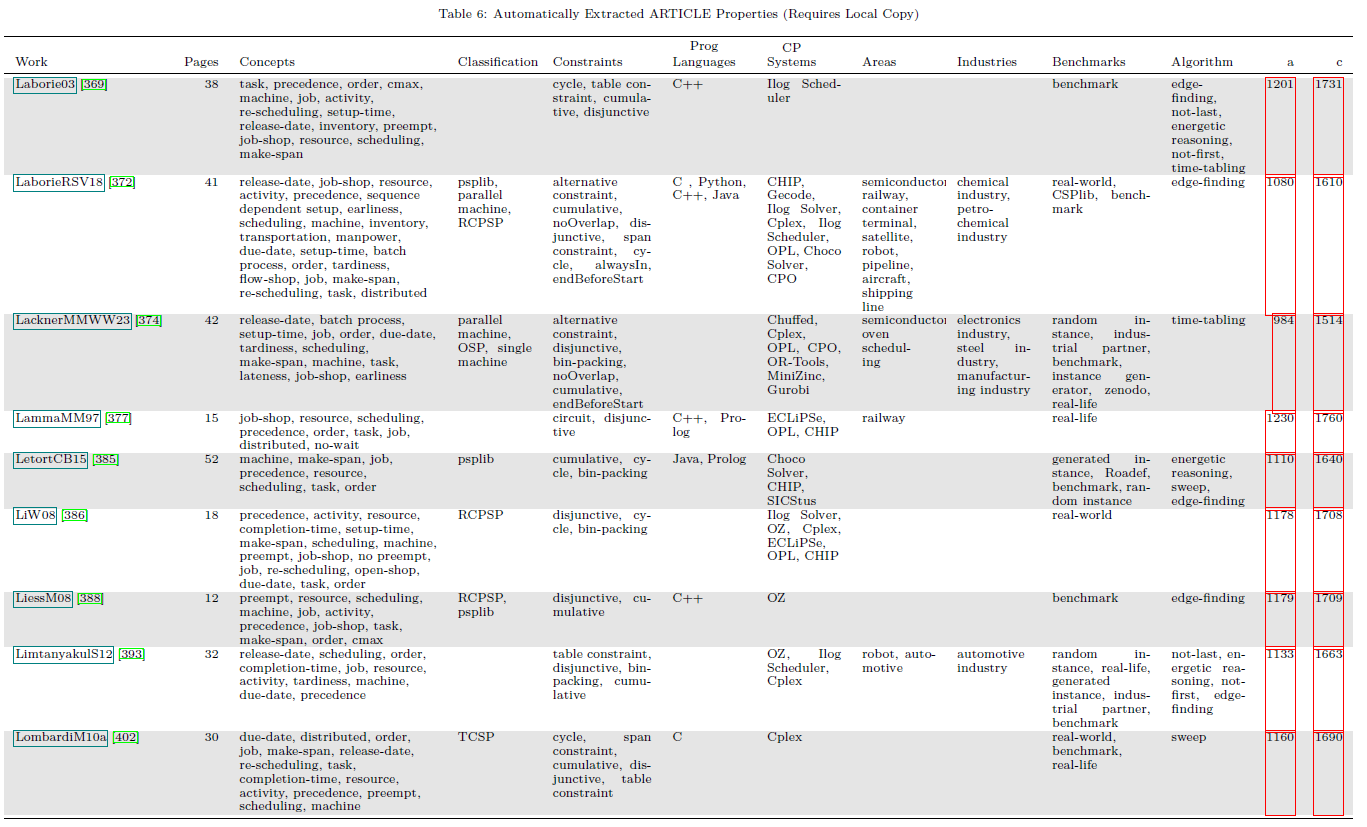
\includegraphics[width=\textwidth]{../literaturesurvey/images/extracted}
\end{frame}

\begin{frame}
\frametitle{Extracted Features: Application Areas}

\includegraphics[width=\textwidth]{../literaturesurvey/images/applicationareas}
\end{frame}

\begin{frame}
\frametitle{Co-Author Graph}
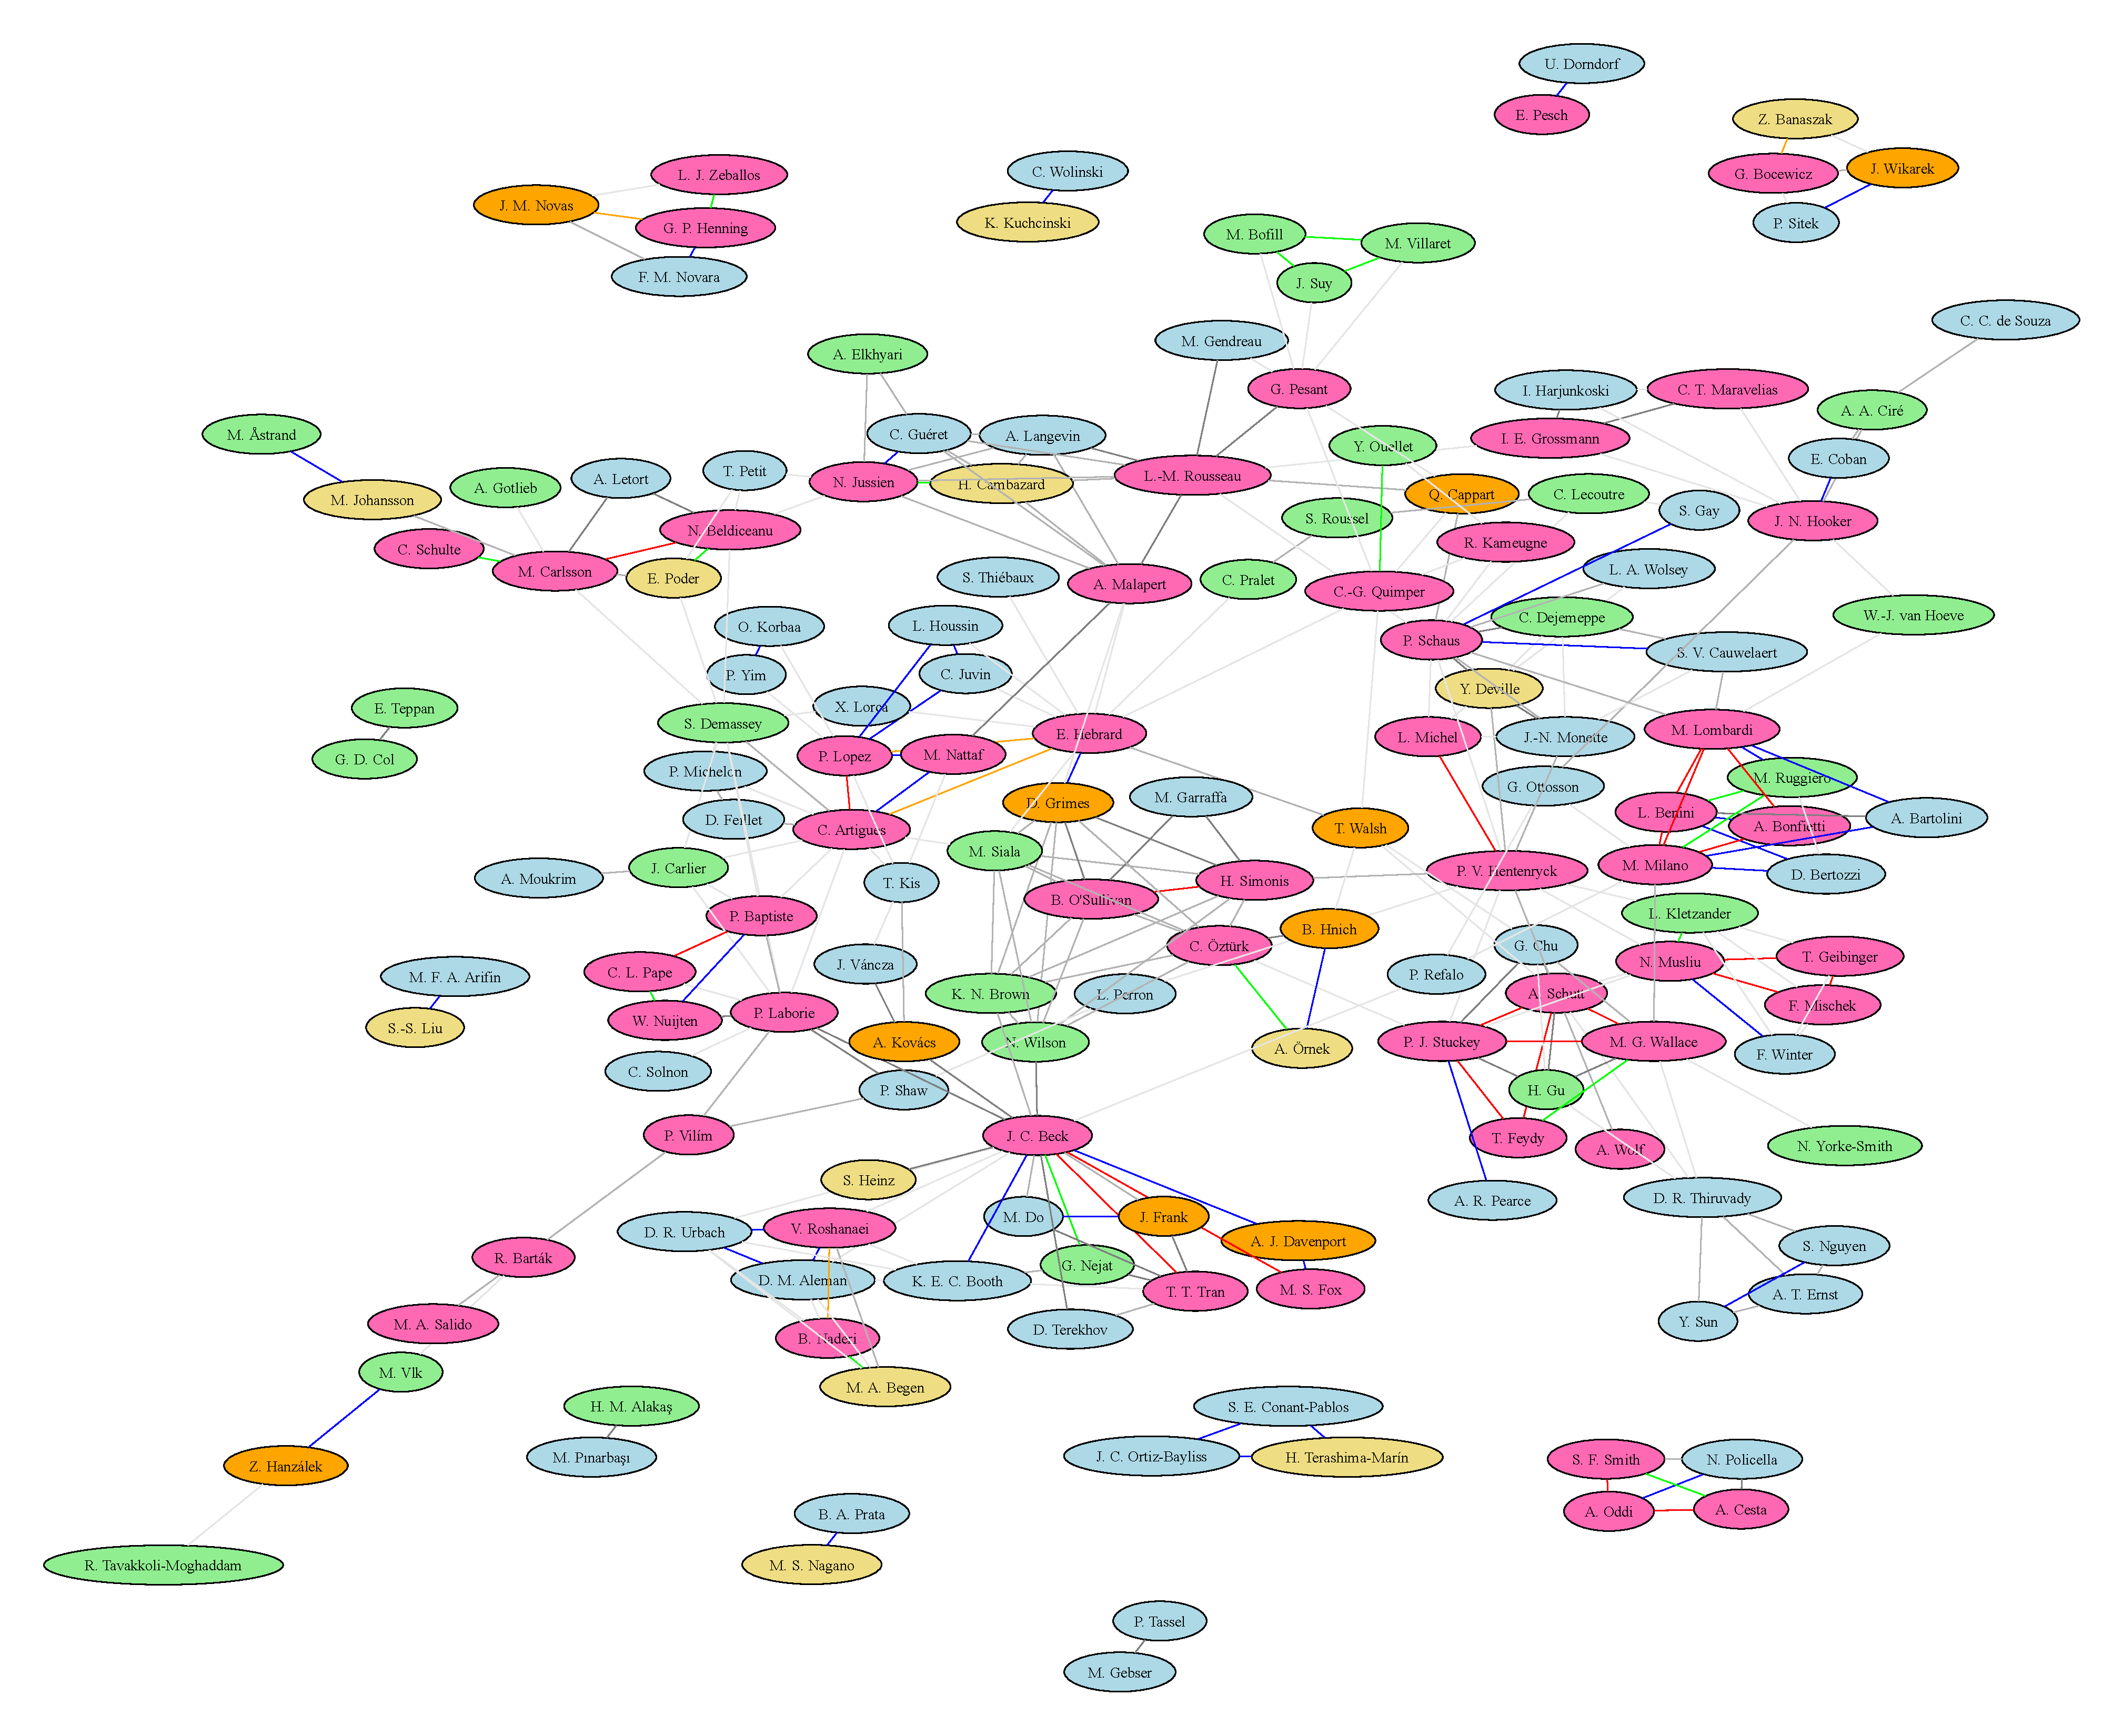
\includegraphics[width=.9\textwidth]{../schedulingseminar/images/fdp.pdf}
\end{frame}


\section{Conclusion}

\begin{frame}
\frametitle{Conclusions}
\begin{itemize}
\item Constraint Programming is a useful tool for scheduling
\item Choice of back-end solver not trivial
\begin{itemize}
\item Feature set
\item Solution quality
\item Deployment options
\item Integration with overall solution
\end{itemize}
\item Use of CP does not require deep understanding of technology
\item Visualization key to interpreting results
\item Increasing number of "CP inside" papers
\end{itemize}
\end{frame}


